\documentclass[twoside]{book}

% Packages required by doxygen
\usepackage{fixltx2e}
\usepackage{calc}
\usepackage{doxygen}
\usepackage[export]{adjustbox} % also loads graphicx
\usepackage{graphicx}
\usepackage[utf8]{inputenc}
\usepackage{makeidx}
\usepackage{multicol}
\usepackage{multirow}
\PassOptionsToPackage{warn}{textcomp}
\usepackage{textcomp}
\usepackage[nointegrals]{wasysym}
\usepackage[table]{xcolor}

% Font selection
\usepackage[T1]{fontenc}
\usepackage[scaled=.90]{helvet}
\usepackage{courier}
\usepackage{amssymb}
\usepackage{sectsty}
\renewcommand{\familydefault}{\sfdefault}
\allsectionsfont{%
  \fontseries{bc}\selectfont%
  \color{darkgray}%
}
\renewcommand{\DoxyLabelFont}{%
  \fontseries{bc}\selectfont%
  \color{darkgray}%
}
\newcommand{\+}{\discretionary{\mbox{\scriptsize$\hookleftarrow$}}{}{}}

% Page & text layout
\usepackage{geometry}
\geometry{%
  a4paper,%
  top=2.5cm,%
  bottom=2.5cm,%
  left=2.5cm,%
  right=2.5cm%
}
\tolerance=750
\hfuzz=15pt
\hbadness=750
\setlength{\emergencystretch}{15pt}
\setlength{\parindent}{0cm}
\setlength{\parskip}{0.2cm}
\makeatletter
\renewcommand{\paragraph}{%
  \@startsection{paragraph}{4}{0ex}{-1.0ex}{1.0ex}{%
    \normalfont\normalsize\bfseries\SS@parafont%
  }%
}
\renewcommand{\subparagraph}{%
  \@startsection{subparagraph}{5}{0ex}{-1.0ex}{1.0ex}{%
    \normalfont\normalsize\bfseries\SS@subparafont%
  }%
}
\makeatother

% Headers & footers
\usepackage{fancyhdr}
\pagestyle{fancyplain}
\fancyhead[LE]{\fancyplain{}{\bfseries\thepage}}
\fancyhead[CE]{\fancyplain{}{}}
\fancyhead[RE]{\fancyplain{}{\bfseries\leftmark}}
\fancyhead[LO]{\fancyplain{}{\bfseries\rightmark}}
\fancyhead[CO]{\fancyplain{}{}}
\fancyhead[RO]{\fancyplain{}{\bfseries\thepage}}
\fancyfoot[LE]{\fancyplain{}{}}
\fancyfoot[CE]{\fancyplain{}{}}
\fancyfoot[RE]{\fancyplain{}{\bfseries\scriptsize Generated on Mon Apr 11 2016 21\+:25\+:01 for Uran by Doxygen }}
\fancyfoot[LO]{\fancyplain{}{\bfseries\scriptsize Generated on Mon Apr 11 2016 21\+:25\+:01 for Uran by Doxygen }}
\fancyfoot[CO]{\fancyplain{}{}}
\fancyfoot[RO]{\fancyplain{}{}}
\renewcommand{\footrulewidth}{0.4pt}
\renewcommand{\chaptermark}[1]{%
  \markboth{#1}{}%
}
\renewcommand{\sectionmark}[1]{%
  \markright{\thesection\ #1}%
}

% Indices & bibliography
\usepackage{natbib}
\usepackage[titles]{tocloft}
\setcounter{tocdepth}{3}
\setcounter{secnumdepth}{5}
\makeindex

% Hyperlinks (required, but should be loaded last)
\usepackage{ifpdf}
\ifpdf
  \usepackage[pdftex,pagebackref=true]{hyperref}
\else
  \usepackage[ps2pdf,pagebackref=true]{hyperref}
\fi
\hypersetup{%
  colorlinks=true,%
  linkcolor=blue,%
  citecolor=blue,%
  unicode%
}

% Custom commands
\newcommand{\clearemptydoublepage}{%
  \newpage{\pagestyle{empty}\cleardoublepage}%
}


%===== C O N T E N T S =====

\begin{document}

% Titlepage & ToC
\hypersetup{pageanchor=false,
             bookmarks=true,
             bookmarksnumbered=true,
             pdfencoding=unicode
            }
\pagenumbering{roman}
\begin{titlepage}
\vspace*{7cm}
\begin{center}%
{\Large Uran }\\
\vspace*{1cm}
{\large Generated by Doxygen 1.8.9.1}\\
\vspace*{0.5cm}
{\small Mon Apr 11 2016 21:25:01}\\
\end{center}
\end{titlepage}
\clearemptydoublepage
\tableofcontents
\clearemptydoublepage
\pagenumbering{arabic}
\hypersetup{pageanchor=true}

%--- Begin generated contents ---
\chapter{Namespace Index}
\section{Namespace List}
Here is a list of all namespaces with brief descriptions\+:\begin{DoxyCompactList}
\item\contentsline{section}{\hyperlink{namespacetest}{test} }{\pageref{namespacetest}}{}
\item\contentsline{section}{\hyperlink{namespacetest_1_1formula}{test.\+formula} }{\pageref{namespacetest_1_1formula}}{}
\item\contentsline{section}{\hyperlink{namespacetest_1_1smt}{test.\+smt} }{\pageref{namespacetest_1_1smt}}{}
\item\contentsline{section}{\hyperlink{namespaceuran}{uran} }{\pageref{namespaceuran}}{}
\item\contentsline{section}{\hyperlink{namespaceuran_1_1err}{uran.\+err} }{\pageref{namespaceuran_1_1err}}{}
\item\contentsline{section}{\hyperlink{namespaceuran_1_1formula}{uran.\+formula} }{\pageref{namespaceuran_1_1formula}}{}
\item\contentsline{section}{\hyperlink{namespaceuran_1_1formula_1_1cnf}{uran.\+formula.\+cnf} }{\pageref{namespaceuran_1_1formula_1_1cnf}}{}
\item\contentsline{section}{\hyperlink{namespaceuran_1_1formula_1_1cnf_1_1visitor}{uran.\+formula.\+cnf.\+visitor} }{\pageref{namespaceuran_1_1formula_1_1cnf_1_1visitor}}{}
\item\contentsline{section}{\hyperlink{namespaceuran_1_1formula_1_1smt2}{uran.\+formula.\+smt2} }{\pageref{namespaceuran_1_1formula_1_1smt2}}{}
\item\contentsline{section}{\hyperlink{namespaceuran_1_1formula_1_1type}{uran.\+formula.\+type} }{\pageref{namespaceuran_1_1formula_1_1type}}{}
\item\contentsline{section}{\hyperlink{namespaceuran_1_1formula_1_1value}{uran.\+formula.\+value} }{\pageref{namespaceuran_1_1formula_1_1value}}{}
\item\contentsline{section}{\hyperlink{namespaceuran_1_1formula_1_1visitor}{uran.\+formula.\+visitor} }{\pageref{namespaceuran_1_1formula_1_1visitor}}{}
\item\contentsline{section}{\hyperlink{namespaceuran_1_1solver}{uran.\+solver} }{\pageref{namespaceuran_1_1solver}}{}
\item\contentsline{section}{\hyperlink{namespaceuran_1_1test}{uran.\+test} }{\pageref{namespaceuran_1_1test}}{}
\item\contentsline{section}{\hyperlink{namespaceuran_1_1test_1_1util}{uran.\+test.\+util} }{\pageref{namespaceuran_1_1test_1_1util}}{}
\end{DoxyCompactList}

\chapter{Hierarchical Index}
\section{Class Hierarchy}
This inheritance list is sorted roughly, but not completely, alphabetically\+:\begin{DoxyCompactList}
\item \contentsline{section}{uran.\+formula.\+Abstract\+Formula}{\pageref{classuran_1_1formula_1_1_abstract_formula}}{}
\begin{DoxyCompactList}
\item \contentsline{section}{uran.\+formula.\+Atomic\+Formula}{\pageref{classuran_1_1formula_1_1_atomic_formula}}{}
\item \contentsline{section}{uran.\+formula.\+Binary\+Formula}{\pageref{classuran_1_1formula_1_1_binary_formula}}{}
\begin{DoxyCompactList}
\item \contentsline{section}{uran.\+formula.\+And\+Formula}{\pageref{classuran_1_1formula_1_1_and_formula}}{}
\item \contentsline{section}{uran.\+formula.\+Arithmetic\+Formula}{\pageref{classuran_1_1formula_1_1_arithmetic_formula}}{}
\item \contentsline{section}{uran.\+formula.\+Comparison\+Formula}{\pageref{classuran_1_1formula_1_1_comparison_formula}}{}
\item \contentsline{section}{uran.\+formula.\+Eq\+Formula}{\pageref{classuran_1_1formula_1_1_eq_formula}}{}
\item \contentsline{section}{uran.\+formula.\+Implies\+Formula}{\pageref{classuran_1_1formula_1_1_implies_formula}}{}
\item \contentsline{section}{uran.\+formula.\+One\+Formula}{\pageref{classuran_1_1formula_1_1_one_formula}}{}
\item \contentsline{section}{uran.\+formula.\+Or\+Formula}{\pageref{classuran_1_1formula_1_1_or_formula}}{}
\end{DoxyCompactList}
\item \contentsline{section}{uran.\+formula.\+Decls}{\pageref{classuran_1_1formula_1_1_decls}}{}
\item \contentsline{section}{uran.\+formula.\+Function}{\pageref{classuran_1_1formula_1_1_function}}{}
\begin{DoxyCompactList}
\item \contentsline{section}{uran.\+formula.\+Constant}{\pageref{classuran_1_1formula_1_1_constant}}{}
\begin{DoxyCompactList}
\item \contentsline{section}{uran.\+formula.\+Variable}{\pageref{classuran_1_1formula_1_1_variable}}{}
\end{DoxyCompactList}
\end{DoxyCompactList}
\item \contentsline{section}{uran.\+formula.\+Literal}{\pageref{classuran_1_1formula_1_1_literal}}{}
\begin{DoxyCompactList}
\item \contentsline{section}{uran.\+formula.\+Bool\+Literal}{\pageref{classuran_1_1formula_1_1_bool_literal}}{}
\item \contentsline{section}{uran.\+formula.\+Num\+Literal}{\pageref{classuran_1_1formula_1_1_num_literal}}{}
\end{DoxyCompactList}
\item \contentsline{section}{uran.\+formula.\+Quantified\+Formula}{\pageref{classuran_1_1formula_1_1_quantified_formula}}{}
\item \contentsline{section}{uran.\+formula.\+Scope}{\pageref{classuran_1_1formula_1_1_scope}}{}
\item \contentsline{section}{uran.\+formula.\+Ternary\+Formula}{\pageref{classuran_1_1formula_1_1_ternary_formula}}{}
\item \contentsline{section}{uran.\+formula.\+Unary\+Formula}{\pageref{classuran_1_1formula_1_1_unary_formula}}{}
\begin{DoxyCompactList}
\item \contentsline{section}{uran.\+formula.\+Neg\+Formula}{\pageref{classuran_1_1formula_1_1_neg_formula}}{}
\end{DoxyCompactList}
\end{DoxyCompactList}
\item \contentsline{section}{uran.\+formula.\+cnf.\+visitor.\+Abstract\+Visitor}{\pageref{classuran_1_1formula_1_1cnf_1_1visitor_1_1_abstract_visitor}}{}
\begin{DoxyCompactList}
\item \contentsline{section}{uran.\+formula.\+cnf.\+C\+N\+F\+Translator}{\pageref{classuran_1_1formula_1_1cnf_1_1_c_n_f_translator}}{}
\end{DoxyCompactList}
\item \contentsline{section}{uran.\+formula.\+visitor.\+Abstract\+Visitor}{\pageref{classuran_1_1formula_1_1visitor_1_1_abstract_visitor}}{}
\begin{DoxyCompactList}
\item \contentsline{section}{uran.\+formula.\+smt2.\+S\+M\+T2\+Writer}{\pageref{classuran_1_1formula_1_1smt2_1_1_s_m_t2_writer}}{}
\end{DoxyCompactList}
\item \contentsline{section}{uran.\+test.\+util.\+Color}{\pageref{classuran_1_1test_1_1util_1_1_color}}{}
\item \contentsline{section}{test.\+formula.\+Color}{\pageref{classtest_1_1formula_1_1_color}}{}
\item \contentsline{section}{uran.\+test.\+util.\+Color\+Print}{\pageref{classuran_1_1test_1_1util_1_1_color_print}}{}
\item \contentsline{section}{test.\+formula.\+Color\+Print}{\pageref{classtest_1_1formula_1_1_color_print}}{}
\item \contentsline{section}{uran.\+formula.\+Connective}{\pageref{enumuran_1_1formula_1_1_connective}}{}
\item \contentsline{section}{uran.\+formula.\+Formula\+Builder}{\pageref{classuran_1_1formula_1_1_formula_builder}}{}
\item \contentsline{section}{uran.\+formula.\+Function\+Factory}{\pageref{classuran_1_1formula_1_1_function_factory}}{}
\item \contentsline{section}{uran.\+formula.\+cnf.\+Node}{\pageref{classuran_1_1formula_1_1cnf_1_1_node}}{}
\begin{DoxyCompactList}
\item \contentsline{section}{uran.\+formula.\+cnf.\+Boolean\+Circuit}{\pageref{classuran_1_1formula_1_1cnf_1_1_boolean_circuit}}{}
\begin{DoxyCompactList}
\item \contentsline{section}{uran.\+formula.\+cnf.\+Binary\+Gate}{\pageref{classuran_1_1formula_1_1cnf_1_1_binary_gate}}{}
\item \contentsline{section}{uran.\+formula.\+cnf.\+Boolean\+Variable}{\pageref{classuran_1_1formula_1_1cnf_1_1_boolean_variable}}{}
\item \contentsline{section}{uran.\+formula.\+cnf.\+Not\+Gate}{\pageref{classuran_1_1formula_1_1cnf_1_1_not_gate}}{}
\end{DoxyCompactList}
\item \contentsline{section}{uran.\+formula.\+cnf.\+Operator}{\pageref{classuran_1_1formula_1_1cnf_1_1_operator}}{}
\end{DoxyCompactList}
\item \contentsline{section}{uran.\+formula.\+Quantifier}{\pageref{enumuran_1_1formula_1_1_quantifier}}{}
\item \contentsline{section}{uran.\+solver.\+Result}{\pageref{enumuran_1_1solver_1_1_result}}{}
\item Runnable\begin{DoxyCompactList}
\item \contentsline{section}{uran.\+formula.\+smt2.\+S\+M\+T2\+Writer}{\pageref{classuran_1_1formula_1_1smt2_1_1_s_m_t2_writer}}{}
\end{DoxyCompactList}
\item Runtime\+Exception\begin{DoxyCompactList}
\item \contentsline{section}{uran.\+err.\+Abstract\+Exception}{\pageref{classuran_1_1err_1_1_abstract_exception}}{}
\begin{DoxyCompactList}
\item \contentsline{section}{uran.\+err.\+Argument\+Size\+Exception}{\pageref{classuran_1_1err_1_1_argument_size_exception}}{}
\item \contentsline{section}{uran.\+err.\+Duplicated\+Declaration}{\pageref{classuran_1_1err_1_1_duplicated_declaration}}{}
\item \contentsline{section}{uran.\+err.\+Ill\+Formed\+Formula\+Exception}{\pageref{classuran_1_1err_1_1_ill_formed_formula_exception}}{}
\item \contentsline{section}{uran.\+err.\+Miss\+File\+Name\+Exception}{\pageref{classuran_1_1err_1_1_miss_file_name_exception}}{}
\item \contentsline{section}{uran.\+err.\+Missing\+Formula\+Exception}{\pageref{classuran_1_1err_1_1_missing_formula_exception}}{}
\item \contentsline{section}{uran.\+err.\+Nullable\+Formula\+Exception}{\pageref{classuran_1_1err_1_1_nullable_formula_exception}}{}
\item \contentsline{section}{uran.\+err.\+Type\+Missmatch\+Exception}{\pageref{classuran_1_1err_1_1_type_missmatch_exception}}{}
\item \contentsline{section}{uran.\+err.\+Unknown\+Exception}{\pageref{classuran_1_1err_1_1_unknown_exception}}{}
\item \contentsline{section}{uran.\+err.\+Unsat\+Exception}{\pageref{classuran_1_1err_1_1_unsat_exception}}{}
\item \contentsline{section}{uran.\+err.\+Var\+Exists\+Exception}{\pageref{classuran_1_1err_1_1_var_exists_exception}}{}
\item \contentsline{section}{uran.\+err.\+Var\+Null\+Exception}{\pageref{classuran_1_1err_1_1_var_null_exception}}{}
\end{DoxyCompactList}
\end{DoxyCompactList}
\item \contentsline{section}{test.\+formula.\+test\+Boolean\+Circuit}{\pageref{classtest_1_1formula_1_1test_boolean_circuit}}{}
\item \contentsline{section}{test.\+formula.\+test\+Formula}{\pageref{classtest_1_1formula_1_1test_formula}}{}
\item \contentsline{section}{test.\+smt.\+test\+S\+M\+T\+Solving}{\pageref{classtest_1_1smt_1_1test_s_m_t_solving}}{}
\item \contentsline{section}{uran.\+formula.\+cnf.\+Translator}{\pageref{interfaceuran_1_1formula_1_1cnf_1_1_translator}}{}
\begin{DoxyCompactList}
\item \contentsline{section}{uran.\+formula.\+cnf.\+C\+N\+F\+Translator}{\pageref{classuran_1_1formula_1_1cnf_1_1_c_n_f_translator}}{}
\end{DoxyCompactList}
\item \contentsline{section}{uran.\+formula.\+type.\+Type}{\pageref{classuran_1_1formula_1_1type_1_1_type}}{}
\begin{DoxyCompactList}
\item \contentsline{section}{uran.\+formula.\+type.\+Bool}{\pageref{classuran_1_1formula_1_1type_1_1_bool}}{}
\item \contentsline{section}{uran.\+formula.\+type.\+Int}{\pageref{classuran_1_1formula_1_1type_1_1_int}}{}
\item \contentsline{section}{uran.\+formula.\+type.\+Real}{\pageref{classuran_1_1formula_1_1type_1_1_real}}{}
\item \contentsline{section}{uran.\+formula.\+type.\+Sort}{\pageref{classuran_1_1formula_1_1type_1_1_sort}}{}
\end{DoxyCompactList}
\item \contentsline{section}{uran.\+formula.\+value.\+Value}{\pageref{classuran_1_1formula_1_1value_1_1_value}}{}
\begin{DoxyCompactList}
\item \contentsline{section}{uran.\+formula.\+value.\+Bool\+Value}{\pageref{classuran_1_1formula_1_1value_1_1_bool_value}}{}
\item \contentsline{section}{uran.\+formula.\+value.\+Int\+Value}{\pageref{classuran_1_1formula_1_1value_1_1_int_value}}{}
\end{DoxyCompactList}
\item \contentsline{section}{uran.\+solver.\+Z3\+S\+M\+T2\+Solver}{\pageref{classuran_1_1solver_1_1_z3_s_m_t2_solver}}{}
\end{DoxyCompactList}

\chapter{Class Index}
\section{Class List}
Here are the classes, structs, unions and interfaces with brief descriptions\+:\begin{DoxyCompactList}
\item\contentsline{section}{\hyperlink{classuran_1_1err_1_1_abstract_exception}{uran.\+err.\+Abstract\+Exception} }{\pageref{classuran_1_1err_1_1_abstract_exception}}{}
\item\contentsline{section}{\hyperlink{classuran_1_1formula_1_1_abstract_formula}{uran.\+formula.\+Abstract\+Formula} }{\pageref{classuran_1_1formula_1_1_abstract_formula}}{}
\item\contentsline{section}{\hyperlink{classuran_1_1formula_1_1cnf_1_1visitor_1_1_abstract_visitor}{uran.\+formula.\+cnf.\+visitor.\+Abstract\+Visitor} }{\pageref{classuran_1_1formula_1_1cnf_1_1visitor_1_1_abstract_visitor}}{}
\item\contentsline{section}{\hyperlink{classuran_1_1formula_1_1visitor_1_1_abstract_visitor}{uran.\+formula.\+visitor.\+Abstract\+Visitor} }{\pageref{classuran_1_1formula_1_1visitor_1_1_abstract_visitor}}{}
\item\contentsline{section}{\hyperlink{classuran_1_1formula_1_1_and_formula}{uran.\+formula.\+And\+Formula} }{\pageref{classuran_1_1formula_1_1_and_formula}}{}
\item\contentsline{section}{\hyperlink{classuran_1_1err_1_1_argument_size_exception}{uran.\+err.\+Argument\+Size\+Exception} }{\pageref{classuran_1_1err_1_1_argument_size_exception}}{}
\item\contentsline{section}{\hyperlink{classuran_1_1formula_1_1_arithmetic_formula}{uran.\+formula.\+Arithmetic\+Formula} }{\pageref{classuran_1_1formula_1_1_arithmetic_formula}}{}
\item\contentsline{section}{\hyperlink{classuran_1_1formula_1_1_atomic_formula}{uran.\+formula.\+Atomic\+Formula} }{\pageref{classuran_1_1formula_1_1_atomic_formula}}{}
\item\contentsline{section}{\hyperlink{classuran_1_1formula_1_1_binary_formula}{uran.\+formula.\+Binary\+Formula} }{\pageref{classuran_1_1formula_1_1_binary_formula}}{}
\item\contentsline{section}{\hyperlink{classuran_1_1formula_1_1cnf_1_1_binary_gate}{uran.\+formula.\+cnf.\+Binary\+Gate} }{\pageref{classuran_1_1formula_1_1cnf_1_1_binary_gate}}{}
\item\contentsline{section}{\hyperlink{classuran_1_1formula_1_1type_1_1_bool}{uran.\+formula.\+type.\+Bool} }{\pageref{classuran_1_1formula_1_1type_1_1_bool}}{}
\item\contentsline{section}{\hyperlink{classuran_1_1formula_1_1cnf_1_1_boolean_circuit}{uran.\+formula.\+cnf.\+Boolean\+Circuit} }{\pageref{classuran_1_1formula_1_1cnf_1_1_boolean_circuit}}{}
\item\contentsline{section}{\hyperlink{classuran_1_1formula_1_1cnf_1_1_boolean_variable}{uran.\+formula.\+cnf.\+Boolean\+Variable} }{\pageref{classuran_1_1formula_1_1cnf_1_1_boolean_variable}}{}
\item\contentsline{section}{\hyperlink{classuran_1_1formula_1_1_bool_literal}{uran.\+formula.\+Bool\+Literal} }{\pageref{classuran_1_1formula_1_1_bool_literal}}{}
\item\contentsline{section}{\hyperlink{classuran_1_1formula_1_1value_1_1_bool_value}{uran.\+formula.\+value.\+Bool\+Value} }{\pageref{classuran_1_1formula_1_1value_1_1_bool_value}}{}
\item\contentsline{section}{\hyperlink{classuran_1_1formula_1_1cnf_1_1_c_n_f_translator}{uran.\+formula.\+cnf.\+C\+N\+F\+Translator} }{\pageref{classuran_1_1formula_1_1cnf_1_1_c_n_f_translator}}{}
\item\contentsline{section}{\hyperlink{classuran_1_1test_1_1util_1_1_color}{uran.\+test.\+util.\+Color} }{\pageref{classuran_1_1test_1_1util_1_1_color}}{}
\item\contentsline{section}{\hyperlink{classtest_1_1formula_1_1_color}{test.\+formula.\+Color} }{\pageref{classtest_1_1formula_1_1_color}}{}
\item\contentsline{section}{\hyperlink{classuran_1_1test_1_1util_1_1_color_print}{uran.\+test.\+util.\+Color\+Print} }{\pageref{classuran_1_1test_1_1util_1_1_color_print}}{}
\item\contentsline{section}{\hyperlink{classtest_1_1formula_1_1_color_print}{test.\+formula.\+Color\+Print} }{\pageref{classtest_1_1formula_1_1_color_print}}{}
\item\contentsline{section}{\hyperlink{classuran_1_1formula_1_1_comparison_formula}{uran.\+formula.\+Comparison\+Formula} }{\pageref{classuran_1_1formula_1_1_comparison_formula}}{}
\item\contentsline{section}{\hyperlink{enumuran_1_1formula_1_1_connective}{uran.\+formula.\+Connective} }{\pageref{enumuran_1_1formula_1_1_connective}}{}
\item\contentsline{section}{\hyperlink{classuran_1_1formula_1_1_constant}{uran.\+formula.\+Constant} }{\pageref{classuran_1_1formula_1_1_constant}}{}
\item\contentsline{section}{\hyperlink{classuran_1_1formula_1_1_decls}{uran.\+formula.\+Decls} }{\pageref{classuran_1_1formula_1_1_decls}}{}
\item\contentsline{section}{\hyperlink{classuran_1_1err_1_1_duplicated_declaration}{uran.\+err.\+Duplicated\+Declaration} }{\pageref{classuran_1_1err_1_1_duplicated_declaration}}{}
\item\contentsline{section}{\hyperlink{classuran_1_1formula_1_1_eq_formula}{uran.\+formula.\+Eq\+Formula} }{\pageref{classuran_1_1formula_1_1_eq_formula}}{}
\item\contentsline{section}{\hyperlink{classuran_1_1formula_1_1_formula_builder}{uran.\+formula.\+Formula\+Builder} }{\pageref{classuran_1_1formula_1_1_formula_builder}}{}
\item\contentsline{section}{\hyperlink{classuran_1_1formula_1_1_function}{uran.\+formula.\+Function} }{\pageref{classuran_1_1formula_1_1_function}}{}
\item\contentsline{section}{\hyperlink{classuran_1_1formula_1_1_function_factory}{uran.\+formula.\+Function\+Factory} }{\pageref{classuran_1_1formula_1_1_function_factory}}{}
\item\contentsline{section}{\hyperlink{classuran_1_1err_1_1_ill_formed_formula_exception}{uran.\+err.\+Ill\+Formed\+Formula\+Exception} }{\pageref{classuran_1_1err_1_1_ill_formed_formula_exception}}{}
\item\contentsline{section}{\hyperlink{classuran_1_1formula_1_1_implies_formula}{uran.\+formula.\+Implies\+Formula} }{\pageref{classuran_1_1formula_1_1_implies_formula}}{}
\item\contentsline{section}{\hyperlink{classuran_1_1formula_1_1type_1_1_int}{uran.\+formula.\+type.\+Int} }{\pageref{classuran_1_1formula_1_1type_1_1_int}}{}
\item\contentsline{section}{\hyperlink{classuran_1_1formula_1_1value_1_1_int_value}{uran.\+formula.\+value.\+Int\+Value} }{\pageref{classuran_1_1formula_1_1value_1_1_int_value}}{}
\item\contentsline{section}{\hyperlink{classuran_1_1formula_1_1_literal}{uran.\+formula.\+Literal} }{\pageref{classuran_1_1formula_1_1_literal}}{}
\item\contentsline{section}{\hyperlink{classuran_1_1err_1_1_miss_file_name_exception}{uran.\+err.\+Miss\+File\+Name\+Exception} }{\pageref{classuran_1_1err_1_1_miss_file_name_exception}}{}
\item\contentsline{section}{\hyperlink{classuran_1_1err_1_1_missing_formula_exception}{uran.\+err.\+Missing\+Formula\+Exception} }{\pageref{classuran_1_1err_1_1_missing_formula_exception}}{}
\item\contentsline{section}{\hyperlink{classuran_1_1formula_1_1_neg_formula}{uran.\+formula.\+Neg\+Formula} }{\pageref{classuran_1_1formula_1_1_neg_formula}}{}
\item\contentsline{section}{\hyperlink{classuran_1_1formula_1_1cnf_1_1_node}{uran.\+formula.\+cnf.\+Node} }{\pageref{classuran_1_1formula_1_1cnf_1_1_node}}{}
\item\contentsline{section}{\hyperlink{classuran_1_1formula_1_1cnf_1_1_not_gate}{uran.\+formula.\+cnf.\+Not\+Gate} }{\pageref{classuran_1_1formula_1_1cnf_1_1_not_gate}}{}
\item\contentsline{section}{\hyperlink{classuran_1_1err_1_1_nullable_formula_exception}{uran.\+err.\+Nullable\+Formula\+Exception} }{\pageref{classuran_1_1err_1_1_nullable_formula_exception}}{}
\item\contentsline{section}{\hyperlink{classuran_1_1formula_1_1_num_literal}{uran.\+formula.\+Num\+Literal} }{\pageref{classuran_1_1formula_1_1_num_literal}}{}
\item\contentsline{section}{\hyperlink{classuran_1_1formula_1_1_one_formula}{uran.\+formula.\+One\+Formula} }{\pageref{classuran_1_1formula_1_1_one_formula}}{}
\item\contentsline{section}{\hyperlink{classuran_1_1formula_1_1cnf_1_1_operator}{uran.\+formula.\+cnf.\+Operator} }{\pageref{classuran_1_1formula_1_1cnf_1_1_operator}}{}
\item\contentsline{section}{\hyperlink{classuran_1_1formula_1_1_or_formula}{uran.\+formula.\+Or\+Formula} }{\pageref{classuran_1_1formula_1_1_or_formula}}{}
\item\contentsline{section}{\hyperlink{classuran_1_1formula_1_1_quantified_formula}{uran.\+formula.\+Quantified\+Formula} }{\pageref{classuran_1_1formula_1_1_quantified_formula}}{}
\item\contentsline{section}{\hyperlink{enumuran_1_1formula_1_1_quantifier}{uran.\+formula.\+Quantifier} }{\pageref{enumuran_1_1formula_1_1_quantifier}}{}
\item\contentsline{section}{\hyperlink{classuran_1_1formula_1_1type_1_1_real}{uran.\+formula.\+type.\+Real} }{\pageref{classuran_1_1formula_1_1type_1_1_real}}{}
\item\contentsline{section}{\hyperlink{enumuran_1_1solver_1_1_result}{uran.\+solver.\+Result} }{\pageref{enumuran_1_1solver_1_1_result}}{}
\item\contentsline{section}{\hyperlink{classuran_1_1formula_1_1_scope}{uran.\+formula.\+Scope} }{\pageref{classuran_1_1formula_1_1_scope}}{}
\item\contentsline{section}{\hyperlink{classuran_1_1formula_1_1smt2_1_1_s_m_t2_writer}{uran.\+formula.\+smt2.\+S\+M\+T2\+Writer} }{\pageref{classuran_1_1formula_1_1smt2_1_1_s_m_t2_writer}}{}
\item\contentsline{section}{\hyperlink{classuran_1_1formula_1_1type_1_1_sort}{uran.\+formula.\+type.\+Sort} }{\pageref{classuran_1_1formula_1_1type_1_1_sort}}{}
\item\contentsline{section}{\hyperlink{classuran_1_1formula_1_1_ternary_formula}{uran.\+formula.\+Ternary\+Formula} }{\pageref{classuran_1_1formula_1_1_ternary_formula}}{}
\item\contentsline{section}{\hyperlink{classtest_1_1formula_1_1test_boolean_circuit}{test.\+formula.\+test\+Boolean\+Circuit} }{\pageref{classtest_1_1formula_1_1test_boolean_circuit}}{}
\item\contentsline{section}{\hyperlink{classtest_1_1formula_1_1test_formula}{test.\+formula.\+test\+Formula} }{\pageref{classtest_1_1formula_1_1test_formula}}{}
\item\contentsline{section}{\hyperlink{classtest_1_1smt_1_1test_s_m_t_solving}{test.\+smt.\+test\+S\+M\+T\+Solving} }{\pageref{classtest_1_1smt_1_1test_s_m_t_solving}}{}
\item\contentsline{section}{\hyperlink{interfaceuran_1_1formula_1_1cnf_1_1_translator}{uran.\+formula.\+cnf.\+Translator} }{\pageref{interfaceuran_1_1formula_1_1cnf_1_1_translator}}{}
\item\contentsline{section}{\hyperlink{classuran_1_1formula_1_1type_1_1_type}{uran.\+formula.\+type.\+Type} }{\pageref{classuran_1_1formula_1_1type_1_1_type}}{}
\item\contentsline{section}{\hyperlink{classuran_1_1err_1_1_type_missmatch_exception}{uran.\+err.\+Type\+Missmatch\+Exception} }{\pageref{classuran_1_1err_1_1_type_missmatch_exception}}{}
\item\contentsline{section}{\hyperlink{classuran_1_1formula_1_1_unary_formula}{uran.\+formula.\+Unary\+Formula} }{\pageref{classuran_1_1formula_1_1_unary_formula}}{}
\item\contentsline{section}{\hyperlink{classuran_1_1err_1_1_unknown_exception}{uran.\+err.\+Unknown\+Exception} }{\pageref{classuran_1_1err_1_1_unknown_exception}}{}
\item\contentsline{section}{\hyperlink{classuran_1_1err_1_1_unsat_exception}{uran.\+err.\+Unsat\+Exception} }{\pageref{classuran_1_1err_1_1_unsat_exception}}{}
\item\contentsline{section}{\hyperlink{classuran_1_1formula_1_1value_1_1_value}{uran.\+formula.\+value.\+Value} }{\pageref{classuran_1_1formula_1_1value_1_1_value}}{}
\item\contentsline{section}{\hyperlink{classuran_1_1err_1_1_var_exists_exception}{uran.\+err.\+Var\+Exists\+Exception} }{\pageref{classuran_1_1err_1_1_var_exists_exception}}{}
\item\contentsline{section}{\hyperlink{classuran_1_1formula_1_1_variable}{uran.\+formula.\+Variable} }{\pageref{classuran_1_1formula_1_1_variable}}{}
\item\contentsline{section}{\hyperlink{classuran_1_1err_1_1_var_null_exception}{uran.\+err.\+Var\+Null\+Exception} }{\pageref{classuran_1_1err_1_1_var_null_exception}}{}
\item\contentsline{section}{\hyperlink{classuran_1_1solver_1_1_z3_s_m_t2_solver}{uran.\+solver.\+Z3\+S\+M\+T2\+Solver} }{\pageref{classuran_1_1solver_1_1_z3_s_m_t2_solver}}{}
\end{DoxyCompactList}

\chapter{File Index}
\section{File List}
Here is a list of all files with brief descriptions\+:\begin{DoxyCompactList}
\item\contentsline{section}{/home/haowu/uran/src/uran/err/\hyperlink{_abstract_exception_8java}{Abstract\+Exception.\+java} }{\pageref{_abstract_exception_8java}}{}
\item\contentsline{section}{/home/haowu/uran/src/uran/err/\hyperlink{_argument_size_exception_8java}{Argument\+Size\+Exception.\+java} }{\pageref{_argument_size_exception_8java}}{}
\item\contentsline{section}{/home/haowu/uran/src/uran/err/\hyperlink{_duplicated_declaration_8java}{Duplicated\+Declaration.\+java} }{\pageref{_duplicated_declaration_8java}}{}
\item\contentsline{section}{/home/haowu/uran/src/uran/err/\hyperlink{_ill_formed_formula_exception_8java}{Ill\+Formed\+Formula\+Exception.\+java} }{\pageref{_ill_formed_formula_exception_8java}}{}
\item\contentsline{section}{/home/haowu/uran/src/uran/err/\hyperlink{_miss_file_name_exception_8java}{Miss\+File\+Name\+Exception.\+java} }{\pageref{_miss_file_name_exception_8java}}{}
\item\contentsline{section}{/home/haowu/uran/src/uran/err/\hyperlink{_missing_formula_exception_8java}{Missing\+Formula\+Exception.\+java} }{\pageref{_missing_formula_exception_8java}}{}
\item\contentsline{section}{/home/haowu/uran/src/uran/err/\hyperlink{_nullable_formula_exception_8java}{Nullable\+Formula\+Exception.\+java} }{\pageref{_nullable_formula_exception_8java}}{}
\item\contentsline{section}{/home/haowu/uran/src/uran/err/\hyperlink{_type_missmatch_exception_8java}{Type\+Missmatch\+Exception.\+java} }{\pageref{_type_missmatch_exception_8java}}{}
\item\contentsline{section}{/home/haowu/uran/src/uran/err/\hyperlink{_unknown_exception_8java}{Unknown\+Exception.\+java} }{\pageref{_unknown_exception_8java}}{}
\item\contentsline{section}{/home/haowu/uran/src/uran/err/\hyperlink{_unsat_exception_8java}{Unsat\+Exception.\+java} }{\pageref{_unsat_exception_8java}}{}
\item\contentsline{section}{/home/haowu/uran/src/uran/err/\hyperlink{_var_exists_exception_8java}{Var\+Exists\+Exception.\+java} }{\pageref{_var_exists_exception_8java}}{}
\item\contentsline{section}{/home/haowu/uran/src/uran/err/\hyperlink{_var_null_exception_8java}{Var\+Null\+Exception.\+java} }{\pageref{_var_null_exception_8java}}{}
\item\contentsline{section}{/home/haowu/uran/src/uran/formula/\hyperlink{_abstract_formula_8java}{Abstract\+Formula.\+java} }{\pageref{_abstract_formula_8java}}{}
\item\contentsline{section}{/home/haowu/uran/src/uran/formula/\hyperlink{_and_formula_8java}{And\+Formula.\+java} }{\pageref{_and_formula_8java}}{}
\item\contentsline{section}{/home/haowu/uran/src/uran/formula/\hyperlink{_arithmetic_formula_8java}{Arithmetic\+Formula.\+java} }{\pageref{_arithmetic_formula_8java}}{}
\item\contentsline{section}{/home/haowu/uran/src/uran/formula/\hyperlink{_atomic_formula_8java}{Atomic\+Formula.\+java} }{\pageref{_atomic_formula_8java}}{}
\item\contentsline{section}{/home/haowu/uran/src/uran/formula/\hyperlink{_binary_formula_8java}{Binary\+Formula.\+java} }{\pageref{_binary_formula_8java}}{}
\item\contentsline{section}{/home/haowu/uran/src/uran/formula/\hyperlink{_bool_literal_8java}{Bool\+Literal.\+java} }{\pageref{_bool_literal_8java}}{}
\item\contentsline{section}{/home/haowu/uran/src/uran/formula/\hyperlink{_comparison_formula_8java}{Comparison\+Formula.\+java} }{\pageref{_comparison_formula_8java}}{}
\item\contentsline{section}{/home/haowu/uran/src/uran/formula/\hyperlink{_connective_8java}{Connective.\+java} }{\pageref{_connective_8java}}{}
\item\contentsline{section}{/home/haowu/uran/src/uran/formula/\hyperlink{_constant_8java}{Constant.\+java} }{\pageref{_constant_8java}}{}
\item\contentsline{section}{/home/haowu/uran/src/uran/formula/\hyperlink{_decls_8java}{Decls.\+java} }{\pageref{_decls_8java}}{}
\item\contentsline{section}{/home/haowu/uran/src/uran/formula/\hyperlink{_eq_formula_8java}{Eq\+Formula.\+java} }{\pageref{_eq_formula_8java}}{}
\item\contentsline{section}{/home/haowu/uran/src/uran/formula/\hyperlink{_formula_builder_8java}{Formula\+Builder.\+java} }{\pageref{_formula_builder_8java}}{}
\item\contentsline{section}{/home/haowu/uran/src/uran/formula/\hyperlink{_function_8java}{Function.\+java} }{\pageref{_function_8java}}{}
\item\contentsline{section}{/home/haowu/uran/src/uran/formula/\hyperlink{_function_factory_8java}{Function\+Factory.\+java} }{\pageref{_function_factory_8java}}{}
\item\contentsline{section}{/home/haowu/uran/src/uran/formula/\hyperlink{_implies_formula_8java}{Implies\+Formula.\+java} }{\pageref{_implies_formula_8java}}{}
\item\contentsline{section}{/home/haowu/uran/src/uran/formula/\hyperlink{_literal_8java}{Literal.\+java} }{\pageref{_literal_8java}}{}
\item\contentsline{section}{/home/haowu/uran/src/uran/formula/\hyperlink{_neg_formula_8java}{Neg\+Formula.\+java} }{\pageref{_neg_formula_8java}}{}
\item\contentsline{section}{/home/haowu/uran/src/uran/formula/\hyperlink{_num_literal_8java}{Num\+Literal.\+java} }{\pageref{_num_literal_8java}}{}
\item\contentsline{section}{/home/haowu/uran/src/uran/formula/\hyperlink{_one_formula_8java}{One\+Formula.\+java} }{\pageref{_one_formula_8java}}{}
\item\contentsline{section}{/home/haowu/uran/src/uran/formula/\hyperlink{_or_formula_8java}{Or\+Formula.\+java} }{\pageref{_or_formula_8java}}{}
\item\contentsline{section}{/home/haowu/uran/src/uran/formula/\hyperlink{_quantified_formula_8java}{Quantified\+Formula.\+java} }{\pageref{_quantified_formula_8java}}{}
\item\contentsline{section}{/home/haowu/uran/src/uran/formula/\hyperlink{_quantifier_8java}{Quantifier.\+java} }{\pageref{_quantifier_8java}}{}
\item\contentsline{section}{/home/haowu/uran/src/uran/formula/\hyperlink{_scope_8java}{Scope.\+java} }{\pageref{_scope_8java}}{}
\item\contentsline{section}{/home/haowu/uran/src/uran/formula/\hyperlink{_ternary_formula_8java}{Ternary\+Formula.\+java} }{\pageref{_ternary_formula_8java}}{}
\item\contentsline{section}{/home/haowu/uran/src/uran/formula/\hyperlink{_unary_formula_8java}{Unary\+Formula.\+java} }{\pageref{_unary_formula_8java}}{}
\item\contentsline{section}{/home/haowu/uran/src/uran/formula/\hyperlink{_variable_8java}{Variable.\+java} }{\pageref{_variable_8java}}{}
\item\contentsline{section}{/home/haowu/uran/src/uran/formula/cnf/\hyperlink{_binary_gate_8java}{Binary\+Gate.\+java} }{\pageref{_binary_gate_8java}}{}
\item\contentsline{section}{/home/haowu/uran/src/uran/formula/cnf/\hyperlink{_boolean_circuit_8java}{Boolean\+Circuit.\+java} }{\pageref{_boolean_circuit_8java}}{}
\item\contentsline{section}{/home/haowu/uran/src/uran/formula/cnf/\hyperlink{_boolean_variable_8java}{Boolean\+Variable.\+java} }{\pageref{_boolean_variable_8java}}{}
\item\contentsline{section}{/home/haowu/uran/src/uran/formula/cnf/\hyperlink{_c_n_f_translator_8java}{C\+N\+F\+Translator.\+java} }{\pageref{_c_n_f_translator_8java}}{}
\item\contentsline{section}{/home/haowu/uran/src/uran/formula/cnf/\hyperlink{_node_8java}{Node.\+java} }{\pageref{_node_8java}}{}
\item\contentsline{section}{/home/haowu/uran/src/uran/formula/cnf/\hyperlink{_not_gate_8java}{Not\+Gate.\+java} }{\pageref{_not_gate_8java}}{}
\item\contentsline{section}{/home/haowu/uran/src/uran/formula/cnf/\hyperlink{_operator_8java}{Operator.\+java} }{\pageref{_operator_8java}}{}
\item\contentsline{section}{/home/haowu/uran/src/uran/formula/cnf/\hyperlink{_translator_8java}{Translator.\+java} }{\pageref{_translator_8java}}{}
\item\contentsline{section}{/home/haowu/uran/src/uran/formula/cnf/visitor/\hyperlink{cnf_2visitor_2_abstract_visitor_8java}{Abstract\+Visitor.\+java} }{\pageref{cnf_2visitor_2_abstract_visitor_8java}}{}
\item\contentsline{section}{/home/haowu/uran/src/uran/formula/smt2/\hyperlink{_s_m_t2_writer_8java}{S\+M\+T2\+Writer.\+java} }{\pageref{_s_m_t2_writer_8java}}{}
\item\contentsline{section}{/home/haowu/uran/src/uran/formula/type/\hyperlink{_bool_8java}{Bool.\+java} }{\pageref{_bool_8java}}{}
\item\contentsline{section}{/home/haowu/uran/src/uran/formula/type/\hyperlink{_int_8java}{Int.\+java} }{\pageref{_int_8java}}{}
\item\contentsline{section}{/home/haowu/uran/src/uran/formula/type/\hyperlink{_real_8java}{Real.\+java} }{\pageref{_real_8java}}{}
\item\contentsline{section}{/home/haowu/uran/src/uran/formula/type/\hyperlink{_sort_8java}{Sort.\+java} }{\pageref{_sort_8java}}{}
\item\contentsline{section}{/home/haowu/uran/src/uran/formula/type/\hyperlink{_type_8java}{Type.\+java} }{\pageref{_type_8java}}{}
\item\contentsline{section}{/home/haowu/uran/src/uran/formula/value/\hyperlink{_bool_value_8java}{Bool\+Value.\+java} }{\pageref{_bool_value_8java}}{}
\item\contentsline{section}{/home/haowu/uran/src/uran/formula/value/\hyperlink{_int_value_8java}{Int\+Value.\+java} }{\pageref{_int_value_8java}}{}
\item\contentsline{section}{/home/haowu/uran/src/uran/formula/value/\hyperlink{_value_8java}{Value.\+java} }{\pageref{_value_8java}}{}
\item\contentsline{section}{/home/haowu/uran/src/uran/formula/visitor/\hyperlink{visitor_2_abstract_visitor_8java}{Abstract\+Visitor.\+java} }{\pageref{visitor_2_abstract_visitor_8java}}{}
\item\contentsline{section}{/home/haowu/uran/src/uran/solver/\hyperlink{_result_8java}{Result.\+java} }{\pageref{_result_8java}}{}
\item\contentsline{section}{/home/haowu/uran/src/uran/solver/\hyperlink{_z3_s_m_t2_solver_8java}{Z3\+S\+M\+T2\+Solver.\+java} }{\pageref{_z3_s_m_t2_solver_8java}}{}
\item\contentsline{section}{/home/haowu/uran/src/uran/test/util/\hyperlink{src_2uran_2test_2util_2_color_8java}{Color.\+java} }{\pageref{src_2uran_2test_2util_2_color_8java}}{}
\item\contentsline{section}{/home/haowu/uran/src/uran/test/util/\hyperlink{src_2uran_2test_2util_2_color_print_8java}{Color\+Print.\+java} }{\pageref{src_2uran_2test_2util_2_color_print_8java}}{}
\item\contentsline{section}{/home/haowu/uran/test/formula/\hyperlink{test_2formula_2_color_8java}{Color.\+java} }{\pageref{test_2formula_2_color_8java}}{}
\item\contentsline{section}{/home/haowu/uran/test/formula/\hyperlink{test_2formula_2_color_print_8java}{Color\+Print.\+java} }{\pageref{test_2formula_2_color_print_8java}}{}
\item\contentsline{section}{/home/haowu/uran/test/formula/\hyperlink{test_boolean_circuit_8java}{test\+Boolean\+Circuit.\+java} }{\pageref{test_boolean_circuit_8java}}{}
\item\contentsline{section}{/home/haowu/uran/test/formula/\hyperlink{test_formula_8java}{test\+Formula.\+java} }{\pageref{test_formula_8java}}{}
\item\contentsline{section}{/home/haowu/uran/test/smt/\hyperlink{test_s_m_t_solving_8java}{test\+S\+M\+T\+Solving.\+java} }{\pageref{test_s_m_t_solving_8java}}{}
\end{DoxyCompactList}

\chapter{Namespace Documentation}
\hypertarget{namespacetest}{}\section{Package test}
\label{namespacetest}\index{test@{test}}
\subsection*{Packages}
\begin{DoxyCompactItemize}
\item 
package \hyperlink{namespacetest_1_1formula}{formula}
\item 
package \hyperlink{namespacetest_1_1smt}{smt}
\end{DoxyCompactItemize}

\hypertarget{namespacetest_1_1formula}{}\section{Package test.\+formula}
\label{namespacetest_1_1formula}\index{test.\+formula@{test.\+formula}}
\subsection*{Classes}
\begin{DoxyCompactItemize}
\item 
class \hyperlink{classtest_1_1formula_1_1_color}{Color}
\item 
class \hyperlink{classtest_1_1formula_1_1_color_print}{Color\+Print}
\item 
class \hyperlink{classtest_1_1formula_1_1test_boolean_circuit}{test\+Boolean\+Circuit}
\item 
class \hyperlink{classtest_1_1formula_1_1test_formula}{test\+Formula}
\end{DoxyCompactItemize}

\hypertarget{namespacetest_1_1smt}{}\section{Package test.\+smt}
\label{namespacetest_1_1smt}\index{test.\+smt@{test.\+smt}}
\subsection*{Classes}
\begin{DoxyCompactItemize}
\item 
class \hyperlink{classtest_1_1smt_1_1test_s_m_t_solving}{test\+S\+M\+T\+Solving}
\end{DoxyCompactItemize}

\hypertarget{namespaceuran}{}\section{Package uran}
\label{namespaceuran}\index{uran@{uran}}
\subsection*{Packages}
\begin{DoxyCompactItemize}
\item 
package \hyperlink{namespaceuran_1_1err}{err}
\item 
package \hyperlink{namespaceuran_1_1formula}{formula}
\item 
package \hyperlink{namespaceuran_1_1solver}{solver}
\item 
package \hyperlink{namespaceuran_1_1test}{test}
\end{DoxyCompactItemize}

\hypertarget{namespaceuran_1_1err}{}\section{Package uran.\+err}
\label{namespaceuran_1_1err}\index{uran.\+err@{uran.\+err}}
\subsection*{Classes}
\begin{DoxyCompactItemize}
\item 
class \hyperlink{classuran_1_1err_1_1_abstract_exception}{Abstract\+Exception}
\item 
class \hyperlink{classuran_1_1err_1_1_argument_size_exception}{Argument\+Size\+Exception}
\item 
class \hyperlink{classuran_1_1err_1_1_duplicated_declaration}{Duplicated\+Declaration}
\item 
class \hyperlink{classuran_1_1err_1_1_ill_formed_formula_exception}{Ill\+Formed\+Formula\+Exception}
\item 
class \hyperlink{classuran_1_1err_1_1_miss_file_name_exception}{Miss\+File\+Name\+Exception}
\item 
class \hyperlink{classuran_1_1err_1_1_missing_formula_exception}{Missing\+Formula\+Exception}
\item 
class \hyperlink{classuran_1_1err_1_1_nullable_formula_exception}{Nullable\+Formula\+Exception}
\item 
class \hyperlink{classuran_1_1err_1_1_type_missmatch_exception}{Type\+Missmatch\+Exception}
\item 
class \hyperlink{classuran_1_1err_1_1_unknown_exception}{Unknown\+Exception}
\item 
class \hyperlink{classuran_1_1err_1_1_unsat_exception}{Unsat\+Exception}
\item 
class \hyperlink{classuran_1_1err_1_1_var_exists_exception}{Var\+Exists\+Exception}
\item 
class \hyperlink{classuran_1_1err_1_1_var_null_exception}{Var\+Null\+Exception}
\end{DoxyCompactItemize}

\hypertarget{namespaceuran_1_1formula}{}\section{Package uran.\+formula}
\label{namespaceuran_1_1formula}\index{uran.\+formula@{uran.\+formula}}
\subsection*{Packages}
\begin{DoxyCompactItemize}
\item 
package \hyperlink{namespaceuran_1_1formula_1_1cnf}{cnf}
\item 
package \hyperlink{namespaceuran_1_1formula_1_1smt2}{smt2}
\item 
package \hyperlink{namespaceuran_1_1formula_1_1type}{type}
\item 
package \hyperlink{namespaceuran_1_1formula_1_1value}{value}
\item 
package \hyperlink{namespaceuran_1_1formula_1_1visitor}{visitor}
\end{DoxyCompactItemize}
\subsection*{Classes}
\begin{DoxyCompactItemize}
\item 
class \hyperlink{classuran_1_1formula_1_1_abstract_formula}{Abstract\+Formula}
\item 
class \hyperlink{classuran_1_1formula_1_1_and_formula}{And\+Formula}
\item 
class \hyperlink{classuran_1_1formula_1_1_arithmetic_formula}{Arithmetic\+Formula}
\item 
class \hyperlink{classuran_1_1formula_1_1_atomic_formula}{Atomic\+Formula}
\item 
class \hyperlink{classuran_1_1formula_1_1_binary_formula}{Binary\+Formula}
\item 
class \hyperlink{classuran_1_1formula_1_1_bool_literal}{Bool\+Literal}
\item 
class \hyperlink{classuran_1_1formula_1_1_comparison_formula}{Comparison\+Formula}
\item 
enum \hyperlink{enumuran_1_1formula_1_1_connective}{Connective}
\item 
class \hyperlink{classuran_1_1formula_1_1_constant}{Constant}
\item 
class \hyperlink{classuran_1_1formula_1_1_decls}{Decls}
\item 
class \hyperlink{classuran_1_1formula_1_1_eq_formula}{Eq\+Formula}
\item 
class \hyperlink{classuran_1_1formula_1_1_formula_builder}{Formula\+Builder}
\item 
class \hyperlink{classuran_1_1formula_1_1_function}{Function}
\item 
class \hyperlink{classuran_1_1formula_1_1_function_factory}{Function\+Factory}
\item 
class \hyperlink{classuran_1_1formula_1_1_implies_formula}{Implies\+Formula}
\item 
class \hyperlink{classuran_1_1formula_1_1_literal}{Literal}
\item 
class \hyperlink{classuran_1_1formula_1_1_neg_formula}{Neg\+Formula}
\item 
class \hyperlink{classuran_1_1formula_1_1_num_literal}{Num\+Literal}
\item 
class \hyperlink{classuran_1_1formula_1_1_one_formula}{One\+Formula}
\item 
class \hyperlink{classuran_1_1formula_1_1_or_formula}{Or\+Formula}
\item 
class \hyperlink{classuran_1_1formula_1_1_quantified_formula}{Quantified\+Formula}
\item 
enum \hyperlink{enumuran_1_1formula_1_1_quantifier}{Quantifier}
\item 
class \hyperlink{classuran_1_1formula_1_1_scope}{Scope}
\item 
class \hyperlink{classuran_1_1formula_1_1_ternary_formula}{Ternary\+Formula}
\item 
class \hyperlink{classuran_1_1formula_1_1_unary_formula}{Unary\+Formula}
\item 
class \hyperlink{classuran_1_1formula_1_1_variable}{Variable}
\end{DoxyCompactItemize}

\hypertarget{namespaceuran_1_1formula_1_1cnf}{}\section{Package uran.\+formula.\+cnf}
\label{namespaceuran_1_1formula_1_1cnf}\index{uran.\+formula.\+cnf@{uran.\+formula.\+cnf}}
\subsection*{Packages}
\begin{DoxyCompactItemize}
\item 
package \hyperlink{namespaceuran_1_1formula_1_1cnf_1_1visitor}{visitor}
\end{DoxyCompactItemize}
\subsection*{Classes}
\begin{DoxyCompactItemize}
\item 
class \hyperlink{classuran_1_1formula_1_1cnf_1_1_binary_gate}{Binary\+Gate}
\item 
class \hyperlink{classuran_1_1formula_1_1cnf_1_1_boolean_circuit}{Boolean\+Circuit}
\item 
class \hyperlink{classuran_1_1formula_1_1cnf_1_1_boolean_variable}{Boolean\+Variable}
\item 
class \hyperlink{classuran_1_1formula_1_1cnf_1_1_c_n_f_translator}{C\+N\+F\+Translator}
\item 
class \hyperlink{classuran_1_1formula_1_1cnf_1_1_node}{Node}
\item 
class \hyperlink{classuran_1_1formula_1_1cnf_1_1_not_gate}{Not\+Gate}
\item 
class \hyperlink{classuran_1_1formula_1_1cnf_1_1_operator}{Operator}
\item 
interface \hyperlink{interfaceuran_1_1formula_1_1cnf_1_1_translator}{Translator}
\end{DoxyCompactItemize}

\hypertarget{namespaceuran_1_1formula_1_1cnf_1_1visitor}{}\section{Package uran.\+formula.\+cnf.\+visitor}
\label{namespaceuran_1_1formula_1_1cnf_1_1visitor}\index{uran.\+formula.\+cnf.\+visitor@{uran.\+formula.\+cnf.\+visitor}}
\subsection*{Classes}
\begin{DoxyCompactItemize}
\item 
class \hyperlink{classuran_1_1formula_1_1cnf_1_1visitor_1_1_abstract_visitor}{Abstract\+Visitor}
\end{DoxyCompactItemize}

\hypertarget{namespaceuran_1_1formula_1_1smt2}{}\section{Package uran.\+formula.\+smt2}
\label{namespaceuran_1_1formula_1_1smt2}\index{uran.\+formula.\+smt2@{uran.\+formula.\+smt2}}
\subsection*{Classes}
\begin{DoxyCompactItemize}
\item 
class \hyperlink{classuran_1_1formula_1_1smt2_1_1_s_m_t2_writer}{S\+M\+T2\+Writer}
\end{DoxyCompactItemize}

\hypertarget{namespaceuran_1_1formula_1_1type}{}\section{Package uran.\+formula.\+type}
\label{namespaceuran_1_1formula_1_1type}\index{uran.\+formula.\+type@{uran.\+formula.\+type}}
\subsection*{Classes}
\begin{DoxyCompactItemize}
\item 
class \hyperlink{classuran_1_1formula_1_1type_1_1_bool}{Bool}
\item 
class \hyperlink{classuran_1_1formula_1_1type_1_1_int}{Int}
\item 
class \hyperlink{classuran_1_1formula_1_1type_1_1_real}{Real}
\item 
class \hyperlink{classuran_1_1formula_1_1type_1_1_sort}{Sort}
\item 
class \hyperlink{classuran_1_1formula_1_1type_1_1_type}{Type}
\end{DoxyCompactItemize}

\hypertarget{namespaceuran_1_1formula_1_1value}{}\section{Package uran.\+formula.\+value}
\label{namespaceuran_1_1formula_1_1value}\index{uran.\+formula.\+value@{uran.\+formula.\+value}}
\subsection*{Classes}
\begin{DoxyCompactItemize}
\item 
class \hyperlink{classuran_1_1formula_1_1value_1_1_bool_value}{Bool\+Value}
\item 
class \hyperlink{classuran_1_1formula_1_1value_1_1_int_value}{Int\+Value}
\item 
class \hyperlink{classuran_1_1formula_1_1value_1_1_value}{Value}
\end{DoxyCompactItemize}

\hypertarget{namespaceuran_1_1formula_1_1visitor}{}\section{Package uran.\+formula.\+visitor}
\label{namespaceuran_1_1formula_1_1visitor}\index{uran.\+formula.\+visitor@{uran.\+formula.\+visitor}}
\subsection*{Classes}
\begin{DoxyCompactItemize}
\item 
class \hyperlink{classuran_1_1formula_1_1visitor_1_1_abstract_visitor}{Abstract\+Visitor}
\end{DoxyCompactItemize}

\hypertarget{namespaceuran_1_1solver}{}\section{Package uran.\+solver}
\label{namespaceuran_1_1solver}\index{uran.\+solver@{uran.\+solver}}
\subsection*{Classes}
\begin{DoxyCompactItemize}
\item 
enum \hyperlink{enumuran_1_1solver_1_1_result}{Result}
\item 
class \hyperlink{classuran_1_1solver_1_1_z3_s_m_t2_solver}{Z3\+S\+M\+T2\+Solver}
\end{DoxyCompactItemize}

\hypertarget{namespaceuran_1_1test}{}\section{Package uran.\+test}
\label{namespaceuran_1_1test}\index{uran.\+test@{uran.\+test}}
\subsection*{Packages}
\begin{DoxyCompactItemize}
\item 
package \hyperlink{namespaceuran_1_1test_1_1util}{util}
\end{DoxyCompactItemize}

\hypertarget{namespaceuran_1_1test_1_1util}{}\section{Package uran.\+test.\+util}
\label{namespaceuran_1_1test_1_1util}\index{uran.\+test.\+util@{uran.\+test.\+util}}
\subsection*{Classes}
\begin{DoxyCompactItemize}
\item 
class \hyperlink{classuran_1_1test_1_1util_1_1_color}{Color}
\item 
class \hyperlink{classuran_1_1test_1_1util_1_1_color_print}{Color\+Print}
\end{DoxyCompactItemize}

\chapter{Class Documentation}
\hypertarget{classuran_1_1err_1_1_abstract_exception}{}\section{uran.\+err.\+Abstract\+Exception Class Reference}
\label{classuran_1_1err_1_1_abstract_exception}\index{uran.\+err.\+Abstract\+Exception@{uran.\+err.\+Abstract\+Exception}}


Inheritance diagram for uran.\+err.\+Abstract\+Exception\+:
\nopagebreak
\begin{figure}[H]
\begin{center}
\leavevmode
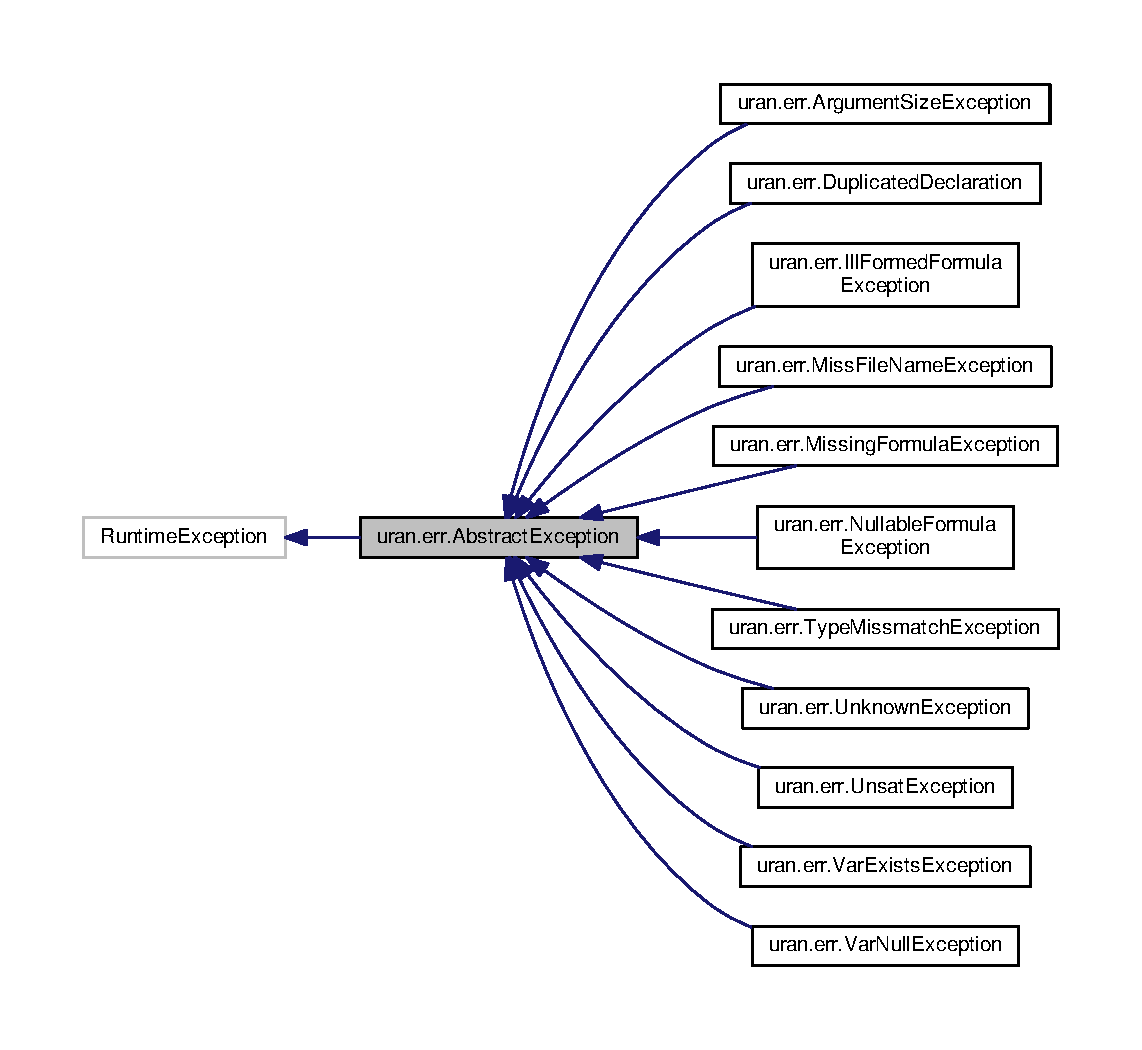
\includegraphics[width=350pt]{classuran_1_1err_1_1_abstract_exception__inherit__graph}
\end{center}
\end{figure}


Collaboration diagram for uran.\+err.\+Abstract\+Exception\+:
\nopagebreak
\begin{figure}[H]
\begin{center}
\leavevmode
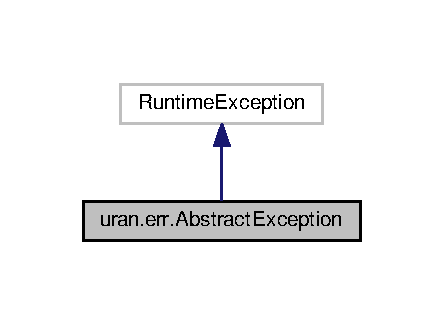
\includegraphics[width=213pt]{classuran_1_1err_1_1_abstract_exception__coll__graph}
\end{center}
\end{figure}
\subsection*{Public Member Functions}
\begin{DoxyCompactItemize}
\item 
\hyperlink{classuran_1_1err_1_1_abstract_exception_ad814ff8134a792846bdaff91f2078145}{Abstract\+Exception} ()
\item 
\hyperlink{classuran_1_1err_1_1_abstract_exception_af6af7a3d8504bd05a9364fd01188d86e}{Abstract\+Exception} (String msg)
\item 
\hyperlink{classuran_1_1err_1_1_abstract_exception_a5154c92701cc80829b6fdf5e52b2487e}{Abstract\+Exception} (String msg, int \hyperlink{classuran_1_1err_1_1_abstract_exception_ae7426fa980ba2adb26260f26f8013ee3}{code})
\end{DoxyCompactItemize}
\subsection*{Protected Attributes}
\begin{DoxyCompactItemize}
\item 
int \hyperlink{classuran_1_1err_1_1_abstract_exception_ae7426fa980ba2adb26260f26f8013ee3}{code}
\end{DoxyCompactItemize}


\subsection{Detailed Description}


Definition at line 17 of file Abstract\+Exception.\+java.



\subsection{Constructor \& Destructor Documentation}
\hypertarget{classuran_1_1err_1_1_abstract_exception_ad814ff8134a792846bdaff91f2078145}{}\index{uran\+::err\+::\+Abstract\+Exception@{uran\+::err\+::\+Abstract\+Exception}!Abstract\+Exception@{Abstract\+Exception}}
\index{Abstract\+Exception@{Abstract\+Exception}!uran\+::err\+::\+Abstract\+Exception@{uran\+::err\+::\+Abstract\+Exception}}
\subsubsection[{Abstract\+Exception}]{\setlength{\rightskip}{0pt plus 5cm}uran.\+err.\+Abstract\+Exception.\+Abstract\+Exception (
\begin{DoxyParamCaption}
{}
\end{DoxyParamCaption}
)\hspace{0.3cm}{\ttfamily [inline]}}\label{classuran_1_1err_1_1_abstract_exception_ad814ff8134a792846bdaff91f2078145}


Definition at line 23 of file Abstract\+Exception.\+java.

\hypertarget{classuran_1_1err_1_1_abstract_exception_af6af7a3d8504bd05a9364fd01188d86e}{}\index{uran\+::err\+::\+Abstract\+Exception@{uran\+::err\+::\+Abstract\+Exception}!Abstract\+Exception@{Abstract\+Exception}}
\index{Abstract\+Exception@{Abstract\+Exception}!uran\+::err\+::\+Abstract\+Exception@{uran\+::err\+::\+Abstract\+Exception}}
\subsubsection[{Abstract\+Exception}]{\setlength{\rightskip}{0pt plus 5cm}uran.\+err.\+Abstract\+Exception.\+Abstract\+Exception (
\begin{DoxyParamCaption}
\item[{String}]{msg}
\end{DoxyParamCaption}
)\hspace{0.3cm}{\ttfamily [inline]}}\label{classuran_1_1err_1_1_abstract_exception_af6af7a3d8504bd05a9364fd01188d86e}


Definition at line 25 of file Abstract\+Exception.\+java.

\hypertarget{classuran_1_1err_1_1_abstract_exception_a5154c92701cc80829b6fdf5e52b2487e}{}\index{uran\+::err\+::\+Abstract\+Exception@{uran\+::err\+::\+Abstract\+Exception}!Abstract\+Exception@{Abstract\+Exception}}
\index{Abstract\+Exception@{Abstract\+Exception}!uran\+::err\+::\+Abstract\+Exception@{uran\+::err\+::\+Abstract\+Exception}}
\subsubsection[{Abstract\+Exception}]{\setlength{\rightskip}{0pt plus 5cm}uran.\+err.\+Abstract\+Exception.\+Abstract\+Exception (
\begin{DoxyParamCaption}
\item[{String}]{msg, }
\item[{int}]{code}
\end{DoxyParamCaption}
)\hspace{0.3cm}{\ttfamily [inline]}}\label{classuran_1_1err_1_1_abstract_exception_a5154c92701cc80829b6fdf5e52b2487e}


Definition at line 27 of file Abstract\+Exception.\+java.



\subsection{Member Data Documentation}
\hypertarget{classuran_1_1err_1_1_abstract_exception_ae7426fa980ba2adb26260f26f8013ee3}{}\index{uran\+::err\+::\+Abstract\+Exception@{uran\+::err\+::\+Abstract\+Exception}!code@{code}}
\index{code@{code}!uran\+::err\+::\+Abstract\+Exception@{uran\+::err\+::\+Abstract\+Exception}}
\subsubsection[{code}]{\setlength{\rightskip}{0pt plus 5cm}int uran.\+err.\+Abstract\+Exception.\+code\hspace{0.3cm}{\ttfamily [protected]}}\label{classuran_1_1err_1_1_abstract_exception_ae7426fa980ba2adb26260f26f8013ee3}


Definition at line 20 of file Abstract\+Exception.\+java.



The documentation for this class was generated from the following file\+:\begin{DoxyCompactItemize}
\item 
/home/haowu/uran/src/uran/err/\hyperlink{_abstract_exception_8java}{Abstract\+Exception.\+java}\end{DoxyCompactItemize}

\hypertarget{classuran_1_1formula_1_1_abstract_formula}{}\section{uran.\+formula.\+Abstract\+Formula Class Reference}
\label{classuran_1_1formula_1_1_abstract_formula}\index{uran.\+formula.\+Abstract\+Formula@{uran.\+formula.\+Abstract\+Formula}}


Inheritance diagram for uran.\+formula.\+Abstract\+Formula\+:
\nopagebreak
\begin{figure}[H]
\begin{center}
\leavevmode
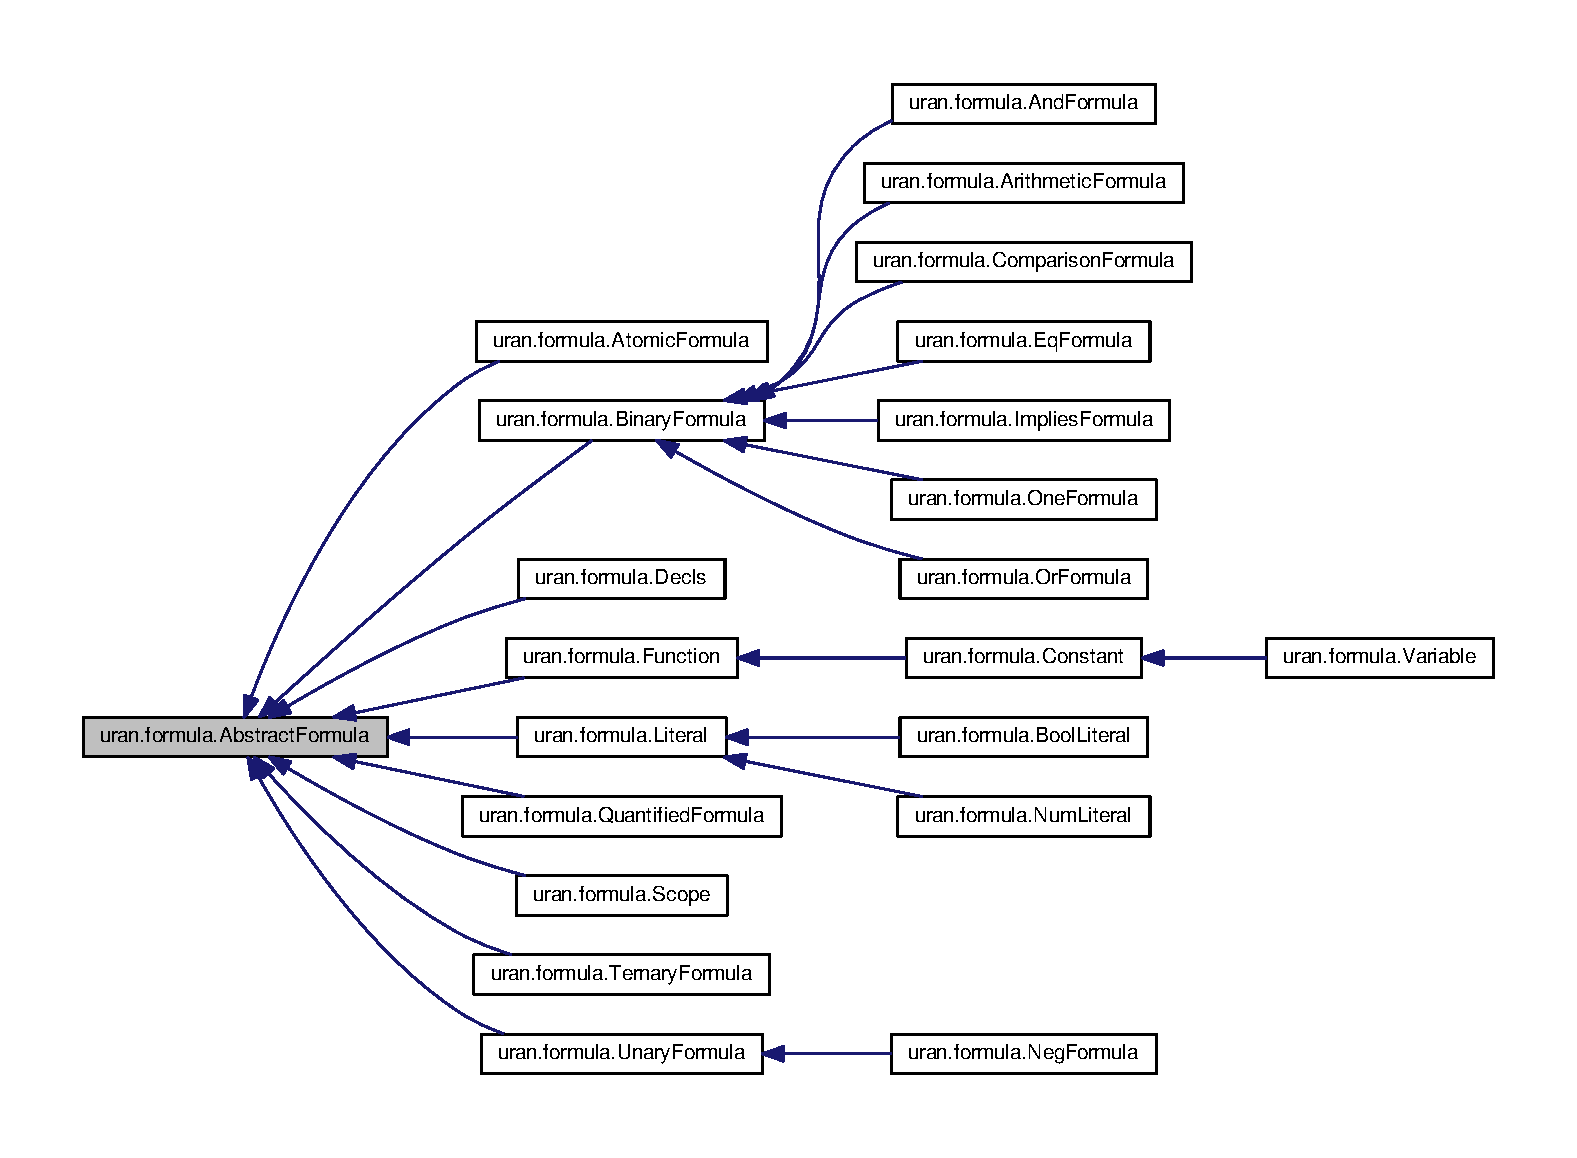
\includegraphics[width=350pt]{classuran_1_1formula_1_1_abstract_formula__inherit__graph}
\end{center}
\end{figure}
\subsection*{Public Member Functions}
\begin{DoxyCompactItemize}
\item 
abstract String \hyperlink{classuran_1_1formula_1_1_abstract_formula_a5282c2da0e6e60f04a9ec12dc464ad92}{to\+String} ()
\item 
boolean \hyperlink{classuran_1_1formula_1_1_abstract_formula_aa65d81149375ac14b5f41f0e50d958d2}{is\+Atomic\+Formula} ()
\item 
boolean \hyperlink{classuran_1_1formula_1_1_abstract_formula_aaa4108f7c1f2df24226c983427393489}{is\+Literal} ()
\item 
boolean \hyperlink{classuran_1_1formula_1_1_abstract_formula_aa3eba3be20ee0147c012ba714def29a1}{is\+Quantified\+Formula} ()
\item 
boolean \hyperlink{classuran_1_1formula_1_1_abstract_formula_a4106323335837eddb318a9c788267c68}{is\+Binary\+Formula} ()
\item 
boolean \hyperlink{classuran_1_1formula_1_1_abstract_formula_a0dc398cdff34b194567a6cb1f23e5ec2}{is\+Implies\+Formula} ()
\item 
boolean \hyperlink{classuran_1_1formula_1_1_abstract_formula_aa10fdb82bc02be16f40d749cae3b1512}{is\+Constant} ()
\item 
boolean \hyperlink{classuran_1_1formula_1_1_abstract_formula_a207a1c88a41f76f87b0dcd18a8b05110}{is\+Function} ()
\item 
boolean \hyperlink{classuran_1_1formula_1_1_abstract_formula_ad60eae4880be8f48567b7bc46e262ad5}{is\+Variable} ()
\item 
boolean \hyperlink{classuran_1_1formula_1_1_abstract_formula_ac9be0d562a154e71a1434a8778f32c90}{is\+Eq\+Formula} ()
\item 
boolean \hyperlink{classuran_1_1formula_1_1_abstract_formula_acf5976057fd55c46099706490e63f1a1}{is\+Null} ()
\item 
abstract String \hyperlink{classuran_1_1formula_1_1_abstract_formula_ac604617b889c941a8c7ef2f4afa47490}{to\+S\+M\+T2} ()
\item 
abstract void \hyperlink{classuran_1_1formula_1_1_abstract_formula_ac8fa336f6b92b478d83ec74668179da0}{accept} (\hyperlink{classuran_1_1formula_1_1visitor_1_1_abstract_visitor}{Abstract\+Visitor} visitor)
\end{DoxyCompactItemize}


\subsection{Detailed Description}
Abstract formula\+: this is the base class for all the formulas 

Definition at line 19 of file Abstract\+Formula.\+java.



\subsection{Member Function Documentation}
\hypertarget{classuran_1_1formula_1_1_abstract_formula_ac8fa336f6b92b478d83ec74668179da0}{}\index{uran\+::formula\+::\+Abstract\+Formula@{uran\+::formula\+::\+Abstract\+Formula}!accept@{accept}}
\index{accept@{accept}!uran\+::formula\+::\+Abstract\+Formula@{uran\+::formula\+::\+Abstract\+Formula}}
\subsubsection[{accept}]{\setlength{\rightskip}{0pt plus 5cm}abstract void uran.\+formula.\+Abstract\+Formula.\+accept (
\begin{DoxyParamCaption}
\item[{{\bf Abstract\+Visitor}}]{visitor}
\end{DoxyParamCaption}
)\hspace{0.3cm}{\ttfamily [abstract]}}\label{classuran_1_1formula_1_1_abstract_formula_ac8fa336f6b92b478d83ec74668179da0}
visit all nodes in a formula (visitor pattern) \hypertarget{classuran_1_1formula_1_1_abstract_formula_aa65d81149375ac14b5f41f0e50d958d2}{}\index{uran\+::formula\+::\+Abstract\+Formula@{uran\+::formula\+::\+Abstract\+Formula}!is\+Atomic\+Formula@{is\+Atomic\+Formula}}
\index{is\+Atomic\+Formula@{is\+Atomic\+Formula}!uran\+::formula\+::\+Abstract\+Formula@{uran\+::formula\+::\+Abstract\+Formula}}
\subsubsection[{is\+Atomic\+Formula}]{\setlength{\rightskip}{0pt plus 5cm}boolean uran.\+formula.\+Abstract\+Formula.\+is\+Atomic\+Formula (
\begin{DoxyParamCaption}
{}
\end{DoxyParamCaption}
)\hspace{0.3cm}{\ttfamily [inline]}}\label{classuran_1_1formula_1_1_abstract_formula_aa65d81149375ac14b5f41f0e50d958d2}


Definition at line 23 of file Abstract\+Formula.\+java.

\hypertarget{classuran_1_1formula_1_1_abstract_formula_a4106323335837eddb318a9c788267c68}{}\index{uran\+::formula\+::\+Abstract\+Formula@{uran\+::formula\+::\+Abstract\+Formula}!is\+Binary\+Formula@{is\+Binary\+Formula}}
\index{is\+Binary\+Formula@{is\+Binary\+Formula}!uran\+::formula\+::\+Abstract\+Formula@{uran\+::formula\+::\+Abstract\+Formula}}
\subsubsection[{is\+Binary\+Formula}]{\setlength{\rightskip}{0pt plus 5cm}boolean uran.\+formula.\+Abstract\+Formula.\+is\+Binary\+Formula (
\begin{DoxyParamCaption}
{}
\end{DoxyParamCaption}
)\hspace{0.3cm}{\ttfamily [inline]}}\label{classuran_1_1formula_1_1_abstract_formula_a4106323335837eddb318a9c788267c68}


Definition at line 26 of file Abstract\+Formula.\+java.

\hypertarget{classuran_1_1formula_1_1_abstract_formula_aa10fdb82bc02be16f40d749cae3b1512}{}\index{uran\+::formula\+::\+Abstract\+Formula@{uran\+::formula\+::\+Abstract\+Formula}!is\+Constant@{is\+Constant}}
\index{is\+Constant@{is\+Constant}!uran\+::formula\+::\+Abstract\+Formula@{uran\+::formula\+::\+Abstract\+Formula}}
\subsubsection[{is\+Constant}]{\setlength{\rightskip}{0pt plus 5cm}boolean uran.\+formula.\+Abstract\+Formula.\+is\+Constant (
\begin{DoxyParamCaption}
{}
\end{DoxyParamCaption}
)\hspace{0.3cm}{\ttfamily [inline]}}\label{classuran_1_1formula_1_1_abstract_formula_aa10fdb82bc02be16f40d749cae3b1512}


Definition at line 28 of file Abstract\+Formula.\+java.

\hypertarget{classuran_1_1formula_1_1_abstract_formula_ac9be0d562a154e71a1434a8778f32c90}{}\index{uran\+::formula\+::\+Abstract\+Formula@{uran\+::formula\+::\+Abstract\+Formula}!is\+Eq\+Formula@{is\+Eq\+Formula}}
\index{is\+Eq\+Formula@{is\+Eq\+Formula}!uran\+::formula\+::\+Abstract\+Formula@{uran\+::formula\+::\+Abstract\+Formula}}
\subsubsection[{is\+Eq\+Formula}]{\setlength{\rightskip}{0pt plus 5cm}boolean uran.\+formula.\+Abstract\+Formula.\+is\+Eq\+Formula (
\begin{DoxyParamCaption}
{}
\end{DoxyParamCaption}
)\hspace{0.3cm}{\ttfamily [inline]}}\label{classuran_1_1formula_1_1_abstract_formula_ac9be0d562a154e71a1434a8778f32c90}


Definition at line 31 of file Abstract\+Formula.\+java.

\hypertarget{classuran_1_1formula_1_1_abstract_formula_a207a1c88a41f76f87b0dcd18a8b05110}{}\index{uran\+::formula\+::\+Abstract\+Formula@{uran\+::formula\+::\+Abstract\+Formula}!is\+Function@{is\+Function}}
\index{is\+Function@{is\+Function}!uran\+::formula\+::\+Abstract\+Formula@{uran\+::formula\+::\+Abstract\+Formula}}
\subsubsection[{is\+Function}]{\setlength{\rightskip}{0pt plus 5cm}boolean uran.\+formula.\+Abstract\+Formula.\+is\+Function (
\begin{DoxyParamCaption}
{}
\end{DoxyParamCaption}
)\hspace{0.3cm}{\ttfamily [inline]}}\label{classuran_1_1formula_1_1_abstract_formula_a207a1c88a41f76f87b0dcd18a8b05110}


Definition at line 29 of file Abstract\+Formula.\+java.

\hypertarget{classuran_1_1formula_1_1_abstract_formula_a0dc398cdff34b194567a6cb1f23e5ec2}{}\index{uran\+::formula\+::\+Abstract\+Formula@{uran\+::formula\+::\+Abstract\+Formula}!is\+Implies\+Formula@{is\+Implies\+Formula}}
\index{is\+Implies\+Formula@{is\+Implies\+Formula}!uran\+::formula\+::\+Abstract\+Formula@{uran\+::formula\+::\+Abstract\+Formula}}
\subsubsection[{is\+Implies\+Formula}]{\setlength{\rightskip}{0pt plus 5cm}boolean uran.\+formula.\+Abstract\+Formula.\+is\+Implies\+Formula (
\begin{DoxyParamCaption}
{}
\end{DoxyParamCaption}
)\hspace{0.3cm}{\ttfamily [inline]}}\label{classuran_1_1formula_1_1_abstract_formula_a0dc398cdff34b194567a6cb1f23e5ec2}


Definition at line 27 of file Abstract\+Formula.\+java.

\hypertarget{classuran_1_1formula_1_1_abstract_formula_aaa4108f7c1f2df24226c983427393489}{}\index{uran\+::formula\+::\+Abstract\+Formula@{uran\+::formula\+::\+Abstract\+Formula}!is\+Literal@{is\+Literal}}
\index{is\+Literal@{is\+Literal}!uran\+::formula\+::\+Abstract\+Formula@{uran\+::formula\+::\+Abstract\+Formula}}
\subsubsection[{is\+Literal}]{\setlength{\rightskip}{0pt plus 5cm}boolean uran.\+formula.\+Abstract\+Formula.\+is\+Literal (
\begin{DoxyParamCaption}
{}
\end{DoxyParamCaption}
)\hspace{0.3cm}{\ttfamily [inline]}}\label{classuran_1_1formula_1_1_abstract_formula_aaa4108f7c1f2df24226c983427393489}


Definition at line 24 of file Abstract\+Formula.\+java.

\hypertarget{classuran_1_1formula_1_1_abstract_formula_acf5976057fd55c46099706490e63f1a1}{}\index{uran\+::formula\+::\+Abstract\+Formula@{uran\+::formula\+::\+Abstract\+Formula}!is\+Null@{is\+Null}}
\index{is\+Null@{is\+Null}!uran\+::formula\+::\+Abstract\+Formula@{uran\+::formula\+::\+Abstract\+Formula}}
\subsubsection[{is\+Null}]{\setlength{\rightskip}{0pt plus 5cm}boolean uran.\+formula.\+Abstract\+Formula.\+is\+Null (
\begin{DoxyParamCaption}
{}
\end{DoxyParamCaption}
)\hspace{0.3cm}{\ttfamily [inline]}}\label{classuran_1_1formula_1_1_abstract_formula_acf5976057fd55c46099706490e63f1a1}
just for the sake of inheritance 

Definition at line 34 of file Abstract\+Formula.\+java.

\hypertarget{classuran_1_1formula_1_1_abstract_formula_aa3eba3be20ee0147c012ba714def29a1}{}\index{uran\+::formula\+::\+Abstract\+Formula@{uran\+::formula\+::\+Abstract\+Formula}!is\+Quantified\+Formula@{is\+Quantified\+Formula}}
\index{is\+Quantified\+Formula@{is\+Quantified\+Formula}!uran\+::formula\+::\+Abstract\+Formula@{uran\+::formula\+::\+Abstract\+Formula}}
\subsubsection[{is\+Quantified\+Formula}]{\setlength{\rightskip}{0pt plus 5cm}boolean uran.\+formula.\+Abstract\+Formula.\+is\+Quantified\+Formula (
\begin{DoxyParamCaption}
{}
\end{DoxyParamCaption}
)\hspace{0.3cm}{\ttfamily [inline]}}\label{classuran_1_1formula_1_1_abstract_formula_aa3eba3be20ee0147c012ba714def29a1}


Definition at line 25 of file Abstract\+Formula.\+java.

\hypertarget{classuran_1_1formula_1_1_abstract_formula_ad60eae4880be8f48567b7bc46e262ad5}{}\index{uran\+::formula\+::\+Abstract\+Formula@{uran\+::formula\+::\+Abstract\+Formula}!is\+Variable@{is\+Variable}}
\index{is\+Variable@{is\+Variable}!uran\+::formula\+::\+Abstract\+Formula@{uran\+::formula\+::\+Abstract\+Formula}}
\subsubsection[{is\+Variable}]{\setlength{\rightskip}{0pt plus 5cm}boolean uran.\+formula.\+Abstract\+Formula.\+is\+Variable (
\begin{DoxyParamCaption}
{}
\end{DoxyParamCaption}
)\hspace{0.3cm}{\ttfamily [inline]}}\label{classuran_1_1formula_1_1_abstract_formula_ad60eae4880be8f48567b7bc46e262ad5}


Definition at line 30 of file Abstract\+Formula.\+java.

\hypertarget{classuran_1_1formula_1_1_abstract_formula_ac604617b889c941a8c7ef2f4afa47490}{}\index{uran\+::formula\+::\+Abstract\+Formula@{uran\+::formula\+::\+Abstract\+Formula}!to\+S\+M\+T2@{to\+S\+M\+T2}}
\index{to\+S\+M\+T2@{to\+S\+M\+T2}!uran\+::formula\+::\+Abstract\+Formula@{uran\+::formula\+::\+Abstract\+Formula}}
\subsubsection[{to\+S\+M\+T2}]{\setlength{\rightskip}{0pt plus 5cm}abstract String uran.\+formula.\+Abstract\+Formula.\+to\+S\+M\+T2 (
\begin{DoxyParamCaption}
{}
\end{DoxyParamCaption}
)\hspace{0.3cm}{\ttfamily [abstract]}}\label{classuran_1_1formula_1_1_abstract_formula_ac604617b889c941a8c7ef2f4afa47490}
output a string representation in \hyperlink{namespaceuran_1_1formula_1_1smt2}{smt2} format \hypertarget{classuran_1_1formula_1_1_abstract_formula_a5282c2da0e6e60f04a9ec12dc464ad92}{}\index{uran\+::formula\+::\+Abstract\+Formula@{uran\+::formula\+::\+Abstract\+Formula}!to\+String@{to\+String}}
\index{to\+String@{to\+String}!uran\+::formula\+::\+Abstract\+Formula@{uran\+::formula\+::\+Abstract\+Formula}}
\subsubsection[{to\+String}]{\setlength{\rightskip}{0pt plus 5cm}abstract String uran.\+formula.\+Abstract\+Formula.\+to\+String (
\begin{DoxyParamCaption}
{}
\end{DoxyParamCaption}
)\hspace{0.3cm}{\ttfamily [abstract]}}\label{classuran_1_1formula_1_1_abstract_formula_a5282c2da0e6e60f04a9ec12dc464ad92}
output a string representatino 

The documentation for this class was generated from the following file\+:\begin{DoxyCompactItemize}
\item 
/home/haowu/uran/src/uran/formula/\hyperlink{_abstract_formula_8java}{Abstract\+Formula.\+java}\end{DoxyCompactItemize}

\hypertarget{classuran_1_1formula_1_1cnf_1_1visitor_1_1_abstract_visitor}{}\section{uran.\+formula.\+cnf.\+visitor.\+Abstract\+Visitor Class Reference}
\label{classuran_1_1formula_1_1cnf_1_1visitor_1_1_abstract_visitor}\index{uran.\+formula.\+cnf.\+visitor.\+Abstract\+Visitor@{uran.\+formula.\+cnf.\+visitor.\+Abstract\+Visitor}}


Inheritance diagram for uran.\+formula.\+cnf.\+visitor.\+Abstract\+Visitor\+:
\nopagebreak
\begin{figure}[H]
\begin{center}
\leavevmode
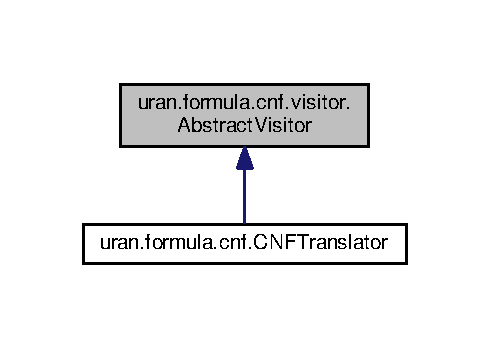
\includegraphics[width=235pt]{classuran_1_1formula_1_1cnf_1_1visitor_1_1_abstract_visitor__inherit__graph}
\end{center}
\end{figure}
\subsection*{Public Member Functions}
\begin{DoxyCompactItemize}
\item 
abstract void \hyperlink{classuran_1_1formula_1_1cnf_1_1visitor_1_1_abstract_visitor_a551b6f0af75ef93cd5b04a5488109fae}{visit} (\hyperlink{classuran_1_1formula_1_1cnf_1_1_boolean_variable}{Boolean\+Variable} v)
\item 
abstract void \hyperlink{classuran_1_1formula_1_1cnf_1_1visitor_1_1_abstract_visitor_ab7c9d906d3da6675a91bad079e193c78}{visit} (\hyperlink{classuran_1_1formula_1_1cnf_1_1_binary_gate}{Binary\+Gate} b)
\item 
abstract void \hyperlink{classuran_1_1formula_1_1cnf_1_1visitor_1_1_abstract_visitor_a1ff0fc0dfb5ea14efa693009f3954ce4}{visit} (\hyperlink{classuran_1_1formula_1_1cnf_1_1_not_gate}{Not\+Gate} n)
\end{DoxyCompactItemize}


\subsection{Detailed Description}


Definition at line 19 of file Abstract\+Visitor.\+java.



\subsection{Member Function Documentation}
\hypertarget{classuran_1_1formula_1_1cnf_1_1visitor_1_1_abstract_visitor_a551b6f0af75ef93cd5b04a5488109fae}{}\index{uran\+::formula\+::cnf\+::visitor\+::\+Abstract\+Visitor@{uran\+::formula\+::cnf\+::visitor\+::\+Abstract\+Visitor}!visit@{visit}}
\index{visit@{visit}!uran\+::formula\+::cnf\+::visitor\+::\+Abstract\+Visitor@{uran\+::formula\+::cnf\+::visitor\+::\+Abstract\+Visitor}}
\subsubsection[{visit}]{\setlength{\rightskip}{0pt plus 5cm}abstract void uran.\+formula.\+cnf.\+visitor.\+Abstract\+Visitor.\+visit (
\begin{DoxyParamCaption}
\item[{{\bf Boolean\+Variable}}]{v}
\end{DoxyParamCaption}
)\hspace{0.3cm}{\ttfamily [abstract]}}\label{classuran_1_1formula_1_1cnf_1_1visitor_1_1_abstract_visitor_a551b6f0af75ef93cd5b04a5488109fae}
\hypertarget{classuran_1_1formula_1_1cnf_1_1visitor_1_1_abstract_visitor_ab7c9d906d3da6675a91bad079e193c78}{}\index{uran\+::formula\+::cnf\+::visitor\+::\+Abstract\+Visitor@{uran\+::formula\+::cnf\+::visitor\+::\+Abstract\+Visitor}!visit@{visit}}
\index{visit@{visit}!uran\+::formula\+::cnf\+::visitor\+::\+Abstract\+Visitor@{uran\+::formula\+::cnf\+::visitor\+::\+Abstract\+Visitor}}
\subsubsection[{visit}]{\setlength{\rightskip}{0pt plus 5cm}abstract void uran.\+formula.\+cnf.\+visitor.\+Abstract\+Visitor.\+visit (
\begin{DoxyParamCaption}
\item[{{\bf Binary\+Gate}}]{b}
\end{DoxyParamCaption}
)\hspace{0.3cm}{\ttfamily [abstract]}}\label{classuran_1_1formula_1_1cnf_1_1visitor_1_1_abstract_visitor_ab7c9d906d3da6675a91bad079e193c78}
\hypertarget{classuran_1_1formula_1_1cnf_1_1visitor_1_1_abstract_visitor_a1ff0fc0dfb5ea14efa693009f3954ce4}{}\index{uran\+::formula\+::cnf\+::visitor\+::\+Abstract\+Visitor@{uran\+::formula\+::cnf\+::visitor\+::\+Abstract\+Visitor}!visit@{visit}}
\index{visit@{visit}!uran\+::formula\+::cnf\+::visitor\+::\+Abstract\+Visitor@{uran\+::formula\+::cnf\+::visitor\+::\+Abstract\+Visitor}}
\subsubsection[{visit}]{\setlength{\rightskip}{0pt plus 5cm}abstract void uran.\+formula.\+cnf.\+visitor.\+Abstract\+Visitor.\+visit (
\begin{DoxyParamCaption}
\item[{{\bf Not\+Gate}}]{n}
\end{DoxyParamCaption}
)\hspace{0.3cm}{\ttfamily [abstract]}}\label{classuran_1_1formula_1_1cnf_1_1visitor_1_1_abstract_visitor_a1ff0fc0dfb5ea14efa693009f3954ce4}


The documentation for this class was generated from the following file\+:\begin{DoxyCompactItemize}
\item 
/home/haowu/uran/src/uran/formula/cnf/visitor/\hyperlink{cnf_2visitor_2_abstract_visitor_8java}{Abstract\+Visitor.\+java}\end{DoxyCompactItemize}

\hypertarget{classuran_1_1formula_1_1visitor_1_1_abstract_visitor}{}\section{uran.\+formula.\+visitor.\+Abstract\+Visitor Class Reference}
\label{classuran_1_1formula_1_1visitor_1_1_abstract_visitor}\index{uran.\+formula.\+visitor.\+Abstract\+Visitor@{uran.\+formula.\+visitor.\+Abstract\+Visitor}}


Inheritance diagram for uran.\+formula.\+visitor.\+Abstract\+Visitor\+:
\nopagebreak
\begin{figure}[H]
\begin{center}
\leavevmode
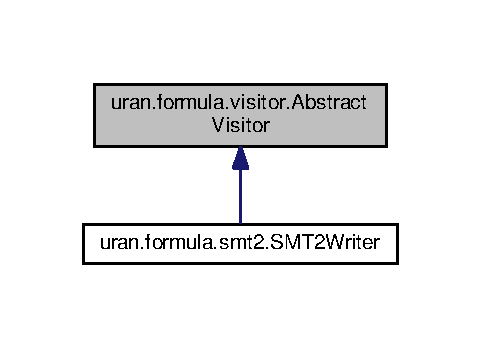
\includegraphics[width=231pt]{classuran_1_1formula_1_1visitor_1_1_abstract_visitor__inherit__graph}
\end{center}
\end{figure}
\subsection*{Public Member Functions}
\begin{DoxyCompactItemize}
\item 
abstract void \hyperlink{classuran_1_1formula_1_1visitor_1_1_abstract_visitor_ae1d53ba07e557623193ae83780fbb7da}{visit} (\hyperlink{classuran_1_1formula_1_1_binary_formula}{Binary\+Formula} f)
\item 
abstract void \hyperlink{classuran_1_1formula_1_1visitor_1_1_abstract_visitor_a3187c0eac87e1d1e168dac4c4afb9ffd}{visit} (\hyperlink{classuran_1_1formula_1_1_implies_formula}{Implies\+Formula} f)
\item 
abstract void \hyperlink{classuran_1_1formula_1_1visitor_1_1_abstract_visitor_a98e90c05d16923d77a97136e0227d65e}{visit} (\hyperlink{classuran_1_1formula_1_1_neg_formula}{Neg\+Formula} f)
\item 
abstract void \hyperlink{classuran_1_1formula_1_1visitor_1_1_abstract_visitor_a77a85766b6d9e1d56db93debe3f1c7b7}{visit} (\hyperlink{classuran_1_1formula_1_1_function}{Function} f)
\item 
abstract void \hyperlink{classuran_1_1formula_1_1visitor_1_1_abstract_visitor_a2a0b836e52b91d5b7076eda3f945a5f5}{visit} (\hyperlink{classuran_1_1formula_1_1_quantified_formula}{Quantified\+Formula} f)
\item 
abstract void \hyperlink{classuran_1_1formula_1_1visitor_1_1_abstract_visitor_afa870c96cefdddb436fcdf22e006d14d}{visit} (\hyperlink{classuran_1_1formula_1_1_scope}{Scope} s)
\item 
abstract void \hyperlink{classuran_1_1formula_1_1visitor_1_1_abstract_visitor_aa53c4043c10971de2f3fba19d25b74a8}{visit} (\hyperlink{classuran_1_1formula_1_1_decls}{Decls} d)
\item 
abstract void \hyperlink{classuran_1_1formula_1_1visitor_1_1_abstract_visitor_ac4da59daf9cda9e46e8f8f018c46c3ce}{visit} (\hyperlink{classuran_1_1formula_1_1_bool_literal}{Bool\+Literal} l)
\item 
abstract void \hyperlink{classuran_1_1formula_1_1visitor_1_1_abstract_visitor_a81a183cdcb00d078c86154e2b4662caa}{visit} (\hyperlink{classuran_1_1formula_1_1_num_literal}{Num\+Literal} l)
\end{DoxyCompactItemize}


\subsection{Detailed Description}


Definition at line 19 of file Abstract\+Visitor.\+java.



\subsection{Member Function Documentation}
\hypertarget{classuran_1_1formula_1_1visitor_1_1_abstract_visitor_ae1d53ba07e557623193ae83780fbb7da}{}\index{uran\+::formula\+::visitor\+::\+Abstract\+Visitor@{uran\+::formula\+::visitor\+::\+Abstract\+Visitor}!visit@{visit}}
\index{visit@{visit}!uran\+::formula\+::visitor\+::\+Abstract\+Visitor@{uran\+::formula\+::visitor\+::\+Abstract\+Visitor}}
\subsubsection[{visit}]{\setlength{\rightskip}{0pt plus 5cm}abstract void uran.\+formula.\+visitor.\+Abstract\+Visitor.\+visit (
\begin{DoxyParamCaption}
\item[{{\bf Binary\+Formula}}]{f}
\end{DoxyParamCaption}
)\hspace{0.3cm}{\ttfamily [abstract]}}\label{classuran_1_1formula_1_1visitor_1_1_abstract_visitor_ae1d53ba07e557623193ae83780fbb7da}
\hypertarget{classuran_1_1formula_1_1visitor_1_1_abstract_visitor_a3187c0eac87e1d1e168dac4c4afb9ffd}{}\index{uran\+::formula\+::visitor\+::\+Abstract\+Visitor@{uran\+::formula\+::visitor\+::\+Abstract\+Visitor}!visit@{visit}}
\index{visit@{visit}!uran\+::formula\+::visitor\+::\+Abstract\+Visitor@{uran\+::formula\+::visitor\+::\+Abstract\+Visitor}}
\subsubsection[{visit}]{\setlength{\rightskip}{0pt plus 5cm}abstract void uran.\+formula.\+visitor.\+Abstract\+Visitor.\+visit (
\begin{DoxyParamCaption}
\item[{{\bf Implies\+Formula}}]{f}
\end{DoxyParamCaption}
)\hspace{0.3cm}{\ttfamily [abstract]}}\label{classuran_1_1formula_1_1visitor_1_1_abstract_visitor_a3187c0eac87e1d1e168dac4c4afb9ffd}
\hypertarget{classuran_1_1formula_1_1visitor_1_1_abstract_visitor_a98e90c05d16923d77a97136e0227d65e}{}\index{uran\+::formula\+::visitor\+::\+Abstract\+Visitor@{uran\+::formula\+::visitor\+::\+Abstract\+Visitor}!visit@{visit}}
\index{visit@{visit}!uran\+::formula\+::visitor\+::\+Abstract\+Visitor@{uran\+::formula\+::visitor\+::\+Abstract\+Visitor}}
\subsubsection[{visit}]{\setlength{\rightskip}{0pt plus 5cm}abstract void uran.\+formula.\+visitor.\+Abstract\+Visitor.\+visit (
\begin{DoxyParamCaption}
\item[{{\bf Neg\+Formula}}]{f}
\end{DoxyParamCaption}
)\hspace{0.3cm}{\ttfamily [abstract]}}\label{classuran_1_1formula_1_1visitor_1_1_abstract_visitor_a98e90c05d16923d77a97136e0227d65e}
\hypertarget{classuran_1_1formula_1_1visitor_1_1_abstract_visitor_a77a85766b6d9e1d56db93debe3f1c7b7}{}\index{uran\+::formula\+::visitor\+::\+Abstract\+Visitor@{uran\+::formula\+::visitor\+::\+Abstract\+Visitor}!visit@{visit}}
\index{visit@{visit}!uran\+::formula\+::visitor\+::\+Abstract\+Visitor@{uran\+::formula\+::visitor\+::\+Abstract\+Visitor}}
\subsubsection[{visit}]{\setlength{\rightskip}{0pt plus 5cm}abstract void uran.\+formula.\+visitor.\+Abstract\+Visitor.\+visit (
\begin{DoxyParamCaption}
\item[{{\bf Function}}]{f}
\end{DoxyParamCaption}
)\hspace{0.3cm}{\ttfamily [abstract]}}\label{classuran_1_1formula_1_1visitor_1_1_abstract_visitor_a77a85766b6d9e1d56db93debe3f1c7b7}
\hypertarget{classuran_1_1formula_1_1visitor_1_1_abstract_visitor_a2a0b836e52b91d5b7076eda3f945a5f5}{}\index{uran\+::formula\+::visitor\+::\+Abstract\+Visitor@{uran\+::formula\+::visitor\+::\+Abstract\+Visitor}!visit@{visit}}
\index{visit@{visit}!uran\+::formula\+::visitor\+::\+Abstract\+Visitor@{uran\+::formula\+::visitor\+::\+Abstract\+Visitor}}
\subsubsection[{visit}]{\setlength{\rightskip}{0pt plus 5cm}abstract void uran.\+formula.\+visitor.\+Abstract\+Visitor.\+visit (
\begin{DoxyParamCaption}
\item[{{\bf Quantified\+Formula}}]{f}
\end{DoxyParamCaption}
)\hspace{0.3cm}{\ttfamily [abstract]}}\label{classuran_1_1formula_1_1visitor_1_1_abstract_visitor_a2a0b836e52b91d5b7076eda3f945a5f5}
\hypertarget{classuran_1_1formula_1_1visitor_1_1_abstract_visitor_afa870c96cefdddb436fcdf22e006d14d}{}\index{uran\+::formula\+::visitor\+::\+Abstract\+Visitor@{uran\+::formula\+::visitor\+::\+Abstract\+Visitor}!visit@{visit}}
\index{visit@{visit}!uran\+::formula\+::visitor\+::\+Abstract\+Visitor@{uran\+::formula\+::visitor\+::\+Abstract\+Visitor}}
\subsubsection[{visit}]{\setlength{\rightskip}{0pt plus 5cm}abstract void uran.\+formula.\+visitor.\+Abstract\+Visitor.\+visit (
\begin{DoxyParamCaption}
\item[{{\bf Scope}}]{s}
\end{DoxyParamCaption}
)\hspace{0.3cm}{\ttfamily [abstract]}}\label{classuran_1_1formula_1_1visitor_1_1_abstract_visitor_afa870c96cefdddb436fcdf22e006d14d}
\hypertarget{classuran_1_1formula_1_1visitor_1_1_abstract_visitor_aa53c4043c10971de2f3fba19d25b74a8}{}\index{uran\+::formula\+::visitor\+::\+Abstract\+Visitor@{uran\+::formula\+::visitor\+::\+Abstract\+Visitor}!visit@{visit}}
\index{visit@{visit}!uran\+::formula\+::visitor\+::\+Abstract\+Visitor@{uran\+::formula\+::visitor\+::\+Abstract\+Visitor}}
\subsubsection[{visit}]{\setlength{\rightskip}{0pt plus 5cm}abstract void uran.\+formula.\+visitor.\+Abstract\+Visitor.\+visit (
\begin{DoxyParamCaption}
\item[{{\bf Decls}}]{d}
\end{DoxyParamCaption}
)\hspace{0.3cm}{\ttfamily [abstract]}}\label{classuran_1_1formula_1_1visitor_1_1_abstract_visitor_aa53c4043c10971de2f3fba19d25b74a8}
\hypertarget{classuran_1_1formula_1_1visitor_1_1_abstract_visitor_ac4da59daf9cda9e46e8f8f018c46c3ce}{}\index{uran\+::formula\+::visitor\+::\+Abstract\+Visitor@{uran\+::formula\+::visitor\+::\+Abstract\+Visitor}!visit@{visit}}
\index{visit@{visit}!uran\+::formula\+::visitor\+::\+Abstract\+Visitor@{uran\+::formula\+::visitor\+::\+Abstract\+Visitor}}
\subsubsection[{visit}]{\setlength{\rightskip}{0pt plus 5cm}abstract void uran.\+formula.\+visitor.\+Abstract\+Visitor.\+visit (
\begin{DoxyParamCaption}
\item[{{\bf Bool\+Literal}}]{l}
\end{DoxyParamCaption}
)\hspace{0.3cm}{\ttfamily [abstract]}}\label{classuran_1_1formula_1_1visitor_1_1_abstract_visitor_ac4da59daf9cda9e46e8f8f018c46c3ce}
\hypertarget{classuran_1_1formula_1_1visitor_1_1_abstract_visitor_a81a183cdcb00d078c86154e2b4662caa}{}\index{uran\+::formula\+::visitor\+::\+Abstract\+Visitor@{uran\+::formula\+::visitor\+::\+Abstract\+Visitor}!visit@{visit}}
\index{visit@{visit}!uran\+::formula\+::visitor\+::\+Abstract\+Visitor@{uran\+::formula\+::visitor\+::\+Abstract\+Visitor}}
\subsubsection[{visit}]{\setlength{\rightskip}{0pt plus 5cm}abstract void uran.\+formula.\+visitor.\+Abstract\+Visitor.\+visit (
\begin{DoxyParamCaption}
\item[{{\bf Num\+Literal}}]{l}
\end{DoxyParamCaption}
)\hspace{0.3cm}{\ttfamily [abstract]}}\label{classuran_1_1formula_1_1visitor_1_1_abstract_visitor_a81a183cdcb00d078c86154e2b4662caa}


The documentation for this class was generated from the following file\+:\begin{DoxyCompactItemize}
\item 
/home/haowu/uran/src/uran/formula/visitor/\hyperlink{visitor_2_abstract_visitor_8java}{Abstract\+Visitor.\+java}\end{DoxyCompactItemize}

\hypertarget{classuran_1_1formula_1_1_and_formula}{}\section{uran.\+formula.\+And\+Formula Class Reference}
\label{classuran_1_1formula_1_1_and_formula}\index{uran.\+formula.\+And\+Formula@{uran.\+formula.\+And\+Formula}}


Inheritance diagram for uran.\+formula.\+And\+Formula\+:
\nopagebreak
\begin{figure}[H]
\begin{center}
\leavevmode
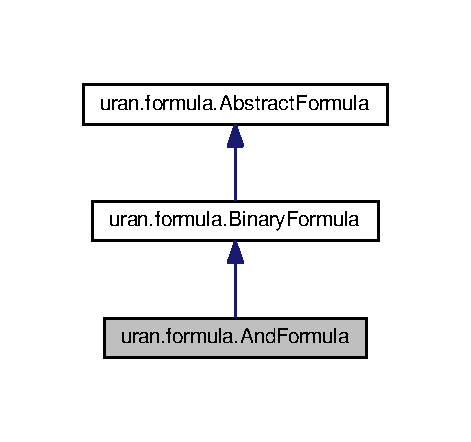
\includegraphics[width=226pt]{classuran_1_1formula_1_1_and_formula__inherit__graph}
\end{center}
\end{figure}


Collaboration diagram for uran.\+formula.\+And\+Formula\+:
\nopagebreak
\begin{figure}[H]
\begin{center}
\leavevmode
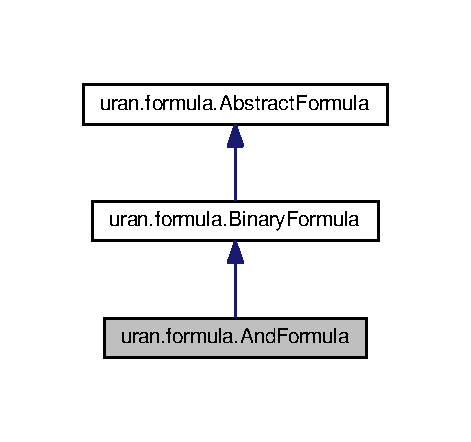
\includegraphics[width=226pt]{classuran_1_1formula_1_1_and_formula__coll__graph}
\end{center}
\end{figure}
\subsection*{Public Member Functions}
\begin{DoxyCompactItemize}
\item 
\hyperlink{classuran_1_1formula_1_1_and_formula_ab7d4dda48fd5e6f3786ad2a73b27f847}{And\+Formula} ()
\item 
\hyperlink{classuran_1_1formula_1_1_and_formula_a637456253ba7f21a91f7b0edf2fdf9a3}{And\+Formula} (\hyperlink{classuran_1_1formula_1_1_abstract_formula}{Abstract\+Formula} f1, \hyperlink{classuran_1_1formula_1_1_abstract_formula}{Abstract\+Formula} f2)
\item 
\hyperlink{classuran_1_1formula_1_1_binary_formula}{Binary\+Formula} \hyperlink{classuran_1_1formula_1_1_and_formula_a7f46ee1f0d9c15d2f7ece35193ccf070}{merge} (Abstract\+Formula...\+formulas)
\end{DoxyCompactItemize}


\subsection{Detailed Description}
Constrcut and formula. \begin{DoxyAuthor}{Author}
Hao Wu 
\end{DoxyAuthor}


Definition at line 24 of file And\+Formula.\+java.



\subsection{Constructor \& Destructor Documentation}
\hypertarget{classuran_1_1formula_1_1_and_formula_ab7d4dda48fd5e6f3786ad2a73b27f847}{}\index{uran\+::formula\+::\+And\+Formula@{uran\+::formula\+::\+And\+Formula}!And\+Formula@{And\+Formula}}
\index{And\+Formula@{And\+Formula}!uran\+::formula\+::\+And\+Formula@{uran\+::formula\+::\+And\+Formula}}
\subsubsection[{And\+Formula}]{\setlength{\rightskip}{0pt plus 5cm}uran.\+formula.\+And\+Formula.\+And\+Formula (
\begin{DoxyParamCaption}
{}
\end{DoxyParamCaption}
)\hspace{0.3cm}{\ttfamily [inline]}}\label{classuran_1_1formula_1_1_and_formula_ab7d4dda48fd5e6f3786ad2a73b27f847}


Definition at line 25 of file And\+Formula.\+java.

\hypertarget{classuran_1_1formula_1_1_and_formula_a637456253ba7f21a91f7b0edf2fdf9a3}{}\index{uran\+::formula\+::\+And\+Formula@{uran\+::formula\+::\+And\+Formula}!And\+Formula@{And\+Formula}}
\index{And\+Formula@{And\+Formula}!uran\+::formula\+::\+And\+Formula@{uran\+::formula\+::\+And\+Formula}}
\subsubsection[{And\+Formula}]{\setlength{\rightskip}{0pt plus 5cm}uran.\+formula.\+And\+Formula.\+And\+Formula (
\begin{DoxyParamCaption}
\item[{{\bf Abstract\+Formula}}]{f1, }
\item[{{\bf Abstract\+Formula}}]{f2}
\end{DoxyParamCaption}
)\hspace{0.3cm}{\ttfamily [inline]}}\label{classuran_1_1formula_1_1_and_formula_a637456253ba7f21a91f7b0edf2fdf9a3}


Definition at line 27 of file And\+Formula.\+java.



\subsection{Member Function Documentation}
\hypertarget{classuran_1_1formula_1_1_and_formula_a7f46ee1f0d9c15d2f7ece35193ccf070}{}\index{uran\+::formula\+::\+And\+Formula@{uran\+::formula\+::\+And\+Formula}!merge@{merge}}
\index{merge@{merge}!uran\+::formula\+::\+And\+Formula@{uran\+::formula\+::\+And\+Formula}}
\subsubsection[{merge}]{\setlength{\rightskip}{0pt plus 5cm}{\bf Binary\+Formula} uran.\+formula.\+And\+Formula.\+merge (
\begin{DoxyParamCaption}
\item[{Abstract\+Formula...}]{formulas}
\end{DoxyParamCaption}
)\hspace{0.3cm}{\ttfamily [inline]}}\label{classuran_1_1formula_1_1_and_formula_a7f46ee1f0d9c15d2f7ece35193ccf070}
merge a list of formulas, all with the and gate 
\begin{DoxyParams}{Parameters}
{\em formulas} & a list of formulas. \\
\hline
\end{DoxyParams}
\begin{DoxyReturn}{Returns}
a new and formula. 
\end{DoxyReturn}


Definition at line 39 of file And\+Formula.\+java.



The documentation for this class was generated from the following file\+:\begin{DoxyCompactItemize}
\item 
/home/haowu/uran/src/uran/formula/\hyperlink{_and_formula_8java}{And\+Formula.\+java}\end{DoxyCompactItemize}

\hypertarget{classuran_1_1err_1_1_argument_size_exception}{}\section{uran.\+err.\+Argument\+Size\+Exception Class Reference}
\label{classuran_1_1err_1_1_argument_size_exception}\index{uran.\+err.\+Argument\+Size\+Exception@{uran.\+err.\+Argument\+Size\+Exception}}


Inheritance diagram for uran.\+err.\+Argument\+Size\+Exception\+:
\nopagebreak
\begin{figure}[H]
\begin{center}
\leavevmode
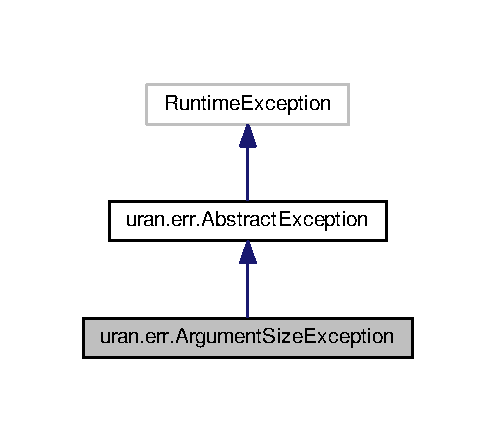
\includegraphics[width=238pt]{classuran_1_1err_1_1_argument_size_exception__inherit__graph}
\end{center}
\end{figure}


Collaboration diagram for uran.\+err.\+Argument\+Size\+Exception\+:
\nopagebreak
\begin{figure}[H]
\begin{center}
\leavevmode
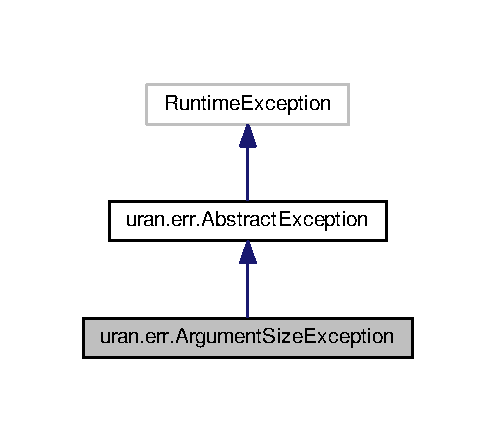
\includegraphics[width=238pt]{classuran_1_1err_1_1_argument_size_exception__coll__graph}
\end{center}
\end{figure}
\subsection*{Public Member Functions}
\begin{DoxyCompactItemize}
\item 
\hyperlink{classuran_1_1err_1_1_argument_size_exception_ae74b8113ab87a7098b1817db5c154d16}{Argument\+Size\+Exception} ()
\item 
\hyperlink{classuran_1_1err_1_1_argument_size_exception_a400a78b4a66f57e9b98aabb861c5c8a4}{Argument\+Size\+Exception} (String msg)
\end{DoxyCompactItemize}
\subsection*{Additional Inherited Members}


\subsection{Detailed Description}


Definition at line 17 of file Argument\+Size\+Exception.\+java.



\subsection{Constructor \& Destructor Documentation}
\hypertarget{classuran_1_1err_1_1_argument_size_exception_ae74b8113ab87a7098b1817db5c154d16}{}\index{uran\+::err\+::\+Argument\+Size\+Exception@{uran\+::err\+::\+Argument\+Size\+Exception}!Argument\+Size\+Exception@{Argument\+Size\+Exception}}
\index{Argument\+Size\+Exception@{Argument\+Size\+Exception}!uran\+::err\+::\+Argument\+Size\+Exception@{uran\+::err\+::\+Argument\+Size\+Exception}}
\subsubsection[{Argument\+Size\+Exception}]{\setlength{\rightskip}{0pt plus 5cm}uran.\+err.\+Argument\+Size\+Exception.\+Argument\+Size\+Exception (
\begin{DoxyParamCaption}
{}
\end{DoxyParamCaption}
)\hspace{0.3cm}{\ttfamily [inline]}}\label{classuran_1_1err_1_1_argument_size_exception_ae74b8113ab87a7098b1817db5c154d16}


Definition at line 19 of file Argument\+Size\+Exception.\+java.

\hypertarget{classuran_1_1err_1_1_argument_size_exception_a400a78b4a66f57e9b98aabb861c5c8a4}{}\index{uran\+::err\+::\+Argument\+Size\+Exception@{uran\+::err\+::\+Argument\+Size\+Exception}!Argument\+Size\+Exception@{Argument\+Size\+Exception}}
\index{Argument\+Size\+Exception@{Argument\+Size\+Exception}!uran\+::err\+::\+Argument\+Size\+Exception@{uran\+::err\+::\+Argument\+Size\+Exception}}
\subsubsection[{Argument\+Size\+Exception}]{\setlength{\rightskip}{0pt plus 5cm}uran.\+err.\+Argument\+Size\+Exception.\+Argument\+Size\+Exception (
\begin{DoxyParamCaption}
\item[{String}]{msg}
\end{DoxyParamCaption}
)\hspace{0.3cm}{\ttfamily [inline]}}\label{classuran_1_1err_1_1_argument_size_exception_a400a78b4a66f57e9b98aabb861c5c8a4}


Definition at line 24 of file Argument\+Size\+Exception.\+java.



The documentation for this class was generated from the following file\+:\begin{DoxyCompactItemize}
\item 
/home/haowu/uran/src/uran/err/\hyperlink{_argument_size_exception_8java}{Argument\+Size\+Exception.\+java}\end{DoxyCompactItemize}

\hypertarget{classuran_1_1formula_1_1_arithmetic_formula}{}\section{uran.\+formula.\+Arithmetic\+Formula Class Reference}
\label{classuran_1_1formula_1_1_arithmetic_formula}\index{uran.\+formula.\+Arithmetic\+Formula@{uran.\+formula.\+Arithmetic\+Formula}}


Inheritance diagram for uran.\+formula.\+Arithmetic\+Formula\+:
\nopagebreak
\begin{figure}[H]
\begin{center}
\leavevmode
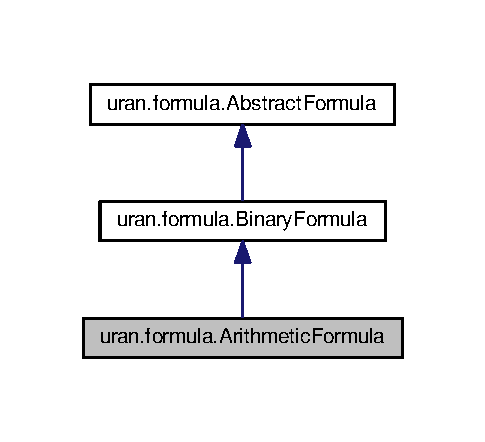
\includegraphics[width=233pt]{classuran_1_1formula_1_1_arithmetic_formula__inherit__graph}
\end{center}
\end{figure}


Collaboration diagram for uran.\+formula.\+Arithmetic\+Formula\+:
\nopagebreak
\begin{figure}[H]
\begin{center}
\leavevmode
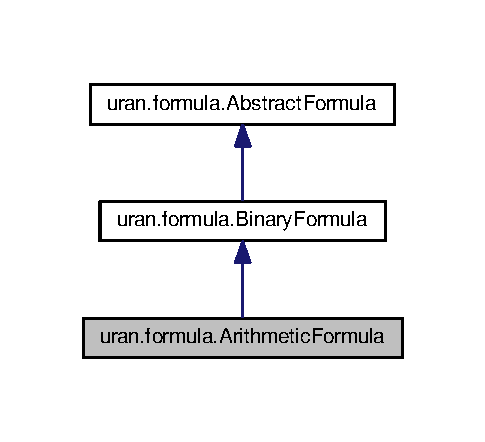
\includegraphics[width=233pt]{classuran_1_1formula_1_1_arithmetic_formula__coll__graph}
\end{center}
\end{figure}
\subsection*{Public Member Functions}
\begin{DoxyCompactItemize}
\item 
\hyperlink{classuran_1_1formula_1_1_arithmetic_formula_ad16dc08377d56c904e464e0f1a662c6c}{Arithmetic\+Formula} (\hyperlink{enumuran_1_1formula_1_1_connective}{Connective} con)
\item 
\hyperlink{classuran_1_1formula_1_1_arithmetic_formula_a4ab2a434348426fad0686b04a36f0623}{Arithmetic\+Formula} (\hyperlink{enumuran_1_1formula_1_1_connective}{Connective} con, \hyperlink{classuran_1_1formula_1_1_abstract_formula}{Abstract\+Formula} f1, \hyperlink{classuran_1_1formula_1_1_abstract_formula}{Abstract\+Formula} f2)
\item 
void \hyperlink{classuran_1_1formula_1_1_arithmetic_formula_a3e0ab4cf42a4d30d867f8b519b6d6612}{set\+Connective} (\hyperlink{enumuran_1_1formula_1_1_connective}{Connective} con)
\item 
\hyperlink{classuran_1_1formula_1_1_binary_formula}{Binary\+Formula} \hyperlink{classuran_1_1formula_1_1_arithmetic_formula_a5608bbe3e1df0775dbcedc9448b0f9d5}{merge} (Abstract\+Formula...\+formulas)
\end{DoxyCompactItemize}


\subsection{Detailed Description}
Constrcut an arithmetic formula (+,-\/,$\ast$,div) \begin{DoxyAuthor}{Author}
Hao Wu 
\end{DoxyAuthor}


Definition at line 24 of file Arithmetic\+Formula.\+java.



\subsection{Constructor \& Destructor Documentation}
\hypertarget{classuran_1_1formula_1_1_arithmetic_formula_ad16dc08377d56c904e464e0f1a662c6c}{}\index{uran\+::formula\+::\+Arithmetic\+Formula@{uran\+::formula\+::\+Arithmetic\+Formula}!Arithmetic\+Formula@{Arithmetic\+Formula}}
\index{Arithmetic\+Formula@{Arithmetic\+Formula}!uran\+::formula\+::\+Arithmetic\+Formula@{uran\+::formula\+::\+Arithmetic\+Formula}}
\subsubsection[{Arithmetic\+Formula}]{\setlength{\rightskip}{0pt plus 5cm}uran.\+formula.\+Arithmetic\+Formula.\+Arithmetic\+Formula (
\begin{DoxyParamCaption}
\item[{{\bf Connective}}]{con}
\end{DoxyParamCaption}
)\hspace{0.3cm}{\ttfamily [inline]}}\label{classuran_1_1formula_1_1_arithmetic_formula_ad16dc08377d56c904e464e0f1a662c6c}


Definition at line 25 of file Arithmetic\+Formula.\+java.

\hypertarget{classuran_1_1formula_1_1_arithmetic_formula_a4ab2a434348426fad0686b04a36f0623}{}\index{uran\+::formula\+::\+Arithmetic\+Formula@{uran\+::formula\+::\+Arithmetic\+Formula}!Arithmetic\+Formula@{Arithmetic\+Formula}}
\index{Arithmetic\+Formula@{Arithmetic\+Formula}!uran\+::formula\+::\+Arithmetic\+Formula@{uran\+::formula\+::\+Arithmetic\+Formula}}
\subsubsection[{Arithmetic\+Formula}]{\setlength{\rightskip}{0pt plus 5cm}uran.\+formula.\+Arithmetic\+Formula.\+Arithmetic\+Formula (
\begin{DoxyParamCaption}
\item[{{\bf Connective}}]{con, }
\item[{{\bf Abstract\+Formula}}]{f1, }
\item[{{\bf Abstract\+Formula}}]{f2}
\end{DoxyParamCaption}
)\hspace{0.3cm}{\ttfamily [inline]}}\label{classuran_1_1formula_1_1_arithmetic_formula_a4ab2a434348426fad0686b04a36f0623}


Definition at line 27 of file Arithmetic\+Formula.\+java.



\subsection{Member Function Documentation}
\hypertarget{classuran_1_1formula_1_1_arithmetic_formula_a5608bbe3e1df0775dbcedc9448b0f9d5}{}\index{uran\+::formula\+::\+Arithmetic\+Formula@{uran\+::formula\+::\+Arithmetic\+Formula}!merge@{merge}}
\index{merge@{merge}!uran\+::formula\+::\+Arithmetic\+Formula@{uran\+::formula\+::\+Arithmetic\+Formula}}
\subsubsection[{merge}]{\setlength{\rightskip}{0pt plus 5cm}{\bf Binary\+Formula} uran.\+formula.\+Arithmetic\+Formula.\+merge (
\begin{DoxyParamCaption}
\item[{Abstract\+Formula...}]{formulas}
\end{DoxyParamCaption}
)\hspace{0.3cm}{\ttfamily [inline]}}\label{classuran_1_1formula_1_1_arithmetic_formula_a5608bbe3e1df0775dbcedc9448b0f9d5}
merge a list of formulas 
\begin{DoxyParams}{Parameters}
{\em formulas} & list of formulas to be merged. \+: need to connect all them with A\+N\+D gates \\
\hline
\end{DoxyParams}


Definition at line 61 of file Arithmetic\+Formula.\+java.

\hypertarget{classuran_1_1formula_1_1_arithmetic_formula_a3e0ab4cf42a4d30d867f8b519b6d6612}{}\index{uran\+::formula\+::\+Arithmetic\+Formula@{uran\+::formula\+::\+Arithmetic\+Formula}!set\+Connective@{set\+Connective}}
\index{set\+Connective@{set\+Connective}!uran\+::formula\+::\+Arithmetic\+Formula@{uran\+::formula\+::\+Arithmetic\+Formula}}
\subsubsection[{set\+Connective}]{\setlength{\rightskip}{0pt plus 5cm}void uran.\+formula.\+Arithmetic\+Formula.\+set\+Connective (
\begin{DoxyParamCaption}
\item[{{\bf Connective}}]{con}
\end{DoxyParamCaption}
)\hspace{0.3cm}{\ttfamily [inline]}}\label{classuran_1_1formula_1_1_arithmetic_formula_a3e0ab4cf42a4d30d867f8b519b6d6612}
set formula with a new kind of connective. 
\begin{DoxyParams}{Parameters}
{\em con} & a new connective \\
\hline
\end{DoxyParams}


Definition at line 36 of file Arithmetic\+Formula.\+java.



The documentation for this class was generated from the following file\+:\begin{DoxyCompactItemize}
\item 
/home/haowu/uran/src/uran/formula/\hyperlink{_arithmetic_formula_8java}{Arithmetic\+Formula.\+java}\end{DoxyCompactItemize}

\hypertarget{classuran_1_1formula_1_1_atomic_formula}{}\section{uran.\+formula.\+Atomic\+Formula Class Reference}
\label{classuran_1_1formula_1_1_atomic_formula}\index{uran.\+formula.\+Atomic\+Formula@{uran.\+formula.\+Atomic\+Formula}}


Inheritance diagram for uran.\+formula.\+Atomic\+Formula\+:
\nopagebreak
\begin{figure}[H]
\begin{center}
\leavevmode
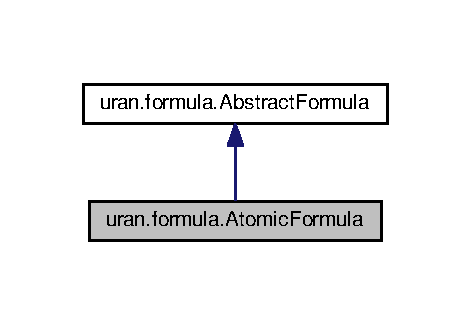
\includegraphics[width=226pt]{classuran_1_1formula_1_1_atomic_formula__inherit__graph}
\end{center}
\end{figure}


Collaboration diagram for uran.\+formula.\+Atomic\+Formula\+:
\nopagebreak
\begin{figure}[H]
\begin{center}
\leavevmode
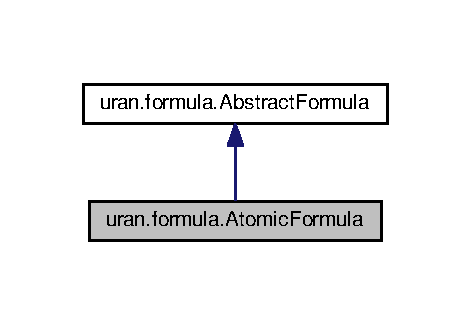
\includegraphics[width=226pt]{classuran_1_1formula_1_1_atomic_formula__coll__graph}
\end{center}
\end{figure}
\subsection*{Public Member Functions}
\begin{DoxyCompactItemize}
\item 
boolean \hyperlink{classuran_1_1formula_1_1_atomic_formula_a6884c3d5cbce1b9f4afe887fe041373b}{is\+Atomic\+Formula} ()
\end{DoxyCompactItemize}


\subsection{Detailed Description}


Definition at line 16 of file Atomic\+Formula.\+java.



\subsection{Member Function Documentation}
\hypertarget{classuran_1_1formula_1_1_atomic_formula_a6884c3d5cbce1b9f4afe887fe041373b}{}\index{uran\+::formula\+::\+Atomic\+Formula@{uran\+::formula\+::\+Atomic\+Formula}!is\+Atomic\+Formula@{is\+Atomic\+Formula}}
\index{is\+Atomic\+Formula@{is\+Atomic\+Formula}!uran\+::formula\+::\+Atomic\+Formula@{uran\+::formula\+::\+Atomic\+Formula}}
\subsubsection[{is\+Atomic\+Formula}]{\setlength{\rightskip}{0pt plus 5cm}boolean uran.\+formula.\+Atomic\+Formula.\+is\+Atomic\+Formula (
\begin{DoxyParamCaption}
{}
\end{DoxyParamCaption}
)\hspace{0.3cm}{\ttfamily [inline]}}\label{classuran_1_1formula_1_1_atomic_formula_a6884c3d5cbce1b9f4afe887fe041373b}


Definition at line 19 of file Atomic\+Formula.\+java.



The documentation for this class was generated from the following file\+:\begin{DoxyCompactItemize}
\item 
/home/haowu/uran/src/uran/formula/\hyperlink{_atomic_formula_8java}{Atomic\+Formula.\+java}\end{DoxyCompactItemize}

\hypertarget{classuran_1_1formula_1_1_binary_formula}{}\section{uran.\+formula.\+Binary\+Formula Class Reference}
\label{classuran_1_1formula_1_1_binary_formula}\index{uran.\+formula.\+Binary\+Formula@{uran.\+formula.\+Binary\+Formula}}


Inheritance diagram for uran.\+formula.\+Binary\+Formula\+:
\nopagebreak
\begin{figure}[H]
\begin{center}
\leavevmode
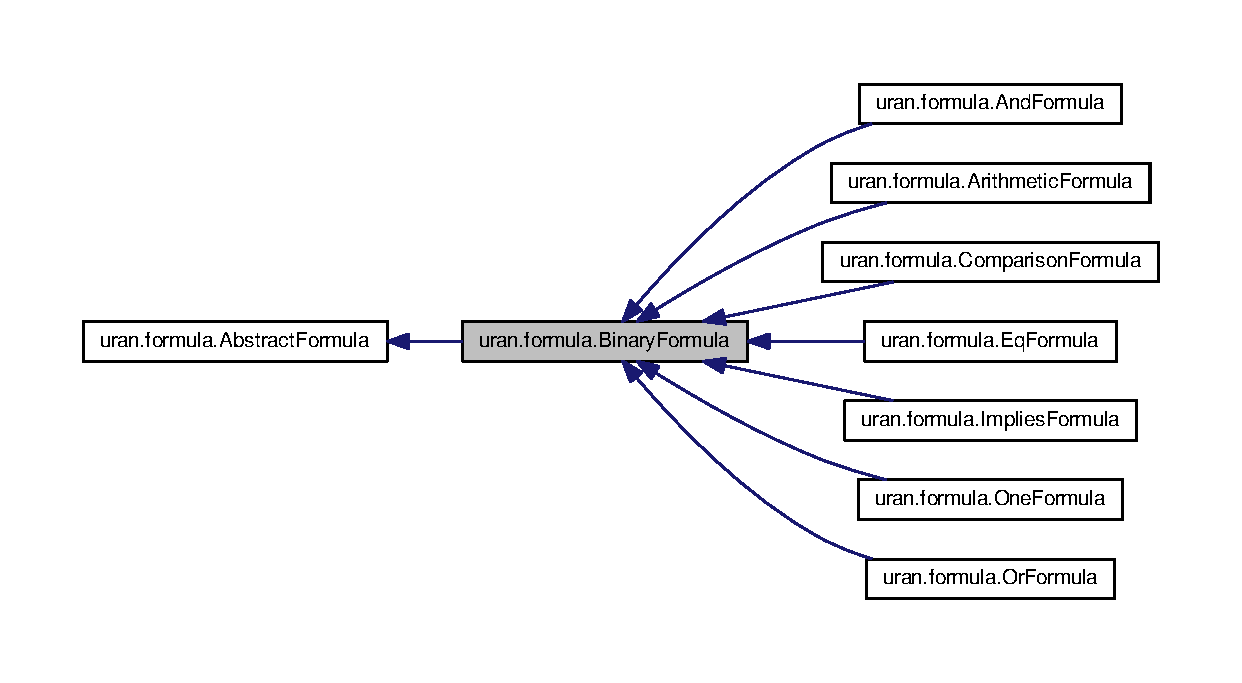
\includegraphics[width=350pt]{classuran_1_1formula_1_1_binary_formula__inherit__graph}
\end{center}
\end{figure}


Collaboration diagram for uran.\+formula.\+Binary\+Formula\+:
\nopagebreak
\begin{figure}[H]
\begin{center}
\leavevmode
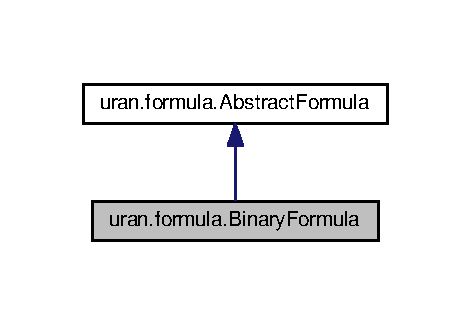
\includegraphics[width=226pt]{classuran_1_1formula_1_1_binary_formula__coll__graph}
\end{center}
\end{figure}
\subsection*{Public Member Functions}
\begin{DoxyCompactItemize}
\item 
\hyperlink{classuran_1_1formula_1_1_binary_formula_a02edc9bf8395074ae45d67417c26fc7d}{Binary\+Formula} (\hyperlink{enumuran_1_1formula_1_1_connective}{Connective} conn)
\item 
\hyperlink{classuran_1_1formula_1_1_binary_formula_a051fd65931e106b7d90aac73fff959d8}{Binary\+Formula} (\hyperlink{enumuran_1_1formula_1_1_connective}{Connective} conn, \hyperlink{classuran_1_1formula_1_1_abstract_formula}{Abstract\+Formula} \hyperlink{classuran_1_1formula_1_1_binary_formula_aca2f2d393214c782821c830525e2eba0}{left}, \hyperlink{classuran_1_1formula_1_1_abstract_formula}{Abstract\+Formula} \hyperlink{classuran_1_1formula_1_1_binary_formula_ad4643ee331c73078ccb8e7588db42469}{right})
\item 
boolean \hyperlink{classuran_1_1formula_1_1_binary_formula_ae398153453e6ae20cd6f643f189a87bb}{is\+Null} ()
\item 
\hyperlink{classuran_1_1formula_1_1_abstract_formula}{Abstract\+Formula} \hyperlink{classuran_1_1formula_1_1_binary_formula_aca2f2d393214c782821c830525e2eba0}{left} ()
\item 
\hyperlink{classuran_1_1formula_1_1_abstract_formula}{Abstract\+Formula} \hyperlink{classuran_1_1formula_1_1_binary_formula_ad4643ee331c73078ccb8e7588db42469}{right} ()
\item 
\hyperlink{enumuran_1_1formula_1_1_connective}{Connective} \hyperlink{classuran_1_1formula_1_1_binary_formula_ab1b44bdcdb9c9c287d5e073f397b7139}{connective} ()
\item 
void \hyperlink{classuran_1_1formula_1_1_binary_formula_ae6ce97787a6685a6924bc280116b5908}{set\+Left} (\hyperlink{classuran_1_1formula_1_1_abstract_formula}{Abstract\+Formula} formula)
\item 
void \hyperlink{classuran_1_1formula_1_1_binary_formula_ad68d13b744b4dfa52baca70c23a0e43e}{set\+Right} (\hyperlink{classuran_1_1formula_1_1_abstract_formula}{Abstract\+Formula} formula)
\item 
void \hyperlink{classuran_1_1formula_1_1_binary_formula_ab35c22ba91aa5a0b93a970bc59cfa265}{set\+Connective} (\hyperlink{enumuran_1_1formula_1_1_connective}{Connective} con)
\item 
String \hyperlink{classuran_1_1formula_1_1_binary_formula_a63a533db1d7231013b39aabbb13a9ed1}{to\+String} ()
\item 
abstract \hyperlink{classuran_1_1formula_1_1_binary_formula}{Binary\+Formula} \hyperlink{classuran_1_1formula_1_1_binary_formula_a304f6e9028fee95b693a0dc2d6554526}{merge} (Abstract\+Formula...\+formulas)
\item 
String \hyperlink{classuran_1_1formula_1_1_binary_formula_a6086ebd0983ed416304b5bde6bf99098}{to\+S\+M\+T2} ()
\item 
void \hyperlink{classuran_1_1formula_1_1_binary_formula_aa96ee063405718fa8e2c1c396e935a36}{accept} (\hyperlink{classuran_1_1formula_1_1visitor_1_1_abstract_visitor}{Abstract\+Visitor} visitor)
\item 
boolean \hyperlink{classuran_1_1formula_1_1_binary_formula_a7c63a1dafbe77dcb31c6ceb3eb70e208}{is\+Binary\+Formula} ()
\end{DoxyCompactItemize}


\subsection{Detailed Description}
Base class for all binary formulas \begin{DoxyAuthor}{Author}
Hao Wu 
\end{DoxyAuthor}


Definition at line 23 of file Binary\+Formula.\+java.



\subsection{Constructor \& Destructor Documentation}
\hypertarget{classuran_1_1formula_1_1_binary_formula_a02edc9bf8395074ae45d67417c26fc7d}{}\index{uran\+::formula\+::\+Binary\+Formula@{uran\+::formula\+::\+Binary\+Formula}!Binary\+Formula@{Binary\+Formula}}
\index{Binary\+Formula@{Binary\+Formula}!uran\+::formula\+::\+Binary\+Formula@{uran\+::formula\+::\+Binary\+Formula}}
\subsubsection[{Binary\+Formula}]{\setlength{\rightskip}{0pt plus 5cm}uran.\+formula.\+Binary\+Formula.\+Binary\+Formula (
\begin{DoxyParamCaption}
\item[{{\bf Connective}}]{conn}
\end{DoxyParamCaption}
)\hspace{0.3cm}{\ttfamily [inline]}}\label{classuran_1_1formula_1_1_binary_formula_a02edc9bf8395074ae45d67417c26fc7d}
setup connective 

Definition at line 31 of file Binary\+Formula.\+java.

\hypertarget{classuran_1_1formula_1_1_binary_formula_a051fd65931e106b7d90aac73fff959d8}{}\index{uran\+::formula\+::\+Binary\+Formula@{uran\+::formula\+::\+Binary\+Formula}!Binary\+Formula@{Binary\+Formula}}
\index{Binary\+Formula@{Binary\+Formula}!uran\+::formula\+::\+Binary\+Formula@{uran\+::formula\+::\+Binary\+Formula}}
\subsubsection[{Binary\+Formula}]{\setlength{\rightskip}{0pt plus 5cm}uran.\+formula.\+Binary\+Formula.\+Binary\+Formula (
\begin{DoxyParamCaption}
\item[{{\bf Connective}}]{conn, }
\item[{{\bf Abstract\+Formula}}]{left, }
\item[{{\bf Abstract\+Formula}}]{right}
\end{DoxyParamCaption}
)\hspace{0.3cm}{\ttfamily [inline]}}\label{classuran_1_1formula_1_1_binary_formula_a051fd65931e106b7d90aac73fff959d8}


Definition at line 33 of file Binary\+Formula.\+java.



\subsection{Member Function Documentation}
\hypertarget{classuran_1_1formula_1_1_binary_formula_aa96ee063405718fa8e2c1c396e935a36}{}\index{uran\+::formula\+::\+Binary\+Formula@{uran\+::formula\+::\+Binary\+Formula}!accept@{accept}}
\index{accept@{accept}!uran\+::formula\+::\+Binary\+Formula@{uran\+::formula\+::\+Binary\+Formula}}
\subsubsection[{accept}]{\setlength{\rightskip}{0pt plus 5cm}void uran.\+formula.\+Binary\+Formula.\+accept (
\begin{DoxyParamCaption}
\item[{{\bf Abstract\+Visitor}}]{visitor}
\end{DoxyParamCaption}
)\hspace{0.3cm}{\ttfamily [inline]}}\label{classuran_1_1formula_1_1_binary_formula_aa96ee063405718fa8e2c1c396e935a36}


Definition at line 102 of file Binary\+Formula.\+java.

\hypertarget{classuran_1_1formula_1_1_binary_formula_ab1b44bdcdb9c9c287d5e073f397b7139}{}\index{uran\+::formula\+::\+Binary\+Formula@{uran\+::formula\+::\+Binary\+Formula}!connective@{connective}}
\index{connective@{connective}!uran\+::formula\+::\+Binary\+Formula@{uran\+::formula\+::\+Binary\+Formula}}
\subsubsection[{connective}]{\setlength{\rightskip}{0pt plus 5cm}{\bf Connective} uran.\+formula.\+Binary\+Formula.\+connective (
\begin{DoxyParamCaption}
{}
\end{DoxyParamCaption}
)\hspace{0.3cm}{\ttfamily [inline]}}\label{classuran_1_1formula_1_1_binary_formula_ab1b44bdcdb9c9c287d5e073f397b7139}
\begin{DoxyReturn}{Returns}
the connective 
\end{DoxyReturn}


Definition at line 62 of file Binary\+Formula.\+java.

\hypertarget{classuran_1_1formula_1_1_binary_formula_a7c63a1dafbe77dcb31c6ceb3eb70e208}{}\index{uran\+::formula\+::\+Binary\+Formula@{uran\+::formula\+::\+Binary\+Formula}!is\+Binary\+Formula@{is\+Binary\+Formula}}
\index{is\+Binary\+Formula@{is\+Binary\+Formula}!uran\+::formula\+::\+Binary\+Formula@{uran\+::formula\+::\+Binary\+Formula}}
\subsubsection[{is\+Binary\+Formula}]{\setlength{\rightskip}{0pt plus 5cm}boolean uran.\+formula.\+Binary\+Formula.\+is\+Binary\+Formula (
\begin{DoxyParamCaption}
{}
\end{DoxyParamCaption}
)\hspace{0.3cm}{\ttfamily [inline]}}\label{classuran_1_1formula_1_1_binary_formula_a7c63a1dafbe77dcb31c6ceb3eb70e208}


Definition at line 107 of file Binary\+Formula.\+java.

\hypertarget{classuran_1_1formula_1_1_binary_formula_ae398153453e6ae20cd6f643f189a87bb}{}\index{uran\+::formula\+::\+Binary\+Formula@{uran\+::formula\+::\+Binary\+Formula}!is\+Null@{is\+Null}}
\index{is\+Null@{is\+Null}!uran\+::formula\+::\+Binary\+Formula@{uran\+::formula\+::\+Binary\+Formula}}
\subsubsection[{is\+Null}]{\setlength{\rightskip}{0pt plus 5cm}boolean uran.\+formula.\+Binary\+Formula.\+is\+Null (
\begin{DoxyParamCaption}
{}
\end{DoxyParamCaption}
)\hspace{0.3cm}{\ttfamily [inline]}}\label{classuran_1_1formula_1_1_binary_formula_ae398153453e6ae20cd6f643f189a87bb}
if both left and right nodes are null, then this formula is considered to be null. 

Definition at line 43 of file Binary\+Formula.\+java.

\hypertarget{classuran_1_1formula_1_1_binary_formula_aca2f2d393214c782821c830525e2eba0}{}\index{uran\+::formula\+::\+Binary\+Formula@{uran\+::formula\+::\+Binary\+Formula}!left@{left}}
\index{left@{left}!uran\+::formula\+::\+Binary\+Formula@{uran\+::formula\+::\+Binary\+Formula}}
\subsubsection[{left}]{\setlength{\rightskip}{0pt plus 5cm}{\bf Abstract\+Formula} uran.\+formula.\+Binary\+Formula.\+left (
\begin{DoxyParamCaption}
{}
\end{DoxyParamCaption}
)\hspace{0.3cm}{\ttfamily [inline]}}\label{classuran_1_1formula_1_1_binary_formula_aca2f2d393214c782821c830525e2eba0}
\begin{DoxyReturn}{Returns}
the left node 
\end{DoxyReturn}


Definition at line 49 of file Binary\+Formula.\+java.

\hypertarget{classuran_1_1formula_1_1_binary_formula_a304f6e9028fee95b693a0dc2d6554526}{}\index{uran\+::formula\+::\+Binary\+Formula@{uran\+::formula\+::\+Binary\+Formula}!merge@{merge}}
\index{merge@{merge}!uran\+::formula\+::\+Binary\+Formula@{uran\+::formula\+::\+Binary\+Formula}}
\subsubsection[{merge}]{\setlength{\rightskip}{0pt plus 5cm}abstract {\bf Binary\+Formula} uran.\+formula.\+Binary\+Formula.\+merge (
\begin{DoxyParamCaption}
\item[{Abstract\+Formula...}]{formulas}
\end{DoxyParamCaption}
)\hspace{0.3cm}{\ttfamily [abstract]}}\label{classuran_1_1formula_1_1_binary_formula_a304f6e9028fee95b693a0dc2d6554526}
merge a series of binary formulas. 
\begin{DoxyParams}{Parameters}
{\em formulas} & formulas to be merged \\
\hline
\end{DoxyParams}
\hypertarget{classuran_1_1formula_1_1_binary_formula_ad4643ee331c73078ccb8e7588db42469}{}\index{uran\+::formula\+::\+Binary\+Formula@{uran\+::formula\+::\+Binary\+Formula}!right@{right}}
\index{right@{right}!uran\+::formula\+::\+Binary\+Formula@{uran\+::formula\+::\+Binary\+Formula}}
\subsubsection[{right}]{\setlength{\rightskip}{0pt plus 5cm}{\bf Abstract\+Formula} uran.\+formula.\+Binary\+Formula.\+right (
\begin{DoxyParamCaption}
{}
\end{DoxyParamCaption}
)\hspace{0.3cm}{\ttfamily [inline]}}\label{classuran_1_1formula_1_1_binary_formula_ad4643ee331c73078ccb8e7588db42469}
\begin{DoxyReturn}{Returns}
the right node 
\end{DoxyReturn}


Definition at line 56 of file Binary\+Formula.\+java.

\hypertarget{classuran_1_1formula_1_1_binary_formula_ab35c22ba91aa5a0b93a970bc59cfa265}{}\index{uran\+::formula\+::\+Binary\+Formula@{uran\+::formula\+::\+Binary\+Formula}!set\+Connective@{set\+Connective}}
\index{set\+Connective@{set\+Connective}!uran\+::formula\+::\+Binary\+Formula@{uran\+::formula\+::\+Binary\+Formula}}
\subsubsection[{set\+Connective}]{\setlength{\rightskip}{0pt plus 5cm}void uran.\+formula.\+Binary\+Formula.\+set\+Connective (
\begin{DoxyParamCaption}
\item[{{\bf Connective}}]{con}
\end{DoxyParamCaption}
)\hspace{0.3cm}{\ttfamily [inline]}}\label{classuran_1_1formula_1_1_binary_formula_ab35c22ba91aa5a0b93a970bc59cfa265}


Definition at line 84 of file Binary\+Formula.\+java.

\hypertarget{classuran_1_1formula_1_1_binary_formula_ae6ce97787a6685a6924bc280116b5908}{}\index{uran\+::formula\+::\+Binary\+Formula@{uran\+::formula\+::\+Binary\+Formula}!set\+Left@{set\+Left}}
\index{set\+Left@{set\+Left}!uran\+::formula\+::\+Binary\+Formula@{uran\+::formula\+::\+Binary\+Formula}}
\subsubsection[{set\+Left}]{\setlength{\rightskip}{0pt plus 5cm}void uran.\+formula.\+Binary\+Formula.\+set\+Left (
\begin{DoxyParamCaption}
\item[{{\bf Abstract\+Formula}}]{formula}
\end{DoxyParamCaption}
)\hspace{0.3cm}{\ttfamily [inline]}}\label{classuran_1_1formula_1_1_binary_formula_ae6ce97787a6685a6924bc280116b5908}
set up a new left node. 
\begin{DoxyParams}{Parameters}
{\em formula} & the new left node \\
\hline
\end{DoxyParams}


Definition at line 70 of file Binary\+Formula.\+java.

\hypertarget{classuran_1_1formula_1_1_binary_formula_ad68d13b744b4dfa52baca70c23a0e43e}{}\index{uran\+::formula\+::\+Binary\+Formula@{uran\+::formula\+::\+Binary\+Formula}!set\+Right@{set\+Right}}
\index{set\+Right@{set\+Right}!uran\+::formula\+::\+Binary\+Formula@{uran\+::formula\+::\+Binary\+Formula}}
\subsubsection[{set\+Right}]{\setlength{\rightskip}{0pt plus 5cm}void uran.\+formula.\+Binary\+Formula.\+set\+Right (
\begin{DoxyParamCaption}
\item[{{\bf Abstract\+Formula}}]{formula}
\end{DoxyParamCaption}
)\hspace{0.3cm}{\ttfamily [inline]}}\label{classuran_1_1formula_1_1_binary_formula_ad68d13b744b4dfa52baca70c23a0e43e}
set up a new right node. 
\begin{DoxyParams}{Parameters}
{\em formula} & the new right node \\
\hline
\end{DoxyParams}


Definition at line 79 of file Binary\+Formula.\+java.

\hypertarget{classuran_1_1formula_1_1_binary_formula_a6086ebd0983ed416304b5bde6bf99098}{}\index{uran\+::formula\+::\+Binary\+Formula@{uran\+::formula\+::\+Binary\+Formula}!to\+S\+M\+T2@{to\+S\+M\+T2}}
\index{to\+S\+M\+T2@{to\+S\+M\+T2}!uran\+::formula\+::\+Binary\+Formula@{uran\+::formula\+::\+Binary\+Formula}}
\subsubsection[{to\+S\+M\+T2}]{\setlength{\rightskip}{0pt plus 5cm}String uran.\+formula.\+Binary\+Formula.\+to\+S\+M\+T2 (
\begin{DoxyParamCaption}
{}
\end{DoxyParamCaption}
)\hspace{0.3cm}{\ttfamily [inline]}}\label{classuran_1_1formula_1_1_binary_formula_a6086ebd0983ed416304b5bde6bf99098}


Definition at line 97 of file Binary\+Formula.\+java.

\hypertarget{classuran_1_1formula_1_1_binary_formula_a63a533db1d7231013b39aabbb13a9ed1}{}\index{uran\+::formula\+::\+Binary\+Formula@{uran\+::formula\+::\+Binary\+Formula}!to\+String@{to\+String}}
\index{to\+String@{to\+String}!uran\+::formula\+::\+Binary\+Formula@{uran\+::formula\+::\+Binary\+Formula}}
\subsubsection[{to\+String}]{\setlength{\rightskip}{0pt plus 5cm}String uran.\+formula.\+Binary\+Formula.\+to\+String (
\begin{DoxyParamCaption}
{}
\end{DoxyParamCaption}
)\hspace{0.3cm}{\ttfamily [inline]}}\label{classuran_1_1formula_1_1_binary_formula_a63a533db1d7231013b39aabbb13a9ed1}


Definition at line 86 of file Binary\+Formula.\+java.



The documentation for this class was generated from the following file\+:\begin{DoxyCompactItemize}
\item 
/home/haowu/uran/src/uran/formula/\hyperlink{_binary_formula_8java}{Binary\+Formula.\+java}\end{DoxyCompactItemize}

\hypertarget{classuran_1_1formula_1_1cnf_1_1_binary_gate}{}\section{uran.\+formula.\+cnf.\+Binary\+Gate Class Reference}
\label{classuran_1_1formula_1_1cnf_1_1_binary_gate}\index{uran.\+formula.\+cnf.\+Binary\+Gate@{uran.\+formula.\+cnf.\+Binary\+Gate}}


Inheritance diagram for uran.\+formula.\+cnf.\+Binary\+Gate\+:
\nopagebreak
\begin{figure}[H]
\begin{center}
\leavevmode
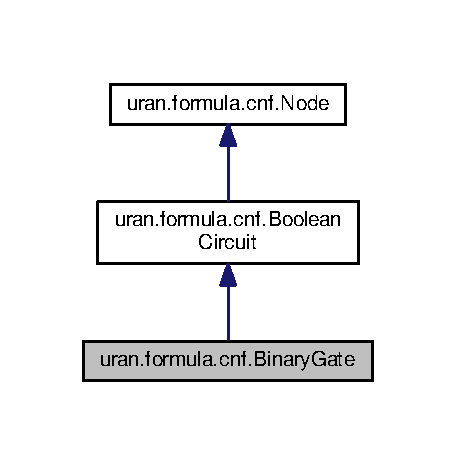
\includegraphics[width=219pt]{classuran_1_1formula_1_1cnf_1_1_binary_gate__inherit__graph}
\end{center}
\end{figure}


Collaboration diagram for uran.\+formula.\+cnf.\+Binary\+Gate\+:
\nopagebreak
\begin{figure}[H]
\begin{center}
\leavevmode
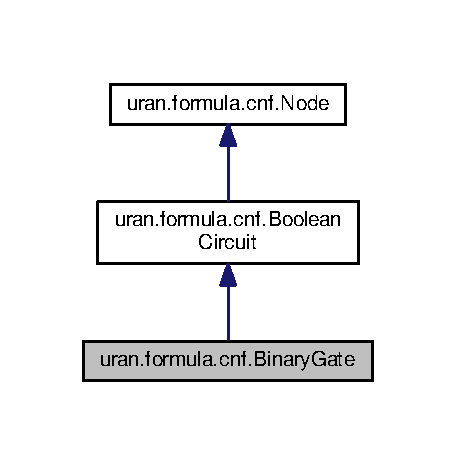
\includegraphics[width=219pt]{classuran_1_1formula_1_1cnf_1_1_binary_gate__coll__graph}
\end{center}
\end{figure}
\subsection*{Public Member Functions}
\begin{DoxyCompactItemize}
\item 
\hyperlink{classuran_1_1formula_1_1cnf_1_1_binary_gate_a5328f117f419aed43f46810c6eb64800}{Binary\+Gate} (int n, \hyperlink{classuran_1_1formula_1_1cnf_1_1_boolean_circuit}{Boolean\+Circuit} c1, \hyperlink{classuran_1_1formula_1_1cnf_1_1_boolean_circuit}{Boolean\+Circuit} c2)
\item 
String \hyperlink{classuran_1_1formula_1_1cnf_1_1_binary_gate_a80351a9a44c1169bf5fb33bbb37402f5}{to\+String} ()
\item 
\hyperlink{classuran_1_1formula_1_1cnf_1_1_boolean_circuit}{Boolean\+Circuit} \hyperlink{classuran_1_1formula_1_1cnf_1_1_binary_gate_abd94a491dcf0817140225d38234c6cf8}{input0} ()
\item 
\hyperlink{classuran_1_1formula_1_1cnf_1_1_boolean_circuit}{Boolean\+Circuit} \hyperlink{classuran_1_1formula_1_1cnf_1_1_binary_gate_a85ac51e7db1b845ce851ac87fc972353}{input1} ()
\item 
boolean \hyperlink{classuran_1_1formula_1_1cnf_1_1_binary_gate_a4136bcf8f1cc242690331bfa428442fd}{is\+Binary\+Gate} ()
\item 
int \hyperlink{classuran_1_1formula_1_1cnf_1_1_binary_gate_adfd7457fdeba97281ec208de217382e9}{operator} ()
\item 
void \hyperlink{classuran_1_1formula_1_1cnf_1_1_binary_gate_a62e1df3f6df1ae5846de86fe23d42491}{accept} (\hyperlink{classuran_1_1formula_1_1cnf_1_1visitor_1_1_abstract_visitor}{Abstract\+Visitor} v)
\end{DoxyCompactItemize}
\subsection*{Additional Inherited Members}


\subsection{Detailed Description}


Definition at line 18 of file Binary\+Gate.\+java.



\subsection{Constructor \& Destructor Documentation}
\hypertarget{classuran_1_1formula_1_1cnf_1_1_binary_gate_a5328f117f419aed43f46810c6eb64800}{}\index{uran\+::formula\+::cnf\+::\+Binary\+Gate@{uran\+::formula\+::cnf\+::\+Binary\+Gate}!Binary\+Gate@{Binary\+Gate}}
\index{Binary\+Gate@{Binary\+Gate}!uran\+::formula\+::cnf\+::\+Binary\+Gate@{uran\+::formula\+::cnf\+::\+Binary\+Gate}}
\subsubsection[{Binary\+Gate}]{\setlength{\rightskip}{0pt plus 5cm}uran.\+formula.\+cnf.\+Binary\+Gate.\+Binary\+Gate (
\begin{DoxyParamCaption}
\item[{int}]{n, }
\item[{{\bf Boolean\+Circuit}}]{c1, }
\item[{{\bf Boolean\+Circuit}}]{c2}
\end{DoxyParamCaption}
)\hspace{0.3cm}{\ttfamily [inline]}}\label{classuran_1_1formula_1_1cnf_1_1_binary_gate_a5328f117f419aed43f46810c6eb64800}


Definition at line 23 of file Binary\+Gate.\+java.



\subsection{Member Function Documentation}
\hypertarget{classuran_1_1formula_1_1cnf_1_1_binary_gate_a62e1df3f6df1ae5846de86fe23d42491}{}\index{uran\+::formula\+::cnf\+::\+Binary\+Gate@{uran\+::formula\+::cnf\+::\+Binary\+Gate}!accept@{accept}}
\index{accept@{accept}!uran\+::formula\+::cnf\+::\+Binary\+Gate@{uran\+::formula\+::cnf\+::\+Binary\+Gate}}
\subsubsection[{accept}]{\setlength{\rightskip}{0pt plus 5cm}void uran.\+formula.\+cnf.\+Binary\+Gate.\+accept (
\begin{DoxyParamCaption}
\item[{{\bf Abstract\+Visitor}}]{v}
\end{DoxyParamCaption}
)\hspace{0.3cm}{\ttfamily [inline]}}\label{classuran_1_1formula_1_1cnf_1_1_binary_gate_a62e1df3f6df1ae5846de86fe23d42491}


Definition at line 39 of file Binary\+Gate.\+java.

\hypertarget{classuran_1_1formula_1_1cnf_1_1_binary_gate_abd94a491dcf0817140225d38234c6cf8}{}\index{uran\+::formula\+::cnf\+::\+Binary\+Gate@{uran\+::formula\+::cnf\+::\+Binary\+Gate}!input0@{input0}}
\index{input0@{input0}!uran\+::formula\+::cnf\+::\+Binary\+Gate@{uran\+::formula\+::cnf\+::\+Binary\+Gate}}
\subsubsection[{input0}]{\setlength{\rightskip}{0pt plus 5cm}{\bf Boolean\+Circuit} uran.\+formula.\+cnf.\+Binary\+Gate.\+input0 (
\begin{DoxyParamCaption}
{}
\end{DoxyParamCaption}
)\hspace{0.3cm}{\ttfamily [inline]}}\label{classuran_1_1formula_1_1cnf_1_1_binary_gate_abd94a491dcf0817140225d38234c6cf8}


Definition at line 34 of file Binary\+Gate.\+java.

\hypertarget{classuran_1_1formula_1_1cnf_1_1_binary_gate_a85ac51e7db1b845ce851ac87fc972353}{}\index{uran\+::formula\+::cnf\+::\+Binary\+Gate@{uran\+::formula\+::cnf\+::\+Binary\+Gate}!input1@{input1}}
\index{input1@{input1}!uran\+::formula\+::cnf\+::\+Binary\+Gate@{uran\+::formula\+::cnf\+::\+Binary\+Gate}}
\subsubsection[{input1}]{\setlength{\rightskip}{0pt plus 5cm}{\bf Boolean\+Circuit} uran.\+formula.\+cnf.\+Binary\+Gate.\+input1 (
\begin{DoxyParamCaption}
{}
\end{DoxyParamCaption}
)\hspace{0.3cm}{\ttfamily [inline]}}\label{classuran_1_1formula_1_1cnf_1_1_binary_gate_a85ac51e7db1b845ce851ac87fc972353}


Definition at line 35 of file Binary\+Gate.\+java.

\hypertarget{classuran_1_1formula_1_1cnf_1_1_binary_gate_a4136bcf8f1cc242690331bfa428442fd}{}\index{uran\+::formula\+::cnf\+::\+Binary\+Gate@{uran\+::formula\+::cnf\+::\+Binary\+Gate}!is\+Binary\+Gate@{is\+Binary\+Gate}}
\index{is\+Binary\+Gate@{is\+Binary\+Gate}!uran\+::formula\+::cnf\+::\+Binary\+Gate@{uran\+::formula\+::cnf\+::\+Binary\+Gate}}
\subsubsection[{is\+Binary\+Gate}]{\setlength{\rightskip}{0pt plus 5cm}boolean uran.\+formula.\+cnf.\+Binary\+Gate.\+is\+Binary\+Gate (
\begin{DoxyParamCaption}
{}
\end{DoxyParamCaption}
)\hspace{0.3cm}{\ttfamily [inline]}}\label{classuran_1_1formula_1_1cnf_1_1_binary_gate_a4136bcf8f1cc242690331bfa428442fd}


Definition at line 36 of file Binary\+Gate.\+java.

\hypertarget{classuran_1_1formula_1_1cnf_1_1_binary_gate_adfd7457fdeba97281ec208de217382e9}{}\index{uran\+::formula\+::cnf\+::\+Binary\+Gate@{uran\+::formula\+::cnf\+::\+Binary\+Gate}!operator@{operator}}
\index{operator@{operator}!uran\+::formula\+::cnf\+::\+Binary\+Gate@{uran\+::formula\+::cnf\+::\+Binary\+Gate}}
\subsubsection[{operator}]{\setlength{\rightskip}{0pt plus 5cm}int uran.\+formula.\+cnf.\+Binary\+Gate.\+operator (
\begin{DoxyParamCaption}
{}
\end{DoxyParamCaption}
)\hspace{0.3cm}{\ttfamily [inline]}}\label{classuran_1_1formula_1_1cnf_1_1_binary_gate_adfd7457fdeba97281ec208de217382e9}


Definition at line 38 of file Binary\+Gate.\+java.

\hypertarget{classuran_1_1formula_1_1cnf_1_1_binary_gate_a80351a9a44c1169bf5fb33bbb37402f5}{}\index{uran\+::formula\+::cnf\+::\+Binary\+Gate@{uran\+::formula\+::cnf\+::\+Binary\+Gate}!to\+String@{to\+String}}
\index{to\+String@{to\+String}!uran\+::formula\+::cnf\+::\+Binary\+Gate@{uran\+::formula\+::cnf\+::\+Binary\+Gate}}
\subsubsection[{to\+String}]{\setlength{\rightskip}{0pt plus 5cm}String uran.\+formula.\+cnf.\+Binary\+Gate.\+to\+String (
\begin{DoxyParamCaption}
{}
\end{DoxyParamCaption}
)\hspace{0.3cm}{\ttfamily [inline]}}\label{classuran_1_1formula_1_1cnf_1_1_binary_gate_a80351a9a44c1169bf5fb33bbb37402f5}


Definition at line 30 of file Binary\+Gate.\+java.



The documentation for this class was generated from the following file\+:\begin{DoxyCompactItemize}
\item 
/home/haowu/uran/src/uran/formula/cnf/\hyperlink{_binary_gate_8java}{Binary\+Gate.\+java}\end{DoxyCompactItemize}

\hypertarget{classuran_1_1formula_1_1type_1_1_bool}{}\section{uran.\+formula.\+type.\+Bool Class Reference}
\label{classuran_1_1formula_1_1type_1_1_bool}\index{uran.\+formula.\+type.\+Bool@{uran.\+formula.\+type.\+Bool}}


Inheritance diagram for uran.\+formula.\+type.\+Bool\+:
\nopagebreak
\begin{figure}[H]
\begin{center}
\leavevmode
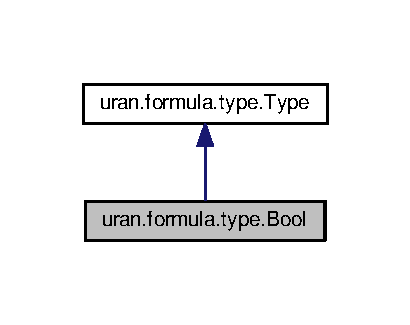
\includegraphics[width=197pt]{classuran_1_1formula_1_1type_1_1_bool__inherit__graph}
\end{center}
\end{figure}


Collaboration diagram for uran.\+formula.\+type.\+Bool\+:
\nopagebreak
\begin{figure}[H]
\begin{center}
\leavevmode
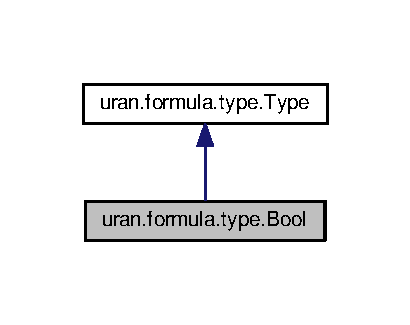
\includegraphics[width=197pt]{classuran_1_1formula_1_1type_1_1_bool__coll__graph}
\end{center}
\end{figure}
\subsection*{Public Member Functions}
\begin{DoxyCompactItemize}
\item 
\hyperlink{classuran_1_1formula_1_1type_1_1_bool_aa476c4ed0e0023859f4fe28279ac97a1}{Bool} ()
\item 
String \hyperlink{classuran_1_1formula_1_1type_1_1_bool_a7b9d46f551b2a9e84c63476f9805c852}{name} ()
\item 
boolean \hyperlink{classuran_1_1formula_1_1type_1_1_bool_aafddfb259fe050ea4499ae0704c30bed}{is\+Bool} ()
\item 
String \hyperlink{classuran_1_1formula_1_1type_1_1_bool_ab20f47a4bd2f38f47c1d4b4bda13c58f}{to\+String} ()
\end{DoxyCompactItemize}
\subsection*{Additional Inherited Members}


\subsection{Detailed Description}


Definition at line 16 of file Bool.\+java.



\subsection{Constructor \& Destructor Documentation}
\hypertarget{classuran_1_1formula_1_1type_1_1_bool_aa476c4ed0e0023859f4fe28279ac97a1}{}\index{uran\+::formula\+::type\+::\+Bool@{uran\+::formula\+::type\+::\+Bool}!Bool@{Bool}}
\index{Bool@{Bool}!uran\+::formula\+::type\+::\+Bool@{uran\+::formula\+::type\+::\+Bool}}
\subsubsection[{Bool}]{\setlength{\rightskip}{0pt plus 5cm}uran.\+formula.\+type.\+Bool.\+Bool (
\begin{DoxyParamCaption}
{}
\end{DoxyParamCaption}
)\hspace{0.3cm}{\ttfamily [inline]}}\label{classuran_1_1formula_1_1type_1_1_bool_aa476c4ed0e0023859f4fe28279ac97a1}


Definition at line 18 of file Bool.\+java.



\subsection{Member Function Documentation}
\hypertarget{classuran_1_1formula_1_1type_1_1_bool_aafddfb259fe050ea4499ae0704c30bed}{}\index{uran\+::formula\+::type\+::\+Bool@{uran\+::formula\+::type\+::\+Bool}!is\+Bool@{is\+Bool}}
\index{is\+Bool@{is\+Bool}!uran\+::formula\+::type\+::\+Bool@{uran\+::formula\+::type\+::\+Bool}}
\subsubsection[{is\+Bool}]{\setlength{\rightskip}{0pt plus 5cm}boolean uran.\+formula.\+type.\+Bool.\+is\+Bool (
\begin{DoxyParamCaption}
{}
\end{DoxyParamCaption}
)\hspace{0.3cm}{\ttfamily [inline]}}\label{classuran_1_1formula_1_1type_1_1_bool_aafddfb259fe050ea4499ae0704c30bed}


Definition at line 28 of file Bool.\+java.

\hypertarget{classuran_1_1formula_1_1type_1_1_bool_a7b9d46f551b2a9e84c63476f9805c852}{}\index{uran\+::formula\+::type\+::\+Bool@{uran\+::formula\+::type\+::\+Bool}!name@{name}}
\index{name@{name}!uran\+::formula\+::type\+::\+Bool@{uran\+::formula\+::type\+::\+Bool}}
\subsubsection[{name}]{\setlength{\rightskip}{0pt plus 5cm}String uran.\+formula.\+type.\+Bool.\+name (
\begin{DoxyParamCaption}
{}
\end{DoxyParamCaption}
)\hspace{0.3cm}{\ttfamily [inline]}}\label{classuran_1_1formula_1_1type_1_1_bool_a7b9d46f551b2a9e84c63476f9805c852}


Definition at line 23 of file Bool.\+java.

\hypertarget{classuran_1_1formula_1_1type_1_1_bool_ab20f47a4bd2f38f47c1d4b4bda13c58f}{}\index{uran\+::formula\+::type\+::\+Bool@{uran\+::formula\+::type\+::\+Bool}!to\+String@{to\+String}}
\index{to\+String@{to\+String}!uran\+::formula\+::type\+::\+Bool@{uran\+::formula\+::type\+::\+Bool}}
\subsubsection[{to\+String}]{\setlength{\rightskip}{0pt plus 5cm}String uran.\+formula.\+type.\+Bool.\+to\+String (
\begin{DoxyParamCaption}
{}
\end{DoxyParamCaption}
)\hspace{0.3cm}{\ttfamily [inline]}}\label{classuran_1_1formula_1_1type_1_1_bool_ab20f47a4bd2f38f47c1d4b4bda13c58f}


Definition at line 30 of file Bool.\+java.



The documentation for this class was generated from the following file\+:\begin{DoxyCompactItemize}
\item 
/home/haowu/uran/src/uran/formula/type/\hyperlink{_bool_8java}{Bool.\+java}\end{DoxyCompactItemize}

\hypertarget{classuran_1_1formula_1_1cnf_1_1_boolean_circuit}{}\section{uran.\+formula.\+cnf.\+Boolean\+Circuit Class Reference}
\label{classuran_1_1formula_1_1cnf_1_1_boolean_circuit}\index{uran.\+formula.\+cnf.\+Boolean\+Circuit@{uran.\+formula.\+cnf.\+Boolean\+Circuit}}


Inheritance diagram for uran.\+formula.\+cnf.\+Boolean\+Circuit\+:
\nopagebreak
\begin{figure}[H]
\begin{center}
\leavevmode
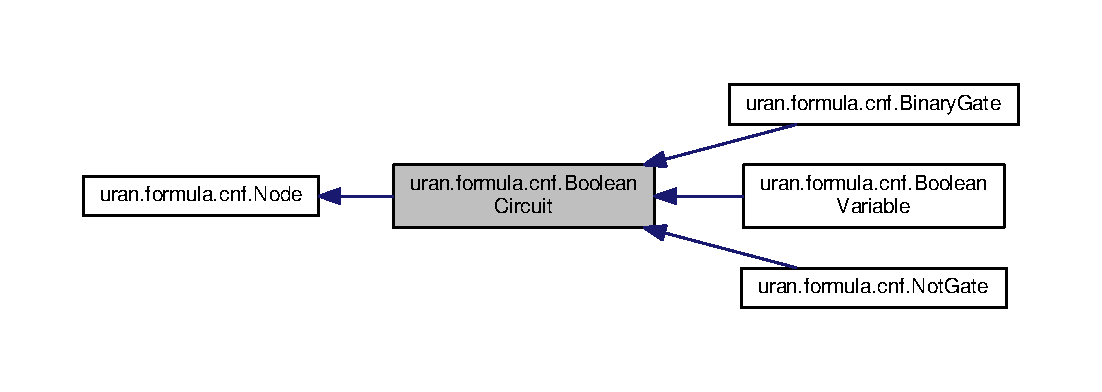
\includegraphics[width=350pt]{classuran_1_1formula_1_1cnf_1_1_boolean_circuit__inherit__graph}
\end{center}
\end{figure}


Collaboration diagram for uran.\+formula.\+cnf.\+Boolean\+Circuit\+:
\nopagebreak
\begin{figure}[H]
\begin{center}
\leavevmode
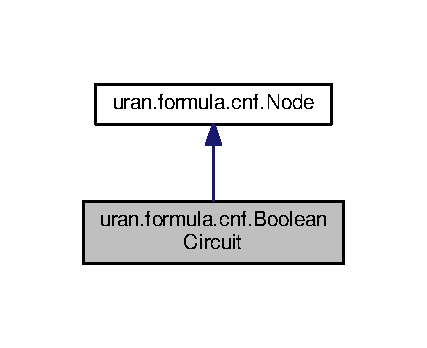
\includegraphics[width=205pt]{classuran_1_1formula_1_1cnf_1_1_boolean_circuit__coll__graph}
\end{center}
\end{figure}
\subsection*{Public Member Functions}
\begin{DoxyCompactItemize}
\item 
long \hyperlink{classuran_1_1formula_1_1cnf_1_1_boolean_circuit_ae555af28a0fe4854b044ac7c03f2900a}{label} ()
\item 
void \hyperlink{classuran_1_1formula_1_1cnf_1_1_boolean_circuit_ab54aa4d58efb76b3036ecc7c364c3965}{assign} (long k)
\item 
long \hyperlink{classuran_1_1formula_1_1cnf_1_1_boolean_circuit_ac32a42c7cf395447b5d093c40f5ddb60}{negation} ()
\item 
boolean \hyperlink{classuran_1_1formula_1_1cnf_1_1_boolean_circuit_a391d1368a9278df4a09852df1c696c59}{is\+Boolean\+Variable} ()
\item 
boolean \hyperlink{classuran_1_1formula_1_1cnf_1_1_boolean_circuit_ae935b68b31baa8998267dbd9d3e8b790}{is\+Binary\+Gate} ()
\item 
boolean \hyperlink{classuran_1_1formula_1_1cnf_1_1_boolean_circuit_a57d155d7d00066d0fcc057c9f57ec669}{is\+Not\+Gate} ()
\item 
abstract void \hyperlink{classuran_1_1formula_1_1cnf_1_1_boolean_circuit_aef2638857ae58fb05b6db1eb2be25565}{accept} (\hyperlink{classuran_1_1formula_1_1cnf_1_1visitor_1_1_abstract_visitor}{Abstract\+Visitor} v)
\end{DoxyCompactItemize}
\subsection*{Static Public Attributes}
\begin{DoxyCompactItemize}
\item 
static final int \hyperlink{classuran_1_1formula_1_1cnf_1_1_boolean_circuit_a390c29de655dcf8134ad839d29d6192c}{U\+N\+D\+E\+F\+I\+N\+E\+D} =-\/1
\end{DoxyCompactItemize}


\subsection{Detailed Description}


Definition at line 19 of file Boolean\+Circuit.\+java.



\subsection{Member Function Documentation}
\hypertarget{classuran_1_1formula_1_1cnf_1_1_boolean_circuit_aef2638857ae58fb05b6db1eb2be25565}{}\index{uran\+::formula\+::cnf\+::\+Boolean\+Circuit@{uran\+::formula\+::cnf\+::\+Boolean\+Circuit}!accept@{accept}}
\index{accept@{accept}!uran\+::formula\+::cnf\+::\+Boolean\+Circuit@{uran\+::formula\+::cnf\+::\+Boolean\+Circuit}}
\subsubsection[{accept}]{\setlength{\rightskip}{0pt plus 5cm}abstract void uran.\+formula.\+cnf.\+Boolean\+Circuit.\+accept (
\begin{DoxyParamCaption}
\item[{{\bf Abstract\+Visitor}}]{v}
\end{DoxyParamCaption}
)\hspace{0.3cm}{\ttfamily [abstract]}}\label{classuran_1_1formula_1_1cnf_1_1_boolean_circuit_aef2638857ae58fb05b6db1eb2be25565}
\hypertarget{classuran_1_1formula_1_1cnf_1_1_boolean_circuit_ab54aa4d58efb76b3036ecc7c364c3965}{}\index{uran\+::formula\+::cnf\+::\+Boolean\+Circuit@{uran\+::formula\+::cnf\+::\+Boolean\+Circuit}!assign@{assign}}
\index{assign@{assign}!uran\+::formula\+::cnf\+::\+Boolean\+Circuit@{uran\+::formula\+::cnf\+::\+Boolean\+Circuit}}
\subsubsection[{assign}]{\setlength{\rightskip}{0pt plus 5cm}void uran.\+formula.\+cnf.\+Boolean\+Circuit.\+assign (
\begin{DoxyParamCaption}
\item[{long}]{k}
\end{DoxyParamCaption}
)\hspace{0.3cm}{\ttfamily [inline]}}\label{classuran_1_1formula_1_1cnf_1_1_boolean_circuit_ab54aa4d58efb76b3036ecc7c364c3965}


Definition at line 24 of file Boolean\+Circuit.\+java.

\hypertarget{classuran_1_1formula_1_1cnf_1_1_boolean_circuit_ae935b68b31baa8998267dbd9d3e8b790}{}\index{uran\+::formula\+::cnf\+::\+Boolean\+Circuit@{uran\+::formula\+::cnf\+::\+Boolean\+Circuit}!is\+Binary\+Gate@{is\+Binary\+Gate}}
\index{is\+Binary\+Gate@{is\+Binary\+Gate}!uran\+::formula\+::cnf\+::\+Boolean\+Circuit@{uran\+::formula\+::cnf\+::\+Boolean\+Circuit}}
\subsubsection[{is\+Binary\+Gate}]{\setlength{\rightskip}{0pt plus 5cm}boolean uran.\+formula.\+cnf.\+Boolean\+Circuit.\+is\+Binary\+Gate (
\begin{DoxyParamCaption}
{}
\end{DoxyParamCaption}
)\hspace{0.3cm}{\ttfamily [inline]}}\label{classuran_1_1formula_1_1cnf_1_1_boolean_circuit_ae935b68b31baa8998267dbd9d3e8b790}


Definition at line 31 of file Boolean\+Circuit.\+java.

\hypertarget{classuran_1_1formula_1_1cnf_1_1_boolean_circuit_a391d1368a9278df4a09852df1c696c59}{}\index{uran\+::formula\+::cnf\+::\+Boolean\+Circuit@{uran\+::formula\+::cnf\+::\+Boolean\+Circuit}!is\+Boolean\+Variable@{is\+Boolean\+Variable}}
\index{is\+Boolean\+Variable@{is\+Boolean\+Variable}!uran\+::formula\+::cnf\+::\+Boolean\+Circuit@{uran\+::formula\+::cnf\+::\+Boolean\+Circuit}}
\subsubsection[{is\+Boolean\+Variable}]{\setlength{\rightskip}{0pt plus 5cm}boolean uran.\+formula.\+cnf.\+Boolean\+Circuit.\+is\+Boolean\+Variable (
\begin{DoxyParamCaption}
{}
\end{DoxyParamCaption}
)\hspace{0.3cm}{\ttfamily [inline]}}\label{classuran_1_1formula_1_1cnf_1_1_boolean_circuit_a391d1368a9278df4a09852df1c696c59}


Definition at line 30 of file Boolean\+Circuit.\+java.

\hypertarget{classuran_1_1formula_1_1cnf_1_1_boolean_circuit_a57d155d7d00066d0fcc057c9f57ec669}{}\index{uran\+::formula\+::cnf\+::\+Boolean\+Circuit@{uran\+::formula\+::cnf\+::\+Boolean\+Circuit}!is\+Not\+Gate@{is\+Not\+Gate}}
\index{is\+Not\+Gate@{is\+Not\+Gate}!uran\+::formula\+::cnf\+::\+Boolean\+Circuit@{uran\+::formula\+::cnf\+::\+Boolean\+Circuit}}
\subsubsection[{is\+Not\+Gate}]{\setlength{\rightskip}{0pt plus 5cm}boolean uran.\+formula.\+cnf.\+Boolean\+Circuit.\+is\+Not\+Gate (
\begin{DoxyParamCaption}
{}
\end{DoxyParamCaption}
)\hspace{0.3cm}{\ttfamily [inline]}}\label{classuran_1_1formula_1_1cnf_1_1_boolean_circuit_a57d155d7d00066d0fcc057c9f57ec669}


Definition at line 32 of file Boolean\+Circuit.\+java.

\hypertarget{classuran_1_1formula_1_1cnf_1_1_boolean_circuit_ae555af28a0fe4854b044ac7c03f2900a}{}\index{uran\+::formula\+::cnf\+::\+Boolean\+Circuit@{uran\+::formula\+::cnf\+::\+Boolean\+Circuit}!label@{label}}
\index{label@{label}!uran\+::formula\+::cnf\+::\+Boolean\+Circuit@{uran\+::formula\+::cnf\+::\+Boolean\+Circuit}}
\subsubsection[{label}]{\setlength{\rightskip}{0pt plus 5cm}long uran.\+formula.\+cnf.\+Boolean\+Circuit.\+label (
\begin{DoxyParamCaption}
{}
\end{DoxyParamCaption}
)\hspace{0.3cm}{\ttfamily [inline]}}\label{classuran_1_1formula_1_1cnf_1_1_boolean_circuit_ae555af28a0fe4854b044ac7c03f2900a}


Definition at line 23 of file Boolean\+Circuit.\+java.

\hypertarget{classuran_1_1formula_1_1cnf_1_1_boolean_circuit_ac32a42c7cf395447b5d093c40f5ddb60}{}\index{uran\+::formula\+::cnf\+::\+Boolean\+Circuit@{uran\+::formula\+::cnf\+::\+Boolean\+Circuit}!negation@{negation}}
\index{negation@{negation}!uran\+::formula\+::cnf\+::\+Boolean\+Circuit@{uran\+::formula\+::cnf\+::\+Boolean\+Circuit}}
\subsubsection[{negation}]{\setlength{\rightskip}{0pt plus 5cm}long uran.\+formula.\+cnf.\+Boolean\+Circuit.\+negation (
\begin{DoxyParamCaption}
{}
\end{DoxyParamCaption}
)\hspace{0.3cm}{\ttfamily [inline]}}\label{classuran_1_1formula_1_1cnf_1_1_boolean_circuit_ac32a42c7cf395447b5d093c40f5ddb60}


Definition at line 26 of file Boolean\+Circuit.\+java.



\subsection{Member Data Documentation}
\hypertarget{classuran_1_1formula_1_1cnf_1_1_boolean_circuit_a390c29de655dcf8134ad839d29d6192c}{}\index{uran\+::formula\+::cnf\+::\+Boolean\+Circuit@{uran\+::formula\+::cnf\+::\+Boolean\+Circuit}!U\+N\+D\+E\+F\+I\+N\+E\+D@{U\+N\+D\+E\+F\+I\+N\+E\+D}}
\index{U\+N\+D\+E\+F\+I\+N\+E\+D@{U\+N\+D\+E\+F\+I\+N\+E\+D}!uran\+::formula\+::cnf\+::\+Boolean\+Circuit@{uran\+::formula\+::cnf\+::\+Boolean\+Circuit}}
\subsubsection[{U\+N\+D\+E\+F\+I\+N\+E\+D}]{\setlength{\rightskip}{0pt plus 5cm}final int uran.\+formula.\+cnf.\+Boolean\+Circuit.\+U\+N\+D\+E\+F\+I\+N\+E\+D =-\/1\hspace{0.3cm}{\ttfamily [static]}}\label{classuran_1_1formula_1_1cnf_1_1_boolean_circuit_a390c29de655dcf8134ad839d29d6192c}


Definition at line 20 of file Boolean\+Circuit.\+java.



The documentation for this class was generated from the following file\+:\begin{DoxyCompactItemize}
\item 
/home/haowu/uran/src/uran/formula/cnf/\hyperlink{_boolean_circuit_8java}{Boolean\+Circuit.\+java}\end{DoxyCompactItemize}

\hypertarget{classuran_1_1formula_1_1cnf_1_1_boolean_variable}{}\section{uran.\+formula.\+cnf.\+Boolean\+Variable Class Reference}
\label{classuran_1_1formula_1_1cnf_1_1_boolean_variable}\index{uran.\+formula.\+cnf.\+Boolean\+Variable@{uran.\+formula.\+cnf.\+Boolean\+Variable}}


Inheritance diagram for uran.\+formula.\+cnf.\+Boolean\+Variable\+:
\nopagebreak
\begin{figure}[H]
\begin{center}
\leavevmode
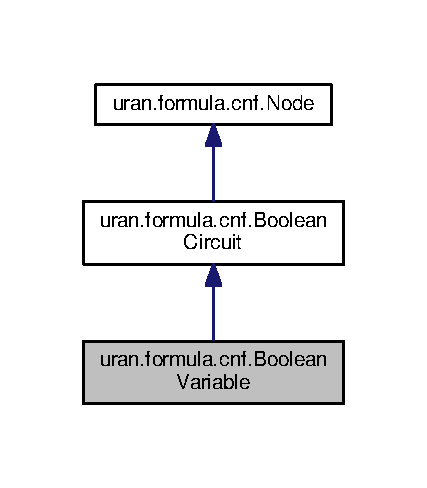
\includegraphics[width=205pt]{classuran_1_1formula_1_1cnf_1_1_boolean_variable__inherit__graph}
\end{center}
\end{figure}


Collaboration diagram for uran.\+formula.\+cnf.\+Boolean\+Variable\+:
\nopagebreak
\begin{figure}[H]
\begin{center}
\leavevmode
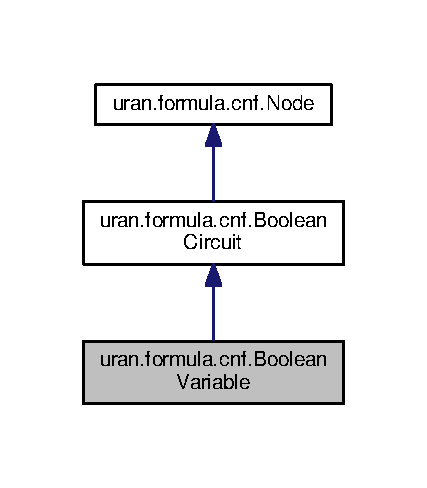
\includegraphics[width=205pt]{classuran_1_1formula_1_1cnf_1_1_boolean_variable__coll__graph}
\end{center}
\end{figure}
\subsection*{Public Member Functions}
\begin{DoxyCompactItemize}
\item 
\hyperlink{classuran_1_1formula_1_1cnf_1_1_boolean_variable_acc41e5e4e33ccc4db8e20ae3f1b23619}{Boolean\+Variable} (String name)
\item 
int \hyperlink{classuran_1_1formula_1_1cnf_1_1_boolean_variable_aacbd3bdf07826f1a0bc5dac94b0a3903}{hash\+Code} ()
\item 
String \hyperlink{classuran_1_1formula_1_1cnf_1_1_boolean_variable_ad309b8fb1955427b3962b013c8f78cc1}{alias} ()
\item 
String \hyperlink{classuran_1_1formula_1_1cnf_1_1_boolean_variable_ae1b00401cf7296fe52772a4f8b0899e0}{to\+String} ()
\item 
boolean \hyperlink{classuran_1_1formula_1_1cnf_1_1_boolean_variable_a8827aedaffa260fa107b3b2b5c59f197}{is\+Boolean\+Variable} ()
\item 
void \hyperlink{classuran_1_1formula_1_1cnf_1_1_boolean_variable_a910e2c688a7f9ad8e7f599a2f1df4b82}{accept} (\hyperlink{classuran_1_1formula_1_1cnf_1_1visitor_1_1_abstract_visitor}{Abstract\+Visitor} v)
\end{DoxyCompactItemize}
\subsection*{Additional Inherited Members}


\subsection{Detailed Description}


Definition at line 18 of file Boolean\+Variable.\+java.



\subsection{Constructor \& Destructor Documentation}
\hypertarget{classuran_1_1formula_1_1cnf_1_1_boolean_variable_acc41e5e4e33ccc4db8e20ae3f1b23619}{}\index{uran\+::formula\+::cnf\+::\+Boolean\+Variable@{uran\+::formula\+::cnf\+::\+Boolean\+Variable}!Boolean\+Variable@{Boolean\+Variable}}
\index{Boolean\+Variable@{Boolean\+Variable}!uran\+::formula\+::cnf\+::\+Boolean\+Variable@{uran\+::formula\+::cnf\+::\+Boolean\+Variable}}
\subsubsection[{Boolean\+Variable}]{\setlength{\rightskip}{0pt plus 5cm}uran.\+formula.\+cnf.\+Boolean\+Variable.\+Boolean\+Variable (
\begin{DoxyParamCaption}
\item[{String}]{name}
\end{DoxyParamCaption}
)\hspace{0.3cm}{\ttfamily [inline]}}\label{classuran_1_1formula_1_1cnf_1_1_boolean_variable_acc41e5e4e33ccc4db8e20ae3f1b23619}


Definition at line 21 of file Boolean\+Variable.\+java.



\subsection{Member Function Documentation}
\hypertarget{classuran_1_1formula_1_1cnf_1_1_boolean_variable_a910e2c688a7f9ad8e7f599a2f1df4b82}{}\index{uran\+::formula\+::cnf\+::\+Boolean\+Variable@{uran\+::formula\+::cnf\+::\+Boolean\+Variable}!accept@{accept}}
\index{accept@{accept}!uran\+::formula\+::cnf\+::\+Boolean\+Variable@{uran\+::formula\+::cnf\+::\+Boolean\+Variable}}
\subsubsection[{accept}]{\setlength{\rightskip}{0pt plus 5cm}void uran.\+formula.\+cnf.\+Boolean\+Variable.\+accept (
\begin{DoxyParamCaption}
\item[{{\bf Abstract\+Visitor}}]{v}
\end{DoxyParamCaption}
)\hspace{0.3cm}{\ttfamily [inline]}}\label{classuran_1_1formula_1_1cnf_1_1_boolean_variable_a910e2c688a7f9ad8e7f599a2f1df4b82}


Definition at line 40 of file Boolean\+Variable.\+java.

\hypertarget{classuran_1_1formula_1_1cnf_1_1_boolean_variable_ad309b8fb1955427b3962b013c8f78cc1}{}\index{uran\+::formula\+::cnf\+::\+Boolean\+Variable@{uran\+::formula\+::cnf\+::\+Boolean\+Variable}!alias@{alias}}
\index{alias@{alias}!uran\+::formula\+::cnf\+::\+Boolean\+Variable@{uran\+::formula\+::cnf\+::\+Boolean\+Variable}}
\subsubsection[{alias}]{\setlength{\rightskip}{0pt plus 5cm}String uran.\+formula.\+cnf.\+Boolean\+Variable.\+alias (
\begin{DoxyParamCaption}
{}
\end{DoxyParamCaption}
)\hspace{0.3cm}{\ttfamily [inline]}}\label{classuran_1_1formula_1_1cnf_1_1_boolean_variable_ad309b8fb1955427b3962b013c8f78cc1}


Definition at line 35 of file Boolean\+Variable.\+java.

\hypertarget{classuran_1_1formula_1_1cnf_1_1_boolean_variable_aacbd3bdf07826f1a0bc5dac94b0a3903}{}\index{uran\+::formula\+::cnf\+::\+Boolean\+Variable@{uran\+::formula\+::cnf\+::\+Boolean\+Variable}!hash\+Code@{hash\+Code}}
\index{hash\+Code@{hash\+Code}!uran\+::formula\+::cnf\+::\+Boolean\+Variable@{uran\+::formula\+::cnf\+::\+Boolean\+Variable}}
\subsubsection[{hash\+Code}]{\setlength{\rightskip}{0pt plus 5cm}int uran.\+formula.\+cnf.\+Boolean\+Variable.\+hash\+Code (
\begin{DoxyParamCaption}
{}
\end{DoxyParamCaption}
)\hspace{0.3cm}{\ttfamily [inline]}}\label{classuran_1_1formula_1_1cnf_1_1_boolean_variable_aacbd3bdf07826f1a0bc5dac94b0a3903}


Definition at line 24 of file Boolean\+Variable.\+java.

\hypertarget{classuran_1_1formula_1_1cnf_1_1_boolean_variable_a8827aedaffa260fa107b3b2b5c59f197}{}\index{uran\+::formula\+::cnf\+::\+Boolean\+Variable@{uran\+::formula\+::cnf\+::\+Boolean\+Variable}!is\+Boolean\+Variable@{is\+Boolean\+Variable}}
\index{is\+Boolean\+Variable@{is\+Boolean\+Variable}!uran\+::formula\+::cnf\+::\+Boolean\+Variable@{uran\+::formula\+::cnf\+::\+Boolean\+Variable}}
\subsubsection[{is\+Boolean\+Variable}]{\setlength{\rightskip}{0pt plus 5cm}boolean uran.\+formula.\+cnf.\+Boolean\+Variable.\+is\+Boolean\+Variable (
\begin{DoxyParamCaption}
{}
\end{DoxyParamCaption}
)\hspace{0.3cm}{\ttfamily [inline]}}\label{classuran_1_1formula_1_1cnf_1_1_boolean_variable_a8827aedaffa260fa107b3b2b5c59f197}


Definition at line 39 of file Boolean\+Variable.\+java.

\hypertarget{classuran_1_1formula_1_1cnf_1_1_boolean_variable_ae1b00401cf7296fe52772a4f8b0899e0}{}\index{uran\+::formula\+::cnf\+::\+Boolean\+Variable@{uran\+::formula\+::cnf\+::\+Boolean\+Variable}!to\+String@{to\+String}}
\index{to\+String@{to\+String}!uran\+::formula\+::cnf\+::\+Boolean\+Variable@{uran\+::formula\+::cnf\+::\+Boolean\+Variable}}
\subsubsection[{to\+String}]{\setlength{\rightskip}{0pt plus 5cm}String uran.\+formula.\+cnf.\+Boolean\+Variable.\+to\+String (
\begin{DoxyParamCaption}
{}
\end{DoxyParamCaption}
)\hspace{0.3cm}{\ttfamily [inline]}}\label{classuran_1_1formula_1_1cnf_1_1_boolean_variable_ae1b00401cf7296fe52772a4f8b0899e0}


Definition at line 36 of file Boolean\+Variable.\+java.



The documentation for this class was generated from the following file\+:\begin{DoxyCompactItemize}
\item 
/home/haowu/uran/src/uran/formula/cnf/\hyperlink{_boolean_variable_8java}{Boolean\+Variable.\+java}\end{DoxyCompactItemize}

\hypertarget{classuran_1_1formula_1_1_bool_literal}{}\section{uran.\+formula.\+Bool\+Literal Class Reference}
\label{classuran_1_1formula_1_1_bool_literal}\index{uran.\+formula.\+Bool\+Literal@{uran.\+formula.\+Bool\+Literal}}


Inheritance diagram for uran.\+formula.\+Bool\+Literal\+:
\nopagebreak
\begin{figure}[H]
\begin{center}
\leavevmode
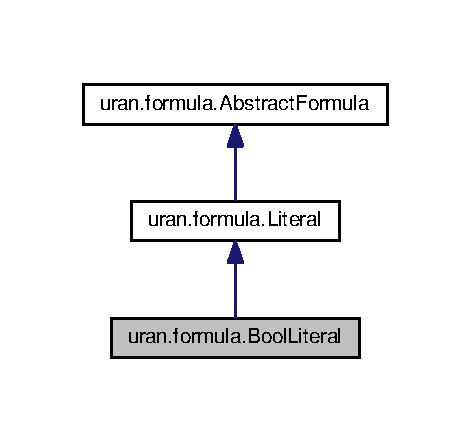
\includegraphics[width=226pt]{classuran_1_1formula_1_1_bool_literal__inherit__graph}
\end{center}
\end{figure}


Collaboration diagram for uran.\+formula.\+Bool\+Literal\+:
\nopagebreak
\begin{figure}[H]
\begin{center}
\leavevmode
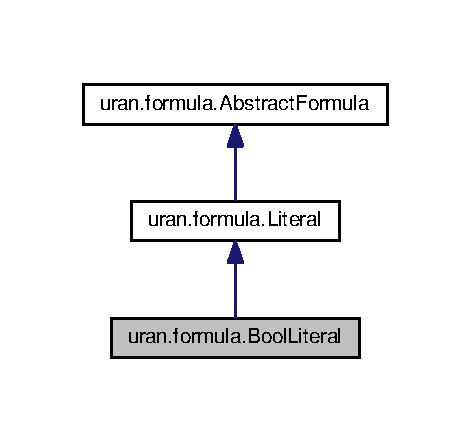
\includegraphics[width=226pt]{classuran_1_1formula_1_1_bool_literal__coll__graph}
\end{center}
\end{figure}
\subsection*{Public Member Functions}
\begin{DoxyCompactItemize}
\item 
\hyperlink{classuran_1_1formula_1_1_bool_literal_ac6066e2fcca3769785815be4dec819b9}{Bool\+Literal} ()
\item 
\hyperlink{classuran_1_1formula_1_1_bool_literal_af68639700ee15a8c658bfaace2ba691a}{Bool\+Literal} (\hyperlink{classuran_1_1formula_1_1value_1_1_bool_value}{Bool\+Value} v)
\item 
\hyperlink{classuran_1_1formula_1_1_bool_literal_a78102e1eda6c6c868aab6663fc6de03f}{Bool\+Literal} (boolean b)
\item 
boolean \hyperlink{classuran_1_1formula_1_1_bool_literal_a243c1c5df4f18c1bb68e2910efd7c4d0}{get\+Literal} ()
\item 
\hyperlink{classuran_1_1formula_1_1value_1_1_bool_value}{Bool\+Value} \hyperlink{classuran_1_1formula_1_1_bool_literal_a2f7f9e45f86a8a619a933cc309a29da8}{get\+Value} ()
\item 
String \hyperlink{classuran_1_1formula_1_1_bool_literal_ac0ed2eff11f5277ce7046a183f402604}{to\+String} ()
\item 
String \hyperlink{classuran_1_1formula_1_1_bool_literal_ac0d33bb85933baa6d946da255ab0f830}{to\+S\+M\+T2} ()
\item 
void \hyperlink{classuran_1_1formula_1_1_bool_literal_aaaf68f3020c254408ea56255e21a6d1c}{accept} (\hyperlink{classuran_1_1formula_1_1visitor_1_1_abstract_visitor}{Abstract\+Visitor} visitor)
\end{DoxyCompactItemize}


\subsection{Detailed Description}


Definition at line 18 of file Bool\+Literal.\+java.



\subsection{Constructor \& Destructor Documentation}
\hypertarget{classuran_1_1formula_1_1_bool_literal_ac6066e2fcca3769785815be4dec819b9}{}\index{uran\+::formula\+::\+Bool\+Literal@{uran\+::formula\+::\+Bool\+Literal}!Bool\+Literal@{Bool\+Literal}}
\index{Bool\+Literal@{Bool\+Literal}!uran\+::formula\+::\+Bool\+Literal@{uran\+::formula\+::\+Bool\+Literal}}
\subsubsection[{Bool\+Literal}]{\setlength{\rightskip}{0pt plus 5cm}uran.\+formula.\+Bool\+Literal.\+Bool\+Literal (
\begin{DoxyParamCaption}
{}
\end{DoxyParamCaption}
)\hspace{0.3cm}{\ttfamily [inline]}}\label{classuran_1_1formula_1_1_bool_literal_ac6066e2fcca3769785815be4dec819b9}


Definition at line 21 of file Bool\+Literal.\+java.

\hypertarget{classuran_1_1formula_1_1_bool_literal_af68639700ee15a8c658bfaace2ba691a}{}\index{uran\+::formula\+::\+Bool\+Literal@{uran\+::formula\+::\+Bool\+Literal}!Bool\+Literal@{Bool\+Literal}}
\index{Bool\+Literal@{Bool\+Literal}!uran\+::formula\+::\+Bool\+Literal@{uran\+::formula\+::\+Bool\+Literal}}
\subsubsection[{Bool\+Literal}]{\setlength{\rightskip}{0pt plus 5cm}uran.\+formula.\+Bool\+Literal.\+Bool\+Literal (
\begin{DoxyParamCaption}
\item[{{\bf Bool\+Value}}]{v}
\end{DoxyParamCaption}
)\hspace{0.3cm}{\ttfamily [inline]}}\label{classuran_1_1formula_1_1_bool_literal_af68639700ee15a8c658bfaace2ba691a}


Definition at line 26 of file Bool\+Literal.\+java.

\hypertarget{classuran_1_1formula_1_1_bool_literal_a78102e1eda6c6c868aab6663fc6de03f}{}\index{uran\+::formula\+::\+Bool\+Literal@{uran\+::formula\+::\+Bool\+Literal}!Bool\+Literal@{Bool\+Literal}}
\index{Bool\+Literal@{Bool\+Literal}!uran\+::formula\+::\+Bool\+Literal@{uran\+::formula\+::\+Bool\+Literal}}
\subsubsection[{Bool\+Literal}]{\setlength{\rightskip}{0pt plus 5cm}uran.\+formula.\+Bool\+Literal.\+Bool\+Literal (
\begin{DoxyParamCaption}
\item[{boolean}]{b}
\end{DoxyParamCaption}
)\hspace{0.3cm}{\ttfamily [inline]}}\label{classuran_1_1formula_1_1_bool_literal_a78102e1eda6c6c868aab6663fc6de03f}


Definition at line 30 of file Bool\+Literal.\+java.



\subsection{Member Function Documentation}
\hypertarget{classuran_1_1formula_1_1_bool_literal_aaaf68f3020c254408ea56255e21a6d1c}{}\index{uran\+::formula\+::\+Bool\+Literal@{uran\+::formula\+::\+Bool\+Literal}!accept@{accept}}
\index{accept@{accept}!uran\+::formula\+::\+Bool\+Literal@{uran\+::formula\+::\+Bool\+Literal}}
\subsubsection[{accept}]{\setlength{\rightskip}{0pt plus 5cm}void uran.\+formula.\+Bool\+Literal.\+accept (
\begin{DoxyParamCaption}
\item[{{\bf Abstract\+Visitor}}]{visitor}
\end{DoxyParamCaption}
)\hspace{0.3cm}{\ttfamily [inline]}}\label{classuran_1_1formula_1_1_bool_literal_aaaf68f3020c254408ea56255e21a6d1c}


Definition at line 50 of file Bool\+Literal.\+java.

\hypertarget{classuran_1_1formula_1_1_bool_literal_a243c1c5df4f18c1bb68e2910efd7c4d0}{}\index{uran\+::formula\+::\+Bool\+Literal@{uran\+::formula\+::\+Bool\+Literal}!get\+Literal@{get\+Literal}}
\index{get\+Literal@{get\+Literal}!uran\+::formula\+::\+Bool\+Literal@{uran\+::formula\+::\+Bool\+Literal}}
\subsubsection[{get\+Literal}]{\setlength{\rightskip}{0pt plus 5cm}boolean uran.\+formula.\+Bool\+Literal.\+get\+Literal (
\begin{DoxyParamCaption}
{}
\end{DoxyParamCaption}
)\hspace{0.3cm}{\ttfamily [inline]}}\label{classuran_1_1formula_1_1_bool_literal_a243c1c5df4f18c1bb68e2910efd7c4d0}


Definition at line 34 of file Bool\+Literal.\+java.

\hypertarget{classuran_1_1formula_1_1_bool_literal_a2f7f9e45f86a8a619a933cc309a29da8}{}\index{uran\+::formula\+::\+Bool\+Literal@{uran\+::formula\+::\+Bool\+Literal}!get\+Value@{get\+Value}}
\index{get\+Value@{get\+Value}!uran\+::formula\+::\+Bool\+Literal@{uran\+::formula\+::\+Bool\+Literal}}
\subsubsection[{get\+Value}]{\setlength{\rightskip}{0pt plus 5cm}{\bf Bool\+Value} uran.\+formula.\+Bool\+Literal.\+get\+Value (
\begin{DoxyParamCaption}
{}
\end{DoxyParamCaption}
)\hspace{0.3cm}{\ttfamily [inline]}}\label{classuran_1_1formula_1_1_bool_literal_a2f7f9e45f86a8a619a933cc309a29da8}


Definition at line 38 of file Bool\+Literal.\+java.

\hypertarget{classuran_1_1formula_1_1_bool_literal_ac0d33bb85933baa6d946da255ab0f830}{}\index{uran\+::formula\+::\+Bool\+Literal@{uran\+::formula\+::\+Bool\+Literal}!to\+S\+M\+T2@{to\+S\+M\+T2}}
\index{to\+S\+M\+T2@{to\+S\+M\+T2}!uran\+::formula\+::\+Bool\+Literal@{uran\+::formula\+::\+Bool\+Literal}}
\subsubsection[{to\+S\+M\+T2}]{\setlength{\rightskip}{0pt plus 5cm}String uran.\+formula.\+Bool\+Literal.\+to\+S\+M\+T2 (
\begin{DoxyParamCaption}
{}
\end{DoxyParamCaption}
)\hspace{0.3cm}{\ttfamily [inline]}}\label{classuran_1_1formula_1_1_bool_literal_ac0d33bb85933baa6d946da255ab0f830}


Definition at line 47 of file Bool\+Literal.\+java.

\hypertarget{classuran_1_1formula_1_1_bool_literal_ac0ed2eff11f5277ce7046a183f402604}{}\index{uran\+::formula\+::\+Bool\+Literal@{uran\+::formula\+::\+Bool\+Literal}!to\+String@{to\+String}}
\index{to\+String@{to\+String}!uran\+::formula\+::\+Bool\+Literal@{uran\+::formula\+::\+Bool\+Literal}}
\subsubsection[{to\+String}]{\setlength{\rightskip}{0pt plus 5cm}String uran.\+formula.\+Bool\+Literal.\+to\+String (
\begin{DoxyParamCaption}
{}
\end{DoxyParamCaption}
)\hspace{0.3cm}{\ttfamily [inline]}}\label{classuran_1_1formula_1_1_bool_literal_ac0ed2eff11f5277ce7046a183f402604}


Definition at line 42 of file Bool\+Literal.\+java.



The documentation for this class was generated from the following file\+:\begin{DoxyCompactItemize}
\item 
/home/haowu/uran/src/uran/formula/\hyperlink{_bool_literal_8java}{Bool\+Literal.\+java}\end{DoxyCompactItemize}

\hypertarget{classuran_1_1formula_1_1value_1_1_bool_value}{}\section{uran.\+formula.\+value.\+Bool\+Value Class Reference}
\label{classuran_1_1formula_1_1value_1_1_bool_value}\index{uran.\+formula.\+value.\+Bool\+Value@{uran.\+formula.\+value.\+Bool\+Value}}


Inheritance diagram for uran.\+formula.\+value.\+Bool\+Value\+:
\nopagebreak
\begin{figure}[H]
\begin{center}
\leavevmode
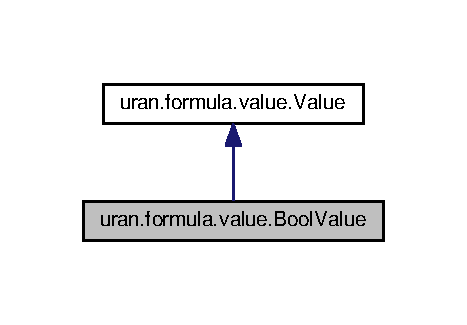
\includegraphics[width=224pt]{classuran_1_1formula_1_1value_1_1_bool_value__inherit__graph}
\end{center}
\end{figure}


Collaboration diagram for uran.\+formula.\+value.\+Bool\+Value\+:
\nopagebreak
\begin{figure}[H]
\begin{center}
\leavevmode
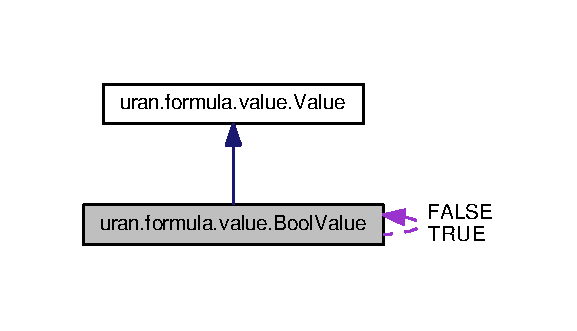
\includegraphics[width=277pt]{classuran_1_1formula_1_1value_1_1_bool_value__coll__graph}
\end{center}
\end{figure}
\subsection*{Public Member Functions}
\begin{DoxyCompactItemize}
\item 
\hyperlink{classuran_1_1formula_1_1value_1_1_bool_value_ab75d7d7bd1d808aa9332300d345a6392}{Bool\+Value} ()
\item 
\hyperlink{classuran_1_1formula_1_1value_1_1_bool_value_a07f50b1039186e22dd580052d8af77e4}{Bool\+Value} (boolean b)
\item 
boolean \hyperlink{classuran_1_1formula_1_1value_1_1_bool_value_a3793758209ff1ab589e0d82b79161791}{get\+Value} ()
\item 
void \hyperlink{classuran_1_1formula_1_1value_1_1_bool_value_a01d8351e393778f739c3628a5b29dde3}{set\+Value} (boolean n)
\item 
boolean \hyperlink{classuran_1_1formula_1_1value_1_1_bool_value_af8bccd2ef7c5d744e19252a0271b7cfa}{Is\+Bool} ()
\item 
String \hyperlink{classuran_1_1formula_1_1value_1_1_bool_value_af60d21a25ebdfb22998f474a46db089e}{to\+String} ()
\end{DoxyCompactItemize}
\subsection*{Static Public Attributes}
\begin{DoxyCompactItemize}
\item 
static final \hyperlink{classuran_1_1formula_1_1value_1_1_bool_value}{Bool\+Value} \hyperlink{classuran_1_1formula_1_1value_1_1_bool_value_aa3ce9a9ee8cda8144593e4c4d54151b2}{T\+R\+U\+E} = new \hyperlink{classuran_1_1formula_1_1value_1_1_bool_value}{Bool\+Value}(true)
\item 
static final \hyperlink{classuran_1_1formula_1_1value_1_1_bool_value}{Bool\+Value} \hyperlink{classuran_1_1formula_1_1value_1_1_bool_value_aa95a1b324774790da1c3aea1993baf73}{F\+A\+L\+S\+E} = new \hyperlink{classuran_1_1formula_1_1value_1_1_bool_value}{Bool\+Value}(false)
\end{DoxyCompactItemize}


\subsection{Detailed Description}


Definition at line 15 of file Bool\+Value.\+java.



\subsection{Constructor \& Destructor Documentation}
\hypertarget{classuran_1_1formula_1_1value_1_1_bool_value_ab75d7d7bd1d808aa9332300d345a6392}{}\index{uran\+::formula\+::value\+::\+Bool\+Value@{uran\+::formula\+::value\+::\+Bool\+Value}!Bool\+Value@{Bool\+Value}}
\index{Bool\+Value@{Bool\+Value}!uran\+::formula\+::value\+::\+Bool\+Value@{uran\+::formula\+::value\+::\+Bool\+Value}}
\subsubsection[{Bool\+Value}]{\setlength{\rightskip}{0pt plus 5cm}uran.\+formula.\+value.\+Bool\+Value.\+Bool\+Value (
\begin{DoxyParamCaption}
{}
\end{DoxyParamCaption}
)\hspace{0.3cm}{\ttfamily [inline]}}\label{classuran_1_1formula_1_1value_1_1_bool_value_ab75d7d7bd1d808aa9332300d345a6392}


Definition at line 19 of file Bool\+Value.\+java.

\hypertarget{classuran_1_1formula_1_1value_1_1_bool_value_a07f50b1039186e22dd580052d8af77e4}{}\index{uran\+::formula\+::value\+::\+Bool\+Value@{uran\+::formula\+::value\+::\+Bool\+Value}!Bool\+Value@{Bool\+Value}}
\index{Bool\+Value@{Bool\+Value}!uran\+::formula\+::value\+::\+Bool\+Value@{uran\+::formula\+::value\+::\+Bool\+Value}}
\subsubsection[{Bool\+Value}]{\setlength{\rightskip}{0pt plus 5cm}uran.\+formula.\+value.\+Bool\+Value.\+Bool\+Value (
\begin{DoxyParamCaption}
\item[{boolean}]{b}
\end{DoxyParamCaption}
)\hspace{0.3cm}{\ttfamily [inline]}}\label{classuran_1_1formula_1_1value_1_1_bool_value_a07f50b1039186e22dd580052d8af77e4}


Definition at line 20 of file Bool\+Value.\+java.



\subsection{Member Function Documentation}
\hypertarget{classuran_1_1formula_1_1value_1_1_bool_value_a3793758209ff1ab589e0d82b79161791}{}\index{uran\+::formula\+::value\+::\+Bool\+Value@{uran\+::formula\+::value\+::\+Bool\+Value}!get\+Value@{get\+Value}}
\index{get\+Value@{get\+Value}!uran\+::formula\+::value\+::\+Bool\+Value@{uran\+::formula\+::value\+::\+Bool\+Value}}
\subsubsection[{get\+Value}]{\setlength{\rightskip}{0pt plus 5cm}boolean uran.\+formula.\+value.\+Bool\+Value.\+get\+Value (
\begin{DoxyParamCaption}
{}
\end{DoxyParamCaption}
)\hspace{0.3cm}{\ttfamily [inline]}}\label{classuran_1_1formula_1_1value_1_1_bool_value_a3793758209ff1ab589e0d82b79161791}


Definition at line 21 of file Bool\+Value.\+java.

\hypertarget{classuran_1_1formula_1_1value_1_1_bool_value_af8bccd2ef7c5d744e19252a0271b7cfa}{}\index{uran\+::formula\+::value\+::\+Bool\+Value@{uran\+::formula\+::value\+::\+Bool\+Value}!Is\+Bool@{Is\+Bool}}
\index{Is\+Bool@{Is\+Bool}!uran\+::formula\+::value\+::\+Bool\+Value@{uran\+::formula\+::value\+::\+Bool\+Value}}
\subsubsection[{Is\+Bool}]{\setlength{\rightskip}{0pt plus 5cm}boolean uran.\+formula.\+value.\+Bool\+Value.\+Is\+Bool (
\begin{DoxyParamCaption}
{}
\end{DoxyParamCaption}
)\hspace{0.3cm}{\ttfamily [inline]}}\label{classuran_1_1formula_1_1value_1_1_bool_value_af8bccd2ef7c5d744e19252a0271b7cfa}


Definition at line 23 of file Bool\+Value.\+java.

\hypertarget{classuran_1_1formula_1_1value_1_1_bool_value_a01d8351e393778f739c3628a5b29dde3}{}\index{uran\+::formula\+::value\+::\+Bool\+Value@{uran\+::formula\+::value\+::\+Bool\+Value}!set\+Value@{set\+Value}}
\index{set\+Value@{set\+Value}!uran\+::formula\+::value\+::\+Bool\+Value@{uran\+::formula\+::value\+::\+Bool\+Value}}
\subsubsection[{set\+Value}]{\setlength{\rightskip}{0pt plus 5cm}void uran.\+formula.\+value.\+Bool\+Value.\+set\+Value (
\begin{DoxyParamCaption}
\item[{boolean}]{n}
\end{DoxyParamCaption}
)\hspace{0.3cm}{\ttfamily [inline]}}\label{classuran_1_1formula_1_1value_1_1_bool_value_a01d8351e393778f739c3628a5b29dde3}


Definition at line 22 of file Bool\+Value.\+java.

\hypertarget{classuran_1_1formula_1_1value_1_1_bool_value_af60d21a25ebdfb22998f474a46db089e}{}\index{uran\+::formula\+::value\+::\+Bool\+Value@{uran\+::formula\+::value\+::\+Bool\+Value}!to\+String@{to\+String}}
\index{to\+String@{to\+String}!uran\+::formula\+::value\+::\+Bool\+Value@{uran\+::formula\+::value\+::\+Bool\+Value}}
\subsubsection[{to\+String}]{\setlength{\rightskip}{0pt plus 5cm}String uran.\+formula.\+value.\+Bool\+Value.\+to\+String (
\begin{DoxyParamCaption}
{}
\end{DoxyParamCaption}
)\hspace{0.3cm}{\ttfamily [inline]}}\label{classuran_1_1formula_1_1value_1_1_bool_value_af60d21a25ebdfb22998f474a46db089e}


Definition at line 24 of file Bool\+Value.\+java.



\subsection{Member Data Documentation}
\hypertarget{classuran_1_1formula_1_1value_1_1_bool_value_aa95a1b324774790da1c3aea1993baf73}{}\index{uran\+::formula\+::value\+::\+Bool\+Value@{uran\+::formula\+::value\+::\+Bool\+Value}!F\+A\+L\+S\+E@{F\+A\+L\+S\+E}}
\index{F\+A\+L\+S\+E@{F\+A\+L\+S\+E}!uran\+::formula\+::value\+::\+Bool\+Value@{uran\+::formula\+::value\+::\+Bool\+Value}}
\subsubsection[{F\+A\+L\+S\+E}]{\setlength{\rightskip}{0pt plus 5cm}final {\bf Bool\+Value} uran.\+formula.\+value.\+Bool\+Value.\+F\+A\+L\+S\+E = new {\bf Bool\+Value}(false)\hspace{0.3cm}{\ttfamily [static]}}\label{classuran_1_1formula_1_1value_1_1_bool_value_aa95a1b324774790da1c3aea1993baf73}


Definition at line 17 of file Bool\+Value.\+java.

\hypertarget{classuran_1_1formula_1_1value_1_1_bool_value_aa3ce9a9ee8cda8144593e4c4d54151b2}{}\index{uran\+::formula\+::value\+::\+Bool\+Value@{uran\+::formula\+::value\+::\+Bool\+Value}!T\+R\+U\+E@{T\+R\+U\+E}}
\index{T\+R\+U\+E@{T\+R\+U\+E}!uran\+::formula\+::value\+::\+Bool\+Value@{uran\+::formula\+::value\+::\+Bool\+Value}}
\subsubsection[{T\+R\+U\+E}]{\setlength{\rightskip}{0pt plus 5cm}final {\bf Bool\+Value} uran.\+formula.\+value.\+Bool\+Value.\+T\+R\+U\+E = new {\bf Bool\+Value}(true)\hspace{0.3cm}{\ttfamily [static]}}\label{classuran_1_1formula_1_1value_1_1_bool_value_aa3ce9a9ee8cda8144593e4c4d54151b2}


Definition at line 16 of file Bool\+Value.\+java.



The documentation for this class was generated from the following file\+:\begin{DoxyCompactItemize}
\item 
/home/haowu/uran/src/uran/formula/value/\hyperlink{_bool_value_8java}{Bool\+Value.\+java}\end{DoxyCompactItemize}

\hypertarget{classuran_1_1formula_1_1cnf_1_1_c_n_f_translator}{}\section{uran.\+formula.\+cnf.\+C\+N\+F\+Translator Class Reference}
\label{classuran_1_1formula_1_1cnf_1_1_c_n_f_translator}\index{uran.\+formula.\+cnf.\+C\+N\+F\+Translator@{uran.\+formula.\+cnf.\+C\+N\+F\+Translator}}


Inheritance diagram for uran.\+formula.\+cnf.\+C\+N\+F\+Translator\+:
\nopagebreak
\begin{figure}[H]
\begin{center}
\leavevmode
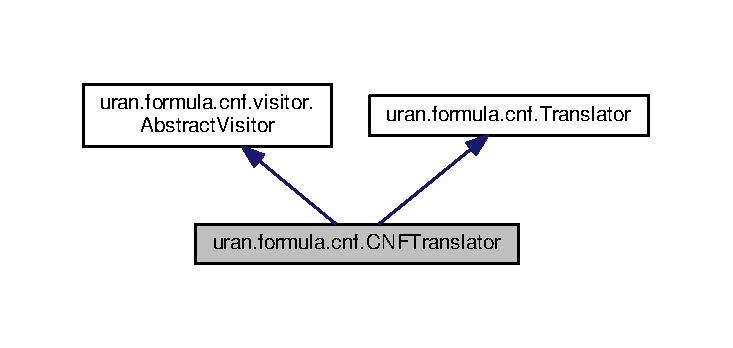
\includegraphics[width=350pt]{classuran_1_1formula_1_1cnf_1_1_c_n_f_translator__inherit__graph}
\end{center}
\end{figure}


Collaboration diagram for uran.\+formula.\+cnf.\+C\+N\+F\+Translator\+:
\nopagebreak
\begin{figure}[H]
\begin{center}
\leavevmode
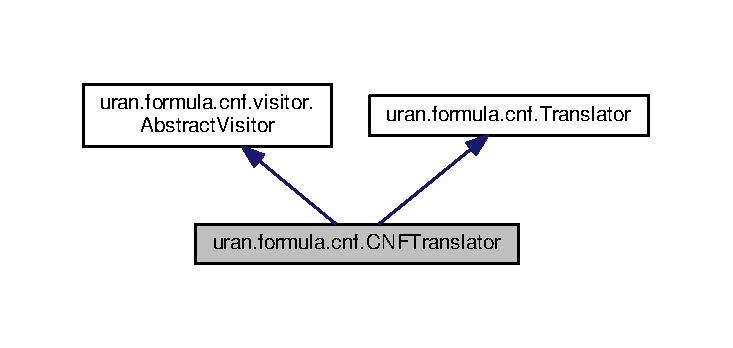
\includegraphics[width=350pt]{classuran_1_1formula_1_1cnf_1_1_c_n_f_translator__coll__graph}
\end{center}
\end{figure}
\subsection*{Public Member Functions}
\begin{DoxyCompactItemize}
\item 
\hyperlink{classuran_1_1formula_1_1cnf_1_1_c_n_f_translator_ae56a0dc54a2ef3be4ddb496b57ba224d}{C\+N\+F\+Translator} (\hyperlink{classuran_1_1formula_1_1cnf_1_1_boolean_circuit}{Boolean\+Circuit} c, String filename)
\item 
\hyperlink{classuran_1_1formula_1_1cnf_1_1_c_n_f_translator_a9f75243260e3af2aebe1e1466bbe5996}{C\+N\+F\+Translator} (\hyperlink{classuran_1_1formula_1_1cnf_1_1_boolean_circuit}{Boolean\+Circuit}\mbox{[}$\,$\mbox{]} c, String filename)
\item 
void \hyperlink{classuran_1_1formula_1_1cnf_1_1_c_n_f_translator_a8cfa090e193eeb2a77a013a1d462576e}{translate} ()
\item 
void \hyperlink{classuran_1_1formula_1_1cnf_1_1_c_n_f_translator_a9d52eae57163cb730e343c1071cf0091}{translate} (\hyperlink{classuran_1_1formula_1_1cnf_1_1_boolean_circuit}{Boolean\+Circuit} c)
\item 
void \hyperlink{classuran_1_1formula_1_1cnf_1_1_c_n_f_translator_a3248f27b474b29e715e86fa4accf99eb}{visit} (\hyperlink{classuran_1_1formula_1_1cnf_1_1_binary_gate}{Binary\+Gate} b)
\item 
void \hyperlink{classuran_1_1formula_1_1cnf_1_1_c_n_f_translator_a9e35ea3cb123b609d8ea5eb28cb8a582}{visit} (\hyperlink{classuran_1_1formula_1_1cnf_1_1_boolean_variable}{Boolean\+Variable} v)
\item 
void \hyperlink{classuran_1_1formula_1_1cnf_1_1_c_n_f_translator_ae1e16723069c2bc4f493a7d04dff4186}{visit} (\hyperlink{classuran_1_1formula_1_1cnf_1_1_not_gate}{Not\+Gate} n)
\item 
void \hyperlink{classuran_1_1formula_1_1cnf_1_1_c_n_f_translator_a647b4754a2c7cedd0cb452463927efff}{new\+Variable} (\hyperlink{classuran_1_1formula_1_1cnf_1_1_boolean_circuit}{Boolean\+Circuit} c)
\item 
void \hyperlink{classuran_1_1formula_1_1cnf_1_1_c_n_f_translator_a623c2f1b2e56c46bbbc3a289aaba0528}{generate} ()
\item 
long \hyperlink{classuran_1_1formula_1_1cnf_1_1_c_n_f_translator_af16fa6b850daf26021eb229b6b5f52ea}{no\+Of\+Variables} ()
\item 
long \hyperlink{classuran_1_1formula_1_1cnf_1_1_c_n_f_translator_a65be5754fdf4c8459126a5941116f0d5}{no\+Of\+Clauses} ()
\end{DoxyCompactItemize}


\subsection{Detailed Description}


Definition at line 31 of file C\+N\+F\+Translator.\+java.



\subsection{Constructor \& Destructor Documentation}
\hypertarget{classuran_1_1formula_1_1cnf_1_1_c_n_f_translator_ae56a0dc54a2ef3be4ddb496b57ba224d}{}\index{uran\+::formula\+::cnf\+::\+C\+N\+F\+Translator@{uran\+::formula\+::cnf\+::\+C\+N\+F\+Translator}!C\+N\+F\+Translator@{C\+N\+F\+Translator}}
\index{C\+N\+F\+Translator@{C\+N\+F\+Translator}!uran\+::formula\+::cnf\+::\+C\+N\+F\+Translator@{uran\+::formula\+::cnf\+::\+C\+N\+F\+Translator}}
\subsubsection[{C\+N\+F\+Translator}]{\setlength{\rightskip}{0pt plus 5cm}uran.\+formula.\+cnf.\+C\+N\+F\+Translator.\+C\+N\+F\+Translator (
\begin{DoxyParamCaption}
\item[{{\bf Boolean\+Circuit}}]{c, }
\item[{String}]{filename}
\end{DoxyParamCaption}
)\hspace{0.3cm}{\ttfamily [inline]}}\label{classuran_1_1formula_1_1cnf_1_1_c_n_f_translator_ae56a0dc54a2ef3be4ddb496b57ba224d}


Definition at line 44 of file C\+N\+F\+Translator.\+java.

\hypertarget{classuran_1_1formula_1_1cnf_1_1_c_n_f_translator_a9f75243260e3af2aebe1e1466bbe5996}{}\index{uran\+::formula\+::cnf\+::\+C\+N\+F\+Translator@{uran\+::formula\+::cnf\+::\+C\+N\+F\+Translator}!C\+N\+F\+Translator@{C\+N\+F\+Translator}}
\index{C\+N\+F\+Translator@{C\+N\+F\+Translator}!uran\+::formula\+::cnf\+::\+C\+N\+F\+Translator@{uran\+::formula\+::cnf\+::\+C\+N\+F\+Translator}}
\subsubsection[{C\+N\+F\+Translator}]{\setlength{\rightskip}{0pt plus 5cm}uran.\+formula.\+cnf.\+C\+N\+F\+Translator.\+C\+N\+F\+Translator (
\begin{DoxyParamCaption}
\item[{{\bf Boolean\+Circuit}\mbox{[}$\,$\mbox{]}}]{c, }
\item[{String}]{filename}
\end{DoxyParamCaption}
)\hspace{0.3cm}{\ttfamily [inline]}}\label{classuran_1_1formula_1_1cnf_1_1_c_n_f_translator_a9f75243260e3af2aebe1e1466bbe5996}


Definition at line 52 of file C\+N\+F\+Translator.\+java.



\subsection{Member Function Documentation}
\hypertarget{classuran_1_1formula_1_1cnf_1_1_c_n_f_translator_a623c2f1b2e56c46bbbc3a289aaba0528}{}\index{uran\+::formula\+::cnf\+::\+C\+N\+F\+Translator@{uran\+::formula\+::cnf\+::\+C\+N\+F\+Translator}!generate@{generate}}
\index{generate@{generate}!uran\+::formula\+::cnf\+::\+C\+N\+F\+Translator@{uran\+::formula\+::cnf\+::\+C\+N\+F\+Translator}}
\subsubsection[{generate}]{\setlength{\rightskip}{0pt plus 5cm}void uran.\+formula.\+cnf.\+C\+N\+F\+Translator.\+generate (
\begin{DoxyParamCaption}
{}
\end{DoxyParamCaption}
)\hspace{0.3cm}{\ttfamily [inline]}}\label{classuran_1_1formula_1_1cnf_1_1_c_n_f_translator_a623c2f1b2e56c46bbbc3a289aaba0528}


Definition at line 293 of file C\+N\+F\+Translator.\+java.

\hypertarget{classuran_1_1formula_1_1cnf_1_1_c_n_f_translator_a647b4754a2c7cedd0cb452463927efff}{}\index{uran\+::formula\+::cnf\+::\+C\+N\+F\+Translator@{uran\+::formula\+::cnf\+::\+C\+N\+F\+Translator}!new\+Variable@{new\+Variable}}
\index{new\+Variable@{new\+Variable}!uran\+::formula\+::cnf\+::\+C\+N\+F\+Translator@{uran\+::formula\+::cnf\+::\+C\+N\+F\+Translator}}
\subsubsection[{new\+Variable}]{\setlength{\rightskip}{0pt plus 5cm}void uran.\+formula.\+cnf.\+C\+N\+F\+Translator.\+new\+Variable (
\begin{DoxyParamCaption}
\item[{{\bf Boolean\+Circuit}}]{c}
\end{DoxyParamCaption}
)\hspace{0.3cm}{\ttfamily [inline]}}\label{classuran_1_1formula_1_1cnf_1_1_c_n_f_translator_a647b4754a2c7cedd0cb452463927efff}


Definition at line 252 of file C\+N\+F\+Translator.\+java.

\hypertarget{classuran_1_1formula_1_1cnf_1_1_c_n_f_translator_a65be5754fdf4c8459126a5941116f0d5}{}\index{uran\+::formula\+::cnf\+::\+C\+N\+F\+Translator@{uran\+::formula\+::cnf\+::\+C\+N\+F\+Translator}!no\+Of\+Clauses@{no\+Of\+Clauses}}
\index{no\+Of\+Clauses@{no\+Of\+Clauses}!uran\+::formula\+::cnf\+::\+C\+N\+F\+Translator@{uran\+::formula\+::cnf\+::\+C\+N\+F\+Translator}}
\subsubsection[{no\+Of\+Clauses}]{\setlength{\rightskip}{0pt plus 5cm}long uran.\+formula.\+cnf.\+C\+N\+F\+Translator.\+no\+Of\+Clauses (
\begin{DoxyParamCaption}
{}
\end{DoxyParamCaption}
)\hspace{0.3cm}{\ttfamily [inline]}}\label{classuran_1_1formula_1_1cnf_1_1_c_n_f_translator_a65be5754fdf4c8459126a5941116f0d5}


Definition at line 307 of file C\+N\+F\+Translator.\+java.

\hypertarget{classuran_1_1formula_1_1cnf_1_1_c_n_f_translator_af16fa6b850daf26021eb229b6b5f52ea}{}\index{uran\+::formula\+::cnf\+::\+C\+N\+F\+Translator@{uran\+::formula\+::cnf\+::\+C\+N\+F\+Translator}!no\+Of\+Variables@{no\+Of\+Variables}}
\index{no\+Of\+Variables@{no\+Of\+Variables}!uran\+::formula\+::cnf\+::\+C\+N\+F\+Translator@{uran\+::formula\+::cnf\+::\+C\+N\+F\+Translator}}
\subsubsection[{no\+Of\+Variables}]{\setlength{\rightskip}{0pt plus 5cm}long uran.\+formula.\+cnf.\+C\+N\+F\+Translator.\+no\+Of\+Variables (
\begin{DoxyParamCaption}
{}
\end{DoxyParamCaption}
)\hspace{0.3cm}{\ttfamily [inline]}}\label{classuran_1_1formula_1_1cnf_1_1_c_n_f_translator_af16fa6b850daf26021eb229b6b5f52ea}


Definition at line 306 of file C\+N\+F\+Translator.\+java.

\hypertarget{classuran_1_1formula_1_1cnf_1_1_c_n_f_translator_a8cfa090e193eeb2a77a013a1d462576e}{}\index{uran\+::formula\+::cnf\+::\+C\+N\+F\+Translator@{uran\+::formula\+::cnf\+::\+C\+N\+F\+Translator}!translate@{translate}}
\index{translate@{translate}!uran\+::formula\+::cnf\+::\+C\+N\+F\+Translator@{uran\+::formula\+::cnf\+::\+C\+N\+F\+Translator}}
\subsubsection[{translate}]{\setlength{\rightskip}{0pt plus 5cm}void uran.\+formula.\+cnf.\+C\+N\+F\+Translator.\+translate (
\begin{DoxyParamCaption}
{}
\end{DoxyParamCaption}
)\hspace{0.3cm}{\ttfamily [inline]}}\label{classuran_1_1formula_1_1cnf_1_1_c_n_f_translator_a8cfa090e193eeb2a77a013a1d462576e}


Implements \hyperlink{interfaceuran_1_1formula_1_1cnf_1_1_translator_a55ca28e7487e311573b3593ced70d634}{uran.\+formula.\+cnf.\+Translator}.



Definition at line 59 of file C\+N\+F\+Translator.\+java.

\hypertarget{classuran_1_1formula_1_1cnf_1_1_c_n_f_translator_a9d52eae57163cb730e343c1071cf0091}{}\index{uran\+::formula\+::cnf\+::\+C\+N\+F\+Translator@{uran\+::formula\+::cnf\+::\+C\+N\+F\+Translator}!translate@{translate}}
\index{translate@{translate}!uran\+::formula\+::cnf\+::\+C\+N\+F\+Translator@{uran\+::formula\+::cnf\+::\+C\+N\+F\+Translator}}
\subsubsection[{translate}]{\setlength{\rightskip}{0pt plus 5cm}void uran.\+formula.\+cnf.\+C\+N\+F\+Translator.\+translate (
\begin{DoxyParamCaption}
\item[{{\bf Boolean\+Circuit}}]{c}
\end{DoxyParamCaption}
)\hspace{0.3cm}{\ttfamily [inline]}}\label{classuran_1_1formula_1_1cnf_1_1_c_n_f_translator_a9d52eae57163cb730e343c1071cf0091}


Definition at line 78 of file C\+N\+F\+Translator.\+java.

\hypertarget{classuran_1_1formula_1_1cnf_1_1_c_n_f_translator_a3248f27b474b29e715e86fa4accf99eb}{}\index{uran\+::formula\+::cnf\+::\+C\+N\+F\+Translator@{uran\+::formula\+::cnf\+::\+C\+N\+F\+Translator}!visit@{visit}}
\index{visit@{visit}!uran\+::formula\+::cnf\+::\+C\+N\+F\+Translator@{uran\+::formula\+::cnf\+::\+C\+N\+F\+Translator}}
\subsubsection[{visit}]{\setlength{\rightskip}{0pt plus 5cm}void uran.\+formula.\+cnf.\+C\+N\+F\+Translator.\+visit (
\begin{DoxyParamCaption}
\item[{{\bf Binary\+Gate}}]{b}
\end{DoxyParamCaption}
)\hspace{0.3cm}{\ttfamily [inline]}}\label{classuran_1_1formula_1_1cnf_1_1_c_n_f_translator_a3248f27b474b29e715e86fa4accf99eb}


Definition at line 92 of file C\+N\+F\+Translator.\+java.

\hypertarget{classuran_1_1formula_1_1cnf_1_1_c_n_f_translator_a9e35ea3cb123b609d8ea5eb28cb8a582}{}\index{uran\+::formula\+::cnf\+::\+C\+N\+F\+Translator@{uran\+::formula\+::cnf\+::\+C\+N\+F\+Translator}!visit@{visit}}
\index{visit@{visit}!uran\+::formula\+::cnf\+::\+C\+N\+F\+Translator@{uran\+::formula\+::cnf\+::\+C\+N\+F\+Translator}}
\subsubsection[{visit}]{\setlength{\rightskip}{0pt plus 5cm}void uran.\+formula.\+cnf.\+C\+N\+F\+Translator.\+visit (
\begin{DoxyParamCaption}
\item[{{\bf Boolean\+Variable}}]{v}
\end{DoxyParamCaption}
)\hspace{0.3cm}{\ttfamily [inline]}}\label{classuran_1_1formula_1_1cnf_1_1_c_n_f_translator_a9e35ea3cb123b609d8ea5eb28cb8a582}


Definition at line 240 of file C\+N\+F\+Translator.\+java.

\hypertarget{classuran_1_1formula_1_1cnf_1_1_c_n_f_translator_ae1e16723069c2bc4f493a7d04dff4186}{}\index{uran\+::formula\+::cnf\+::\+C\+N\+F\+Translator@{uran\+::formula\+::cnf\+::\+C\+N\+F\+Translator}!visit@{visit}}
\index{visit@{visit}!uran\+::formula\+::cnf\+::\+C\+N\+F\+Translator@{uran\+::formula\+::cnf\+::\+C\+N\+F\+Translator}}
\subsubsection[{visit}]{\setlength{\rightskip}{0pt plus 5cm}void uran.\+formula.\+cnf.\+C\+N\+F\+Translator.\+visit (
\begin{DoxyParamCaption}
\item[{{\bf Not\+Gate}}]{n}
\end{DoxyParamCaption}
)\hspace{0.3cm}{\ttfamily [inline]}}\label{classuran_1_1formula_1_1cnf_1_1_c_n_f_translator_ae1e16723069c2bc4f493a7d04dff4186}


Definition at line 244 of file C\+N\+F\+Translator.\+java.



The documentation for this class was generated from the following file\+:\begin{DoxyCompactItemize}
\item 
/home/haowu/uran/src/uran/formula/cnf/\hyperlink{_c_n_f_translator_8java}{C\+N\+F\+Translator.\+java}\end{DoxyCompactItemize}

\hypertarget{classuran_1_1test_1_1util_1_1_color}{}\section{uran.\+test.\+util.\+Color Class Reference}
\label{classuran_1_1test_1_1util_1_1_color}\index{uran.\+test.\+util.\+Color@{uran.\+test.\+util.\+Color}}
\subsection*{Static Public Attributes}
\begin{DoxyCompactItemize}
\item 
static final String \hyperlink{classuran_1_1test_1_1util_1_1_color_a0aa0c7ad1c0cae1f92f52617bea0dba4}{D\+E\+F\+A\+U\+L\+T} = \char`\"{}0m\char`\"{}
\item 
static final String \hyperlink{classuran_1_1test_1_1util_1_1_color_aa5319694234f29d8952f96f279183b29}{B\+L\+A\+C\+K} = \char`\"{}90m\char`\"{}
\item 
static final String \hyperlink{classuran_1_1test_1_1util_1_1_color_a7b82d8a5edcacd707d0635fd76729bd0}{R\+E\+D} = \char`\"{}91;1m\char`\"{}
\item 
static final String \hyperlink{classuran_1_1test_1_1util_1_1_color_af42bb24cdda43238ac00f6b76d91566c}{G\+R\+E\+E\+N} = \char`\"{}92m\char`\"{}
\item 
static final String \hyperlink{classuran_1_1test_1_1util_1_1_color_a7b786075805d569ab175e9f39992bf7e}{Y\+E\+L\+L\+O\+W} = \char`\"{}93m\char`\"{}
\item 
static final String \hyperlink{classuran_1_1test_1_1util_1_1_color_a3e5cae93909f68b41b95143eb0576e82}{B\+L\+U\+E} = \char`\"{}94;1m\char`\"{}
\item 
static final String \hyperlink{classuran_1_1test_1_1util_1_1_color_aa3380d5487a2d1613fee44a3cbdf78e1}{P\+U\+R\+P\+L\+E} = \char`\"{}95m\char`\"{}
\item 
static final String \hyperlink{classuran_1_1test_1_1util_1_1_color_a9357dc8aa61fa16f56e8c1b37097dc50}{C\+Y\+A\+N} = \char`\"{}96m\char`\"{}
\item 
static final String \hyperlink{classuran_1_1test_1_1util_1_1_color_a44ada8df1da64ed443e420cf6a6cbbd8}{W\+H\+I\+T\+E} = \char`\"{}97;1m\char`\"{}
\end{DoxyCompactItemize}


\subsection{Detailed Description}


Definition at line 3 of file Color.\+java.



\subsection{Member Data Documentation}
\hypertarget{classuran_1_1test_1_1util_1_1_color_aa5319694234f29d8952f96f279183b29}{}\index{uran\+::test\+::util\+::\+Color@{uran\+::test\+::util\+::\+Color}!B\+L\+A\+C\+K@{B\+L\+A\+C\+K}}
\index{B\+L\+A\+C\+K@{B\+L\+A\+C\+K}!uran\+::test\+::util\+::\+Color@{uran\+::test\+::util\+::\+Color}}
\subsubsection[{B\+L\+A\+C\+K}]{\setlength{\rightskip}{0pt plus 5cm}final String uran.\+test.\+util.\+Color.\+B\+L\+A\+C\+K = \char`\"{}90m\char`\"{}\hspace{0.3cm}{\ttfamily [static]}}\label{classuran_1_1test_1_1util_1_1_color_aa5319694234f29d8952f96f279183b29}


Definition at line 5 of file Color.\+java.

\hypertarget{classuran_1_1test_1_1util_1_1_color_a3e5cae93909f68b41b95143eb0576e82}{}\index{uran\+::test\+::util\+::\+Color@{uran\+::test\+::util\+::\+Color}!B\+L\+U\+E@{B\+L\+U\+E}}
\index{B\+L\+U\+E@{B\+L\+U\+E}!uran\+::test\+::util\+::\+Color@{uran\+::test\+::util\+::\+Color}}
\subsubsection[{B\+L\+U\+E}]{\setlength{\rightskip}{0pt plus 5cm}final String uran.\+test.\+util.\+Color.\+B\+L\+U\+E = \char`\"{}94;1m\char`\"{}\hspace{0.3cm}{\ttfamily [static]}}\label{classuran_1_1test_1_1util_1_1_color_a3e5cae93909f68b41b95143eb0576e82}


Definition at line 9 of file Color.\+java.

\hypertarget{classuran_1_1test_1_1util_1_1_color_a9357dc8aa61fa16f56e8c1b37097dc50}{}\index{uran\+::test\+::util\+::\+Color@{uran\+::test\+::util\+::\+Color}!C\+Y\+A\+N@{C\+Y\+A\+N}}
\index{C\+Y\+A\+N@{C\+Y\+A\+N}!uran\+::test\+::util\+::\+Color@{uran\+::test\+::util\+::\+Color}}
\subsubsection[{C\+Y\+A\+N}]{\setlength{\rightskip}{0pt plus 5cm}final String uran.\+test.\+util.\+Color.\+C\+Y\+A\+N = \char`\"{}96m\char`\"{}\hspace{0.3cm}{\ttfamily [static]}}\label{classuran_1_1test_1_1util_1_1_color_a9357dc8aa61fa16f56e8c1b37097dc50}


Definition at line 11 of file Color.\+java.

\hypertarget{classuran_1_1test_1_1util_1_1_color_a0aa0c7ad1c0cae1f92f52617bea0dba4}{}\index{uran\+::test\+::util\+::\+Color@{uran\+::test\+::util\+::\+Color}!D\+E\+F\+A\+U\+L\+T@{D\+E\+F\+A\+U\+L\+T}}
\index{D\+E\+F\+A\+U\+L\+T@{D\+E\+F\+A\+U\+L\+T}!uran\+::test\+::util\+::\+Color@{uran\+::test\+::util\+::\+Color}}
\subsubsection[{D\+E\+F\+A\+U\+L\+T}]{\setlength{\rightskip}{0pt plus 5cm}final String uran.\+test.\+util.\+Color.\+D\+E\+F\+A\+U\+L\+T = \char`\"{}0m\char`\"{}\hspace{0.3cm}{\ttfamily [static]}}\label{classuran_1_1test_1_1util_1_1_color_a0aa0c7ad1c0cae1f92f52617bea0dba4}


Definition at line 4 of file Color.\+java.

\hypertarget{classuran_1_1test_1_1util_1_1_color_af42bb24cdda43238ac00f6b76d91566c}{}\index{uran\+::test\+::util\+::\+Color@{uran\+::test\+::util\+::\+Color}!G\+R\+E\+E\+N@{G\+R\+E\+E\+N}}
\index{G\+R\+E\+E\+N@{G\+R\+E\+E\+N}!uran\+::test\+::util\+::\+Color@{uran\+::test\+::util\+::\+Color}}
\subsubsection[{G\+R\+E\+E\+N}]{\setlength{\rightskip}{0pt plus 5cm}final String uran.\+test.\+util.\+Color.\+G\+R\+E\+E\+N = \char`\"{}92m\char`\"{}\hspace{0.3cm}{\ttfamily [static]}}\label{classuran_1_1test_1_1util_1_1_color_af42bb24cdda43238ac00f6b76d91566c}


Definition at line 7 of file Color.\+java.

\hypertarget{classuran_1_1test_1_1util_1_1_color_aa3380d5487a2d1613fee44a3cbdf78e1}{}\index{uran\+::test\+::util\+::\+Color@{uran\+::test\+::util\+::\+Color}!P\+U\+R\+P\+L\+E@{P\+U\+R\+P\+L\+E}}
\index{P\+U\+R\+P\+L\+E@{P\+U\+R\+P\+L\+E}!uran\+::test\+::util\+::\+Color@{uran\+::test\+::util\+::\+Color}}
\subsubsection[{P\+U\+R\+P\+L\+E}]{\setlength{\rightskip}{0pt plus 5cm}final String uran.\+test.\+util.\+Color.\+P\+U\+R\+P\+L\+E = \char`\"{}95m\char`\"{}\hspace{0.3cm}{\ttfamily [static]}}\label{classuran_1_1test_1_1util_1_1_color_aa3380d5487a2d1613fee44a3cbdf78e1}


Definition at line 10 of file Color.\+java.

\hypertarget{classuran_1_1test_1_1util_1_1_color_a7b82d8a5edcacd707d0635fd76729bd0}{}\index{uran\+::test\+::util\+::\+Color@{uran\+::test\+::util\+::\+Color}!R\+E\+D@{R\+E\+D}}
\index{R\+E\+D@{R\+E\+D}!uran\+::test\+::util\+::\+Color@{uran\+::test\+::util\+::\+Color}}
\subsubsection[{R\+E\+D}]{\setlength{\rightskip}{0pt plus 5cm}final String uran.\+test.\+util.\+Color.\+R\+E\+D = \char`\"{}91;1m\char`\"{}\hspace{0.3cm}{\ttfamily [static]}}\label{classuran_1_1test_1_1util_1_1_color_a7b82d8a5edcacd707d0635fd76729bd0}


Definition at line 6 of file Color.\+java.

\hypertarget{classuran_1_1test_1_1util_1_1_color_a44ada8df1da64ed443e420cf6a6cbbd8}{}\index{uran\+::test\+::util\+::\+Color@{uran\+::test\+::util\+::\+Color}!W\+H\+I\+T\+E@{W\+H\+I\+T\+E}}
\index{W\+H\+I\+T\+E@{W\+H\+I\+T\+E}!uran\+::test\+::util\+::\+Color@{uran\+::test\+::util\+::\+Color}}
\subsubsection[{W\+H\+I\+T\+E}]{\setlength{\rightskip}{0pt plus 5cm}final String uran.\+test.\+util.\+Color.\+W\+H\+I\+T\+E = \char`\"{}97;1m\char`\"{}\hspace{0.3cm}{\ttfamily [static]}}\label{classuran_1_1test_1_1util_1_1_color_a44ada8df1da64ed443e420cf6a6cbbd8}


Definition at line 12 of file Color.\+java.

\hypertarget{classuran_1_1test_1_1util_1_1_color_a7b786075805d569ab175e9f39992bf7e}{}\index{uran\+::test\+::util\+::\+Color@{uran\+::test\+::util\+::\+Color}!Y\+E\+L\+L\+O\+W@{Y\+E\+L\+L\+O\+W}}
\index{Y\+E\+L\+L\+O\+W@{Y\+E\+L\+L\+O\+W}!uran\+::test\+::util\+::\+Color@{uran\+::test\+::util\+::\+Color}}
\subsubsection[{Y\+E\+L\+L\+O\+W}]{\setlength{\rightskip}{0pt plus 5cm}final String uran.\+test.\+util.\+Color.\+Y\+E\+L\+L\+O\+W = \char`\"{}93m\char`\"{}\hspace{0.3cm}{\ttfamily [static]}}\label{classuran_1_1test_1_1util_1_1_color_a7b786075805d569ab175e9f39992bf7e}


Definition at line 8 of file Color.\+java.



The documentation for this class was generated from the following file\+:\begin{DoxyCompactItemize}
\item 
/home/haowu/uran/src/uran/test/util/\hyperlink{src_2uran_2test_2util_2_color_8java}{Color.\+java}\end{DoxyCompactItemize}

\hypertarget{classtest_1_1formula_1_1_color}{}\section{test.\+formula.\+Color Class Reference}
\label{classtest_1_1formula_1_1_color}\index{test.\+formula.\+Color@{test.\+formula.\+Color}}
\subsection*{Static Public Attributes}
\begin{DoxyCompactItemize}
\item 
static final String \hyperlink{classtest_1_1formula_1_1_color_ac27ae5dedb3ac58be818cbfdb373e183}{D\+E\+F\+A\+U\+L\+T} = \char`\"{}0m\char`\"{}
\item 
static final String \hyperlink{classtest_1_1formula_1_1_color_a2722658400f511721eb2638360ffe63d}{B\+L\+A\+C\+K} = \char`\"{}90m\char`\"{}
\item 
static final String \hyperlink{classtest_1_1formula_1_1_color_a0c3138b80e11d35744f6ab13c82edff3}{R\+E\+D} = \char`\"{}91;1m\char`\"{}
\item 
static final String \hyperlink{classtest_1_1formula_1_1_color_a636d367365497327f443612fc5ee808c}{G\+R\+E\+E\+N} = \char`\"{}92m\char`\"{}
\item 
static final String \hyperlink{classtest_1_1formula_1_1_color_a640c4fecc1498ef9aa2ebf43b5aefb8e}{Y\+E\+L\+L\+O\+W} = \char`\"{}93m\char`\"{}
\item 
static final String \hyperlink{classtest_1_1formula_1_1_color_a5832cda89572843305e1863efef48f05}{B\+L\+U\+E} = \char`\"{}94;1m\char`\"{}
\item 
static final String \hyperlink{classtest_1_1formula_1_1_color_ad6dd9400e3c4f1b01e8a581db4523438}{P\+U\+R\+P\+L\+E} = \char`\"{}95m\char`\"{}
\item 
static final String \hyperlink{classtest_1_1formula_1_1_color_ab207902cb19e9e12368f8fb57b9ae0d7}{C\+Y\+A\+N} = \char`\"{}96m\char`\"{}
\item 
static final String \hyperlink{classtest_1_1formula_1_1_color_a8154969ea2b235189b18cc4844eeb14d}{W\+H\+I\+T\+E} = \char`\"{}97;1m\char`\"{}
\end{DoxyCompactItemize}


\subsection{Detailed Description}


Definition at line 3 of file Color.\+java.



\subsection{Member Data Documentation}
\hypertarget{classtest_1_1formula_1_1_color_a2722658400f511721eb2638360ffe63d}{}\index{test\+::formula\+::\+Color@{test\+::formula\+::\+Color}!B\+L\+A\+C\+K@{B\+L\+A\+C\+K}}
\index{B\+L\+A\+C\+K@{B\+L\+A\+C\+K}!test\+::formula\+::\+Color@{test\+::formula\+::\+Color}}
\subsubsection[{B\+L\+A\+C\+K}]{\setlength{\rightskip}{0pt plus 5cm}final String test.\+formula.\+Color.\+B\+L\+A\+C\+K = \char`\"{}90m\char`\"{}\hspace{0.3cm}{\ttfamily [static]}}\label{classtest_1_1formula_1_1_color_a2722658400f511721eb2638360ffe63d}


Definition at line 5 of file Color.\+java.

\hypertarget{classtest_1_1formula_1_1_color_a5832cda89572843305e1863efef48f05}{}\index{test\+::formula\+::\+Color@{test\+::formula\+::\+Color}!B\+L\+U\+E@{B\+L\+U\+E}}
\index{B\+L\+U\+E@{B\+L\+U\+E}!test\+::formula\+::\+Color@{test\+::formula\+::\+Color}}
\subsubsection[{B\+L\+U\+E}]{\setlength{\rightskip}{0pt plus 5cm}final String test.\+formula.\+Color.\+B\+L\+U\+E = \char`\"{}94;1m\char`\"{}\hspace{0.3cm}{\ttfamily [static]}}\label{classtest_1_1formula_1_1_color_a5832cda89572843305e1863efef48f05}


Definition at line 9 of file Color.\+java.

\hypertarget{classtest_1_1formula_1_1_color_ab207902cb19e9e12368f8fb57b9ae0d7}{}\index{test\+::formula\+::\+Color@{test\+::formula\+::\+Color}!C\+Y\+A\+N@{C\+Y\+A\+N}}
\index{C\+Y\+A\+N@{C\+Y\+A\+N}!test\+::formula\+::\+Color@{test\+::formula\+::\+Color}}
\subsubsection[{C\+Y\+A\+N}]{\setlength{\rightskip}{0pt plus 5cm}final String test.\+formula.\+Color.\+C\+Y\+A\+N = \char`\"{}96m\char`\"{}\hspace{0.3cm}{\ttfamily [static]}}\label{classtest_1_1formula_1_1_color_ab207902cb19e9e12368f8fb57b9ae0d7}


Definition at line 11 of file Color.\+java.

\hypertarget{classtest_1_1formula_1_1_color_ac27ae5dedb3ac58be818cbfdb373e183}{}\index{test\+::formula\+::\+Color@{test\+::formula\+::\+Color}!D\+E\+F\+A\+U\+L\+T@{D\+E\+F\+A\+U\+L\+T}}
\index{D\+E\+F\+A\+U\+L\+T@{D\+E\+F\+A\+U\+L\+T}!test\+::formula\+::\+Color@{test\+::formula\+::\+Color}}
\subsubsection[{D\+E\+F\+A\+U\+L\+T}]{\setlength{\rightskip}{0pt plus 5cm}final String test.\+formula.\+Color.\+D\+E\+F\+A\+U\+L\+T = \char`\"{}0m\char`\"{}\hspace{0.3cm}{\ttfamily [static]}}\label{classtest_1_1formula_1_1_color_ac27ae5dedb3ac58be818cbfdb373e183}


Definition at line 4 of file Color.\+java.

\hypertarget{classtest_1_1formula_1_1_color_a636d367365497327f443612fc5ee808c}{}\index{test\+::formula\+::\+Color@{test\+::formula\+::\+Color}!G\+R\+E\+E\+N@{G\+R\+E\+E\+N}}
\index{G\+R\+E\+E\+N@{G\+R\+E\+E\+N}!test\+::formula\+::\+Color@{test\+::formula\+::\+Color}}
\subsubsection[{G\+R\+E\+E\+N}]{\setlength{\rightskip}{0pt plus 5cm}final String test.\+formula.\+Color.\+G\+R\+E\+E\+N = \char`\"{}92m\char`\"{}\hspace{0.3cm}{\ttfamily [static]}}\label{classtest_1_1formula_1_1_color_a636d367365497327f443612fc5ee808c}


Definition at line 7 of file Color.\+java.

\hypertarget{classtest_1_1formula_1_1_color_ad6dd9400e3c4f1b01e8a581db4523438}{}\index{test\+::formula\+::\+Color@{test\+::formula\+::\+Color}!P\+U\+R\+P\+L\+E@{P\+U\+R\+P\+L\+E}}
\index{P\+U\+R\+P\+L\+E@{P\+U\+R\+P\+L\+E}!test\+::formula\+::\+Color@{test\+::formula\+::\+Color}}
\subsubsection[{P\+U\+R\+P\+L\+E}]{\setlength{\rightskip}{0pt plus 5cm}final String test.\+formula.\+Color.\+P\+U\+R\+P\+L\+E = \char`\"{}95m\char`\"{}\hspace{0.3cm}{\ttfamily [static]}}\label{classtest_1_1formula_1_1_color_ad6dd9400e3c4f1b01e8a581db4523438}


Definition at line 10 of file Color.\+java.

\hypertarget{classtest_1_1formula_1_1_color_a0c3138b80e11d35744f6ab13c82edff3}{}\index{test\+::formula\+::\+Color@{test\+::formula\+::\+Color}!R\+E\+D@{R\+E\+D}}
\index{R\+E\+D@{R\+E\+D}!test\+::formula\+::\+Color@{test\+::formula\+::\+Color}}
\subsubsection[{R\+E\+D}]{\setlength{\rightskip}{0pt plus 5cm}final String test.\+formula.\+Color.\+R\+E\+D = \char`\"{}91;1m\char`\"{}\hspace{0.3cm}{\ttfamily [static]}}\label{classtest_1_1formula_1_1_color_a0c3138b80e11d35744f6ab13c82edff3}


Definition at line 6 of file Color.\+java.

\hypertarget{classtest_1_1formula_1_1_color_a8154969ea2b235189b18cc4844eeb14d}{}\index{test\+::formula\+::\+Color@{test\+::formula\+::\+Color}!W\+H\+I\+T\+E@{W\+H\+I\+T\+E}}
\index{W\+H\+I\+T\+E@{W\+H\+I\+T\+E}!test\+::formula\+::\+Color@{test\+::formula\+::\+Color}}
\subsubsection[{W\+H\+I\+T\+E}]{\setlength{\rightskip}{0pt plus 5cm}final String test.\+formula.\+Color.\+W\+H\+I\+T\+E = \char`\"{}97;1m\char`\"{}\hspace{0.3cm}{\ttfamily [static]}}\label{classtest_1_1formula_1_1_color_a8154969ea2b235189b18cc4844eeb14d}


Definition at line 12 of file Color.\+java.

\hypertarget{classtest_1_1formula_1_1_color_a640c4fecc1498ef9aa2ebf43b5aefb8e}{}\index{test\+::formula\+::\+Color@{test\+::formula\+::\+Color}!Y\+E\+L\+L\+O\+W@{Y\+E\+L\+L\+O\+W}}
\index{Y\+E\+L\+L\+O\+W@{Y\+E\+L\+L\+O\+W}!test\+::formula\+::\+Color@{test\+::formula\+::\+Color}}
\subsubsection[{Y\+E\+L\+L\+O\+W}]{\setlength{\rightskip}{0pt plus 5cm}final String test.\+formula.\+Color.\+Y\+E\+L\+L\+O\+W = \char`\"{}93m\char`\"{}\hspace{0.3cm}{\ttfamily [static]}}\label{classtest_1_1formula_1_1_color_a640c4fecc1498ef9aa2ebf43b5aefb8e}


Definition at line 8 of file Color.\+java.



The documentation for this class was generated from the following file\+:\begin{DoxyCompactItemize}
\item 
/home/haowu/uran/test/formula/\hyperlink{test_2formula_2_color_8java}{Color.\+java}\end{DoxyCompactItemize}

\hypertarget{classuran_1_1test_1_1util_1_1_color_print}{}\section{uran.\+test.\+util.\+Color\+Print Class Reference}
\label{classuran_1_1test_1_1util_1_1_color_print}\index{uran.\+test.\+util.\+Color\+Print@{uran.\+test.\+util.\+Color\+Print}}
\subsection*{Static Public Member Functions}
\begin{DoxyCompactItemize}
\item 
static void \hyperlink{classuran_1_1test_1_1util_1_1_color_print_a3189568340e5082ebfeb4822c03a123e}{print} (String message, String color)
\item 
static void \hyperlink{classuran_1_1test_1_1util_1_1_color_print_a41655c9b0300f2eabd2146634bdd3371}{println} (String message, String color)
\end{DoxyCompactItemize}


\subsection{Detailed Description}


Definition at line 3 of file Color\+Print.\+java.



\subsection{Member Function Documentation}
\hypertarget{classuran_1_1test_1_1util_1_1_color_print_a3189568340e5082ebfeb4822c03a123e}{}\index{uran\+::test\+::util\+::\+Color\+Print@{uran\+::test\+::util\+::\+Color\+Print}!print@{print}}
\index{print@{print}!uran\+::test\+::util\+::\+Color\+Print@{uran\+::test\+::util\+::\+Color\+Print}}
\subsubsection[{print}]{\setlength{\rightskip}{0pt plus 5cm}static void uran.\+test.\+util.\+Color\+Print.\+print (
\begin{DoxyParamCaption}
\item[{String}]{message, }
\item[{String}]{color}
\end{DoxyParamCaption}
)\hspace{0.3cm}{\ttfamily [inline]}, {\ttfamily [static]}}\label{classuran_1_1test_1_1util_1_1_color_print_a3189568340e5082ebfeb4822c03a123e}


Definition at line 6 of file Color\+Print.\+java.

\hypertarget{classuran_1_1test_1_1util_1_1_color_print_a41655c9b0300f2eabd2146634bdd3371}{}\index{uran\+::test\+::util\+::\+Color\+Print@{uran\+::test\+::util\+::\+Color\+Print}!println@{println}}
\index{println@{println}!uran\+::test\+::util\+::\+Color\+Print@{uran\+::test\+::util\+::\+Color\+Print}}
\subsubsection[{println}]{\setlength{\rightskip}{0pt plus 5cm}static void uran.\+test.\+util.\+Color\+Print.\+println (
\begin{DoxyParamCaption}
\item[{String}]{message, }
\item[{String}]{color}
\end{DoxyParamCaption}
)\hspace{0.3cm}{\ttfamily [inline]}, {\ttfamily [static]}}\label{classuran_1_1test_1_1util_1_1_color_print_a41655c9b0300f2eabd2146634bdd3371}


Definition at line 10 of file Color\+Print.\+java.



The documentation for this class was generated from the following file\+:\begin{DoxyCompactItemize}
\item 
/home/haowu/uran/src/uran/test/util/\hyperlink{src_2uran_2test_2util_2_color_print_8java}{Color\+Print.\+java}\end{DoxyCompactItemize}

\hypertarget{classtest_1_1formula_1_1_color_print}{}\section{test.\+formula.\+Color\+Print Class Reference}
\label{classtest_1_1formula_1_1_color_print}\index{test.\+formula.\+Color\+Print@{test.\+formula.\+Color\+Print}}
\subsection*{Static Public Member Functions}
\begin{DoxyCompactItemize}
\item 
static void \hyperlink{classtest_1_1formula_1_1_color_print_aa294fb8d0798c86bf8f65814d59e3f75}{print} (String message, String color)
\item 
static void \hyperlink{classtest_1_1formula_1_1_color_print_a47f806c23ff8fb4a57a38b34e20cc756}{println} (String message, String color)
\end{DoxyCompactItemize}


\subsection{Detailed Description}


Definition at line 3 of file Color\+Print.\+java.



\subsection{Member Function Documentation}
\hypertarget{classtest_1_1formula_1_1_color_print_aa294fb8d0798c86bf8f65814d59e3f75}{}\index{test\+::formula\+::\+Color\+Print@{test\+::formula\+::\+Color\+Print}!print@{print}}
\index{print@{print}!test\+::formula\+::\+Color\+Print@{test\+::formula\+::\+Color\+Print}}
\subsubsection[{print}]{\setlength{\rightskip}{0pt plus 5cm}static void test.\+formula.\+Color\+Print.\+print (
\begin{DoxyParamCaption}
\item[{String}]{message, }
\item[{String}]{color}
\end{DoxyParamCaption}
)\hspace{0.3cm}{\ttfamily [inline]}, {\ttfamily [static]}}\label{classtest_1_1formula_1_1_color_print_aa294fb8d0798c86bf8f65814d59e3f75}


Definition at line 6 of file Color\+Print.\+java.

\hypertarget{classtest_1_1formula_1_1_color_print_a47f806c23ff8fb4a57a38b34e20cc756}{}\index{test\+::formula\+::\+Color\+Print@{test\+::formula\+::\+Color\+Print}!println@{println}}
\index{println@{println}!test\+::formula\+::\+Color\+Print@{test\+::formula\+::\+Color\+Print}}
\subsubsection[{println}]{\setlength{\rightskip}{0pt plus 5cm}static void test.\+formula.\+Color\+Print.\+println (
\begin{DoxyParamCaption}
\item[{String}]{message, }
\item[{String}]{color}
\end{DoxyParamCaption}
)\hspace{0.3cm}{\ttfamily [inline]}, {\ttfamily [static]}}\label{classtest_1_1formula_1_1_color_print_a47f806c23ff8fb4a57a38b34e20cc756}


Definition at line 10 of file Color\+Print.\+java.



The documentation for this class was generated from the following file\+:\begin{DoxyCompactItemize}
\item 
/home/haowu/uran/test/formula/\hyperlink{test_2formula_2_color_print_8java}{Color\+Print.\+java}\end{DoxyCompactItemize}

\hypertarget{classuran_1_1formula_1_1_comparison_formula}{}\section{uran.\+formula.\+Comparison\+Formula Class Reference}
\label{classuran_1_1formula_1_1_comparison_formula}\index{uran.\+formula.\+Comparison\+Formula@{uran.\+formula.\+Comparison\+Formula}}


Inheritance diagram for uran.\+formula.\+Comparison\+Formula\+:
\nopagebreak
\begin{figure}[H]
\begin{center}
\leavevmode
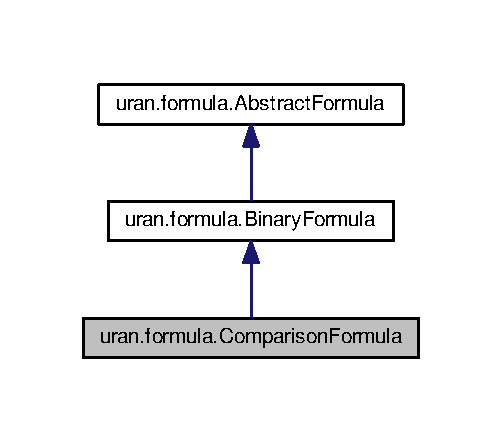
\includegraphics[width=241pt]{classuran_1_1formula_1_1_comparison_formula__inherit__graph}
\end{center}
\end{figure}


Collaboration diagram for uran.\+formula.\+Comparison\+Formula\+:
\nopagebreak
\begin{figure}[H]
\begin{center}
\leavevmode
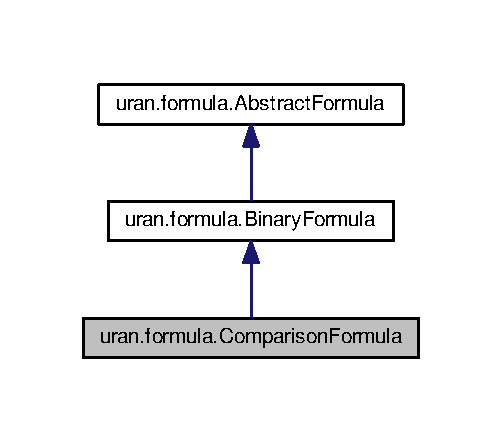
\includegraphics[width=241pt]{classuran_1_1formula_1_1_comparison_formula__coll__graph}
\end{center}
\end{figure}
\subsection*{Public Member Functions}
\begin{DoxyCompactItemize}
\item 
\hyperlink{classuran_1_1formula_1_1_comparison_formula_a89331d5d308bd81a95529e42105c8a63}{Comparison\+Formula} (\hyperlink{enumuran_1_1formula_1_1_connective}{Connective} op)
\item 
\hyperlink{classuran_1_1formula_1_1_comparison_formula_a941e912ef158f780fed63a0e5e41b429}{Comparison\+Formula} (\hyperlink{enumuran_1_1formula_1_1_connective}{Connective} op, \hyperlink{classuran_1_1formula_1_1_abstract_formula}{Abstract\+Formula} f1, \hyperlink{classuran_1_1formula_1_1_abstract_formula}{Abstract\+Formula} f2)
\item 
\hyperlink{classuran_1_1formula_1_1_binary_formula}{Binary\+Formula} \hyperlink{classuran_1_1formula_1_1_comparison_formula_a0fc31ab03fc655bcd247351b75ce369d}{merge} (Abstract\+Formula...\+formulas)
\end{DoxyCompactItemize}


\subsection{Detailed Description}


Definition at line 20 of file Comparison\+Formula.\+java.



\subsection{Constructor \& Destructor Documentation}
\hypertarget{classuran_1_1formula_1_1_comparison_formula_a89331d5d308bd81a95529e42105c8a63}{}\index{uran\+::formula\+::\+Comparison\+Formula@{uran\+::formula\+::\+Comparison\+Formula}!Comparison\+Formula@{Comparison\+Formula}}
\index{Comparison\+Formula@{Comparison\+Formula}!uran\+::formula\+::\+Comparison\+Formula@{uran\+::formula\+::\+Comparison\+Formula}}
\subsubsection[{Comparison\+Formula}]{\setlength{\rightskip}{0pt plus 5cm}uran.\+formula.\+Comparison\+Formula.\+Comparison\+Formula (
\begin{DoxyParamCaption}
\item[{{\bf Connective}}]{op}
\end{DoxyParamCaption}
)\hspace{0.3cm}{\ttfamily [inline]}}\label{classuran_1_1formula_1_1_comparison_formula_a89331d5d308bd81a95529e42105c8a63}


Definition at line 22 of file Comparison\+Formula.\+java.

\hypertarget{classuran_1_1formula_1_1_comparison_formula_a941e912ef158f780fed63a0e5e41b429}{}\index{uran\+::formula\+::\+Comparison\+Formula@{uran\+::formula\+::\+Comparison\+Formula}!Comparison\+Formula@{Comparison\+Formula}}
\index{Comparison\+Formula@{Comparison\+Formula}!uran\+::formula\+::\+Comparison\+Formula@{uran\+::formula\+::\+Comparison\+Formula}}
\subsubsection[{Comparison\+Formula}]{\setlength{\rightskip}{0pt plus 5cm}uran.\+formula.\+Comparison\+Formula.\+Comparison\+Formula (
\begin{DoxyParamCaption}
\item[{{\bf Connective}}]{op, }
\item[{{\bf Abstract\+Formula}}]{f1, }
\item[{{\bf Abstract\+Formula}}]{f2}
\end{DoxyParamCaption}
)\hspace{0.3cm}{\ttfamily [inline]}}\label{classuran_1_1formula_1_1_comparison_formula_a941e912ef158f780fed63a0e5e41b429}


Definition at line 24 of file Comparison\+Formula.\+java.



\subsection{Member Function Documentation}
\hypertarget{classuran_1_1formula_1_1_comparison_formula_a0fc31ab03fc655bcd247351b75ce369d}{}\index{uran\+::formula\+::\+Comparison\+Formula@{uran\+::formula\+::\+Comparison\+Formula}!merge@{merge}}
\index{merge@{merge}!uran\+::formula\+::\+Comparison\+Formula@{uran\+::formula\+::\+Comparison\+Formula}}
\subsubsection[{merge}]{\setlength{\rightskip}{0pt plus 5cm}{\bf Binary\+Formula} uran.\+formula.\+Comparison\+Formula.\+merge (
\begin{DoxyParamCaption}
\item[{Abstract\+Formula...}]{formulas}
\end{DoxyParamCaption}
)\hspace{0.3cm}{\ttfamily [inline]}}\label{classuran_1_1formula_1_1_comparison_formula_a0fc31ab03fc655bcd247351b75ce369d}


Definition at line 41 of file Comparison\+Formula.\+java.



The documentation for this class was generated from the following file\+:\begin{DoxyCompactItemize}
\item 
/home/haowu/uran/src/uran/formula/\hyperlink{_comparison_formula_8java}{Comparison\+Formula.\+java}\end{DoxyCompactItemize}

\hypertarget{enumuran_1_1formula_1_1_connective}{}\section{uran.\+formula.\+Connective Enum Reference}
\label{enumuran_1_1formula_1_1_connective}\index{uran.\+formula.\+Connective@{uran.\+formula.\+Connective}}
\subsection*{Public Attributes}
\begin{DoxyCompactItemize}
\item 
\hyperlink{enumuran_1_1formula_1_1_connective_a90aafb9dc47b7700e3717c06f4c568c2}{to\+String}
\end{DoxyCompactItemize}


\subsection{Detailed Description}


Definition at line 16 of file Connective.\+java.



\subsection{Member Data Documentation}
\hypertarget{enumuran_1_1formula_1_1_connective_a90aafb9dc47b7700e3717c06f4c568c2}{}\index{uran\+::formula\+::\+Connective@{uran\+::formula\+::\+Connective}!to\+String@{to\+String}}
\index{to\+String@{to\+String}!uran\+::formula\+::\+Connective@{uran\+::formula\+::\+Connective}}
\subsubsection[{to\+String}]{\setlength{\rightskip}{0pt plus 5cm}uran.\+formula.\+Connective.\+to\+String}\label{enumuran_1_1formula_1_1_connective_a90aafb9dc47b7700e3717c06f4c568c2}
{\bfseries Initial value\+:}
\begin{DoxyCode}
=()\{\textcolor{keywordflow}{return} \textcolor{stringliteral}{"and"};\}\},
    OR \{\textcolor{keyword}{public} String \hyperlink{enumuran_1_1formula_1_1_connective_a90aafb9dc47b7700e3717c06f4c568c2}{toString}()\{\textcolor{keywordflow}{return} \textcolor{stringliteral}{"or"};\}\},
    XOR \{\textcolor{keyword}{public} String \hyperlink{enumuran_1_1formula_1_1_connective_a90aafb9dc47b7700e3717c06f4c568c2}{toString}()\{\textcolor{keywordflow}{return} \textcolor{stringliteral}{"xor"};\}\},
    IMPLIES \{\textcolor{keyword}{public} String \hyperlink{enumuran_1_1formula_1_1_connective_a90aafb9dc47b7700e3717c06f4c568c2}{toString}()\{\textcolor{keywordflow}{return} \textcolor{stringliteral}{"=>"};\}\},
    NOT \{\textcolor{keyword}{public} String \hyperlink{enumuran_1_1formula_1_1_connective_a90aafb9dc47b7700e3717c06f4c568c2}{toString}()\{\textcolor{keywordflow}{return} \textcolor{stringliteral}{"not"};\}\},
    IFF \{\textcolor{keyword}{public} String \hyperlink{enumuran_1_1formula_1_1_connective_a90aafb9dc47b7700e3717c06f4c568c2}{toString}()\{\textcolor{keywordflow}{return} \textcolor{stringliteral}{"<=>"};\}\},
    EQUAL\{\textcolor{keyword}{public} String \hyperlink{enumuran_1_1formula_1_1_connective_a90aafb9dc47b7700e3717c06f4c568c2}{toString}()\{\textcolor{keywordflow}{return} \textcolor{stringliteral}{"="};\}\},
    PLUS\{\textcolor{keyword}{public} String \hyperlink{enumuran_1_1formula_1_1_connective_a90aafb9dc47b7700e3717c06f4c568c2}{toString}()\{\textcolor{keywordflow}{return} \textcolor{stringliteral}{"+"};\}\},
    MINUS\{\textcolor{keyword}{public} String \hyperlink{enumuran_1_1formula_1_1_connective_a90aafb9dc47b7700e3717c06f4c568c2}{toString}()\{\textcolor{keywordflow}{return} \textcolor{stringliteral}{"-"};\}\},
    MUL\{\textcolor{keyword}{public} String \hyperlink{enumuran_1_1formula_1_1_connective_a90aafb9dc47b7700e3717c06f4c568c2}{toString}()\{\textcolor{keywordflow}{return} \textcolor{stringliteral}{"*"};\}\},
    DIV\{\textcolor{keyword}{public} String \hyperlink{enumuran_1_1formula_1_1_connective_a90aafb9dc47b7700e3717c06f4c568c2}{toString}()\{\textcolor{keywordflow}{return} \textcolor{stringliteral}{"div"};\}\},
    GREATER\{\textcolor{keyword}{public} String \hyperlink{enumuran_1_1formula_1_1_connective_a90aafb9dc47b7700e3717c06f4c568c2}{toString}()\{\textcolor{keywordflow}{return} \textcolor{stringliteral}{">"};\}\},
    LESS\{\textcolor{keyword}{public} String \hyperlink{enumuran_1_1formula_1_1_connective_a90aafb9dc47b7700e3717c06f4c568c2}{toString}()\{\textcolor{keywordflow}{return} \textcolor{stringliteral}{"<"};\}\},
    GEQ\{\textcolor{keyword}{public} String \hyperlink{enumuran_1_1formula_1_1_connective_a90aafb9dc47b7700e3717c06f4c568c2}{toString}()\{\textcolor{keywordflow}{return} \textcolor{stringliteral}{">="};\}\},    
    LEQ\{\textcolor{keyword}{public} String \hyperlink{enumuran_1_1formula_1_1_connective_a90aafb9dc47b7700e3717c06f4c568c2}{toString}()\{\textcolor{keywordflow}{return} \textcolor{stringliteral}{"<="};\}\}
\end{DoxyCode}


Definition at line 17 of file Connective.\+java.



The documentation for this enum was generated from the following file\+:\begin{DoxyCompactItemize}
\item 
/home/haowu/uran/src/uran/formula/\hyperlink{_connective_8java}{Connective.\+java}\end{DoxyCompactItemize}

\hypertarget{classuran_1_1formula_1_1_constant}{}\section{uran.\+formula.\+Constant Class Reference}
\label{classuran_1_1formula_1_1_constant}\index{uran.\+formula.\+Constant@{uran.\+formula.\+Constant}}


Inheritance diagram for uran.\+formula.\+Constant\+:
\nopagebreak
\begin{figure}[H]
\begin{center}
\leavevmode
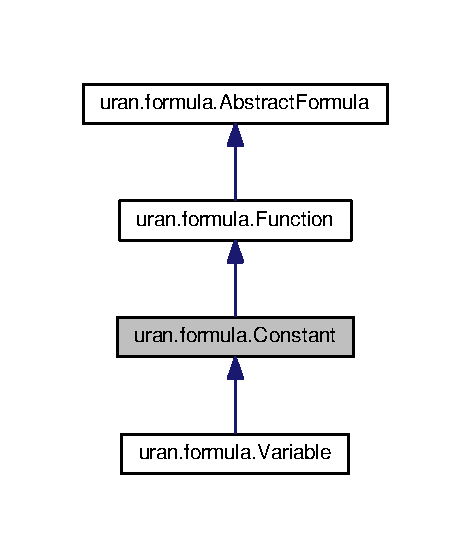
\includegraphics[width=226pt]{classuran_1_1formula_1_1_constant__inherit__graph}
\end{center}
\end{figure}


Collaboration diagram for uran.\+formula.\+Constant\+:
\nopagebreak
\begin{figure}[H]
\begin{center}
\leavevmode
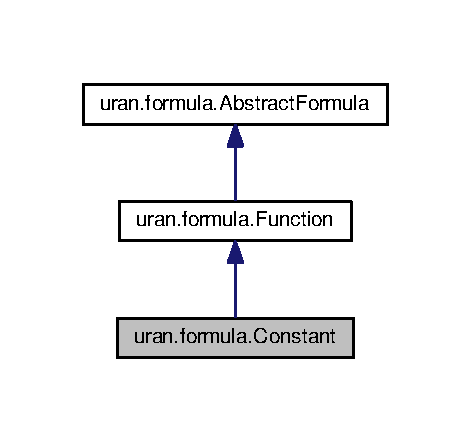
\includegraphics[width=226pt]{classuran_1_1formula_1_1_constant__coll__graph}
\end{center}
\end{figure}
\subsection*{Public Member Functions}
\begin{DoxyCompactItemize}
\item 
\hyperlink{classuran_1_1formula_1_1_constant_ac6f961836acdbc122a3b062c379ffc43}{Constant} (String name, \hyperlink{classuran_1_1formula_1_1type_1_1_type}{Type} type)
\item 
String \hyperlink{classuran_1_1formula_1_1_constant_a88de8c6bda20843b0755d001cc92bdee}{to\+S\+M\+T2} ()
\item 
String \hyperlink{classuran_1_1formula_1_1_constant_adde5eeda9f0345f6469e07ce924d9da8}{to\+String} ()
\item 
boolean \hyperlink{classuran_1_1formula_1_1_constant_a813dd0f4c306f21ec07be3e7e9f21ac7}{is\+Constant} ()
\end{DoxyCompactItemize}


\subsection{Detailed Description}


Definition at line 17 of file Constant.\+java.



\subsection{Constructor \& Destructor Documentation}
\hypertarget{classuran_1_1formula_1_1_constant_ac6f961836acdbc122a3b062c379ffc43}{}\index{uran\+::formula\+::\+Constant@{uran\+::formula\+::\+Constant}!Constant@{Constant}}
\index{Constant@{Constant}!uran\+::formula\+::\+Constant@{uran\+::formula\+::\+Constant}}
\subsubsection[{Constant}]{\setlength{\rightskip}{0pt plus 5cm}uran.\+formula.\+Constant.\+Constant (
\begin{DoxyParamCaption}
\item[{String}]{name, }
\item[{{\bf Type}}]{type}
\end{DoxyParamCaption}
)\hspace{0.3cm}{\ttfamily [inline]}}\label{classuran_1_1formula_1_1_constant_ac6f961836acdbc122a3b062c379ffc43}


Definition at line 18 of file Constant.\+java.



\subsection{Member Function Documentation}
\hypertarget{classuran_1_1formula_1_1_constant_a813dd0f4c306f21ec07be3e7e9f21ac7}{}\index{uran\+::formula\+::\+Constant@{uran\+::formula\+::\+Constant}!is\+Constant@{is\+Constant}}
\index{is\+Constant@{is\+Constant}!uran\+::formula\+::\+Constant@{uran\+::formula\+::\+Constant}}
\subsubsection[{is\+Constant}]{\setlength{\rightskip}{0pt plus 5cm}boolean uran.\+formula.\+Constant.\+is\+Constant (
\begin{DoxyParamCaption}
{}
\end{DoxyParamCaption}
)\hspace{0.3cm}{\ttfamily [inline]}}\label{classuran_1_1formula_1_1_constant_a813dd0f4c306f21ec07be3e7e9f21ac7}


Definition at line 30 of file Constant.\+java.

\hypertarget{classuran_1_1formula_1_1_constant_a88de8c6bda20843b0755d001cc92bdee}{}\index{uran\+::formula\+::\+Constant@{uran\+::formula\+::\+Constant}!to\+S\+M\+T2@{to\+S\+M\+T2}}
\index{to\+S\+M\+T2@{to\+S\+M\+T2}!uran\+::formula\+::\+Constant@{uran\+::formula\+::\+Constant}}
\subsubsection[{to\+S\+M\+T2}]{\setlength{\rightskip}{0pt plus 5cm}String uran.\+formula.\+Constant.\+to\+S\+M\+T2 (
\begin{DoxyParamCaption}
{}
\end{DoxyParamCaption}
)\hspace{0.3cm}{\ttfamily [inline]}}\label{classuran_1_1formula_1_1_constant_a88de8c6bda20843b0755d001cc92bdee}
apply to itself 

Definition at line 24 of file Constant.\+java.

\hypertarget{classuran_1_1formula_1_1_constant_adde5eeda9f0345f6469e07ce924d9da8}{}\index{uran\+::formula\+::\+Constant@{uran\+::formula\+::\+Constant}!to\+String@{to\+String}}
\index{to\+String@{to\+String}!uran\+::formula\+::\+Constant@{uran\+::formula\+::\+Constant}}
\subsubsection[{to\+String}]{\setlength{\rightskip}{0pt plus 5cm}String uran.\+formula.\+Constant.\+to\+String (
\begin{DoxyParamCaption}
{}
\end{DoxyParamCaption}
)\hspace{0.3cm}{\ttfamily [inline]}}\label{classuran_1_1formula_1_1_constant_adde5eeda9f0345f6469e07ce924d9da8}


Definition at line 27 of file Constant.\+java.



The documentation for this class was generated from the following file\+:\begin{DoxyCompactItemize}
\item 
/home/haowu/uran/src/uran/formula/\hyperlink{_constant_8java}{Constant.\+java}\end{DoxyCompactItemize}

\hypertarget{classuran_1_1formula_1_1_decls}{}\section{uran.\+formula.\+Decls Class Reference}
\label{classuran_1_1formula_1_1_decls}\index{uran.\+formula.\+Decls@{uran.\+formula.\+Decls}}


Inheritance diagram for uran.\+formula.\+Decls\+:
\nopagebreak
\begin{figure}[H]
\begin{center}
\leavevmode
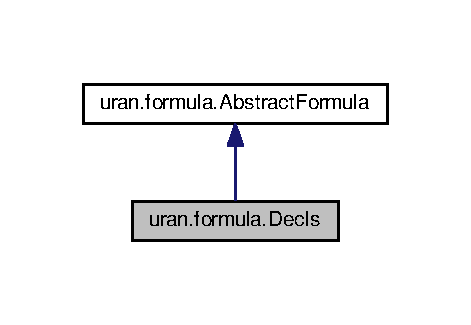
\includegraphics[width=226pt]{classuran_1_1formula_1_1_decls__inherit__graph}
\end{center}
\end{figure}


Collaboration diagram for uran.\+formula.\+Decls\+:
\nopagebreak
\begin{figure}[H]
\begin{center}
\leavevmode
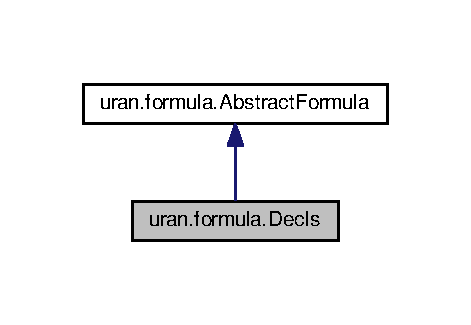
\includegraphics[width=226pt]{classuran_1_1formula_1_1_decls__coll__graph}
\end{center}
\end{figure}
\subsection*{Public Member Functions}
\begin{DoxyCompactItemize}
\item 
\hyperlink{classuran_1_1formula_1_1_decls_afb0b067c50f109bccd135179a834859d}{Decls} (Constant...\+v)
\item 
int \hyperlink{classuran_1_1formula_1_1_decls_a2011109f90bc8ffe0a2411a956b9d757}{size} ()
\item 
\hyperlink{classuran_1_1formula_1_1_constant}{Constant} \hyperlink{classuran_1_1formula_1_1_decls_af93470d252ebc0b03555ebce6a3bf5a3}{get} (int index)
\item 
\hyperlink{classuran_1_1formula_1_1_constant}{Constant}\mbox{[}$\,$\mbox{]} \hyperlink{classuran_1_1formula_1_1_decls_adf2d05c966db5338ff25d1bef6f995e2}{get} ()
\item 
String \hyperlink{classuran_1_1formula_1_1_decls_a6f2c79fc64944af8d53a036c8dd8a359}{to\+String} ()
\item 
String \hyperlink{classuran_1_1formula_1_1_decls_a66e6378a9e7d33ec467c46e594e66b31}{to\+S\+M\+T2} ()
\item 
void \hyperlink{classuran_1_1formula_1_1_decls_a18db9be61e2433115e9460980a7f732b}{accept} (\hyperlink{classuran_1_1formula_1_1visitor_1_1_abstract_visitor}{Abstract\+Visitor} visitor)
\end{DoxyCompactItemize}


\subsection{Detailed Description}


Definition at line 19 of file Decls.\+java.



\subsection{Constructor \& Destructor Documentation}
\hypertarget{classuran_1_1formula_1_1_decls_afb0b067c50f109bccd135179a834859d}{}\index{uran\+::formula\+::\+Decls@{uran\+::formula\+::\+Decls}!Decls@{Decls}}
\index{Decls@{Decls}!uran\+::formula\+::\+Decls@{uran\+::formula\+::\+Decls}}
\subsubsection[{Decls}]{\setlength{\rightskip}{0pt plus 5cm}uran.\+formula.\+Decls.\+Decls (
\begin{DoxyParamCaption}
\item[{Constant...}]{v}
\end{DoxyParamCaption}
)\hspace{0.3cm}{\ttfamily [inline]}}\label{classuran_1_1formula_1_1_decls_afb0b067c50f109bccd135179a834859d}


Definition at line 22 of file Decls.\+java.



\subsection{Member Function Documentation}
\hypertarget{classuran_1_1formula_1_1_decls_a18db9be61e2433115e9460980a7f732b}{}\index{uran\+::formula\+::\+Decls@{uran\+::formula\+::\+Decls}!accept@{accept}}
\index{accept@{accept}!uran\+::formula\+::\+Decls@{uran\+::formula\+::\+Decls}}
\subsubsection[{accept}]{\setlength{\rightskip}{0pt plus 5cm}void uran.\+formula.\+Decls.\+accept (
\begin{DoxyParamCaption}
\item[{{\bf Abstract\+Visitor}}]{visitor}
\end{DoxyParamCaption}
)\hspace{0.3cm}{\ttfamily [inline]}}\label{classuran_1_1formula_1_1_decls_a18db9be61e2433115e9460980a7f732b}


Definition at line 58 of file Decls.\+java.

\hypertarget{classuran_1_1formula_1_1_decls_af93470d252ebc0b03555ebce6a3bf5a3}{}\index{uran\+::formula\+::\+Decls@{uran\+::formula\+::\+Decls}!get@{get}}
\index{get@{get}!uran\+::formula\+::\+Decls@{uran\+::formula\+::\+Decls}}
\subsubsection[{get}]{\setlength{\rightskip}{0pt plus 5cm}{\bf Constant} uran.\+formula.\+Decls.\+get (
\begin{DoxyParamCaption}
\item[{int}]{index}
\end{DoxyParamCaption}
)\hspace{0.3cm}{\ttfamily [inline]}}\label{classuran_1_1formula_1_1_decls_af93470d252ebc0b03555ebce6a3bf5a3}


Definition at line 33 of file Decls.\+java.

\hypertarget{classuran_1_1formula_1_1_decls_adf2d05c966db5338ff25d1bef6f995e2}{}\index{uran\+::formula\+::\+Decls@{uran\+::formula\+::\+Decls}!get@{get}}
\index{get@{get}!uran\+::formula\+::\+Decls@{uran\+::formula\+::\+Decls}}
\subsubsection[{get}]{\setlength{\rightskip}{0pt plus 5cm}{\bf Constant} \mbox{[}$\,$\mbox{]} uran.\+formula.\+Decls.\+get (
\begin{DoxyParamCaption}
{}
\end{DoxyParamCaption}
)\hspace{0.3cm}{\ttfamily [inline]}}\label{classuran_1_1formula_1_1_decls_adf2d05c966db5338ff25d1bef6f995e2}


Definition at line 38 of file Decls.\+java.

\hypertarget{classuran_1_1formula_1_1_decls_a2011109f90bc8ffe0a2411a956b9d757}{}\index{uran\+::formula\+::\+Decls@{uran\+::formula\+::\+Decls}!size@{size}}
\index{size@{size}!uran\+::formula\+::\+Decls@{uran\+::formula\+::\+Decls}}
\subsubsection[{size}]{\setlength{\rightskip}{0pt plus 5cm}int uran.\+formula.\+Decls.\+size (
\begin{DoxyParamCaption}
{}
\end{DoxyParamCaption}
)\hspace{0.3cm}{\ttfamily [inline]}}\label{classuran_1_1formula_1_1_decls_a2011109f90bc8ffe0a2411a956b9d757}


Definition at line 32 of file Decls.\+java.

\hypertarget{classuran_1_1formula_1_1_decls_a66e6378a9e7d33ec467c46e594e66b31}{}\index{uran\+::formula\+::\+Decls@{uran\+::formula\+::\+Decls}!to\+S\+M\+T2@{to\+S\+M\+T2}}
\index{to\+S\+M\+T2@{to\+S\+M\+T2}!uran\+::formula\+::\+Decls@{uran\+::formula\+::\+Decls}}
\subsubsection[{to\+S\+M\+T2}]{\setlength{\rightskip}{0pt plus 5cm}String uran.\+formula.\+Decls.\+to\+S\+M\+T2 (
\begin{DoxyParamCaption}
{}
\end{DoxyParamCaption}
)\hspace{0.3cm}{\ttfamily [inline]}}\label{classuran_1_1formula_1_1_decls_a66e6378a9e7d33ec467c46e594e66b31}


Definition at line 53 of file Decls.\+java.

\hypertarget{classuran_1_1formula_1_1_decls_a6f2c79fc64944af8d53a036c8dd8a359}{}\index{uran\+::formula\+::\+Decls@{uran\+::formula\+::\+Decls}!to\+String@{to\+String}}
\index{to\+String@{to\+String}!uran\+::formula\+::\+Decls@{uran\+::formula\+::\+Decls}}
\subsubsection[{to\+String}]{\setlength{\rightskip}{0pt plus 5cm}String uran.\+formula.\+Decls.\+to\+String (
\begin{DoxyParamCaption}
{}
\end{DoxyParamCaption}
)\hspace{0.3cm}{\ttfamily [inline]}}\label{classuran_1_1formula_1_1_decls_a6f2c79fc64944af8d53a036c8dd8a359}


Definition at line 41 of file Decls.\+java.



The documentation for this class was generated from the following file\+:\begin{DoxyCompactItemize}
\item 
/home/haowu/uran/src/uran/formula/\hyperlink{_decls_8java}{Decls.\+java}\end{DoxyCompactItemize}

\hypertarget{classuran_1_1err_1_1_duplicated_declaration}{}\section{uran.\+err.\+Duplicated\+Declaration Class Reference}
\label{classuran_1_1err_1_1_duplicated_declaration}\index{uran.\+err.\+Duplicated\+Declaration@{uran.\+err.\+Duplicated\+Declaration}}


Inheritance diagram for uran.\+err.\+Duplicated\+Declaration\+:
\nopagebreak
\begin{figure}[H]
\begin{center}
\leavevmode
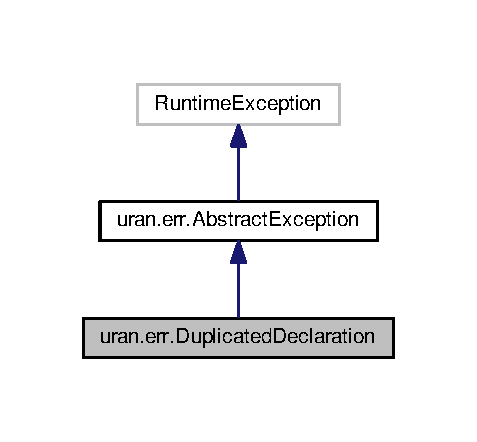
\includegraphics[width=229pt]{classuran_1_1err_1_1_duplicated_declaration__inherit__graph}
\end{center}
\end{figure}


Collaboration diagram for uran.\+err.\+Duplicated\+Declaration\+:
\nopagebreak
\begin{figure}[H]
\begin{center}
\leavevmode
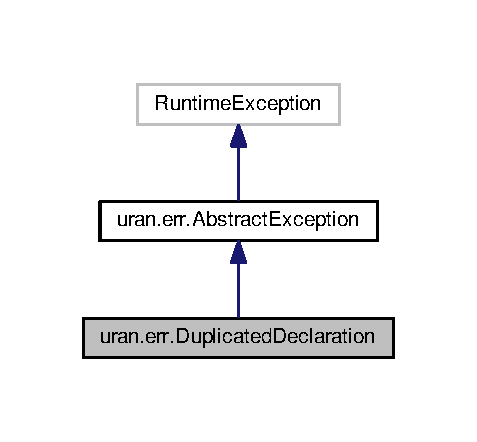
\includegraphics[width=229pt]{classuran_1_1err_1_1_duplicated_declaration__coll__graph}
\end{center}
\end{figure}
\subsection*{Public Member Functions}
\begin{DoxyCompactItemize}
\item 
\hyperlink{classuran_1_1err_1_1_duplicated_declaration_a3910648c38e3789c39fd9fa2d79c829a}{Duplicated\+Declaration} ()
\item 
\hyperlink{classuran_1_1err_1_1_duplicated_declaration_a46697afaaeb2f3b2d3303073e9caab39}{Duplicated\+Declaration} (String msg)
\end{DoxyCompactItemize}
\subsection*{Additional Inherited Members}


\subsection{Detailed Description}


Definition at line 16 of file Duplicated\+Declaration.\+java.



\subsection{Constructor \& Destructor Documentation}
\hypertarget{classuran_1_1err_1_1_duplicated_declaration_a3910648c38e3789c39fd9fa2d79c829a}{}\index{uran\+::err\+::\+Duplicated\+Declaration@{uran\+::err\+::\+Duplicated\+Declaration}!Duplicated\+Declaration@{Duplicated\+Declaration}}
\index{Duplicated\+Declaration@{Duplicated\+Declaration}!uran\+::err\+::\+Duplicated\+Declaration@{uran\+::err\+::\+Duplicated\+Declaration}}
\subsubsection[{Duplicated\+Declaration}]{\setlength{\rightskip}{0pt plus 5cm}uran.\+err.\+Duplicated\+Declaration.\+Duplicated\+Declaration (
\begin{DoxyParamCaption}
{}
\end{DoxyParamCaption}
)\hspace{0.3cm}{\ttfamily [inline]}}\label{classuran_1_1err_1_1_duplicated_declaration_a3910648c38e3789c39fd9fa2d79c829a}


Definition at line 18 of file Duplicated\+Declaration.\+java.

\hypertarget{classuran_1_1err_1_1_duplicated_declaration_a46697afaaeb2f3b2d3303073e9caab39}{}\index{uran\+::err\+::\+Duplicated\+Declaration@{uran\+::err\+::\+Duplicated\+Declaration}!Duplicated\+Declaration@{Duplicated\+Declaration}}
\index{Duplicated\+Declaration@{Duplicated\+Declaration}!uran\+::err\+::\+Duplicated\+Declaration@{uran\+::err\+::\+Duplicated\+Declaration}}
\subsubsection[{Duplicated\+Declaration}]{\setlength{\rightskip}{0pt plus 5cm}uran.\+err.\+Duplicated\+Declaration.\+Duplicated\+Declaration (
\begin{DoxyParamCaption}
\item[{String}]{msg}
\end{DoxyParamCaption}
)\hspace{0.3cm}{\ttfamily [inline]}}\label{classuran_1_1err_1_1_duplicated_declaration_a46697afaaeb2f3b2d3303073e9caab39}


Definition at line 23 of file Duplicated\+Declaration.\+java.



The documentation for this class was generated from the following file\+:\begin{DoxyCompactItemize}
\item 
/home/haowu/uran/src/uran/err/\hyperlink{_duplicated_declaration_8java}{Duplicated\+Declaration.\+java}\end{DoxyCompactItemize}

\hypertarget{classuran_1_1formula_1_1_eq_formula}{}\section{uran.\+formula.\+Eq\+Formula Class Reference}
\label{classuran_1_1formula_1_1_eq_formula}\index{uran.\+formula.\+Eq\+Formula@{uran.\+formula.\+Eq\+Formula}}


Inheritance diagram for uran.\+formula.\+Eq\+Formula\+:
\nopagebreak
\begin{figure}[H]
\begin{center}
\leavevmode
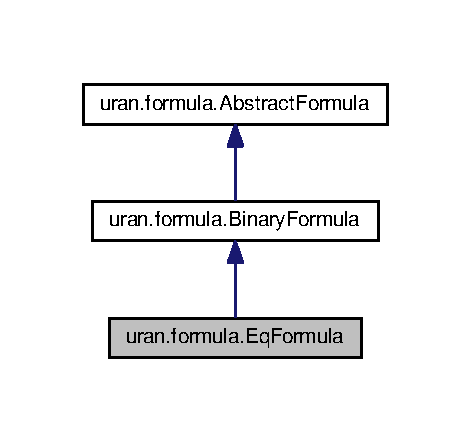
\includegraphics[width=226pt]{classuran_1_1formula_1_1_eq_formula__inherit__graph}
\end{center}
\end{figure}


Collaboration diagram for uran.\+formula.\+Eq\+Formula\+:
\nopagebreak
\begin{figure}[H]
\begin{center}
\leavevmode
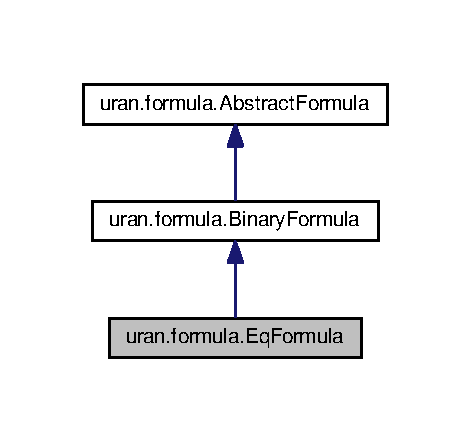
\includegraphics[width=226pt]{classuran_1_1formula_1_1_eq_formula__coll__graph}
\end{center}
\end{figure}
\subsection*{Public Member Functions}
\begin{DoxyCompactItemize}
\item 
\hyperlink{classuran_1_1formula_1_1_eq_formula_ad89285f320b8cad2040b744fac50059a}{Eq\+Formula} ()
\item 
\hyperlink{classuran_1_1formula_1_1_eq_formula_aa29c160f77006c11fa0f1efc109a3d61}{Eq\+Formula} (\hyperlink{classuran_1_1formula_1_1_abstract_formula}{Abstract\+Formula} f1, \hyperlink{classuran_1_1formula_1_1_abstract_formula}{Abstract\+Formula} f2)
\item 
\hyperlink{classuran_1_1formula_1_1_binary_formula}{Binary\+Formula} \hyperlink{classuran_1_1formula_1_1_eq_formula_a229ce93fa68be11e25b14f11d1378efd}{merge} (Abstract\+Formula...\+formulas)
\item 
boolean \hyperlink{classuran_1_1formula_1_1_eq_formula_addd48f076cedc4a0fec55879dc98eb16}{is\+Eq\+Formula} ()
\end{DoxyCompactItemize}


\subsection{Detailed Description}


Definition at line 19 of file Eq\+Formula.\+java.



\subsection{Constructor \& Destructor Documentation}
\hypertarget{classuran_1_1formula_1_1_eq_formula_ad89285f320b8cad2040b744fac50059a}{}\index{uran\+::formula\+::\+Eq\+Formula@{uran\+::formula\+::\+Eq\+Formula}!Eq\+Formula@{Eq\+Formula}}
\index{Eq\+Formula@{Eq\+Formula}!uran\+::formula\+::\+Eq\+Formula@{uran\+::formula\+::\+Eq\+Formula}}
\subsubsection[{Eq\+Formula}]{\setlength{\rightskip}{0pt plus 5cm}uran.\+formula.\+Eq\+Formula.\+Eq\+Formula (
\begin{DoxyParamCaption}
{}
\end{DoxyParamCaption}
)\hspace{0.3cm}{\ttfamily [inline]}}\label{classuran_1_1formula_1_1_eq_formula_ad89285f320b8cad2040b744fac50059a}


Definition at line 21 of file Eq\+Formula.\+java.

\hypertarget{classuran_1_1formula_1_1_eq_formula_aa29c160f77006c11fa0f1efc109a3d61}{}\index{uran\+::formula\+::\+Eq\+Formula@{uran\+::formula\+::\+Eq\+Formula}!Eq\+Formula@{Eq\+Formula}}
\index{Eq\+Formula@{Eq\+Formula}!uran\+::formula\+::\+Eq\+Formula@{uran\+::formula\+::\+Eq\+Formula}}
\subsubsection[{Eq\+Formula}]{\setlength{\rightskip}{0pt plus 5cm}uran.\+formula.\+Eq\+Formula.\+Eq\+Formula (
\begin{DoxyParamCaption}
\item[{{\bf Abstract\+Formula}}]{f1, }
\item[{{\bf Abstract\+Formula}}]{f2}
\end{DoxyParamCaption}
)\hspace{0.3cm}{\ttfamily [inline]}}\label{classuran_1_1formula_1_1_eq_formula_aa29c160f77006c11fa0f1efc109a3d61}


Definition at line 23 of file Eq\+Formula.\+java.



\subsection{Member Function Documentation}
\hypertarget{classuran_1_1formula_1_1_eq_formula_addd48f076cedc4a0fec55879dc98eb16}{}\index{uran\+::formula\+::\+Eq\+Formula@{uran\+::formula\+::\+Eq\+Formula}!is\+Eq\+Formula@{is\+Eq\+Formula}}
\index{is\+Eq\+Formula@{is\+Eq\+Formula}!uran\+::formula\+::\+Eq\+Formula@{uran\+::formula\+::\+Eq\+Formula}}
\subsubsection[{is\+Eq\+Formula}]{\setlength{\rightskip}{0pt plus 5cm}boolean uran.\+formula.\+Eq\+Formula.\+is\+Eq\+Formula (
\begin{DoxyParamCaption}
{}
\end{DoxyParamCaption}
)\hspace{0.3cm}{\ttfamily [inline]}}\label{classuran_1_1formula_1_1_eq_formula_addd48f076cedc4a0fec55879dc98eb16}


Definition at line 56 of file Eq\+Formula.\+java.

\hypertarget{classuran_1_1formula_1_1_eq_formula_a229ce93fa68be11e25b14f11d1378efd}{}\index{uran\+::formula\+::\+Eq\+Formula@{uran\+::formula\+::\+Eq\+Formula}!merge@{merge}}
\index{merge@{merge}!uran\+::formula\+::\+Eq\+Formula@{uran\+::formula\+::\+Eq\+Formula}}
\subsubsection[{merge}]{\setlength{\rightskip}{0pt plus 5cm}{\bf Binary\+Formula} uran.\+formula.\+Eq\+Formula.\+merge (
\begin{DoxyParamCaption}
\item[{Abstract\+Formula...}]{formulas}
\end{DoxyParamCaption}
)\hspace{0.3cm}{\ttfamily [inline]}}\label{classuran_1_1formula_1_1_eq_formula_a229ce93fa68be11e25b14f11d1378efd}


Definition at line 28 of file Eq\+Formula.\+java.



The documentation for this class was generated from the following file\+:\begin{DoxyCompactItemize}
\item 
/home/haowu/uran/src/uran/formula/\hyperlink{_eq_formula_8java}{Eq\+Formula.\+java}\end{DoxyCompactItemize}

\hypertarget{classuran_1_1formula_1_1_formula_builder}{}\section{uran.\+formula.\+Formula\+Builder Class Reference}
\label{classuran_1_1formula_1_1_formula_builder}\index{uran.\+formula.\+Formula\+Builder@{uran.\+formula.\+Formula\+Builder}}
\subsection*{Static Public Member Functions}
\begin{DoxyCompactItemize}
\item 
static \hyperlink{classuran_1_1formula_1_1_abstract_formula}{Abstract\+Formula} \hyperlink{classuran_1_1formula_1_1_formula_builder_a80fc1724f6b5c5e9834568e59a4303d9}{some} (Abstract\+Formula...\+formulas)
\item 
static \hyperlink{classuran_1_1formula_1_1_abstract_formula}{Abstract\+Formula} \hyperlink{classuran_1_1formula_1_1_formula_builder_adb0d9418878555814f8234e8e6953b05}{one} (Abstract\+Formula...\+formulas)
\item 
static \hyperlink{classuran_1_1formula_1_1_abstract_formula}{Abstract\+Formula} \hyperlink{classuran_1_1formula_1_1_formula_builder_a0fd2c2839c928fd3bd2bab3232ff7cca}{all} (Abstract\+Formula...\+formulas)
\item 
static \hyperlink{classuran_1_1formula_1_1_abstract_formula}{Abstract\+Formula} \hyperlink{classuran_1_1formula_1_1_formula_builder_ac4c1b4e0b80ab6e32144d64887e0559c}{neg} (\hyperlink{classuran_1_1formula_1_1_abstract_formula}{Abstract\+Formula} formula)
\item 
static \hyperlink{classuran_1_1formula_1_1_abstract_formula}{Abstract\+Formula} \hyperlink{classuran_1_1formula_1_1_formula_builder_ad835c1c078e8d8cce065f8d4815e2f91}{neq} (\hyperlink{classuran_1_1formula_1_1_abstract_formula}{Abstract\+Formula} formula1, \hyperlink{classuran_1_1formula_1_1_abstract_formula}{Abstract\+Formula} formula2)
\item 
static \hyperlink{classuran_1_1formula_1_1_abstract_formula}{Abstract\+Formula} \hyperlink{classuran_1_1formula_1_1_formula_builder_af31ff9ba719cd2591cbd88a1231d6702}{sum} (int k, List$<$ \hyperlink{classuran_1_1formula_1_1_constant}{Constant} $>$ formulas)
\item 
static \hyperlink{classuran_1_1formula_1_1_abstract_formula}{Abstract\+Formula} \hyperlink{classuran_1_1formula_1_1_formula_builder_a11cfdf22fa5d102d58ee1a08f20c92c3}{sum} (int k, Abstract\+Formula...\+formulas)
\item 
static \hyperlink{classuran_1_1formula_1_1_abstract_formula}{Abstract\+Formula} \hyperlink{classuran_1_1formula_1_1_formula_builder_a7aef5ab233718ba61e4748d8f363e6a0}{none} (Abstract\+Formula...\+formulas)
\item 
static \hyperlink{classuran_1_1formula_1_1_abstract_formula}{Abstract\+Formula} \hyperlink{classuran_1_1formula_1_1_formula_builder_a8a3b18603167b29bea8e504ae55e8630}{exact} (int k, Abstract\+Formula...\+formulas)
\item 
static \hyperlink{classuran_1_1formula_1_1_abstract_formula}{Abstract\+Formula} \hyperlink{classuran_1_1formula_1_1_formula_builder_adbd35dbca246de85fbec3ce74147d2b0}{plus} (Abstract\+Formula...\+formulas)
\item 
static \hyperlink{classuran_1_1formula_1_1_abstract_formula}{Abstract\+Formula} \hyperlink{classuran_1_1formula_1_1_formula_builder_a6821d484c21c9b05b51b8e462c724daa}{plus} (List$<$ \hyperlink{classuran_1_1formula_1_1_constant}{Constant} $>$ formulas)
\item 
static \hyperlink{classuran_1_1formula_1_1_abstract_formula}{Abstract\+Formula} \hyperlink{classuran_1_1formula_1_1_formula_builder_a12b44f4c9e540a9b4e00bb65cc7b9f41}{above} (\hyperlink{classuran_1_1formula_1_1_abstract_formula}{Abstract\+Formula} f, int k, boolean inclusive)
\item 
static \hyperlink{classuran_1_1formula_1_1_abstract_formula}{Abstract\+Formula} \hyperlink{classuran_1_1formula_1_1_formula_builder_a7a7c2f674a038c43fd97dc23fa7000a1}{below} (\hyperlink{classuran_1_1formula_1_1_abstract_formula}{Abstract\+Formula} f, int k, boolean inclusive)
\item 
static \hyperlink{classuran_1_1formula_1_1_abstract_formula}{Abstract\+Formula} \hyperlink{classuran_1_1formula_1_1_formula_builder_a7aba28e616231a95339e0b2d7b0b6f0c}{negassign} (Abstract\+Formula...\+formulas)
\item 
static \hyperlink{classuran_1_1formula_1_1_abstract_formula}{Abstract\+Formula} \hyperlink{classuran_1_1formula_1_1_formula_builder_ad53585a072b50c7065bf0875a663a9fd}{range} (int k, int j, \hyperlink{classuran_1_1formula_1_1_function}{Function} f, boolean inclusive)
\end{DoxyCompactItemize}


\subsection{Detailed Description}


Definition at line 19 of file Formula\+Builder.\+java.



\subsection{Member Function Documentation}
\hypertarget{classuran_1_1formula_1_1_formula_builder_a12b44f4c9e540a9b4e00bb65cc7b9f41}{}\index{uran\+::formula\+::\+Formula\+Builder@{uran\+::formula\+::\+Formula\+Builder}!above@{above}}
\index{above@{above}!uran\+::formula\+::\+Formula\+Builder@{uran\+::formula\+::\+Formula\+Builder}}
\subsubsection[{above}]{\setlength{\rightskip}{0pt plus 5cm}static {\bf Abstract\+Formula} uran.\+formula.\+Formula\+Builder.\+above (
\begin{DoxyParamCaption}
\item[{{\bf Abstract\+Formula}}]{f, }
\item[{int}]{k, }
\item[{boolean}]{inclusive}
\end{DoxyParamCaption}
)\hspace{0.3cm}{\ttfamily [inline]}, {\ttfamily [static]}}\label{classuran_1_1formula_1_1_formula_builder_a12b44f4c9e540a9b4e00bb65cc7b9f41}


Definition at line 70 of file Formula\+Builder.\+java.

\hypertarget{classuran_1_1formula_1_1_formula_builder_a0fd2c2839c928fd3bd2bab3232ff7cca}{}\index{uran\+::formula\+::\+Formula\+Builder@{uran\+::formula\+::\+Formula\+Builder}!all@{all}}
\index{all@{all}!uran\+::formula\+::\+Formula\+Builder@{uran\+::formula\+::\+Formula\+Builder}}
\subsubsection[{all}]{\setlength{\rightskip}{0pt plus 5cm}static {\bf Abstract\+Formula} uran.\+formula.\+Formula\+Builder.\+all (
\begin{DoxyParamCaption}
\item[{Abstract\+Formula...}]{formulas}
\end{DoxyParamCaption}
)\hspace{0.3cm}{\ttfamily [inline]}, {\ttfamily [static]}}\label{classuran_1_1formula_1_1_formula_builder_a0fd2c2839c928fd3bd2bab3232ff7cca}


Definition at line 29 of file Formula\+Builder.\+java.

\hypertarget{classuran_1_1formula_1_1_formula_builder_a7a7c2f674a038c43fd97dc23fa7000a1}{}\index{uran\+::formula\+::\+Formula\+Builder@{uran\+::formula\+::\+Formula\+Builder}!below@{below}}
\index{below@{below}!uran\+::formula\+::\+Formula\+Builder@{uran\+::formula\+::\+Formula\+Builder}}
\subsubsection[{below}]{\setlength{\rightskip}{0pt plus 5cm}static {\bf Abstract\+Formula} uran.\+formula.\+Formula\+Builder.\+below (
\begin{DoxyParamCaption}
\item[{{\bf Abstract\+Formula}}]{f, }
\item[{int}]{k, }
\item[{boolean}]{inclusive}
\end{DoxyParamCaption}
)\hspace{0.3cm}{\ttfamily [inline]}, {\ttfamily [static]}}\label{classuran_1_1formula_1_1_formula_builder_a7a7c2f674a038c43fd97dc23fa7000a1}


Definition at line 78 of file Formula\+Builder.\+java.

\hypertarget{classuran_1_1formula_1_1_formula_builder_a8a3b18603167b29bea8e504ae55e8630}{}\index{uran\+::formula\+::\+Formula\+Builder@{uran\+::formula\+::\+Formula\+Builder}!exact@{exact}}
\index{exact@{exact}!uran\+::formula\+::\+Formula\+Builder@{uran\+::formula\+::\+Formula\+Builder}}
\subsubsection[{exact}]{\setlength{\rightskip}{0pt plus 5cm}static {\bf Abstract\+Formula} uran.\+formula.\+Formula\+Builder.\+exact (
\begin{DoxyParamCaption}
\item[{int}]{k, }
\item[{Abstract\+Formula...}]{formulas}
\end{DoxyParamCaption}
)\hspace{0.3cm}{\ttfamily [inline]}, {\ttfamily [static]}}\label{classuran_1_1formula_1_1_formula_builder_a8a3b18603167b29bea8e504ae55e8630}


Definition at line 58 of file Formula\+Builder.\+java.

\hypertarget{classuran_1_1formula_1_1_formula_builder_ac4c1b4e0b80ab6e32144d64887e0559c}{}\index{uran\+::formula\+::\+Formula\+Builder@{uran\+::formula\+::\+Formula\+Builder}!neg@{neg}}
\index{neg@{neg}!uran\+::formula\+::\+Formula\+Builder@{uran\+::formula\+::\+Formula\+Builder}}
\subsubsection[{neg}]{\setlength{\rightskip}{0pt plus 5cm}static {\bf Abstract\+Formula} uran.\+formula.\+Formula\+Builder.\+neg (
\begin{DoxyParamCaption}
\item[{{\bf Abstract\+Formula}}]{formula}
\end{DoxyParamCaption}
)\hspace{0.3cm}{\ttfamily [inline]}, {\ttfamily [static]}}\label{classuran_1_1formula_1_1_formula_builder_ac4c1b4e0b80ab6e32144d64887e0559c}


Definition at line 33 of file Formula\+Builder.\+java.

\hypertarget{classuran_1_1formula_1_1_formula_builder_a7aba28e616231a95339e0b2d7b0b6f0c}{}\index{uran\+::formula\+::\+Formula\+Builder@{uran\+::formula\+::\+Formula\+Builder}!negassign@{negassign}}
\index{negassign@{negassign}!uran\+::formula\+::\+Formula\+Builder@{uran\+::formula\+::\+Formula\+Builder}}
\subsubsection[{negassign}]{\setlength{\rightskip}{0pt plus 5cm}static {\bf Abstract\+Formula} uran.\+formula.\+Formula\+Builder.\+negassign (
\begin{DoxyParamCaption}
\item[{Abstract\+Formula...}]{formulas}
\end{DoxyParamCaption}
)\hspace{0.3cm}{\ttfamily [inline]}, {\ttfamily [static]}}\label{classuran_1_1formula_1_1_formula_builder_a7aba28e616231a95339e0b2d7b0b6f0c}


Definition at line 86 of file Formula\+Builder.\+java.

\hypertarget{classuran_1_1formula_1_1_formula_builder_ad835c1c078e8d8cce065f8d4815e2f91}{}\index{uran\+::formula\+::\+Formula\+Builder@{uran\+::formula\+::\+Formula\+Builder}!neq@{neq}}
\index{neq@{neq}!uran\+::formula\+::\+Formula\+Builder@{uran\+::formula\+::\+Formula\+Builder}}
\subsubsection[{neq}]{\setlength{\rightskip}{0pt plus 5cm}static {\bf Abstract\+Formula} uran.\+formula.\+Formula\+Builder.\+neq (
\begin{DoxyParamCaption}
\item[{{\bf Abstract\+Formula}}]{formula1, }
\item[{{\bf Abstract\+Formula}}]{formula2}
\end{DoxyParamCaption}
)\hspace{0.3cm}{\ttfamily [inline]}, {\ttfamily [static]}}\label{classuran_1_1formula_1_1_formula_builder_ad835c1c078e8d8cce065f8d4815e2f91}


Definition at line 37 of file Formula\+Builder.\+java.

\hypertarget{classuran_1_1formula_1_1_formula_builder_a7aef5ab233718ba61e4748d8f363e6a0}{}\index{uran\+::formula\+::\+Formula\+Builder@{uran\+::formula\+::\+Formula\+Builder}!none@{none}}
\index{none@{none}!uran\+::formula\+::\+Formula\+Builder@{uran\+::formula\+::\+Formula\+Builder}}
\subsubsection[{none}]{\setlength{\rightskip}{0pt plus 5cm}static {\bf Abstract\+Formula} uran.\+formula.\+Formula\+Builder.\+none (
\begin{DoxyParamCaption}
\item[{Abstract\+Formula...}]{formulas}
\end{DoxyParamCaption}
)\hspace{0.3cm}{\ttfamily [inline]}, {\ttfamily [static]}}\label{classuran_1_1formula_1_1_formula_builder_a7aef5ab233718ba61e4748d8f363e6a0}


Definition at line 54 of file Formula\+Builder.\+java.

\hypertarget{classuran_1_1formula_1_1_formula_builder_adb0d9418878555814f8234e8e6953b05}{}\index{uran\+::formula\+::\+Formula\+Builder@{uran\+::formula\+::\+Formula\+Builder}!one@{one}}
\index{one@{one}!uran\+::formula\+::\+Formula\+Builder@{uran\+::formula\+::\+Formula\+Builder}}
\subsubsection[{one}]{\setlength{\rightskip}{0pt plus 5cm}static {\bf Abstract\+Formula} uran.\+formula.\+Formula\+Builder.\+one (
\begin{DoxyParamCaption}
\item[{Abstract\+Formula...}]{formulas}
\end{DoxyParamCaption}
)\hspace{0.3cm}{\ttfamily [inline]}, {\ttfamily [static]}}\label{classuran_1_1formula_1_1_formula_builder_adb0d9418878555814f8234e8e6953b05}


Definition at line 25 of file Formula\+Builder.\+java.

\hypertarget{classuran_1_1formula_1_1_formula_builder_adbd35dbca246de85fbec3ce74147d2b0}{}\index{uran\+::formula\+::\+Formula\+Builder@{uran\+::formula\+::\+Formula\+Builder}!plus@{plus}}
\index{plus@{plus}!uran\+::formula\+::\+Formula\+Builder@{uran\+::formula\+::\+Formula\+Builder}}
\subsubsection[{plus}]{\setlength{\rightskip}{0pt plus 5cm}static {\bf Abstract\+Formula} uran.\+formula.\+Formula\+Builder.\+plus (
\begin{DoxyParamCaption}
\item[{Abstract\+Formula...}]{formulas}
\end{DoxyParamCaption}
)\hspace{0.3cm}{\ttfamily [inline]}, {\ttfamily [static]}}\label{classuran_1_1formula_1_1_formula_builder_adbd35dbca246de85fbec3ce74147d2b0}


Definition at line 62 of file Formula\+Builder.\+java.

\hypertarget{classuran_1_1formula_1_1_formula_builder_a6821d484c21c9b05b51b8e462c724daa}{}\index{uran\+::formula\+::\+Formula\+Builder@{uran\+::formula\+::\+Formula\+Builder}!plus@{plus}}
\index{plus@{plus}!uran\+::formula\+::\+Formula\+Builder@{uran\+::formula\+::\+Formula\+Builder}}
\subsubsection[{plus}]{\setlength{\rightskip}{0pt plus 5cm}static {\bf Abstract\+Formula} uran.\+formula.\+Formula\+Builder.\+plus (
\begin{DoxyParamCaption}
\item[{List$<$ {\bf Constant} $>$}]{formulas}
\end{DoxyParamCaption}
)\hspace{0.3cm}{\ttfamily [inline]}, {\ttfamily [static]}}\label{classuran_1_1formula_1_1_formula_builder_a6821d484c21c9b05b51b8e462c724daa}


Definition at line 66 of file Formula\+Builder.\+java.

\hypertarget{classuran_1_1formula_1_1_formula_builder_ad53585a072b50c7065bf0875a663a9fd}{}\index{uran\+::formula\+::\+Formula\+Builder@{uran\+::formula\+::\+Formula\+Builder}!range@{range}}
\index{range@{range}!uran\+::formula\+::\+Formula\+Builder@{uran\+::formula\+::\+Formula\+Builder}}
\subsubsection[{range}]{\setlength{\rightskip}{0pt plus 5cm}static {\bf Abstract\+Formula} uran.\+formula.\+Formula\+Builder.\+range (
\begin{DoxyParamCaption}
\item[{int}]{k, }
\item[{int}]{j, }
\item[{{\bf Function}}]{f, }
\item[{boolean}]{inclusive}
\end{DoxyParamCaption}
)\hspace{0.3cm}{\ttfamily [inline]}, {\ttfamily [static]}}\label{classuran_1_1formula_1_1_formula_builder_ad53585a072b50c7065bf0875a663a9fd}


Definition at line 90 of file Formula\+Builder.\+java.

\hypertarget{classuran_1_1formula_1_1_formula_builder_a80fc1724f6b5c5e9834568e59a4303d9}{}\index{uran\+::formula\+::\+Formula\+Builder@{uran\+::formula\+::\+Formula\+Builder}!some@{some}}
\index{some@{some}!uran\+::formula\+::\+Formula\+Builder@{uran\+::formula\+::\+Formula\+Builder}}
\subsubsection[{some}]{\setlength{\rightskip}{0pt plus 5cm}static {\bf Abstract\+Formula} uran.\+formula.\+Formula\+Builder.\+some (
\begin{DoxyParamCaption}
\item[{Abstract\+Formula...}]{formulas}
\end{DoxyParamCaption}
)\hspace{0.3cm}{\ttfamily [inline]}, {\ttfamily [static]}}\label{classuran_1_1formula_1_1_formula_builder_a80fc1724f6b5c5e9834568e59a4303d9}


Definition at line 21 of file Formula\+Builder.\+java.

\hypertarget{classuran_1_1formula_1_1_formula_builder_af31ff9ba719cd2591cbd88a1231d6702}{}\index{uran\+::formula\+::\+Formula\+Builder@{uran\+::formula\+::\+Formula\+Builder}!sum@{sum}}
\index{sum@{sum}!uran\+::formula\+::\+Formula\+Builder@{uran\+::formula\+::\+Formula\+Builder}}
\subsubsection[{sum}]{\setlength{\rightskip}{0pt plus 5cm}static {\bf Abstract\+Formula} uran.\+formula.\+Formula\+Builder.\+sum (
\begin{DoxyParamCaption}
\item[{int}]{k, }
\item[{List$<$ {\bf Constant} $>$}]{formulas}
\end{DoxyParamCaption}
)\hspace{0.3cm}{\ttfamily [inline]}, {\ttfamily [static]}}\label{classuran_1_1formula_1_1_formula_builder_af31ff9ba719cd2591cbd88a1231d6702}


Definition at line 41 of file Formula\+Builder.\+java.

\hypertarget{classuran_1_1formula_1_1_formula_builder_a11cfdf22fa5d102d58ee1a08f20c92c3}{}\index{uran\+::formula\+::\+Formula\+Builder@{uran\+::formula\+::\+Formula\+Builder}!sum@{sum}}
\index{sum@{sum}!uran\+::formula\+::\+Formula\+Builder@{uran\+::formula\+::\+Formula\+Builder}}
\subsubsection[{sum}]{\setlength{\rightskip}{0pt plus 5cm}static {\bf Abstract\+Formula} uran.\+formula.\+Formula\+Builder.\+sum (
\begin{DoxyParamCaption}
\item[{int}]{k, }
\item[{Abstract\+Formula...}]{formulas}
\end{DoxyParamCaption}
)\hspace{0.3cm}{\ttfamily [inline]}, {\ttfamily [static]}}\label{classuran_1_1formula_1_1_formula_builder_a11cfdf22fa5d102d58ee1a08f20c92c3}


Definition at line 45 of file Formula\+Builder.\+java.



The documentation for this class was generated from the following file\+:\begin{DoxyCompactItemize}
\item 
/home/haowu/uran/src/uran/formula/\hyperlink{_formula_builder_8java}{Formula\+Builder.\+java}\end{DoxyCompactItemize}

\hypertarget{classuran_1_1formula_1_1_function}{}\section{uran.\+formula.\+Function Class Reference}
\label{classuran_1_1formula_1_1_function}\index{uran.\+formula.\+Function@{uran.\+formula.\+Function}}


Inheritance diagram for uran.\+formula.\+Function\+:
\nopagebreak
\begin{figure}[H]
\begin{center}
\leavevmode
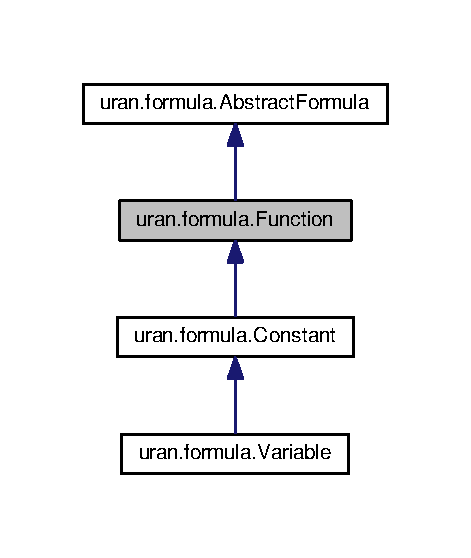
\includegraphics[width=226pt]{classuran_1_1formula_1_1_function__inherit__graph}
\end{center}
\end{figure}


Collaboration diagram for uran.\+formula.\+Function\+:
\nopagebreak
\begin{figure}[H]
\begin{center}
\leavevmode
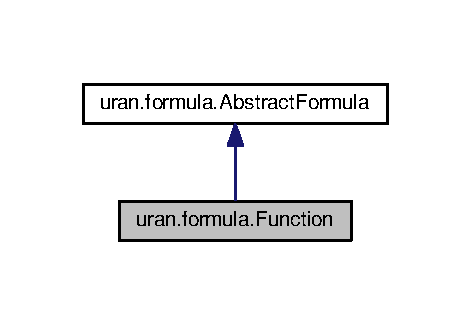
\includegraphics[width=226pt]{classuran_1_1formula_1_1_function__coll__graph}
\end{center}
\end{figure}
\subsection*{Public Member Functions}
\begin{DoxyCompactItemize}
\item 
\hyperlink{classuran_1_1formula_1_1_function_abab40ed046111627cab8d93b2780da11}{Function} (String n, Type...\+args)
\item 
\hyperlink{classuran_1_1formula_1_1_function_a8798b4f02f197741361be6596dc8f0f5}{Function} (\hyperlink{classuran_1_1formula_1_1_function}{Function} fun, Function...\+args)
\item 
int \hyperlink{classuran_1_1formula_1_1_function_a615e9611d49db496dcd3f74550a220cb}{arity} ()
\item 
String \hyperlink{classuran_1_1formula_1_1_function_acd825466dceed6c2d677895d9e156c27}{name} ()
\item 
\hyperlink{classuran_1_1formula_1_1type_1_1_type}{Type}\mbox{[}$\,$\mbox{]} \hyperlink{classuran_1_1formula_1_1_function_a48b08ecb2b2594ba31c63df397022e65}{get\+Args} ()
\item 
\hyperlink{classuran_1_1formula_1_1type_1_1_type}{Type} \hyperlink{classuran_1_1formula_1_1_function_ae44d77eca56a3d932e06715b8129ffd5}{get\+Args} (int index)
\item 
\hyperlink{classuran_1_1formula_1_1type_1_1_type}{Type} \hyperlink{classuran_1_1formula_1_1_function_a1284d625f45b675f2819578b1fea8fbe}{get\+Return\+Type} ()
\item 
boolean \hyperlink{classuran_1_1formula_1_1_function_a2cfe351a2f060618cbe571342b64e662}{is\+Constant} ()
\item 
boolean \hyperlink{classuran_1_1formula_1_1_function_ac06a993807911137fb8099bc0d3cc4e9}{is\+Function} ()
\item 
\hyperlink{classuran_1_1formula_1_1_function}{Function} \hyperlink{classuran_1_1formula_1_1_function_a39bab5b0fa754e4a24e2655f8003e32f}{apply} (Function...\+functions)
\item 
String \hyperlink{classuran_1_1formula_1_1_function_a118f8a1eaff250ed8ccc31603129bc0e}{to\+String} ()
\item 
String \hyperlink{classuran_1_1formula_1_1_function_a667a61d9acbae47f9de11ad8b354269c}{to\+S\+M\+T2} ()
\item 
String \hyperlink{classuran_1_1formula_1_1_function_af33e0ca53f19882649241248946a7f66}{to\+S\+M\+T2\+\_\+decl} ()
\item 
void \hyperlink{classuran_1_1formula_1_1_function_a36588b7e90d80b1a316c357b6099373b}{accept} (\hyperlink{classuran_1_1formula_1_1visitor_1_1_abstract_visitor}{Abstract\+Visitor} visitor)
\end{DoxyCompactItemize}


\subsection{Detailed Description}
Abstract syntax tree for function 

Definition at line 22 of file Function.\+java.



\subsection{Constructor \& Destructor Documentation}
\hypertarget{classuran_1_1formula_1_1_function_abab40ed046111627cab8d93b2780da11}{}\index{uran\+::formula\+::\+Function@{uran\+::formula\+::\+Function}!Function@{Function}}
\index{Function@{Function}!uran\+::formula\+::\+Function@{uran\+::formula\+::\+Function}}
\subsubsection[{Function}]{\setlength{\rightskip}{0pt plus 5cm}uran.\+formula.\+Function.\+Function (
\begin{DoxyParamCaption}
\item[{String}]{n, }
\item[{Type...}]{args}
\end{DoxyParamCaption}
)\hspace{0.3cm}{\ttfamily [inline]}}\label{classuran_1_1formula_1_1_function_abab40ed046111627cab8d93b2780da11}
Construct a function based on a list of argument type 

Definition at line 29 of file Function.\+java.

\hypertarget{classuran_1_1formula_1_1_function_a8798b4f02f197741361be6596dc8f0f5}{}\index{uran\+::formula\+::\+Function@{uran\+::formula\+::\+Function}!Function@{Function}}
\index{Function@{Function}!uran\+::formula\+::\+Function@{uran\+::formula\+::\+Function}}
\subsubsection[{Function}]{\setlength{\rightskip}{0pt plus 5cm}uran.\+formula.\+Function.\+Function (
\begin{DoxyParamCaption}
\item[{{\bf Function}}]{fun, }
\item[{Function...}]{args}
\end{DoxyParamCaption}
)\hspace{0.3cm}{\ttfamily [inline]}}\label{classuran_1_1formula_1_1_function_a8798b4f02f197741361be6596dc8f0f5}
Construct a function application 

Definition at line 43 of file Function.\+java.



\subsection{Member Function Documentation}
\hypertarget{classuran_1_1formula_1_1_function_a36588b7e90d80b1a316c357b6099373b}{}\index{uran\+::formula\+::\+Function@{uran\+::formula\+::\+Function}!accept@{accept}}
\index{accept@{accept}!uran\+::formula\+::\+Function@{uran\+::formula\+::\+Function}}
\subsubsection[{accept}]{\setlength{\rightskip}{0pt plus 5cm}void uran.\+formula.\+Function.\+accept (
\begin{DoxyParamCaption}
\item[{{\bf Abstract\+Visitor}}]{visitor}
\end{DoxyParamCaption}
)\hspace{0.3cm}{\ttfamily [inline]}}\label{classuran_1_1formula_1_1_function_a36588b7e90d80b1a316c357b6099373b}


Definition at line 141 of file Function.\+java.

\hypertarget{classuran_1_1formula_1_1_function_a39bab5b0fa754e4a24e2655f8003e32f}{}\index{uran\+::formula\+::\+Function@{uran\+::formula\+::\+Function}!apply@{apply}}
\index{apply@{apply}!uran\+::formula\+::\+Function@{uran\+::formula\+::\+Function}}
\subsubsection[{apply}]{\setlength{\rightskip}{0pt plus 5cm}{\bf Function} uran.\+formula.\+Function.\+apply (
\begin{DoxyParamCaption}
\item[{Function...}]{functions}
\end{DoxyParamCaption}
)\hspace{0.3cm}{\ttfamily [inline]}}\label{classuran_1_1formula_1_1_function_a39bab5b0fa754e4a24e2655f8003e32f}
Apply this function on a list of functions.


\begin{DoxyParams}{Parameters}
{\em functions} & list of functions to be applied on. \\
\hline
\end{DoxyParams}


Definition at line 92 of file Function.\+java.

\hypertarget{classuran_1_1formula_1_1_function_a615e9611d49db496dcd3f74550a220cb}{}\index{uran\+::formula\+::\+Function@{uran\+::formula\+::\+Function}!arity@{arity}}
\index{arity@{arity}!uran\+::formula\+::\+Function@{uran\+::formula\+::\+Function}}
\subsubsection[{arity}]{\setlength{\rightskip}{0pt plus 5cm}int uran.\+formula.\+Function.\+arity (
\begin{DoxyParamCaption}
{}
\end{DoxyParamCaption}
)\hspace{0.3cm}{\ttfamily [inline]}}\label{classuran_1_1formula_1_1_function_a615e9611d49db496dcd3f74550a220cb}
Return the arity of this function. 

Definition at line 51 of file Function.\+java.

\hypertarget{classuran_1_1formula_1_1_function_a48b08ecb2b2594ba31c63df397022e65}{}\index{uran\+::formula\+::\+Function@{uran\+::formula\+::\+Function}!get\+Args@{get\+Args}}
\index{get\+Args@{get\+Args}!uran\+::formula\+::\+Function@{uran\+::formula\+::\+Function}}
\subsubsection[{get\+Args}]{\setlength{\rightskip}{0pt plus 5cm}{\bf Type} \mbox{[}$\,$\mbox{]} uran.\+formula.\+Function.\+get\+Args (
\begin{DoxyParamCaption}
{}
\end{DoxyParamCaption}
)\hspace{0.3cm}{\ttfamily [inline]}}\label{classuran_1_1formula_1_1_function_a48b08ecb2b2594ba31c63df397022e65}
Return all arguments 

Definition at line 64 of file Function.\+java.

\hypertarget{classuran_1_1formula_1_1_function_ae44d77eca56a3d932e06715b8129ffd5}{}\index{uran\+::formula\+::\+Function@{uran\+::formula\+::\+Function}!get\+Args@{get\+Args}}
\index{get\+Args@{get\+Args}!uran\+::formula\+::\+Function@{uran\+::formula\+::\+Function}}
\subsubsection[{get\+Args}]{\setlength{\rightskip}{0pt plus 5cm}{\bf Type} uran.\+formula.\+Function.\+get\+Args (
\begin{DoxyParamCaption}
\item[{int}]{index}
\end{DoxyParamCaption}
)\hspace{0.3cm}{\ttfamily [inline]}}\label{classuran_1_1formula_1_1_function_ae44d77eca56a3d932e06715b8129ffd5}
Get a specific argument type. 

Definition at line 67 of file Function.\+java.

\hypertarget{classuran_1_1formula_1_1_function_a1284d625f45b675f2819578b1fea8fbe}{}\index{uran\+::formula\+::\+Function@{uran\+::formula\+::\+Function}!get\+Return\+Type@{get\+Return\+Type}}
\index{get\+Return\+Type@{get\+Return\+Type}!uran\+::formula\+::\+Function@{uran\+::formula\+::\+Function}}
\subsubsection[{get\+Return\+Type}]{\setlength{\rightskip}{0pt plus 5cm}{\bf Type} uran.\+formula.\+Function.\+get\+Return\+Type (
\begin{DoxyParamCaption}
{}
\end{DoxyParamCaption}
)\hspace{0.3cm}{\ttfamily [inline]}}\label{classuran_1_1formula_1_1_function_a1284d625f45b675f2819578b1fea8fbe}
Get the return type of this function. 

Definition at line 74 of file Function.\+java.

\hypertarget{classuran_1_1formula_1_1_function_a2cfe351a2f060618cbe571342b64e662}{}\index{uran\+::formula\+::\+Function@{uran\+::formula\+::\+Function}!is\+Constant@{is\+Constant}}
\index{is\+Constant@{is\+Constant}!uran\+::formula\+::\+Function@{uran\+::formula\+::\+Function}}
\subsubsection[{is\+Constant}]{\setlength{\rightskip}{0pt plus 5cm}boolean uran.\+formula.\+Function.\+is\+Constant (
\begin{DoxyParamCaption}
{}
\end{DoxyParamCaption}
)\hspace{0.3cm}{\ttfamily [inline]}}\label{classuran_1_1formula_1_1_function_a2cfe351a2f060618cbe571342b64e662}
A constant is that a function has 0 arity. 

Definition at line 80 of file Function.\+java.

\hypertarget{classuran_1_1formula_1_1_function_ac06a993807911137fb8099bc0d3cc4e9}{}\index{uran\+::formula\+::\+Function@{uran\+::formula\+::\+Function}!is\+Function@{is\+Function}}
\index{is\+Function@{is\+Function}!uran\+::formula\+::\+Function@{uran\+::formula\+::\+Function}}
\subsubsection[{is\+Function}]{\setlength{\rightskip}{0pt plus 5cm}boolean uran.\+formula.\+Function.\+is\+Function (
\begin{DoxyParamCaption}
{}
\end{DoxyParamCaption}
)\hspace{0.3cm}{\ttfamily [inline]}}\label{classuran_1_1formula_1_1_function_ac06a993807911137fb8099bc0d3cc4e9}
Returns true 

Definition at line 86 of file Function.\+java.

\hypertarget{classuran_1_1formula_1_1_function_acd825466dceed6c2d677895d9e156c27}{}\index{uran\+::formula\+::\+Function@{uran\+::formula\+::\+Function}!name@{name}}
\index{name@{name}!uran\+::formula\+::\+Function@{uran\+::formula\+::\+Function}}
\subsubsection[{name}]{\setlength{\rightskip}{0pt plus 5cm}String uran.\+formula.\+Function.\+name (
\begin{DoxyParamCaption}
{}
\end{DoxyParamCaption}
)\hspace{0.3cm}{\ttfamily [inline]}}\label{classuran_1_1formula_1_1_function_acd825466dceed6c2d677895d9e156c27}
Return the name of this function. 

Definition at line 57 of file Function.\+java.

\hypertarget{classuran_1_1formula_1_1_function_a667a61d9acbae47f9de11ad8b354269c}{}\index{uran\+::formula\+::\+Function@{uran\+::formula\+::\+Function}!to\+S\+M\+T2@{to\+S\+M\+T2}}
\index{to\+S\+M\+T2@{to\+S\+M\+T2}!uran\+::formula\+::\+Function@{uran\+::formula\+::\+Function}}
\subsubsection[{to\+S\+M\+T2}]{\setlength{\rightskip}{0pt plus 5cm}String uran.\+formula.\+Function.\+to\+S\+M\+T2 (
\begin{DoxyParamCaption}
{}
\end{DoxyParamCaption}
)\hspace{0.3cm}{\ttfamily [inline]}}\label{classuran_1_1formula_1_1_function_a667a61d9acbae47f9de11ad8b354269c}
This is for generating function application. N\+O\+T\+E\+: \hyperlink{classuran_1_1formula_1_1_function}{Function} declaration must be created 1st. 

Definition at line 119 of file Function.\+java.

\hypertarget{classuran_1_1formula_1_1_function_af33e0ca53f19882649241248946a7f66}{}\index{uran\+::formula\+::\+Function@{uran\+::formula\+::\+Function}!to\+S\+M\+T2\+\_\+decl@{to\+S\+M\+T2\+\_\+decl}}
\index{to\+S\+M\+T2\+\_\+decl@{to\+S\+M\+T2\+\_\+decl}!uran\+::formula\+::\+Function@{uran\+::formula\+::\+Function}}
\subsubsection[{to\+S\+M\+T2\+\_\+decl}]{\setlength{\rightskip}{0pt plus 5cm}String uran.\+formula.\+Function.\+to\+S\+M\+T2\+\_\+decl (
\begin{DoxyParamCaption}
{}
\end{DoxyParamCaption}
)\hspace{0.3cm}{\ttfamily [inline]}}\label{classuran_1_1formula_1_1_function_af33e0ca53f19882649241248946a7f66}
This is for generating declaration only. 

Definition at line 133 of file Function.\+java.

\hypertarget{classuran_1_1formula_1_1_function_a118f8a1eaff250ed8ccc31603129bc0e}{}\index{uran\+::formula\+::\+Function@{uran\+::formula\+::\+Function}!to\+String@{to\+String}}
\index{to\+String@{to\+String}!uran\+::formula\+::\+Function@{uran\+::formula\+::\+Function}}
\subsubsection[{to\+String}]{\setlength{\rightskip}{0pt plus 5cm}String uran.\+formula.\+Function.\+to\+String (
\begin{DoxyParamCaption}
{}
\end{DoxyParamCaption}
)\hspace{0.3cm}{\ttfamily [inline]}}\label{classuran_1_1formula_1_1_function_a118f8a1eaff250ed8ccc31603129bc0e}


Definition at line 105 of file Function.\+java.



The documentation for this class was generated from the following file\+:\begin{DoxyCompactItemize}
\item 
/home/haowu/uran/src/uran/formula/\hyperlink{_function_8java}{Function.\+java}\end{DoxyCompactItemize}

\hypertarget{classuran_1_1formula_1_1_function_factory}{}\section{uran.\+formula.\+Function\+Factory Class Reference}
\label{classuran_1_1formula_1_1_function_factory}\index{uran.\+formula.\+Function\+Factory@{uran.\+formula.\+Function\+Factory}}
\subsection*{Public Member Functions}
\begin{DoxyCompactItemize}
\item 
\hyperlink{classuran_1_1formula_1_1_function_factory_a93f76edeabe521e3b90377bb89cbb725}{Function\+Factory} ()
\item 
\hyperlink{classuran_1_1formula_1_1_function_factory_a38475ef8d6732b1f8f3fca34624791e1}{Function\+Factory} (int cap)
\item 
\hyperlink{classuran_1_1formula_1_1_function_factory_ab68f793821a4bc035673156bc7bc238e}{Function\+Factory} (int cap, float load)
\item 
\hyperlink{classuran_1_1formula_1_1_constant}{Constant} \hyperlink{classuran_1_1formula_1_1_function_factory_acaf3bd05dd854be14c7b7347a5cfe970}{create\+Constant} (String name, \hyperlink{classuran_1_1formula_1_1type_1_1_type}{Type} type)
\item 
\hyperlink{classuran_1_1formula_1_1_function}{Function} \hyperlink{classuran_1_1formula_1_1_function_factory_a49fb8c9efb968aa482706abbbf2deaa3}{create\+Function} (String name, Type...\+args)
\item 
\hyperlink{classuran_1_1formula_1_1_constant}{Constant} \hyperlink{classuran_1_1formula_1_1_function_factory_a3e2c6df5ad1b23b8b51d4775d1953a94}{con\+Lookup} (String name)
\item 
\hyperlink{classuran_1_1formula_1_1_function}{Function} \hyperlink{classuran_1_1formula_1_1_function_factory_a644cfc1803a1827e9ce03c26d6cf120d}{fun\+Lookup} (String name)
\item 
int \hyperlink{classuran_1_1formula_1_1_function_factory_ab939a92375538a729125986017109ccf}{size} ()
\item 
void \hyperlink{classuran_1_1formula_1_1_function_factory_abf9ab36c0b659982eb78945e595bfe98}{remove} (String name)
\item 
List$<$ \hyperlink{classuran_1_1formula_1_1_function}{Function} $>$ \hyperlink{classuran_1_1formula_1_1_function_factory_aec5c1bcbc24e6b9a9a292951ede73842}{get\+All\+Functions} ()
\item 
void \hyperlink{classuran_1_1formula_1_1_function_factory_a7e50687c28a06332cc6a5a51b06af4dd}{update\+Value} (String name, \hyperlink{classuran_1_1formula_1_1value_1_1_value}{Value} value)
\item 
\hyperlink{classuran_1_1formula_1_1value_1_1_value}{Value} \hyperlink{classuran_1_1formula_1_1_function_factory_a180524cdb52b336d9383eaebe1982f16}{get\+Value} (String name)
\item 
\hyperlink{classuran_1_1formula_1_1_neg_formula}{Neg\+Formula} \hyperlink{classuran_1_1formula_1_1_function_factory_a362a2c48f9aa26b479f2799d9ebd55ed}{neg\+Constants} ()
\item 
String \hyperlink{classuran_1_1formula_1_1_function_factory_abf221e7d663c9979ad9417984ce8d82f}{to\+String} ()
\end{DoxyCompactItemize}


\subsection{Detailed Description}
Factory for creating functions and constants, only these functions and constants created by factory are translated to S\+M\+T2. \begin{DoxyAuthor}{Author}
Hao Wu 
\end{DoxyAuthor}


Definition at line 39 of file Function\+Factory.\+java.



\subsection{Constructor \& Destructor Documentation}
\hypertarget{classuran_1_1formula_1_1_function_factory_a93f76edeabe521e3b90377bb89cbb725}{}\index{uran\+::formula\+::\+Function\+Factory@{uran\+::formula\+::\+Function\+Factory}!Function\+Factory@{Function\+Factory}}
\index{Function\+Factory@{Function\+Factory}!uran\+::formula\+::\+Function\+Factory@{uran\+::formula\+::\+Function\+Factory}}
\subsubsection[{Function\+Factory}]{\setlength{\rightskip}{0pt plus 5cm}uran.\+formula.\+Function\+Factory.\+Function\+Factory (
\begin{DoxyParamCaption}
{}
\end{DoxyParamCaption}
)\hspace{0.3cm}{\ttfamily [inline]}}\label{classuran_1_1formula_1_1_function_factory_a93f76edeabe521e3b90377bb89cbb725}
Create a factory with default ini capacity and load factor 

Definition at line 47 of file Function\+Factory.\+java.

\hypertarget{classuran_1_1formula_1_1_function_factory_a38475ef8d6732b1f8f3fca34624791e1}{}\index{uran\+::formula\+::\+Function\+Factory@{uran\+::formula\+::\+Function\+Factory}!Function\+Factory@{Function\+Factory}}
\index{Function\+Factory@{Function\+Factory}!uran\+::formula\+::\+Function\+Factory@{uran\+::formula\+::\+Function\+Factory}}
\subsubsection[{Function\+Factory}]{\setlength{\rightskip}{0pt plus 5cm}uran.\+formula.\+Function\+Factory.\+Function\+Factory (
\begin{DoxyParamCaption}
\item[{int}]{cap}
\end{DoxyParamCaption}
)\hspace{0.3cm}{\ttfamily [inline]}}\label{classuran_1_1formula_1_1_function_factory_a38475ef8d6732b1f8f3fca34624791e1}
Specify an ini capacity. 

Definition at line 53 of file Function\+Factory.\+java.

\hypertarget{classuran_1_1formula_1_1_function_factory_ab68f793821a4bc035673156bc7bc238e}{}\index{uran\+::formula\+::\+Function\+Factory@{uran\+::formula\+::\+Function\+Factory}!Function\+Factory@{Function\+Factory}}
\index{Function\+Factory@{Function\+Factory}!uran\+::formula\+::\+Function\+Factory@{uran\+::formula\+::\+Function\+Factory}}
\subsubsection[{Function\+Factory}]{\setlength{\rightskip}{0pt plus 5cm}uran.\+formula.\+Function\+Factory.\+Function\+Factory (
\begin{DoxyParamCaption}
\item[{int}]{cap, }
\item[{float}]{load}
\end{DoxyParamCaption}
)\hspace{0.3cm}{\ttfamily [inline]}}\label{classuran_1_1formula_1_1_function_factory_ab68f793821a4bc035673156bc7bc238e}
Specify an ini capacity and load factor 
\begin{DoxyParams}{Parameters}
{\em cap} & the initial capacity \\
\hline
{\em load} & the load factor \\
\hline
\end{DoxyParams}


Definition at line 63 of file Function\+Factory.\+java.



\subsection{Member Function Documentation}
\hypertarget{classuran_1_1formula_1_1_function_factory_a3e2c6df5ad1b23b8b51d4775d1953a94}{}\index{uran\+::formula\+::\+Function\+Factory@{uran\+::formula\+::\+Function\+Factory}!con\+Lookup@{con\+Lookup}}
\index{con\+Lookup@{con\+Lookup}!uran\+::formula\+::\+Function\+Factory@{uran\+::formula\+::\+Function\+Factory}}
\subsubsection[{con\+Lookup}]{\setlength{\rightskip}{0pt plus 5cm}{\bf Constant} uran.\+formula.\+Function\+Factory.\+con\+Lookup (
\begin{DoxyParamCaption}
\item[{String}]{name}
\end{DoxyParamCaption}
)\hspace{0.3cm}{\ttfamily [inline]}}\label{classuran_1_1formula_1_1_function_factory_a3e2c6df5ad1b23b8b51d4775d1953a94}
Retrieve an existing constant from the factory 
\begin{DoxyParams}{Parameters}
{\em name} & the name of a {\ttfamily constant{\ttfamily  }}\\
\hline
\end{DoxyParams}
\begin{DoxyReturn}{Returns}
{\ttfamily {\ttfamily  an exisitng constant saved in the factory otherwise returns a null value. }}
\end{DoxyReturn}
otherwise it must be a constant 

Definition at line 107 of file Function\+Factory.\+java.

\hypertarget{classuran_1_1formula_1_1_function_factory_acaf3bd05dd854be14c7b7347a5cfe970}{}\index{uran\+::formula\+::\+Function\+Factory@{uran\+::formula\+::\+Function\+Factory}!create\+Constant@{create\+Constant}}
\index{create\+Constant@{create\+Constant}!uran\+::formula\+::\+Function\+Factory@{uran\+::formula\+::\+Function\+Factory}}
\subsubsection[{create\+Constant}]{\setlength{\rightskip}{0pt plus 5cm}{\bf Constant} uran.\+formula.\+Function\+Factory.\+create\+Constant (
\begin{DoxyParamCaption}
\item[{String}]{name, }
\item[{{\bf Type}}]{type}
\end{DoxyParamCaption}
)\hspace{0.3cm}{\ttfamily [inline]}}\label{classuran_1_1formula_1_1_function_factory_acaf3bd05dd854be14c7b7347a5cfe970}
Create a new constant, and save it into the hash map. No duplicated constant is allowed in the hashmap. 
\begin{DoxyParams}{Parameters}
{\em name} & the name of a {\ttfamily constant{\ttfamily  }}\\
\hline
{\em type} & {\ttfamily {\ttfamily  the type of a {\ttfamily constant{\ttfamily  }}}}\\
\hline
\end{DoxyParams}
\begin{DoxyReturn}{Returns}
{\ttfamily {\ttfamily {\ttfamily {\ttfamily  a new constant }}}}
\end{DoxyReturn}

\begin{DoxyExceptions}{Exceptions}
{\em Nullable\+Formula\+Exception} & {\ttfamily {\ttfamily {\ttfamily {\ttfamily if the name is null }}}}\\
\hline
{\em Duplicated\+Declaration} & {\ttfamily {\ttfamily {\ttfamily {\ttfamily if the duplicated name is identified. }}}}\\
\hline
\end{DoxyExceptions}


Definition at line 76 of file Function\+Factory.\+java.

\hypertarget{classuran_1_1formula_1_1_function_factory_a49fb8c9efb968aa482706abbbf2deaa3}{}\index{uran\+::formula\+::\+Function\+Factory@{uran\+::formula\+::\+Function\+Factory}!create\+Function@{create\+Function}}
\index{create\+Function@{create\+Function}!uran\+::formula\+::\+Function\+Factory@{uran\+::formula\+::\+Function\+Factory}}
\subsubsection[{create\+Function}]{\setlength{\rightskip}{0pt plus 5cm}{\bf Function} uran.\+formula.\+Function\+Factory.\+create\+Function (
\begin{DoxyParamCaption}
\item[{String}]{name, }
\item[{Type...}]{args}
\end{DoxyParamCaption}
)\hspace{0.3cm}{\ttfamily [inline]}}\label{classuran_1_1formula_1_1_function_factory_a49fb8c9efb968aa482706abbbf2deaa3}
Create a new function with a list of arguments, and save it into the hash map. No duplicated constant is allowed in the hashmap. 
\begin{DoxyParams}{Parameters}
{\em name} & the name of a {\ttfamily function{\ttfamily  }}\\
\hline
{\em args} & {\ttfamily {\ttfamily  the list of {\ttfamily arguments{\ttfamily  }}}}\\
\hline
\end{DoxyParams}
\begin{DoxyReturn}{Returns}
{\ttfamily {\ttfamily {\ttfamily {\ttfamily  a new function }}}}
\end{DoxyReturn}

\begin{DoxyExceptions}{Exceptions}
{\em Nullable\+Formula\+Exception} & {\ttfamily {\ttfamily {\ttfamily {\ttfamily if the name is null }}}}\\
\hline
{\em Duplicated\+Declaration} & {\ttfamily {\ttfamily {\ttfamily {\ttfamily if the duplicated name is identified. }}}}\\
\hline
\end{DoxyExceptions}


Definition at line 92 of file Function\+Factory.\+java.

\hypertarget{classuran_1_1formula_1_1_function_factory_a644cfc1803a1827e9ce03c26d6cf120d}{}\index{uran\+::formula\+::\+Function\+Factory@{uran\+::formula\+::\+Function\+Factory}!fun\+Lookup@{fun\+Lookup}}
\index{fun\+Lookup@{fun\+Lookup}!uran\+::formula\+::\+Function\+Factory@{uran\+::formula\+::\+Function\+Factory}}
\subsubsection[{fun\+Lookup}]{\setlength{\rightskip}{0pt plus 5cm}{\bf Function} uran.\+formula.\+Function\+Factory.\+fun\+Lookup (
\begin{DoxyParamCaption}
\item[{String}]{name}
\end{DoxyParamCaption}
)\hspace{0.3cm}{\ttfamily [inline]}}\label{classuran_1_1formula_1_1_function_factory_a644cfc1803a1827e9ce03c26d6cf120d}
Retrieve an existing function from the factory 
\begin{DoxyParams}{Parameters}
{\em name} & the name of a {\ttfamily function{\ttfamily  }}\\
\hline
\end{DoxyParams}
\begin{DoxyReturn}{Returns}
{\ttfamily {\ttfamily  an exisitng function saved in the factory otherwise returns a null value. }}
\end{DoxyReturn}


Definition at line 120 of file Function\+Factory.\+java.

\hypertarget{classuran_1_1formula_1_1_function_factory_aec5c1bcbc24e6b9a9a292951ede73842}{}\index{uran\+::formula\+::\+Function\+Factory@{uran\+::formula\+::\+Function\+Factory}!get\+All\+Functions@{get\+All\+Functions}}
\index{get\+All\+Functions@{get\+All\+Functions}!uran\+::formula\+::\+Function\+Factory@{uran\+::formula\+::\+Function\+Factory}}
\subsubsection[{get\+All\+Functions}]{\setlength{\rightskip}{0pt plus 5cm}List$<${\bf Function}$>$ uran.\+formula.\+Function\+Factory.\+get\+All\+Functions (
\begin{DoxyParamCaption}
{}
\end{DoxyParamCaption}
)\hspace{0.3cm}{\ttfamily [inline]}}\label{classuran_1_1formula_1_1_function_factory_aec5c1bcbc24e6b9a9a292951ede73842}
Return a list of functions that are perserved in the factory. 

Definition at line 147 of file Function\+Factory.\+java.

\hypertarget{classuran_1_1formula_1_1_function_factory_a180524cdb52b336d9383eaebe1982f16}{}\index{uran\+::formula\+::\+Function\+Factory@{uran\+::formula\+::\+Function\+Factory}!get\+Value@{get\+Value}}
\index{get\+Value@{get\+Value}!uran\+::formula\+::\+Function\+Factory@{uran\+::formula\+::\+Function\+Factory}}
\subsubsection[{get\+Value}]{\setlength{\rightskip}{0pt plus 5cm}{\bf Value} uran.\+formula.\+Function\+Factory.\+get\+Value (
\begin{DoxyParamCaption}
\item[{String}]{name}
\end{DoxyParamCaption}
)\hspace{0.3cm}{\ttfamily [inline]}}\label{classuran_1_1formula_1_1_function_factory_a180524cdb52b336d9383eaebe1982f16}
Get the specific value for a function from our symbol table If no such function is found, a null value is returned. 

Definition at line 174 of file Function\+Factory.\+java.

\hypertarget{classuran_1_1formula_1_1_function_factory_a362a2c48f9aa26b479f2799d9ebd55ed}{}\index{uran\+::formula\+::\+Function\+Factory@{uran\+::formula\+::\+Function\+Factory}!neg\+Constants@{neg\+Constants}}
\index{neg\+Constants@{neg\+Constants}!uran\+::formula\+::\+Function\+Factory@{uran\+::formula\+::\+Function\+Factory}}
\subsubsection[{neg\+Constants}]{\setlength{\rightskip}{0pt plus 5cm}{\bf Neg\+Formula} uran.\+formula.\+Function\+Factory.\+neg\+Constants (
\begin{DoxyParamCaption}
{}
\end{DoxyParamCaption}
)\hspace{0.3cm}{\ttfamily [inline]}}\label{classuran_1_1formula_1_1_function_factory_a362a2c48f9aa26b479f2799d9ebd55ed}


Definition at line 183 of file Function\+Factory.\+java.

\hypertarget{classuran_1_1formula_1_1_function_factory_abf9ab36c0b659982eb78945e595bfe98}{}\index{uran\+::formula\+::\+Function\+Factory@{uran\+::formula\+::\+Function\+Factory}!remove@{remove}}
\index{remove@{remove}!uran\+::formula\+::\+Function\+Factory@{uran\+::formula\+::\+Function\+Factory}}
\subsubsection[{remove}]{\setlength{\rightskip}{0pt plus 5cm}void uran.\+formula.\+Function\+Factory.\+remove (
\begin{DoxyParamCaption}
\item[{String}]{name}
\end{DoxyParamCaption}
)\hspace{0.3cm}{\ttfamily [inline]}}\label{classuran_1_1formula_1_1_function_factory_abf9ab36c0b659982eb78945e595bfe98}
Remove a function. 

Definition at line 139 of file Function\+Factory.\+java.

\hypertarget{classuran_1_1formula_1_1_function_factory_ab939a92375538a729125986017109ccf}{}\index{uran\+::formula\+::\+Function\+Factory@{uran\+::formula\+::\+Function\+Factory}!size@{size}}
\index{size@{size}!uran\+::formula\+::\+Function\+Factory@{uran\+::formula\+::\+Function\+Factory}}
\subsubsection[{size}]{\setlength{\rightskip}{0pt plus 5cm}int uran.\+formula.\+Function\+Factory.\+size (
\begin{DoxyParamCaption}
{}
\end{DoxyParamCaption}
)\hspace{0.3cm}{\ttfamily [inline]}}\label{classuran_1_1formula_1_1_function_factory_ab939a92375538a729125986017109ccf}
Return the number of functions perserved by the factory 

Definition at line 133 of file Function\+Factory.\+java.

\hypertarget{classuran_1_1formula_1_1_function_factory_abf221e7d663c9979ad9417984ce8d82f}{}\index{uran\+::formula\+::\+Function\+Factory@{uran\+::formula\+::\+Function\+Factory}!to\+String@{to\+String}}
\index{to\+String@{to\+String}!uran\+::formula\+::\+Function\+Factory@{uran\+::formula\+::\+Function\+Factory}}
\subsubsection[{to\+String}]{\setlength{\rightskip}{0pt plus 5cm}String uran.\+formula.\+Function\+Factory.\+to\+String (
\begin{DoxyParamCaption}
{}
\end{DoxyParamCaption}
)\hspace{0.3cm}{\ttfamily [inline]}}\label{classuran_1_1formula_1_1_function_factory_abf221e7d663c9979ad9417984ce8d82f}
Return a string representation of all functions. 

Definition at line 208 of file Function\+Factory.\+java.

\hypertarget{classuran_1_1formula_1_1_function_factory_a7e50687c28a06332cc6a5a51b06af4dd}{}\index{uran\+::formula\+::\+Function\+Factory@{uran\+::formula\+::\+Function\+Factory}!update\+Value@{update\+Value}}
\index{update\+Value@{update\+Value}!uran\+::formula\+::\+Function\+Factory@{uran\+::formula\+::\+Function\+Factory}}
\subsubsection[{update\+Value}]{\setlength{\rightskip}{0pt plus 5cm}void uran.\+formula.\+Function\+Factory.\+update\+Value (
\begin{DoxyParamCaption}
\item[{String}]{name, }
\item[{{\bf Value}}]{value}
\end{DoxyParamCaption}
)\hspace{0.3cm}{\ttfamily [inline]}}\label{classuran_1_1formula_1_1_function_factory_a7e50687c28a06332cc6a5a51b06af4dd}
Update a specific function with an assignment returned by the S\+M\+T solver. 

Definition at line 158 of file Function\+Factory.\+java.



The documentation for this class was generated from the following file\+:\begin{DoxyCompactItemize}
\item 
/home/haowu/uran/src/uran/formula/\hyperlink{_function_factory_8java}{Function\+Factory.\+java}\end{DoxyCompactItemize}

\hypertarget{classuran_1_1err_1_1_ill_formed_formula_exception}{}\section{uran.\+err.\+Ill\+Formed\+Formula\+Exception Class Reference}
\label{classuran_1_1err_1_1_ill_formed_formula_exception}\index{uran.\+err.\+Ill\+Formed\+Formula\+Exception@{uran.\+err.\+Ill\+Formed\+Formula\+Exception}}


Inheritance diagram for uran.\+err.\+Ill\+Formed\+Formula\+Exception\+:
\nopagebreak
\begin{figure}[H]
\begin{center}
\leavevmode
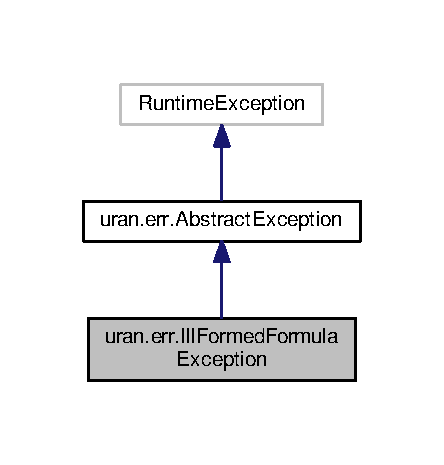
\includegraphics[width=213pt]{classuran_1_1err_1_1_ill_formed_formula_exception__inherit__graph}
\end{center}
\end{figure}


Collaboration diagram for uran.\+err.\+Ill\+Formed\+Formula\+Exception\+:
\nopagebreak
\begin{figure}[H]
\begin{center}
\leavevmode
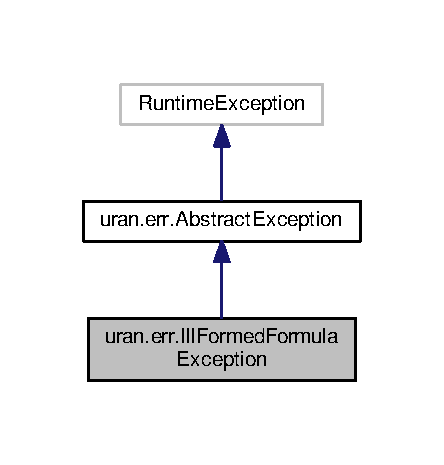
\includegraphics[width=213pt]{classuran_1_1err_1_1_ill_formed_formula_exception__coll__graph}
\end{center}
\end{figure}
\subsection*{Public Member Functions}
\begin{DoxyCompactItemize}
\item 
\hyperlink{classuran_1_1err_1_1_ill_formed_formula_exception_ad0d82c352f9d32d400103d8da1e14620}{Ill\+Formed\+Formula\+Exception} ()
\item 
\hyperlink{classuran_1_1err_1_1_ill_formed_formula_exception_a5292609d2bc61a277f0542c0afd863ee}{Ill\+Formed\+Formula\+Exception} (String msg)
\end{DoxyCompactItemize}
\subsection*{Additional Inherited Members}


\subsection{Detailed Description}


Definition at line 15 of file Ill\+Formed\+Formula\+Exception.\+java.



\subsection{Constructor \& Destructor Documentation}
\hypertarget{classuran_1_1err_1_1_ill_formed_formula_exception_ad0d82c352f9d32d400103d8da1e14620}{}\index{uran\+::err\+::\+Ill\+Formed\+Formula\+Exception@{uran\+::err\+::\+Ill\+Formed\+Formula\+Exception}!Ill\+Formed\+Formula\+Exception@{Ill\+Formed\+Formula\+Exception}}
\index{Ill\+Formed\+Formula\+Exception@{Ill\+Formed\+Formula\+Exception}!uran\+::err\+::\+Ill\+Formed\+Formula\+Exception@{uran\+::err\+::\+Ill\+Formed\+Formula\+Exception}}
\subsubsection[{Ill\+Formed\+Formula\+Exception}]{\setlength{\rightskip}{0pt plus 5cm}uran.\+err.\+Ill\+Formed\+Formula\+Exception.\+Ill\+Formed\+Formula\+Exception (
\begin{DoxyParamCaption}
{}
\end{DoxyParamCaption}
)\hspace{0.3cm}{\ttfamily [inline]}}\label{classuran_1_1err_1_1_ill_formed_formula_exception_ad0d82c352f9d32d400103d8da1e14620}


Definition at line 17 of file Ill\+Formed\+Formula\+Exception.\+java.

\hypertarget{classuran_1_1err_1_1_ill_formed_formula_exception_a5292609d2bc61a277f0542c0afd863ee}{}\index{uran\+::err\+::\+Ill\+Formed\+Formula\+Exception@{uran\+::err\+::\+Ill\+Formed\+Formula\+Exception}!Ill\+Formed\+Formula\+Exception@{Ill\+Formed\+Formula\+Exception}}
\index{Ill\+Formed\+Formula\+Exception@{Ill\+Formed\+Formula\+Exception}!uran\+::err\+::\+Ill\+Formed\+Formula\+Exception@{uran\+::err\+::\+Ill\+Formed\+Formula\+Exception}}
\subsubsection[{Ill\+Formed\+Formula\+Exception}]{\setlength{\rightskip}{0pt plus 5cm}uran.\+err.\+Ill\+Formed\+Formula\+Exception.\+Ill\+Formed\+Formula\+Exception (
\begin{DoxyParamCaption}
\item[{String}]{msg}
\end{DoxyParamCaption}
)\hspace{0.3cm}{\ttfamily [inline]}}\label{classuran_1_1err_1_1_ill_formed_formula_exception_a5292609d2bc61a277f0542c0afd863ee}


Definition at line 22 of file Ill\+Formed\+Formula\+Exception.\+java.



The documentation for this class was generated from the following file\+:\begin{DoxyCompactItemize}
\item 
/home/haowu/uran/src/uran/err/\hyperlink{_ill_formed_formula_exception_8java}{Ill\+Formed\+Formula\+Exception.\+java}\end{DoxyCompactItemize}

\hypertarget{classuran_1_1formula_1_1_implies_formula}{}\section{uran.\+formula.\+Implies\+Formula Class Reference}
\label{classuran_1_1formula_1_1_implies_formula}\index{uran.\+formula.\+Implies\+Formula@{uran.\+formula.\+Implies\+Formula}}


Inheritance diagram for uran.\+formula.\+Implies\+Formula\+:
\nopagebreak
\begin{figure}[H]
\begin{center}
\leavevmode
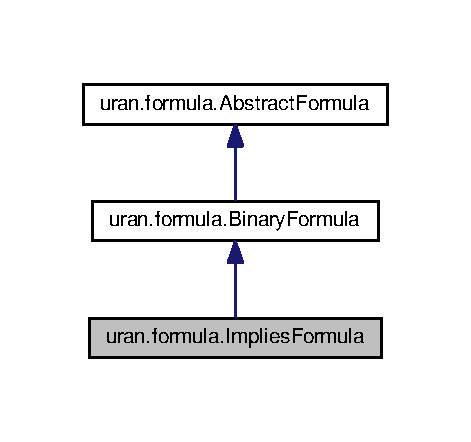
\includegraphics[width=226pt]{classuran_1_1formula_1_1_implies_formula__inherit__graph}
\end{center}
\end{figure}


Collaboration diagram for uran.\+formula.\+Implies\+Formula\+:
\nopagebreak
\begin{figure}[H]
\begin{center}
\leavevmode
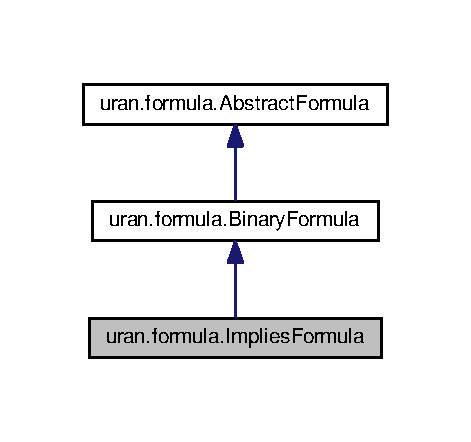
\includegraphics[width=226pt]{classuran_1_1formula_1_1_implies_formula__coll__graph}
\end{center}
\end{figure}
\subsection*{Public Member Functions}
\begin{DoxyCompactItemize}
\item 
\hyperlink{classuran_1_1formula_1_1_implies_formula_a700b2d9ecca6f0fefbe106c7e26abcee}{Implies\+Formula} ()
\item 
\hyperlink{classuran_1_1formula_1_1_implies_formula_aceb28e0de74a0cfc588f920be3fe97b3}{Implies\+Formula} (\hyperlink{classuran_1_1formula_1_1_abstract_formula}{Abstract\+Formula} f1, \hyperlink{classuran_1_1formula_1_1_abstract_formula}{Abstract\+Formula} f2)
\item 
\hyperlink{classuran_1_1formula_1_1_binary_formula}{Binary\+Formula} \hyperlink{classuran_1_1formula_1_1_implies_formula_addbe8bd82d874529f6cdf443f281195f}{merge} (Abstract\+Formula...\+formulas)
\item 
boolean \hyperlink{classuran_1_1formula_1_1_implies_formula_ab71ad72a4ac91c4259a1006a4eee8465}{is\+Implies\+Formula} ()
\end{DoxyCompactItemize}


\subsection{Detailed Description}


Definition at line 19 of file Implies\+Formula.\+java.



\subsection{Constructor \& Destructor Documentation}
\hypertarget{classuran_1_1formula_1_1_implies_formula_a700b2d9ecca6f0fefbe106c7e26abcee}{}\index{uran\+::formula\+::\+Implies\+Formula@{uran\+::formula\+::\+Implies\+Formula}!Implies\+Formula@{Implies\+Formula}}
\index{Implies\+Formula@{Implies\+Formula}!uran\+::formula\+::\+Implies\+Formula@{uran\+::formula\+::\+Implies\+Formula}}
\subsubsection[{Implies\+Formula}]{\setlength{\rightskip}{0pt plus 5cm}uran.\+formula.\+Implies\+Formula.\+Implies\+Formula (
\begin{DoxyParamCaption}
{}
\end{DoxyParamCaption}
)\hspace{0.3cm}{\ttfamily [inline]}}\label{classuran_1_1formula_1_1_implies_formula_a700b2d9ecca6f0fefbe106c7e26abcee}


Definition at line 21 of file Implies\+Formula.\+java.

\hypertarget{classuran_1_1formula_1_1_implies_formula_aceb28e0de74a0cfc588f920be3fe97b3}{}\index{uran\+::formula\+::\+Implies\+Formula@{uran\+::formula\+::\+Implies\+Formula}!Implies\+Formula@{Implies\+Formula}}
\index{Implies\+Formula@{Implies\+Formula}!uran\+::formula\+::\+Implies\+Formula@{uran\+::formula\+::\+Implies\+Formula}}
\subsubsection[{Implies\+Formula}]{\setlength{\rightskip}{0pt plus 5cm}uran.\+formula.\+Implies\+Formula.\+Implies\+Formula (
\begin{DoxyParamCaption}
\item[{{\bf Abstract\+Formula}}]{f1, }
\item[{{\bf Abstract\+Formula}}]{f2}
\end{DoxyParamCaption}
)\hspace{0.3cm}{\ttfamily [inline]}}\label{classuran_1_1formula_1_1_implies_formula_aceb28e0de74a0cfc588f920be3fe97b3}


Definition at line 23 of file Implies\+Formula.\+java.



\subsection{Member Function Documentation}
\hypertarget{classuran_1_1formula_1_1_implies_formula_ab71ad72a4ac91c4259a1006a4eee8465}{}\index{uran\+::formula\+::\+Implies\+Formula@{uran\+::formula\+::\+Implies\+Formula}!is\+Implies\+Formula@{is\+Implies\+Formula}}
\index{is\+Implies\+Formula@{is\+Implies\+Formula}!uran\+::formula\+::\+Implies\+Formula@{uran\+::formula\+::\+Implies\+Formula}}
\subsubsection[{is\+Implies\+Formula}]{\setlength{\rightskip}{0pt plus 5cm}boolean uran.\+formula.\+Implies\+Formula.\+is\+Implies\+Formula (
\begin{DoxyParamCaption}
{}
\end{DoxyParamCaption}
)\hspace{0.3cm}{\ttfamily [inline]}}\label{classuran_1_1formula_1_1_implies_formula_ab71ad72a4ac91c4259a1006a4eee8465}


Definition at line 51 of file Implies\+Formula.\+java.

\hypertarget{classuran_1_1formula_1_1_implies_formula_addbe8bd82d874529f6cdf443f281195f}{}\index{uran\+::formula\+::\+Implies\+Formula@{uran\+::formula\+::\+Implies\+Formula}!merge@{merge}}
\index{merge@{merge}!uran\+::formula\+::\+Implies\+Formula@{uran\+::formula\+::\+Implies\+Formula}}
\subsubsection[{merge}]{\setlength{\rightskip}{0pt plus 5cm}{\bf Binary\+Formula} uran.\+formula.\+Implies\+Formula.\+merge (
\begin{DoxyParamCaption}
\item[{Abstract\+Formula...}]{formulas}
\end{DoxyParamCaption}
)\hspace{0.3cm}{\ttfamily [inline]}}\label{classuran_1_1formula_1_1_implies_formula_addbe8bd82d874529f6cdf443f281195f}


Definition at line 29 of file Implies\+Formula.\+java.



The documentation for this class was generated from the following file\+:\begin{DoxyCompactItemize}
\item 
/home/haowu/uran/src/uran/formula/\hyperlink{_implies_formula_8java}{Implies\+Formula.\+java}\end{DoxyCompactItemize}

\hypertarget{classuran_1_1formula_1_1type_1_1_int}{}\section{uran.\+formula.\+type.\+Int Class Reference}
\label{classuran_1_1formula_1_1type_1_1_int}\index{uran.\+formula.\+type.\+Int@{uran.\+formula.\+type.\+Int}}


Inheritance diagram for uran.\+formula.\+type.\+Int\+:
\nopagebreak
\begin{figure}[H]
\begin{center}
\leavevmode
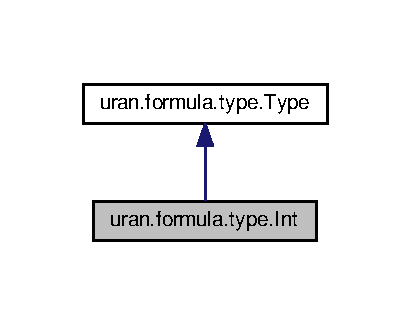
\includegraphics[width=197pt]{classuran_1_1formula_1_1type_1_1_int__inherit__graph}
\end{center}
\end{figure}


Collaboration diagram for uran.\+formula.\+type.\+Int\+:
\nopagebreak
\begin{figure}[H]
\begin{center}
\leavevmode
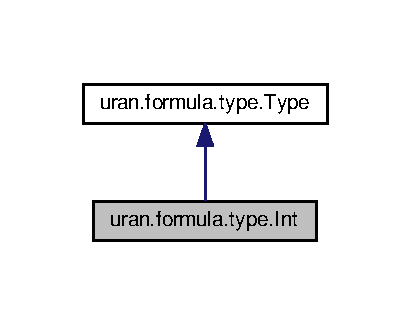
\includegraphics[width=197pt]{classuran_1_1formula_1_1type_1_1_int__coll__graph}
\end{center}
\end{figure}
\subsection*{Public Member Functions}
\begin{DoxyCompactItemize}
\item 
\hyperlink{classuran_1_1formula_1_1type_1_1_int_aea0ad46892976650be418935cbaed096}{Int} ()
\item 
String \hyperlink{classuran_1_1formula_1_1type_1_1_int_ab9e4d8cbc83dab11f15b6d38930f2699}{name} ()
\item 
boolean \hyperlink{classuran_1_1formula_1_1type_1_1_int_aa672bea374613f142e10cf58159e8342}{is\+Int} ()
\item 
String \hyperlink{classuran_1_1formula_1_1type_1_1_int_a51cd4bd2b0dc21484b293994ce070ad5}{to\+String} ()
\end{DoxyCompactItemize}
\subsection*{Additional Inherited Members}


\subsection{Detailed Description}


Definition at line 16 of file Int.\+java.



\subsection{Constructor \& Destructor Documentation}
\hypertarget{classuran_1_1formula_1_1type_1_1_int_aea0ad46892976650be418935cbaed096}{}\index{uran\+::formula\+::type\+::\+Int@{uran\+::formula\+::type\+::\+Int}!Int@{Int}}
\index{Int@{Int}!uran\+::formula\+::type\+::\+Int@{uran\+::formula\+::type\+::\+Int}}
\subsubsection[{Int}]{\setlength{\rightskip}{0pt plus 5cm}uran.\+formula.\+type.\+Int.\+Int (
\begin{DoxyParamCaption}
{}
\end{DoxyParamCaption}
)\hspace{0.3cm}{\ttfamily [inline]}}\label{classuran_1_1formula_1_1type_1_1_int_aea0ad46892976650be418935cbaed096}


Definition at line 18 of file Int.\+java.



\subsection{Member Function Documentation}
\hypertarget{classuran_1_1formula_1_1type_1_1_int_aa672bea374613f142e10cf58159e8342}{}\index{uran\+::formula\+::type\+::\+Int@{uran\+::formula\+::type\+::\+Int}!is\+Int@{is\+Int}}
\index{is\+Int@{is\+Int}!uran\+::formula\+::type\+::\+Int@{uran\+::formula\+::type\+::\+Int}}
\subsubsection[{is\+Int}]{\setlength{\rightskip}{0pt plus 5cm}boolean uran.\+formula.\+type.\+Int.\+is\+Int (
\begin{DoxyParamCaption}
{}
\end{DoxyParamCaption}
)\hspace{0.3cm}{\ttfamily [inline]}}\label{classuran_1_1formula_1_1type_1_1_int_aa672bea374613f142e10cf58159e8342}


Definition at line 28 of file Int.\+java.

\hypertarget{classuran_1_1formula_1_1type_1_1_int_ab9e4d8cbc83dab11f15b6d38930f2699}{}\index{uran\+::formula\+::type\+::\+Int@{uran\+::formula\+::type\+::\+Int}!name@{name}}
\index{name@{name}!uran\+::formula\+::type\+::\+Int@{uran\+::formula\+::type\+::\+Int}}
\subsubsection[{name}]{\setlength{\rightskip}{0pt plus 5cm}String uran.\+formula.\+type.\+Int.\+name (
\begin{DoxyParamCaption}
{}
\end{DoxyParamCaption}
)\hspace{0.3cm}{\ttfamily [inline]}}\label{classuran_1_1formula_1_1type_1_1_int_ab9e4d8cbc83dab11f15b6d38930f2699}


Definition at line 23 of file Int.\+java.

\hypertarget{classuran_1_1formula_1_1type_1_1_int_a51cd4bd2b0dc21484b293994ce070ad5}{}\index{uran\+::formula\+::type\+::\+Int@{uran\+::formula\+::type\+::\+Int}!to\+String@{to\+String}}
\index{to\+String@{to\+String}!uran\+::formula\+::type\+::\+Int@{uran\+::formula\+::type\+::\+Int}}
\subsubsection[{to\+String}]{\setlength{\rightskip}{0pt plus 5cm}String uran.\+formula.\+type.\+Int.\+to\+String (
\begin{DoxyParamCaption}
{}
\end{DoxyParamCaption}
)\hspace{0.3cm}{\ttfamily [inline]}}\label{classuran_1_1formula_1_1type_1_1_int_a51cd4bd2b0dc21484b293994ce070ad5}


Definition at line 30 of file Int.\+java.



The documentation for this class was generated from the following file\+:\begin{DoxyCompactItemize}
\item 
/home/haowu/uran/src/uran/formula/type/\hyperlink{_int_8java}{Int.\+java}\end{DoxyCompactItemize}

\hypertarget{classuran_1_1formula_1_1value_1_1_int_value}{}\section{uran.\+formula.\+value.\+Int\+Value Class Reference}
\label{classuran_1_1formula_1_1value_1_1_int_value}\index{uran.\+formula.\+value.\+Int\+Value@{uran.\+formula.\+value.\+Int\+Value}}


Inheritance diagram for uran.\+formula.\+value.\+Int\+Value\+:
\nopagebreak
\begin{figure}[H]
\begin{center}
\leavevmode
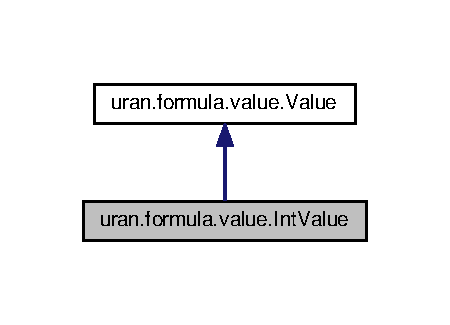
\includegraphics[width=216pt]{classuran_1_1formula_1_1value_1_1_int_value__inherit__graph}
\end{center}
\end{figure}


Collaboration diagram for uran.\+formula.\+value.\+Int\+Value\+:
\nopagebreak
\begin{figure}[H]
\begin{center}
\leavevmode
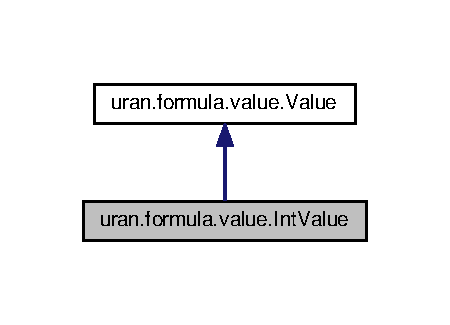
\includegraphics[width=216pt]{classuran_1_1formula_1_1value_1_1_int_value__coll__graph}
\end{center}
\end{figure}
\subsection*{Public Member Functions}
\begin{DoxyCompactItemize}
\item 
\hyperlink{classuran_1_1formula_1_1value_1_1_int_value_a868f41864c99f386416c4ac8ad97ee6f}{Int\+Value} ()
\item 
\hyperlink{classuran_1_1formula_1_1value_1_1_int_value_a4b8929377f8b1695637b44be1dfcb199}{Int\+Value} (int v)
\item 
int \hyperlink{classuran_1_1formula_1_1value_1_1_int_value_a4438dfb13523e3e7a499029fd4b44db0}{get\+Value} ()
\item 
void \hyperlink{classuran_1_1formula_1_1value_1_1_int_value_aeeb25c9d6725ff339155cdbe3beb7ddb}{set\+Value} (int n)
\item 
boolean \hyperlink{classuran_1_1formula_1_1value_1_1_int_value_a2ccb183ca3f2cb38571c7d01ac2a4b12}{Is\+Int} ()
\item 
String \hyperlink{classuran_1_1formula_1_1value_1_1_int_value_ab51e6b6c0ade2614f3abd651ca53ae4b}{to\+String} ()
\end{DoxyCompactItemize}


\subsection{Detailed Description}


Definition at line 15 of file Int\+Value.\+java.



\subsection{Constructor \& Destructor Documentation}
\hypertarget{classuran_1_1formula_1_1value_1_1_int_value_a868f41864c99f386416c4ac8ad97ee6f}{}\index{uran\+::formula\+::value\+::\+Int\+Value@{uran\+::formula\+::value\+::\+Int\+Value}!Int\+Value@{Int\+Value}}
\index{Int\+Value@{Int\+Value}!uran\+::formula\+::value\+::\+Int\+Value@{uran\+::formula\+::value\+::\+Int\+Value}}
\subsubsection[{Int\+Value}]{\setlength{\rightskip}{0pt plus 5cm}uran.\+formula.\+value.\+Int\+Value.\+Int\+Value (
\begin{DoxyParamCaption}
{}
\end{DoxyParamCaption}
)\hspace{0.3cm}{\ttfamily [inline]}}\label{classuran_1_1formula_1_1value_1_1_int_value_a868f41864c99f386416c4ac8ad97ee6f}


Definition at line 17 of file Int\+Value.\+java.

\hypertarget{classuran_1_1formula_1_1value_1_1_int_value_a4b8929377f8b1695637b44be1dfcb199}{}\index{uran\+::formula\+::value\+::\+Int\+Value@{uran\+::formula\+::value\+::\+Int\+Value}!Int\+Value@{Int\+Value}}
\index{Int\+Value@{Int\+Value}!uran\+::formula\+::value\+::\+Int\+Value@{uran\+::formula\+::value\+::\+Int\+Value}}
\subsubsection[{Int\+Value}]{\setlength{\rightskip}{0pt plus 5cm}uran.\+formula.\+value.\+Int\+Value.\+Int\+Value (
\begin{DoxyParamCaption}
\item[{int}]{v}
\end{DoxyParamCaption}
)\hspace{0.3cm}{\ttfamily [inline]}}\label{classuran_1_1formula_1_1value_1_1_int_value_a4b8929377f8b1695637b44be1dfcb199}


Definition at line 18 of file Int\+Value.\+java.



\subsection{Member Function Documentation}
\hypertarget{classuran_1_1formula_1_1value_1_1_int_value_a4438dfb13523e3e7a499029fd4b44db0}{}\index{uran\+::formula\+::value\+::\+Int\+Value@{uran\+::formula\+::value\+::\+Int\+Value}!get\+Value@{get\+Value}}
\index{get\+Value@{get\+Value}!uran\+::formula\+::value\+::\+Int\+Value@{uran\+::formula\+::value\+::\+Int\+Value}}
\subsubsection[{get\+Value}]{\setlength{\rightskip}{0pt plus 5cm}int uran.\+formula.\+value.\+Int\+Value.\+get\+Value (
\begin{DoxyParamCaption}
{}
\end{DoxyParamCaption}
)\hspace{0.3cm}{\ttfamily [inline]}}\label{classuran_1_1formula_1_1value_1_1_int_value_a4438dfb13523e3e7a499029fd4b44db0}


Definition at line 19 of file Int\+Value.\+java.

\hypertarget{classuran_1_1formula_1_1value_1_1_int_value_a2ccb183ca3f2cb38571c7d01ac2a4b12}{}\index{uran\+::formula\+::value\+::\+Int\+Value@{uran\+::formula\+::value\+::\+Int\+Value}!Is\+Int@{Is\+Int}}
\index{Is\+Int@{Is\+Int}!uran\+::formula\+::value\+::\+Int\+Value@{uran\+::formula\+::value\+::\+Int\+Value}}
\subsubsection[{Is\+Int}]{\setlength{\rightskip}{0pt plus 5cm}boolean uran.\+formula.\+value.\+Int\+Value.\+Is\+Int (
\begin{DoxyParamCaption}
{}
\end{DoxyParamCaption}
)\hspace{0.3cm}{\ttfamily [inline]}}\label{classuran_1_1formula_1_1value_1_1_int_value_a2ccb183ca3f2cb38571c7d01ac2a4b12}


Definition at line 21 of file Int\+Value.\+java.

\hypertarget{classuran_1_1formula_1_1value_1_1_int_value_aeeb25c9d6725ff339155cdbe3beb7ddb}{}\index{uran\+::formula\+::value\+::\+Int\+Value@{uran\+::formula\+::value\+::\+Int\+Value}!set\+Value@{set\+Value}}
\index{set\+Value@{set\+Value}!uran\+::formula\+::value\+::\+Int\+Value@{uran\+::formula\+::value\+::\+Int\+Value}}
\subsubsection[{set\+Value}]{\setlength{\rightskip}{0pt plus 5cm}void uran.\+formula.\+value.\+Int\+Value.\+set\+Value (
\begin{DoxyParamCaption}
\item[{int}]{n}
\end{DoxyParamCaption}
)\hspace{0.3cm}{\ttfamily [inline]}}\label{classuran_1_1formula_1_1value_1_1_int_value_aeeb25c9d6725ff339155cdbe3beb7ddb}


Definition at line 20 of file Int\+Value.\+java.

\hypertarget{classuran_1_1formula_1_1value_1_1_int_value_ab51e6b6c0ade2614f3abd651ca53ae4b}{}\index{uran\+::formula\+::value\+::\+Int\+Value@{uran\+::formula\+::value\+::\+Int\+Value}!to\+String@{to\+String}}
\index{to\+String@{to\+String}!uran\+::formula\+::value\+::\+Int\+Value@{uran\+::formula\+::value\+::\+Int\+Value}}
\subsubsection[{to\+String}]{\setlength{\rightskip}{0pt plus 5cm}String uran.\+formula.\+value.\+Int\+Value.\+to\+String (
\begin{DoxyParamCaption}
{}
\end{DoxyParamCaption}
)\hspace{0.3cm}{\ttfamily [inline]}}\label{classuran_1_1formula_1_1value_1_1_int_value_ab51e6b6c0ade2614f3abd651ca53ae4b}


Definition at line 22 of file Int\+Value.\+java.



The documentation for this class was generated from the following file\+:\begin{DoxyCompactItemize}
\item 
/home/haowu/uran/src/uran/formula/value/\hyperlink{_int_value_8java}{Int\+Value.\+java}\end{DoxyCompactItemize}

\hypertarget{classuran_1_1formula_1_1_literal}{}\section{uran.\+formula.\+Literal Class Reference}
\label{classuran_1_1formula_1_1_literal}\index{uran.\+formula.\+Literal@{uran.\+formula.\+Literal}}


Inheritance diagram for uran.\+formula.\+Literal\+:
\nopagebreak
\begin{figure}[H]
\begin{center}
\leavevmode
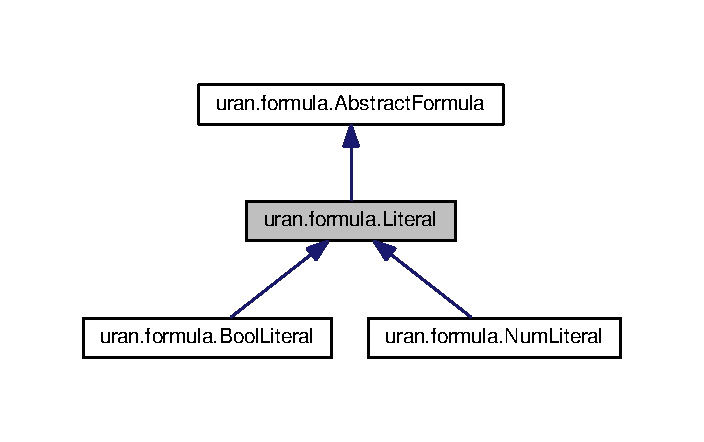
\includegraphics[width=338pt]{classuran_1_1formula_1_1_literal__inherit__graph}
\end{center}
\end{figure}


Collaboration diagram for uran.\+formula.\+Literal\+:
\nopagebreak
\begin{figure}[H]
\begin{center}
\leavevmode
\includegraphics[width=226pt]{classuran_1_1formula_1_1_literal__coll__graph}
\end{center}
\end{figure}
\subsection*{Public Member Functions}
\begin{DoxyCompactItemize}
\item 
boolean \hyperlink{classuran_1_1formula_1_1_literal_aa0f22e354535d5689c0424be804b5990}{is\+Literal} ()
\end{DoxyCompactItemize}


\subsection{Detailed Description}


Definition at line 16 of file Literal.\+java.



\subsection{Member Function Documentation}
\hypertarget{classuran_1_1formula_1_1_literal_aa0f22e354535d5689c0424be804b5990}{}\index{uran\+::formula\+::\+Literal@{uran\+::formula\+::\+Literal}!is\+Literal@{is\+Literal}}
\index{is\+Literal@{is\+Literal}!uran\+::formula\+::\+Literal@{uran\+::formula\+::\+Literal}}
\subsubsection[{is\+Literal}]{\setlength{\rightskip}{0pt plus 5cm}boolean uran.\+formula.\+Literal.\+is\+Literal (
\begin{DoxyParamCaption}
{}
\end{DoxyParamCaption}
)\hspace{0.3cm}{\ttfamily [inline]}}\label{classuran_1_1formula_1_1_literal_aa0f22e354535d5689c0424be804b5990}


Definition at line 19 of file Literal.\+java.



The documentation for this class was generated from the following file\+:\begin{DoxyCompactItemize}
\item 
/home/haowu/uran/src/uran/formula/\hyperlink{_literal_8java}{Literal.\+java}\end{DoxyCompactItemize}

\hypertarget{classuran_1_1err_1_1_miss_file_name_exception}{}\section{uran.\+err.\+Miss\+File\+Name\+Exception Class Reference}
\label{classuran_1_1err_1_1_miss_file_name_exception}\index{uran.\+err.\+Miss\+File\+Name\+Exception@{uran.\+err.\+Miss\+File\+Name\+Exception}}


Inheritance diagram for uran.\+err.\+Miss\+File\+Name\+Exception\+:
\nopagebreak
\begin{figure}[H]
\begin{center}
\leavevmode
\includegraphics[width=239pt]{classuran_1_1err_1_1_miss_file_name_exception__inherit__graph}
\end{center}
\end{figure}


Collaboration diagram for uran.\+err.\+Miss\+File\+Name\+Exception\+:
\nopagebreak
\begin{figure}[H]
\begin{center}
\leavevmode
\includegraphics[width=239pt]{classuran_1_1err_1_1_miss_file_name_exception__coll__graph}
\end{center}
\end{figure}
\subsection*{Public Member Functions}
\begin{DoxyCompactItemize}
\item 
\hyperlink{classuran_1_1err_1_1_miss_file_name_exception_a60c20afd789fa6ded76a2dea6c355829}{Miss\+File\+Name\+Exception} ()
\item 
\hyperlink{classuran_1_1err_1_1_miss_file_name_exception_acdadcc2e7cddfdeedf0144b68ba43a08}{Miss\+File\+Name\+Exception} (String msg)
\end{DoxyCompactItemize}
\subsection*{Additional Inherited Members}


\subsection{Detailed Description}


Definition at line 15 of file Miss\+File\+Name\+Exception.\+java.



\subsection{Constructor \& Destructor Documentation}
\hypertarget{classuran_1_1err_1_1_miss_file_name_exception_a60c20afd789fa6ded76a2dea6c355829}{}\index{uran\+::err\+::\+Miss\+File\+Name\+Exception@{uran\+::err\+::\+Miss\+File\+Name\+Exception}!Miss\+File\+Name\+Exception@{Miss\+File\+Name\+Exception}}
\index{Miss\+File\+Name\+Exception@{Miss\+File\+Name\+Exception}!uran\+::err\+::\+Miss\+File\+Name\+Exception@{uran\+::err\+::\+Miss\+File\+Name\+Exception}}
\subsubsection[{Miss\+File\+Name\+Exception}]{\setlength{\rightskip}{0pt plus 5cm}uran.\+err.\+Miss\+File\+Name\+Exception.\+Miss\+File\+Name\+Exception (
\begin{DoxyParamCaption}
{}
\end{DoxyParamCaption}
)\hspace{0.3cm}{\ttfamily [inline]}}\label{classuran_1_1err_1_1_miss_file_name_exception_a60c20afd789fa6ded76a2dea6c355829}


Definition at line 17 of file Miss\+File\+Name\+Exception.\+java.

\hypertarget{classuran_1_1err_1_1_miss_file_name_exception_acdadcc2e7cddfdeedf0144b68ba43a08}{}\index{uran\+::err\+::\+Miss\+File\+Name\+Exception@{uran\+::err\+::\+Miss\+File\+Name\+Exception}!Miss\+File\+Name\+Exception@{Miss\+File\+Name\+Exception}}
\index{Miss\+File\+Name\+Exception@{Miss\+File\+Name\+Exception}!uran\+::err\+::\+Miss\+File\+Name\+Exception@{uran\+::err\+::\+Miss\+File\+Name\+Exception}}
\subsubsection[{Miss\+File\+Name\+Exception}]{\setlength{\rightskip}{0pt plus 5cm}uran.\+err.\+Miss\+File\+Name\+Exception.\+Miss\+File\+Name\+Exception (
\begin{DoxyParamCaption}
\item[{String}]{msg}
\end{DoxyParamCaption}
)\hspace{0.3cm}{\ttfamily [inline]}}\label{classuran_1_1err_1_1_miss_file_name_exception_acdadcc2e7cddfdeedf0144b68ba43a08}


Definition at line 22 of file Miss\+File\+Name\+Exception.\+java.



The documentation for this class was generated from the following file\+:\begin{DoxyCompactItemize}
\item 
/home/haowu/uran/src/uran/err/\hyperlink{_miss_file_name_exception_8java}{Miss\+File\+Name\+Exception.\+java}\end{DoxyCompactItemize}

\hypertarget{classuran_1_1err_1_1_missing_formula_exception}{}\section{uran.\+err.\+Missing\+Formula\+Exception Class Reference}
\label{classuran_1_1err_1_1_missing_formula_exception}\index{uran.\+err.\+Missing\+Formula\+Exception@{uran.\+err.\+Missing\+Formula\+Exception}}


Inheritance diagram for uran.\+err.\+Missing\+Formula\+Exception\+:
\nopagebreak
\begin{figure}[H]
\begin{center}
\leavevmode
\includegraphics[width=245pt]{classuran_1_1err_1_1_missing_formula_exception__inherit__graph}
\end{center}
\end{figure}


Collaboration diagram for uran.\+err.\+Missing\+Formula\+Exception\+:
\nopagebreak
\begin{figure}[H]
\begin{center}
\leavevmode
\includegraphics[width=245pt]{classuran_1_1err_1_1_missing_formula_exception__coll__graph}
\end{center}
\end{figure}
\subsection*{Public Member Functions}
\begin{DoxyCompactItemize}
\item 
\hyperlink{classuran_1_1err_1_1_missing_formula_exception_a59940e0bc519c837ee89b7376cf0a4c9}{Missing\+Formula\+Exception} ()
\item 
\hyperlink{classuran_1_1err_1_1_missing_formula_exception_a8c65805ccb53cfd402fcd5dabe61a198}{Missing\+Formula\+Exception} (String msg)
\end{DoxyCompactItemize}
\subsection*{Additional Inherited Members}


\subsection{Detailed Description}


Definition at line 15 of file Missing\+Formula\+Exception.\+java.



\subsection{Constructor \& Destructor Documentation}
\hypertarget{classuran_1_1err_1_1_missing_formula_exception_a59940e0bc519c837ee89b7376cf0a4c9}{}\index{uran\+::err\+::\+Missing\+Formula\+Exception@{uran\+::err\+::\+Missing\+Formula\+Exception}!Missing\+Formula\+Exception@{Missing\+Formula\+Exception}}
\index{Missing\+Formula\+Exception@{Missing\+Formula\+Exception}!uran\+::err\+::\+Missing\+Formula\+Exception@{uran\+::err\+::\+Missing\+Formula\+Exception}}
\subsubsection[{Missing\+Formula\+Exception}]{\setlength{\rightskip}{0pt plus 5cm}uran.\+err.\+Missing\+Formula\+Exception.\+Missing\+Formula\+Exception (
\begin{DoxyParamCaption}
{}
\end{DoxyParamCaption}
)\hspace{0.3cm}{\ttfamily [inline]}}\label{classuran_1_1err_1_1_missing_formula_exception_a59940e0bc519c837ee89b7376cf0a4c9}


Definition at line 17 of file Missing\+Formula\+Exception.\+java.

\hypertarget{classuran_1_1err_1_1_missing_formula_exception_a8c65805ccb53cfd402fcd5dabe61a198}{}\index{uran\+::err\+::\+Missing\+Formula\+Exception@{uran\+::err\+::\+Missing\+Formula\+Exception}!Missing\+Formula\+Exception@{Missing\+Formula\+Exception}}
\index{Missing\+Formula\+Exception@{Missing\+Formula\+Exception}!uran\+::err\+::\+Missing\+Formula\+Exception@{uran\+::err\+::\+Missing\+Formula\+Exception}}
\subsubsection[{Missing\+Formula\+Exception}]{\setlength{\rightskip}{0pt plus 5cm}uran.\+err.\+Missing\+Formula\+Exception.\+Missing\+Formula\+Exception (
\begin{DoxyParamCaption}
\item[{String}]{msg}
\end{DoxyParamCaption}
)\hspace{0.3cm}{\ttfamily [inline]}}\label{classuran_1_1err_1_1_missing_formula_exception_a8c65805ccb53cfd402fcd5dabe61a198}


Definition at line 22 of file Missing\+Formula\+Exception.\+java.



The documentation for this class was generated from the following file\+:\begin{DoxyCompactItemize}
\item 
/home/haowu/uran/src/uran/err/\hyperlink{_missing_formula_exception_8java}{Missing\+Formula\+Exception.\+java}\end{DoxyCompactItemize}

\hypertarget{classuran_1_1formula_1_1_neg_formula}{}\section{uran.\+formula.\+Neg\+Formula Class Reference}
\label{classuran_1_1formula_1_1_neg_formula}\index{uran.\+formula.\+Neg\+Formula@{uran.\+formula.\+Neg\+Formula}}


Inheritance diagram for uran.\+formula.\+Neg\+Formula\+:
\nopagebreak
\begin{figure}[H]
\begin{center}
\leavevmode
\includegraphics[width=226pt]{classuran_1_1formula_1_1_neg_formula__inherit__graph}
\end{center}
\end{figure}


Collaboration diagram for uran.\+formula.\+Neg\+Formula\+:
\nopagebreak
\begin{figure}[H]
\begin{center}
\leavevmode
\includegraphics[width=226pt]{classuran_1_1formula_1_1_neg_formula__coll__graph}
\end{center}
\end{figure}
\subsection*{Public Member Functions}
\begin{DoxyCompactItemize}
\item 
\hyperlink{classuran_1_1formula_1_1_neg_formula_a855414617b195187e14ed543d0f5ea22}{Neg\+Formula} (\hyperlink{classuran_1_1formula_1_1_abstract_formula}{Abstract\+Formula} \hyperlink{classuran_1_1formula_1_1_unary_formula_a348d9e263106ff6085e47c01e15737e2}{formula})
\item 
boolean \hyperlink{classuran_1_1formula_1_1_neg_formula_a3a7a64b9a56865fe428bce6489c20e1c}{is\+Neg\+Formula} ()
\item 
String \hyperlink{classuran_1_1formula_1_1_neg_formula_a4449691a30eb46b75d3a06fee65449ad}{to\+String} ()
\item 
String \hyperlink{classuran_1_1formula_1_1_neg_formula_a107330b0c52fa7d51300c1ee835262bd}{to\+S\+M\+T2} ()
\item 
void \hyperlink{classuran_1_1formula_1_1_neg_formula_a33dc4b60c10bbc87c345a8d5b73c8de7}{accept} (\hyperlink{classuran_1_1formula_1_1visitor_1_1_abstract_visitor}{Abstract\+Visitor} visitor)
\end{DoxyCompactItemize}


\subsection{Detailed Description}


Definition at line 17 of file Neg\+Formula.\+java.



\subsection{Constructor \& Destructor Documentation}
\hypertarget{classuran_1_1formula_1_1_neg_formula_a855414617b195187e14ed543d0f5ea22}{}\index{uran\+::formula\+::\+Neg\+Formula@{uran\+::formula\+::\+Neg\+Formula}!Neg\+Formula@{Neg\+Formula}}
\index{Neg\+Formula@{Neg\+Formula}!uran\+::formula\+::\+Neg\+Formula@{uran\+::formula\+::\+Neg\+Formula}}
\subsubsection[{Neg\+Formula}]{\setlength{\rightskip}{0pt plus 5cm}uran.\+formula.\+Neg\+Formula.\+Neg\+Formula (
\begin{DoxyParamCaption}
\item[{{\bf Abstract\+Formula}}]{formula}
\end{DoxyParamCaption}
)\hspace{0.3cm}{\ttfamily [inline]}}\label{classuran_1_1formula_1_1_neg_formula_a855414617b195187e14ed543d0f5ea22}


Definition at line 19 of file Neg\+Formula.\+java.



\subsection{Member Function Documentation}
\hypertarget{classuran_1_1formula_1_1_neg_formula_a33dc4b60c10bbc87c345a8d5b73c8de7}{}\index{uran\+::formula\+::\+Neg\+Formula@{uran\+::formula\+::\+Neg\+Formula}!accept@{accept}}
\index{accept@{accept}!uran\+::formula\+::\+Neg\+Formula@{uran\+::formula\+::\+Neg\+Formula}}
\subsubsection[{accept}]{\setlength{\rightskip}{0pt plus 5cm}void uran.\+formula.\+Neg\+Formula.\+accept (
\begin{DoxyParamCaption}
\item[{{\bf Abstract\+Visitor}}]{visitor}
\end{DoxyParamCaption}
)\hspace{0.3cm}{\ttfamily [inline]}}\label{classuran_1_1formula_1_1_neg_formula_a33dc4b60c10bbc87c345a8d5b73c8de7}


Definition at line 33 of file Neg\+Formula.\+java.

\hypertarget{classuran_1_1formula_1_1_neg_formula_a3a7a64b9a56865fe428bce6489c20e1c}{}\index{uran\+::formula\+::\+Neg\+Formula@{uran\+::formula\+::\+Neg\+Formula}!is\+Neg\+Formula@{is\+Neg\+Formula}}
\index{is\+Neg\+Formula@{is\+Neg\+Formula}!uran\+::formula\+::\+Neg\+Formula@{uran\+::formula\+::\+Neg\+Formula}}
\subsubsection[{is\+Neg\+Formula}]{\setlength{\rightskip}{0pt plus 5cm}boolean uran.\+formula.\+Neg\+Formula.\+is\+Neg\+Formula (
\begin{DoxyParamCaption}
{}
\end{DoxyParamCaption}
)\hspace{0.3cm}{\ttfamily [inline]}}\label{classuran_1_1formula_1_1_neg_formula_a3a7a64b9a56865fe428bce6489c20e1c}


Definition at line 24 of file Neg\+Formula.\+java.

\hypertarget{classuran_1_1formula_1_1_neg_formula_a107330b0c52fa7d51300c1ee835262bd}{}\index{uran\+::formula\+::\+Neg\+Formula@{uran\+::formula\+::\+Neg\+Formula}!to\+S\+M\+T2@{to\+S\+M\+T2}}
\index{to\+S\+M\+T2@{to\+S\+M\+T2}!uran\+::formula\+::\+Neg\+Formula@{uran\+::formula\+::\+Neg\+Formula}}
\subsubsection[{to\+S\+M\+T2}]{\setlength{\rightskip}{0pt plus 5cm}String uran.\+formula.\+Neg\+Formula.\+to\+S\+M\+T2 (
\begin{DoxyParamCaption}
{}
\end{DoxyParamCaption}
)\hspace{0.3cm}{\ttfamily [inline]}}\label{classuran_1_1formula_1_1_neg_formula_a107330b0c52fa7d51300c1ee835262bd}


Definition at line 30 of file Neg\+Formula.\+java.

\hypertarget{classuran_1_1formula_1_1_neg_formula_a4449691a30eb46b75d3a06fee65449ad}{}\index{uran\+::formula\+::\+Neg\+Formula@{uran\+::formula\+::\+Neg\+Formula}!to\+String@{to\+String}}
\index{to\+String@{to\+String}!uran\+::formula\+::\+Neg\+Formula@{uran\+::formula\+::\+Neg\+Formula}}
\subsubsection[{to\+String}]{\setlength{\rightskip}{0pt plus 5cm}String uran.\+formula.\+Neg\+Formula.\+to\+String (
\begin{DoxyParamCaption}
{}
\end{DoxyParamCaption}
)\hspace{0.3cm}{\ttfamily [inline]}}\label{classuran_1_1formula_1_1_neg_formula_a4449691a30eb46b75d3a06fee65449ad}


Definition at line 27 of file Neg\+Formula.\+java.



The documentation for this class was generated from the following file\+:\begin{DoxyCompactItemize}
\item 
/home/haowu/uran/src/uran/formula/\hyperlink{_neg_formula_8java}{Neg\+Formula.\+java}\end{DoxyCompactItemize}

\hypertarget{classuran_1_1formula_1_1cnf_1_1_node}{}\section{uran.\+formula.\+cnf.\+Node Class Reference}
\label{classuran_1_1formula_1_1cnf_1_1_node}\index{uran.\+formula.\+cnf.\+Node@{uran.\+formula.\+cnf.\+Node}}


Inheritance diagram for uran.\+formula.\+cnf.\+Node\+:
\nopagebreak
\begin{figure}[H]
\begin{center}
\leavevmode
\includegraphics[width=350pt]{classuran_1_1formula_1_1cnf_1_1_node__inherit__graph}
\end{center}
\end{figure}
\subsection*{Public Member Functions}
\begin{DoxyCompactItemize}
\item 
String \hyperlink{classuran_1_1formula_1_1cnf_1_1_node_a03afe96d7b3cdb15bd8f018943247b1c}{to\+String} ()
\end{DoxyCompactItemize}


\subsection{Detailed Description}


Definition at line 17 of file Node.\+java.



\subsection{Member Function Documentation}
\hypertarget{classuran_1_1formula_1_1cnf_1_1_node_a03afe96d7b3cdb15bd8f018943247b1c}{}\index{uran\+::formula\+::cnf\+::\+Node@{uran\+::formula\+::cnf\+::\+Node}!to\+String@{to\+String}}
\index{to\+String@{to\+String}!uran\+::formula\+::cnf\+::\+Node@{uran\+::formula\+::cnf\+::\+Node}}
\subsubsection[{to\+String}]{\setlength{\rightskip}{0pt plus 5cm}String uran.\+formula.\+cnf.\+Node.\+to\+String (
\begin{DoxyParamCaption}
{}
\end{DoxyParamCaption}
)\hspace{0.3cm}{\ttfamily [inline]}}\label{classuran_1_1formula_1_1cnf_1_1_node_a03afe96d7b3cdb15bd8f018943247b1c}


Definition at line 19 of file Node.\+java.



The documentation for this class was generated from the following file\+:\begin{DoxyCompactItemize}
\item 
/home/haowu/uran/src/uran/formula/cnf/\hyperlink{_node_8java}{Node.\+java}\end{DoxyCompactItemize}

\hypertarget{classuran_1_1formula_1_1cnf_1_1_not_gate}{}\section{uran.\+formula.\+cnf.\+Not\+Gate Class Reference}
\label{classuran_1_1formula_1_1cnf_1_1_not_gate}\index{uran.\+formula.\+cnf.\+Not\+Gate@{uran.\+formula.\+cnf.\+Not\+Gate}}


Inheritance diagram for uran.\+formula.\+cnf.\+Not\+Gate\+:
\nopagebreak
\begin{figure}[H]
\begin{center}
\leavevmode
\includegraphics[width=207pt]{classuran_1_1formula_1_1cnf_1_1_not_gate__inherit__graph}
\end{center}
\end{figure}


Collaboration diagram for uran.\+formula.\+cnf.\+Not\+Gate\+:
\nopagebreak
\begin{figure}[H]
\begin{center}
\leavevmode
\includegraphics[width=207pt]{classuran_1_1formula_1_1cnf_1_1_not_gate__coll__graph}
\end{center}
\end{figure}
\subsection*{Public Member Functions}
\begin{DoxyCompactItemize}
\item 
\hyperlink{classuran_1_1formula_1_1cnf_1_1_not_gate_ae9dab1d0cf160cde169bcdb0661197e4}{Not\+Gate} (\hyperlink{classuran_1_1formula_1_1cnf_1_1_boolean_circuit}{Boolean\+Circuit} i)
\item 
\hyperlink{classuran_1_1formula_1_1cnf_1_1_boolean_circuit}{Boolean\+Circuit} \hyperlink{classuran_1_1formula_1_1cnf_1_1_not_gate_aea0f0b1a1aa6cc41437e863b4b1e969d}{input} ()
\item 
boolean \hyperlink{classuran_1_1formula_1_1cnf_1_1_not_gate_a5cce395bd78d29b0bc6356fb2a52af5c}{is\+Not\+Gate} ()
\item 
void \hyperlink{classuran_1_1formula_1_1cnf_1_1_not_gate_a46df11a9a00f7a81e1838b2001167385}{accept} (\hyperlink{classuran_1_1formula_1_1cnf_1_1visitor_1_1_abstract_visitor}{Abstract\+Visitor} v)
\end{DoxyCompactItemize}
\subsection*{Additional Inherited Members}


\subsection{Detailed Description}


Definition at line 18 of file Not\+Gate.\+java.



\subsection{Constructor \& Destructor Documentation}
\hypertarget{classuran_1_1formula_1_1cnf_1_1_not_gate_ae9dab1d0cf160cde169bcdb0661197e4}{}\index{uran\+::formula\+::cnf\+::\+Not\+Gate@{uran\+::formula\+::cnf\+::\+Not\+Gate}!Not\+Gate@{Not\+Gate}}
\index{Not\+Gate@{Not\+Gate}!uran\+::formula\+::cnf\+::\+Not\+Gate@{uran\+::formula\+::cnf\+::\+Not\+Gate}}
\subsubsection[{Not\+Gate}]{\setlength{\rightskip}{0pt plus 5cm}uran.\+formula.\+cnf.\+Not\+Gate.\+Not\+Gate (
\begin{DoxyParamCaption}
\item[{{\bf Boolean\+Circuit}}]{i}
\end{DoxyParamCaption}
)\hspace{0.3cm}{\ttfamily [inline]}}\label{classuran_1_1formula_1_1cnf_1_1_not_gate_ae9dab1d0cf160cde169bcdb0661197e4}


Definition at line 22 of file Not\+Gate.\+java.



\subsection{Member Function Documentation}
\hypertarget{classuran_1_1formula_1_1cnf_1_1_not_gate_a46df11a9a00f7a81e1838b2001167385}{}\index{uran\+::formula\+::cnf\+::\+Not\+Gate@{uran\+::formula\+::cnf\+::\+Not\+Gate}!accept@{accept}}
\index{accept@{accept}!uran\+::formula\+::cnf\+::\+Not\+Gate@{uran\+::formula\+::cnf\+::\+Not\+Gate}}
\subsubsection[{accept}]{\setlength{\rightskip}{0pt plus 5cm}void uran.\+formula.\+cnf.\+Not\+Gate.\+accept (
\begin{DoxyParamCaption}
\item[{{\bf Abstract\+Visitor}}]{v}
\end{DoxyParamCaption}
)\hspace{0.3cm}{\ttfamily [inline]}}\label{classuran_1_1formula_1_1cnf_1_1_not_gate_a46df11a9a00f7a81e1838b2001167385}


Definition at line 31 of file Not\+Gate.\+java.

\hypertarget{classuran_1_1formula_1_1cnf_1_1_not_gate_aea0f0b1a1aa6cc41437e863b4b1e969d}{}\index{uran\+::formula\+::cnf\+::\+Not\+Gate@{uran\+::formula\+::cnf\+::\+Not\+Gate}!input@{input}}
\index{input@{input}!uran\+::formula\+::cnf\+::\+Not\+Gate@{uran\+::formula\+::cnf\+::\+Not\+Gate}}
\subsubsection[{input}]{\setlength{\rightskip}{0pt plus 5cm}{\bf Boolean\+Circuit} uran.\+formula.\+cnf.\+Not\+Gate.\+input (
\begin{DoxyParamCaption}
{}
\end{DoxyParamCaption}
)\hspace{0.3cm}{\ttfamily [inline]}}\label{classuran_1_1formula_1_1cnf_1_1_not_gate_aea0f0b1a1aa6cc41437e863b4b1e969d}


Definition at line 26 of file Not\+Gate.\+java.

\hypertarget{classuran_1_1formula_1_1cnf_1_1_not_gate_a5cce395bd78d29b0bc6356fb2a52af5c}{}\index{uran\+::formula\+::cnf\+::\+Not\+Gate@{uran\+::formula\+::cnf\+::\+Not\+Gate}!is\+Not\+Gate@{is\+Not\+Gate}}
\index{is\+Not\+Gate@{is\+Not\+Gate}!uran\+::formula\+::cnf\+::\+Not\+Gate@{uran\+::formula\+::cnf\+::\+Not\+Gate}}
\subsubsection[{is\+Not\+Gate}]{\setlength{\rightskip}{0pt plus 5cm}boolean uran.\+formula.\+cnf.\+Not\+Gate.\+is\+Not\+Gate (
\begin{DoxyParamCaption}
{}
\end{DoxyParamCaption}
)\hspace{0.3cm}{\ttfamily [inline]}}\label{classuran_1_1formula_1_1cnf_1_1_not_gate_a5cce395bd78d29b0bc6356fb2a52af5c}


Definition at line 30 of file Not\+Gate.\+java.



The documentation for this class was generated from the following file\+:\begin{DoxyCompactItemize}
\item 
/home/haowu/uran/src/uran/formula/cnf/\hyperlink{_not_gate_8java}{Not\+Gate.\+java}\end{DoxyCompactItemize}

\hypertarget{classuran_1_1err_1_1_nullable_formula_exception}{}\section{uran.\+err.\+Nullable\+Formula\+Exception Class Reference}
\label{classuran_1_1err_1_1_nullable_formula_exception}\index{uran.\+err.\+Nullable\+Formula\+Exception@{uran.\+err.\+Nullable\+Formula\+Exception}}


Inheritance diagram for uran.\+err.\+Nullable\+Formula\+Exception\+:
\nopagebreak
\begin{figure}[H]
\begin{center}
\leavevmode
\includegraphics[width=213pt]{classuran_1_1err_1_1_nullable_formula_exception__inherit__graph}
\end{center}
\end{figure}


Collaboration diagram for uran.\+err.\+Nullable\+Formula\+Exception\+:
\nopagebreak
\begin{figure}[H]
\begin{center}
\leavevmode
\includegraphics[width=213pt]{classuran_1_1err_1_1_nullable_formula_exception__coll__graph}
\end{center}
\end{figure}
\subsection*{Public Member Functions}
\begin{DoxyCompactItemize}
\item 
\hyperlink{classuran_1_1err_1_1_nullable_formula_exception_a633e11f1ea429102c42ae027966b60aa}{Nullable\+Formula\+Exception} ()
\item 
\hyperlink{classuran_1_1err_1_1_nullable_formula_exception_a79cee869d400a09840fba1a74e02e296}{Nullable\+Formula\+Exception} (String msg)
\end{DoxyCompactItemize}
\subsection*{Additional Inherited Members}


\subsection{Detailed Description}


Definition at line 15 of file Nullable\+Formula\+Exception.\+java.



\subsection{Constructor \& Destructor Documentation}
\hypertarget{classuran_1_1err_1_1_nullable_formula_exception_a633e11f1ea429102c42ae027966b60aa}{}\index{uran\+::err\+::\+Nullable\+Formula\+Exception@{uran\+::err\+::\+Nullable\+Formula\+Exception}!Nullable\+Formula\+Exception@{Nullable\+Formula\+Exception}}
\index{Nullable\+Formula\+Exception@{Nullable\+Formula\+Exception}!uran\+::err\+::\+Nullable\+Formula\+Exception@{uran\+::err\+::\+Nullable\+Formula\+Exception}}
\subsubsection[{Nullable\+Formula\+Exception}]{\setlength{\rightskip}{0pt plus 5cm}uran.\+err.\+Nullable\+Formula\+Exception.\+Nullable\+Formula\+Exception (
\begin{DoxyParamCaption}
{}
\end{DoxyParamCaption}
)\hspace{0.3cm}{\ttfamily [inline]}}\label{classuran_1_1err_1_1_nullable_formula_exception_a633e11f1ea429102c42ae027966b60aa}


Definition at line 17 of file Nullable\+Formula\+Exception.\+java.

\hypertarget{classuran_1_1err_1_1_nullable_formula_exception_a79cee869d400a09840fba1a74e02e296}{}\index{uran\+::err\+::\+Nullable\+Formula\+Exception@{uran\+::err\+::\+Nullable\+Formula\+Exception}!Nullable\+Formula\+Exception@{Nullable\+Formula\+Exception}}
\index{Nullable\+Formula\+Exception@{Nullable\+Formula\+Exception}!uran\+::err\+::\+Nullable\+Formula\+Exception@{uran\+::err\+::\+Nullable\+Formula\+Exception}}
\subsubsection[{Nullable\+Formula\+Exception}]{\setlength{\rightskip}{0pt plus 5cm}uran.\+err.\+Nullable\+Formula\+Exception.\+Nullable\+Formula\+Exception (
\begin{DoxyParamCaption}
\item[{String}]{msg}
\end{DoxyParamCaption}
)\hspace{0.3cm}{\ttfamily [inline]}}\label{classuran_1_1err_1_1_nullable_formula_exception_a79cee869d400a09840fba1a74e02e296}


Definition at line 22 of file Nullable\+Formula\+Exception.\+java.



The documentation for this class was generated from the following file\+:\begin{DoxyCompactItemize}
\item 
/home/haowu/uran/src/uran/err/\hyperlink{_nullable_formula_exception_8java}{Nullable\+Formula\+Exception.\+java}\end{DoxyCompactItemize}

\hypertarget{classuran_1_1formula_1_1_num_literal}{}\section{uran.\+formula.\+Num\+Literal Class Reference}
\label{classuran_1_1formula_1_1_num_literal}\index{uran.\+formula.\+Num\+Literal@{uran.\+formula.\+Num\+Literal}}


Inheritance diagram for uran.\+formula.\+Num\+Literal\+:
\nopagebreak
\begin{figure}[H]
\begin{center}
\leavevmode
\includegraphics[width=226pt]{classuran_1_1formula_1_1_num_literal__inherit__graph}
\end{center}
\end{figure}


Collaboration diagram for uran.\+formula.\+Num\+Literal\+:
\nopagebreak
\begin{figure}[H]
\begin{center}
\leavevmode
\includegraphics[width=226pt]{classuran_1_1formula_1_1_num_literal__coll__graph}
\end{center}
\end{figure}
\subsection*{Public Member Functions}
\begin{DoxyCompactItemize}
\item 
\hyperlink{classuran_1_1formula_1_1_num_literal_ab5f51d42c30b78bb92d0f81b11de74b2}{Num\+Literal} ()
\item 
\hyperlink{classuran_1_1formula_1_1_num_literal_adbe8e877d682a661601384af835fb00c}{Num\+Literal} (\hyperlink{classuran_1_1formula_1_1value_1_1_int_value}{Int\+Value} v)
\item 
\hyperlink{classuran_1_1formula_1_1_num_literal_a333acaa358eab1eb223f272ff2b4e9bb}{Num\+Literal} (int v)
\item 
\hyperlink{classuran_1_1formula_1_1value_1_1_int_value}{Int\+Value} \hyperlink{classuran_1_1formula_1_1_num_literal_ae0dadbefcc69349f5bd80fbf9140001a}{get\+Value} ()
\item 
int \hyperlink{classuran_1_1formula_1_1_num_literal_a79f2cf4b24ef2e670a574787bd308954}{get\+Literal} ()
\item 
String \hyperlink{classuran_1_1formula_1_1_num_literal_abf0b7431a2da3673ce8af875f66dc159}{to\+String} ()
\item 
String \hyperlink{classuran_1_1formula_1_1_num_literal_a09557ce20900450f1263e672a90cd5c6}{to\+S\+M\+T2} ()
\item 
void \hyperlink{classuran_1_1formula_1_1_num_literal_a2756adaea87c705446096fcebb6a04ac}{accept} (\hyperlink{classuran_1_1formula_1_1visitor_1_1_abstract_visitor}{Abstract\+Visitor} visitor)
\end{DoxyCompactItemize}


\subsection{Detailed Description}
Numeric \hyperlink{classuran_1_1formula_1_1_literal}{Literal} 

Definition at line 18 of file Num\+Literal.\+java.



\subsection{Constructor \& Destructor Documentation}
\hypertarget{classuran_1_1formula_1_1_num_literal_ab5f51d42c30b78bb92d0f81b11de74b2}{}\index{uran\+::formula\+::\+Num\+Literal@{uran\+::formula\+::\+Num\+Literal}!Num\+Literal@{Num\+Literal}}
\index{Num\+Literal@{Num\+Literal}!uran\+::formula\+::\+Num\+Literal@{uran\+::formula\+::\+Num\+Literal}}
\subsubsection[{Num\+Literal}]{\setlength{\rightskip}{0pt plus 5cm}uran.\+formula.\+Num\+Literal.\+Num\+Literal (
\begin{DoxyParamCaption}
{}
\end{DoxyParamCaption}
)\hspace{0.3cm}{\ttfamily [inline]}}\label{classuran_1_1formula_1_1_num_literal_ab5f51d42c30b78bb92d0f81b11de74b2}


Definition at line 22 of file Num\+Literal.\+java.

\hypertarget{classuran_1_1formula_1_1_num_literal_adbe8e877d682a661601384af835fb00c}{}\index{uran\+::formula\+::\+Num\+Literal@{uran\+::formula\+::\+Num\+Literal}!Num\+Literal@{Num\+Literal}}
\index{Num\+Literal@{Num\+Literal}!uran\+::formula\+::\+Num\+Literal@{uran\+::formula\+::\+Num\+Literal}}
\subsubsection[{Num\+Literal}]{\setlength{\rightskip}{0pt plus 5cm}uran.\+formula.\+Num\+Literal.\+Num\+Literal (
\begin{DoxyParamCaption}
\item[{{\bf Int\+Value}}]{v}
\end{DoxyParamCaption}
)\hspace{0.3cm}{\ttfamily [inline]}}\label{classuran_1_1formula_1_1_num_literal_adbe8e877d682a661601384af835fb00c}


Definition at line 28 of file Num\+Literal.\+java.

\hypertarget{classuran_1_1formula_1_1_num_literal_a333acaa358eab1eb223f272ff2b4e9bb}{}\index{uran\+::formula\+::\+Num\+Literal@{uran\+::formula\+::\+Num\+Literal}!Num\+Literal@{Num\+Literal}}
\index{Num\+Literal@{Num\+Literal}!uran\+::formula\+::\+Num\+Literal@{uran\+::formula\+::\+Num\+Literal}}
\subsubsection[{Num\+Literal}]{\setlength{\rightskip}{0pt plus 5cm}uran.\+formula.\+Num\+Literal.\+Num\+Literal (
\begin{DoxyParamCaption}
\item[{int}]{v}
\end{DoxyParamCaption}
)\hspace{0.3cm}{\ttfamily [inline]}}\label{classuran_1_1formula_1_1_num_literal_a333acaa358eab1eb223f272ff2b4e9bb}
Take an integer as a numeric constant 

Definition at line 33 of file Num\+Literal.\+java.



\subsection{Member Function Documentation}
\hypertarget{classuran_1_1formula_1_1_num_literal_a2756adaea87c705446096fcebb6a04ac}{}\index{uran\+::formula\+::\+Num\+Literal@{uran\+::formula\+::\+Num\+Literal}!accept@{accept}}
\index{accept@{accept}!uran\+::formula\+::\+Num\+Literal@{uran\+::formula\+::\+Num\+Literal}}
\subsubsection[{accept}]{\setlength{\rightskip}{0pt plus 5cm}void uran.\+formula.\+Num\+Literal.\+accept (
\begin{DoxyParamCaption}
\item[{{\bf Abstract\+Visitor}}]{visitor}
\end{DoxyParamCaption}
)\hspace{0.3cm}{\ttfamily [inline]}}\label{classuran_1_1formula_1_1_num_literal_a2756adaea87c705446096fcebb6a04ac}


Definition at line 54 of file Num\+Literal.\+java.

\hypertarget{classuran_1_1formula_1_1_num_literal_a79f2cf4b24ef2e670a574787bd308954}{}\index{uran\+::formula\+::\+Num\+Literal@{uran\+::formula\+::\+Num\+Literal}!get\+Literal@{get\+Literal}}
\index{get\+Literal@{get\+Literal}!uran\+::formula\+::\+Num\+Literal@{uran\+::formula\+::\+Num\+Literal}}
\subsubsection[{get\+Literal}]{\setlength{\rightskip}{0pt plus 5cm}int uran.\+formula.\+Num\+Literal.\+get\+Literal (
\begin{DoxyParamCaption}
{}
\end{DoxyParamCaption}
)\hspace{0.3cm}{\ttfamily [inline]}}\label{classuran_1_1formula_1_1_num_literal_a79f2cf4b24ef2e670a574787bd308954}


Definition at line 41 of file Num\+Literal.\+java.

\hypertarget{classuran_1_1formula_1_1_num_literal_ae0dadbefcc69349f5bd80fbf9140001a}{}\index{uran\+::formula\+::\+Num\+Literal@{uran\+::formula\+::\+Num\+Literal}!get\+Value@{get\+Value}}
\index{get\+Value@{get\+Value}!uran\+::formula\+::\+Num\+Literal@{uran\+::formula\+::\+Num\+Literal}}
\subsubsection[{get\+Value}]{\setlength{\rightskip}{0pt plus 5cm}{\bf Int\+Value} uran.\+formula.\+Num\+Literal.\+get\+Value (
\begin{DoxyParamCaption}
{}
\end{DoxyParamCaption}
)\hspace{0.3cm}{\ttfamily [inline]}}\label{classuran_1_1formula_1_1_num_literal_ae0dadbefcc69349f5bd80fbf9140001a}


Definition at line 37 of file Num\+Literal.\+java.

\hypertarget{classuran_1_1formula_1_1_num_literal_a09557ce20900450f1263e672a90cd5c6}{}\index{uran\+::formula\+::\+Num\+Literal@{uran\+::formula\+::\+Num\+Literal}!to\+S\+M\+T2@{to\+S\+M\+T2}}
\index{to\+S\+M\+T2@{to\+S\+M\+T2}!uran\+::formula\+::\+Num\+Literal@{uran\+::formula\+::\+Num\+Literal}}
\subsubsection[{to\+S\+M\+T2}]{\setlength{\rightskip}{0pt plus 5cm}String uran.\+formula.\+Num\+Literal.\+to\+S\+M\+T2 (
\begin{DoxyParamCaption}
{}
\end{DoxyParamCaption}
)\hspace{0.3cm}{\ttfamily [inline]}}\label{classuran_1_1formula_1_1_num_literal_a09557ce20900450f1263e672a90cd5c6}


Definition at line 51 of file Num\+Literal.\+java.

\hypertarget{classuran_1_1formula_1_1_num_literal_abf0b7431a2da3673ce8af875f66dc159}{}\index{uran\+::formula\+::\+Num\+Literal@{uran\+::formula\+::\+Num\+Literal}!to\+String@{to\+String}}
\index{to\+String@{to\+String}!uran\+::formula\+::\+Num\+Literal@{uran\+::formula\+::\+Num\+Literal}}
\subsubsection[{to\+String}]{\setlength{\rightskip}{0pt plus 5cm}String uran.\+formula.\+Num\+Literal.\+to\+String (
\begin{DoxyParamCaption}
{}
\end{DoxyParamCaption}
)\hspace{0.3cm}{\ttfamily [inline]}}\label{classuran_1_1formula_1_1_num_literal_abf0b7431a2da3673ce8af875f66dc159}


Definition at line 46 of file Num\+Literal.\+java.



The documentation for this class was generated from the following file\+:\begin{DoxyCompactItemize}
\item 
/home/haowu/uran/src/uran/formula/\hyperlink{_num_literal_8java}{Num\+Literal.\+java}\end{DoxyCompactItemize}

\hypertarget{classuran_1_1formula_1_1_one_formula}{}\section{uran.\+formula.\+One\+Formula Class Reference}
\label{classuran_1_1formula_1_1_one_formula}\index{uran.\+formula.\+One\+Formula@{uran.\+formula.\+One\+Formula}}


Inheritance diagram for uran.\+formula.\+One\+Formula\+:
\nopagebreak
\begin{figure}[H]
\begin{center}
\leavevmode
\includegraphics[width=226pt]{classuran_1_1formula_1_1_one_formula__inherit__graph}
\end{center}
\end{figure}


Collaboration diagram for uran.\+formula.\+One\+Formula\+:
\nopagebreak
\begin{figure}[H]
\begin{center}
\leavevmode
\includegraphics[width=226pt]{classuran_1_1formula_1_1_one_formula__coll__graph}
\end{center}
\end{figure}
\subsection*{Public Member Functions}
\begin{DoxyCompactItemize}
\item 
\hyperlink{classuran_1_1formula_1_1_one_formula_a895932f8a44e8a21fc6a646b07228b2c}{One\+Formula} ()
\item 
\hyperlink{classuran_1_1formula_1_1_one_formula_a25348c1946b818dd97b52666aa9e201b}{One\+Formula} (\hyperlink{classuran_1_1formula_1_1_abstract_formula}{Abstract\+Formula} f1, \hyperlink{classuran_1_1formula_1_1_abstract_formula}{Abstract\+Formula} f2)
\item 
\hyperlink{classuran_1_1formula_1_1_binary_formula}{Binary\+Formula} \hyperlink{classuran_1_1formula_1_1_one_formula_afcb3982b108b0af41e49e67f11dcd4ce}{merge} (Abstract\+Formula...\+formulas)
\end{DoxyCompactItemize}


\subsection{Detailed Description}


Definition at line 20 of file One\+Formula.\+java.



\subsection{Constructor \& Destructor Documentation}
\hypertarget{classuran_1_1formula_1_1_one_formula_a895932f8a44e8a21fc6a646b07228b2c}{}\index{uran\+::formula\+::\+One\+Formula@{uran\+::formula\+::\+One\+Formula}!One\+Formula@{One\+Formula}}
\index{One\+Formula@{One\+Formula}!uran\+::formula\+::\+One\+Formula@{uran\+::formula\+::\+One\+Formula}}
\subsubsection[{One\+Formula}]{\setlength{\rightskip}{0pt plus 5cm}uran.\+formula.\+One\+Formula.\+One\+Formula (
\begin{DoxyParamCaption}
{}
\end{DoxyParamCaption}
)\hspace{0.3cm}{\ttfamily [inline]}}\label{classuran_1_1formula_1_1_one_formula_a895932f8a44e8a21fc6a646b07228b2c}


Definition at line 22 of file One\+Formula.\+java.

\hypertarget{classuran_1_1formula_1_1_one_formula_a25348c1946b818dd97b52666aa9e201b}{}\index{uran\+::formula\+::\+One\+Formula@{uran\+::formula\+::\+One\+Formula}!One\+Formula@{One\+Formula}}
\index{One\+Formula@{One\+Formula}!uran\+::formula\+::\+One\+Formula@{uran\+::formula\+::\+One\+Formula}}
\subsubsection[{One\+Formula}]{\setlength{\rightskip}{0pt plus 5cm}uran.\+formula.\+One\+Formula.\+One\+Formula (
\begin{DoxyParamCaption}
\item[{{\bf Abstract\+Formula}}]{f1, }
\item[{{\bf Abstract\+Formula}}]{f2}
\end{DoxyParamCaption}
)\hspace{0.3cm}{\ttfamily [inline]}}\label{classuran_1_1formula_1_1_one_formula_a25348c1946b818dd97b52666aa9e201b}


Definition at line 24 of file One\+Formula.\+java.



\subsection{Member Function Documentation}
\hypertarget{classuran_1_1formula_1_1_one_formula_afcb3982b108b0af41e49e67f11dcd4ce}{}\index{uran\+::formula\+::\+One\+Formula@{uran\+::formula\+::\+One\+Formula}!merge@{merge}}
\index{merge@{merge}!uran\+::formula\+::\+One\+Formula@{uran\+::formula\+::\+One\+Formula}}
\subsubsection[{merge}]{\setlength{\rightskip}{0pt plus 5cm}{\bf Binary\+Formula} uran.\+formula.\+One\+Formula.\+merge (
\begin{DoxyParamCaption}
\item[{Abstract\+Formula...}]{formulas}
\end{DoxyParamCaption}
)\hspace{0.3cm}{\ttfamily [inline]}}\label{classuran_1_1formula_1_1_one_formula_afcb3982b108b0af41e49e67f11dcd4ce}


Definition at line 32 of file One\+Formula.\+java.



The documentation for this class was generated from the following file\+:\begin{DoxyCompactItemize}
\item 
/home/haowu/uran/src/uran/formula/\hyperlink{_one_formula_8java}{One\+Formula.\+java}\end{DoxyCompactItemize}

\hypertarget{classuran_1_1formula_1_1cnf_1_1_operator}{}\section{uran.\+formula.\+cnf.\+Operator Class Reference}
\label{classuran_1_1formula_1_1cnf_1_1_operator}\index{uran.\+formula.\+cnf.\+Operator@{uran.\+formula.\+cnf.\+Operator}}


Inheritance diagram for uran.\+formula.\+cnf.\+Operator\+:
\nopagebreak
\begin{figure}[H]
\begin{center}
\leavevmode
\includegraphics[width=208pt]{classuran_1_1formula_1_1cnf_1_1_operator__inherit__graph}
\end{center}
\end{figure}


Collaboration diagram for uran.\+formula.\+cnf.\+Operator\+:
\nopagebreak
\begin{figure}[H]
\begin{center}
\leavevmode
\includegraphics[width=208pt]{classuran_1_1formula_1_1cnf_1_1_operator__coll__graph}
\end{center}
\end{figure}
\subsection*{Static Public Attributes}
\begin{DoxyCompactItemize}
\item 
static final int \hyperlink{classuran_1_1formula_1_1cnf_1_1_operator_a9bee6266cf9d7e2d096db33f4750c9fb}{A\+N\+D} =0
\item 
static final int \hyperlink{classuran_1_1formula_1_1cnf_1_1_operator_a7eeacb98b5e73c0caf9a889a7afcea42}{O\+R} =1
\item 
static final int \hyperlink{classuran_1_1formula_1_1cnf_1_1_operator_ac5089b57e3d7cf6e5bb6e10e2d294c10}{N\+O\+T} =2
\item 
static final int \hyperlink{classuran_1_1formula_1_1cnf_1_1_operator_a0925040ebdb1c6b2ce586ec42212797a}{X\+O\+R} =3
\item 
static final int \hyperlink{classuran_1_1formula_1_1cnf_1_1_operator_a8bdc77e0c28cfc549be4294e6ea28cbb}{N\+A\+N\+D} =4
\item 
static final int \hyperlink{classuran_1_1formula_1_1cnf_1_1_operator_a54f41b26960fc82d4248547d293c8989}{N\+O\+R} =5
\end{DoxyCompactItemize}
\subsection*{Additional Inherited Members}


\subsection{Detailed Description}


Definition at line 17 of file Operator.\+java.



\subsection{Member Data Documentation}
\hypertarget{classuran_1_1formula_1_1cnf_1_1_operator_a9bee6266cf9d7e2d096db33f4750c9fb}{}\index{uran\+::formula\+::cnf\+::\+Operator@{uran\+::formula\+::cnf\+::\+Operator}!A\+N\+D@{A\+N\+D}}
\index{A\+N\+D@{A\+N\+D}!uran\+::formula\+::cnf\+::\+Operator@{uran\+::formula\+::cnf\+::\+Operator}}
\subsubsection[{A\+N\+D}]{\setlength{\rightskip}{0pt plus 5cm}final int uran.\+formula.\+cnf.\+Operator.\+A\+N\+D =0\hspace{0.3cm}{\ttfamily [static]}}\label{classuran_1_1formula_1_1cnf_1_1_operator_a9bee6266cf9d7e2d096db33f4750c9fb}


Definition at line 34 of file Operator.\+java.

\hypertarget{classuran_1_1formula_1_1cnf_1_1_operator_a8bdc77e0c28cfc549be4294e6ea28cbb}{}\index{uran\+::formula\+::cnf\+::\+Operator@{uran\+::formula\+::cnf\+::\+Operator}!N\+A\+N\+D@{N\+A\+N\+D}}
\index{N\+A\+N\+D@{N\+A\+N\+D}!uran\+::formula\+::cnf\+::\+Operator@{uran\+::formula\+::cnf\+::\+Operator}}
\subsubsection[{N\+A\+N\+D}]{\setlength{\rightskip}{0pt plus 5cm}final int uran.\+formula.\+cnf.\+Operator.\+N\+A\+N\+D =4\hspace{0.3cm}{\ttfamily [static]}}\label{classuran_1_1formula_1_1cnf_1_1_operator_a8bdc77e0c28cfc549be4294e6ea28cbb}


Definition at line 38 of file Operator.\+java.

\hypertarget{classuran_1_1formula_1_1cnf_1_1_operator_a54f41b26960fc82d4248547d293c8989}{}\index{uran\+::formula\+::cnf\+::\+Operator@{uran\+::formula\+::cnf\+::\+Operator}!N\+O\+R@{N\+O\+R}}
\index{N\+O\+R@{N\+O\+R}!uran\+::formula\+::cnf\+::\+Operator@{uran\+::formula\+::cnf\+::\+Operator}}
\subsubsection[{N\+O\+R}]{\setlength{\rightskip}{0pt plus 5cm}final int uran.\+formula.\+cnf.\+Operator.\+N\+O\+R =5\hspace{0.3cm}{\ttfamily [static]}}\label{classuran_1_1formula_1_1cnf_1_1_operator_a54f41b26960fc82d4248547d293c8989}


Definition at line 39 of file Operator.\+java.

\hypertarget{classuran_1_1formula_1_1cnf_1_1_operator_ac5089b57e3d7cf6e5bb6e10e2d294c10}{}\index{uran\+::formula\+::cnf\+::\+Operator@{uran\+::formula\+::cnf\+::\+Operator}!N\+O\+T@{N\+O\+T}}
\index{N\+O\+T@{N\+O\+T}!uran\+::formula\+::cnf\+::\+Operator@{uran\+::formula\+::cnf\+::\+Operator}}
\subsubsection[{N\+O\+T}]{\setlength{\rightskip}{0pt plus 5cm}final int uran.\+formula.\+cnf.\+Operator.\+N\+O\+T =2\hspace{0.3cm}{\ttfamily [static]}}\label{classuran_1_1formula_1_1cnf_1_1_operator_ac5089b57e3d7cf6e5bb6e10e2d294c10}


Definition at line 36 of file Operator.\+java.

\hypertarget{classuran_1_1formula_1_1cnf_1_1_operator_a7eeacb98b5e73c0caf9a889a7afcea42}{}\index{uran\+::formula\+::cnf\+::\+Operator@{uran\+::formula\+::cnf\+::\+Operator}!O\+R@{O\+R}}
\index{O\+R@{O\+R}!uran\+::formula\+::cnf\+::\+Operator@{uran\+::formula\+::cnf\+::\+Operator}}
\subsubsection[{O\+R}]{\setlength{\rightskip}{0pt plus 5cm}final int uran.\+formula.\+cnf.\+Operator.\+O\+R =1\hspace{0.3cm}{\ttfamily [static]}}\label{classuran_1_1formula_1_1cnf_1_1_operator_a7eeacb98b5e73c0caf9a889a7afcea42}


Definition at line 35 of file Operator.\+java.

\hypertarget{classuran_1_1formula_1_1cnf_1_1_operator_a0925040ebdb1c6b2ce586ec42212797a}{}\index{uran\+::formula\+::cnf\+::\+Operator@{uran\+::formula\+::cnf\+::\+Operator}!X\+O\+R@{X\+O\+R}}
\index{X\+O\+R@{X\+O\+R}!uran\+::formula\+::cnf\+::\+Operator@{uran\+::formula\+::cnf\+::\+Operator}}
\subsubsection[{X\+O\+R}]{\setlength{\rightskip}{0pt plus 5cm}final int uran.\+formula.\+cnf.\+Operator.\+X\+O\+R =3\hspace{0.3cm}{\ttfamily [static]}}\label{classuran_1_1formula_1_1cnf_1_1_operator_a0925040ebdb1c6b2ce586ec42212797a}


Definition at line 37 of file Operator.\+java.



The documentation for this class was generated from the following file\+:\begin{DoxyCompactItemize}
\item 
/home/haowu/uran/src/uran/formula/cnf/\hyperlink{_operator_8java}{Operator.\+java}\end{DoxyCompactItemize}

\hypertarget{classuran_1_1formula_1_1_or_formula}{}\section{uran.\+formula.\+Or\+Formula Class Reference}
\label{classuran_1_1formula_1_1_or_formula}\index{uran.\+formula.\+Or\+Formula@{uran.\+formula.\+Or\+Formula}}


Inheritance diagram for uran.\+formula.\+Or\+Formula\+:
\nopagebreak
\begin{figure}[H]
\begin{center}
\leavevmode
\includegraphics[width=226pt]{classuran_1_1formula_1_1_or_formula__inherit__graph}
\end{center}
\end{figure}


Collaboration diagram for uran.\+formula.\+Or\+Formula\+:
\nopagebreak
\begin{figure}[H]
\begin{center}
\leavevmode
\includegraphics[width=226pt]{classuran_1_1formula_1_1_or_formula__coll__graph}
\end{center}
\end{figure}
\subsection*{Public Member Functions}
\begin{DoxyCompactItemize}
\item 
\hyperlink{classuran_1_1formula_1_1_or_formula_ac25efe8c60104baa63864650d70f1ef3}{Or\+Formula} ()
\item 
\hyperlink{classuran_1_1formula_1_1_or_formula_a948900d397c74388d80c51ec7d22fab9}{Or\+Formula} (\hyperlink{classuran_1_1formula_1_1_abstract_formula}{Abstract\+Formula} f1, \hyperlink{classuran_1_1formula_1_1_abstract_formula}{Abstract\+Formula} f2)
\item 
\hyperlink{classuran_1_1formula_1_1_or_formula}{Or\+Formula} \hyperlink{classuran_1_1formula_1_1_or_formula_a64d0a95e8ec1a5cd46d6e4fbe2aac07f}{merge} (Abstract\+Formula...\+formulas)
\end{DoxyCompactItemize}


\subsection{Detailed Description}


Definition at line 19 of file Or\+Formula.\+java.



\subsection{Constructor \& Destructor Documentation}
\hypertarget{classuran_1_1formula_1_1_or_formula_ac25efe8c60104baa63864650d70f1ef3}{}\index{uran\+::formula\+::\+Or\+Formula@{uran\+::formula\+::\+Or\+Formula}!Or\+Formula@{Or\+Formula}}
\index{Or\+Formula@{Or\+Formula}!uran\+::formula\+::\+Or\+Formula@{uran\+::formula\+::\+Or\+Formula}}
\subsubsection[{Or\+Formula}]{\setlength{\rightskip}{0pt plus 5cm}uran.\+formula.\+Or\+Formula.\+Or\+Formula (
\begin{DoxyParamCaption}
{}
\end{DoxyParamCaption}
)\hspace{0.3cm}{\ttfamily [inline]}}\label{classuran_1_1formula_1_1_or_formula_ac25efe8c60104baa63864650d70f1ef3}


Definition at line 21 of file Or\+Formula.\+java.

\hypertarget{classuran_1_1formula_1_1_or_formula_a948900d397c74388d80c51ec7d22fab9}{}\index{uran\+::formula\+::\+Or\+Formula@{uran\+::formula\+::\+Or\+Formula}!Or\+Formula@{Or\+Formula}}
\index{Or\+Formula@{Or\+Formula}!uran\+::formula\+::\+Or\+Formula@{uran\+::formula\+::\+Or\+Formula}}
\subsubsection[{Or\+Formula}]{\setlength{\rightskip}{0pt plus 5cm}uran.\+formula.\+Or\+Formula.\+Or\+Formula (
\begin{DoxyParamCaption}
\item[{{\bf Abstract\+Formula}}]{f1, }
\item[{{\bf Abstract\+Formula}}]{f2}
\end{DoxyParamCaption}
)\hspace{0.3cm}{\ttfamily [inline]}}\label{classuran_1_1formula_1_1_or_formula_a948900d397c74388d80c51ec7d22fab9}


Definition at line 23 of file Or\+Formula.\+java.



\subsection{Member Function Documentation}
\hypertarget{classuran_1_1formula_1_1_or_formula_a64d0a95e8ec1a5cd46d6e4fbe2aac07f}{}\index{uran\+::formula\+::\+Or\+Formula@{uran\+::formula\+::\+Or\+Formula}!merge@{merge}}
\index{merge@{merge}!uran\+::formula\+::\+Or\+Formula@{uran\+::formula\+::\+Or\+Formula}}
\subsubsection[{merge}]{\setlength{\rightskip}{0pt plus 5cm}{\bf Or\+Formula} uran.\+formula.\+Or\+Formula.\+merge (
\begin{DoxyParamCaption}
\item[{Abstract\+Formula...}]{formulas}
\end{DoxyParamCaption}
)\hspace{0.3cm}{\ttfamily [inline]}}\label{classuran_1_1formula_1_1_or_formula_a64d0a95e8ec1a5cd46d6e4fbe2aac07f}


Definition at line 29 of file Or\+Formula.\+java.



The documentation for this class was generated from the following file\+:\begin{DoxyCompactItemize}
\item 
/home/haowu/uran/src/uran/formula/\hyperlink{_or_formula_8java}{Or\+Formula.\+java}\end{DoxyCompactItemize}

\hypertarget{classuran_1_1formula_1_1_quantified_formula}{}\section{uran.\+formula.\+Quantified\+Formula Class Reference}
\label{classuran_1_1formula_1_1_quantified_formula}\index{uran.\+formula.\+Quantified\+Formula@{uran.\+formula.\+Quantified\+Formula}}


Inheritance diagram for uran.\+formula.\+Quantified\+Formula\+:
\nopagebreak
\begin{figure}[H]
\begin{center}
\leavevmode
\includegraphics[width=233pt]{classuran_1_1formula_1_1_quantified_formula__inherit__graph}
\end{center}
\end{figure}


Collaboration diagram for uran.\+formula.\+Quantified\+Formula\+:
\nopagebreak
\begin{figure}[H]
\begin{center}
\leavevmode
\includegraphics[width=350pt]{classuran_1_1formula_1_1_quantified_formula__coll__graph}
\end{center}
\end{figure}
\subsection*{Public Member Functions}
\begin{DoxyCompactItemize}
\item 
\hyperlink{classuran_1_1formula_1_1_quantified_formula_a62bf822a56af8cbe293dfed514daeb00}{Quantified\+Formula} (\hyperlink{enumuran_1_1formula_1_1_quantifier}{Quantifier} q, \hyperlink{classuran_1_1formula_1_1_decls}{Decls} d, \hyperlink{classuran_1_1formula_1_1_abstract_formula}{Abstract\+Formula} f)
\item 
\hyperlink{enumuran_1_1formula_1_1_quantifier}{Quantifier} \hyperlink{classuran_1_1formula_1_1_quantified_formula_ac3902f85e5e672c7bfda0f21d1795b11}{get\+Quantifier} ()
\item 
\hyperlink{classuran_1_1formula_1_1_abstract_formula}{Abstract\+Formula} \hyperlink{classuran_1_1formula_1_1_quantified_formula_ae5c041f859073ed83b59097ed891e6ea}{get\+Formula} ()
\item 
\hyperlink{classuran_1_1formula_1_1_constant}{Constant}\mbox{[}$\,$\mbox{]} \hyperlink{classuran_1_1formula_1_1_quantified_formula_af7d03640bc1b5607bb52b4ac45ccb407}{get\+Variables} ()
\item 
\hyperlink{classuran_1_1formula_1_1_decls}{Decls} \hyperlink{classuran_1_1formula_1_1_quantified_formula_a8317aff58070511e4c8422cdec888b8b}{get\+Decls} ()
\item 
void \hyperlink{classuran_1_1formula_1_1_quantified_formula_a30287599a1eae9eccf9c8e10f03a9118}{set\+Variables} (\hyperlink{classuran_1_1formula_1_1_decls}{Decls} d)
\item 
void \hyperlink{classuran_1_1formula_1_1_quantified_formula_a183b4f1493c01f0f86222af4abae6206}{set\+Formula} (\hyperlink{classuran_1_1formula_1_1_abstract_formula}{Abstract\+Formula} f)
\item 
boolean \hyperlink{classuran_1_1formula_1_1_quantified_formula_a7c3b3c56b76f1957659e84e6f22002e8}{is\+Quantified\+Formula} ()
\item 
String \hyperlink{classuran_1_1formula_1_1_quantified_formula_a467f75acab697e225daea1f69a8185d1}{to\+String} ()
\item 
String \hyperlink{classuran_1_1formula_1_1_quantified_formula_acbdb69517ff551437becaf17ebbb1f92}{to\+S\+M\+T2} ()
\item 
void \hyperlink{classuran_1_1formula_1_1_quantified_formula_a39abdfb0445fbb284b82ffcc6942654d}{accept} (\hyperlink{classuran_1_1formula_1_1visitor_1_1_abstract_visitor}{Abstract\+Visitor} visitor)
\end{DoxyCompactItemize}


\subsection{Detailed Description}


Definition at line 18 of file Quantified\+Formula.\+java.



\subsection{Constructor \& Destructor Documentation}
\hypertarget{classuran_1_1formula_1_1_quantified_formula_a62bf822a56af8cbe293dfed514daeb00}{}\index{uran\+::formula\+::\+Quantified\+Formula@{uran\+::formula\+::\+Quantified\+Formula}!Quantified\+Formula@{Quantified\+Formula}}
\index{Quantified\+Formula@{Quantified\+Formula}!uran\+::formula\+::\+Quantified\+Formula@{uran\+::formula\+::\+Quantified\+Formula}}
\subsubsection[{Quantified\+Formula}]{\setlength{\rightskip}{0pt plus 5cm}uran.\+formula.\+Quantified\+Formula.\+Quantified\+Formula (
\begin{DoxyParamCaption}
\item[{{\bf Quantifier}}]{q, }
\item[{{\bf Decls}}]{d, }
\item[{{\bf Abstract\+Formula}}]{f}
\end{DoxyParamCaption}
)\hspace{0.3cm}{\ttfamily [inline]}}\label{classuran_1_1formula_1_1_quantified_formula_a62bf822a56af8cbe293dfed514daeb00}


Definition at line 23 of file Quantified\+Formula.\+java.



\subsection{Member Function Documentation}
\hypertarget{classuran_1_1formula_1_1_quantified_formula_a39abdfb0445fbb284b82ffcc6942654d}{}\index{uran\+::formula\+::\+Quantified\+Formula@{uran\+::formula\+::\+Quantified\+Formula}!accept@{accept}}
\index{accept@{accept}!uran\+::formula\+::\+Quantified\+Formula@{uran\+::formula\+::\+Quantified\+Formula}}
\subsubsection[{accept}]{\setlength{\rightskip}{0pt plus 5cm}void uran.\+formula.\+Quantified\+Formula.\+accept (
\begin{DoxyParamCaption}
\item[{{\bf Abstract\+Visitor}}]{visitor}
\end{DoxyParamCaption}
)\hspace{0.3cm}{\ttfamily [inline]}}\label{classuran_1_1formula_1_1_quantified_formula_a39abdfb0445fbb284b82ffcc6942654d}


Definition at line 56 of file Quantified\+Formula.\+java.

\hypertarget{classuran_1_1formula_1_1_quantified_formula_a8317aff58070511e4c8422cdec888b8b}{}\index{uran\+::formula\+::\+Quantified\+Formula@{uran\+::formula\+::\+Quantified\+Formula}!get\+Decls@{get\+Decls}}
\index{get\+Decls@{get\+Decls}!uran\+::formula\+::\+Quantified\+Formula@{uran\+::formula\+::\+Quantified\+Formula}}
\subsubsection[{get\+Decls}]{\setlength{\rightskip}{0pt plus 5cm}{\bf Decls} uran.\+formula.\+Quantified\+Formula.\+get\+Decls (
\begin{DoxyParamCaption}
{}
\end{DoxyParamCaption}
)\hspace{0.3cm}{\ttfamily [inline]}}\label{classuran_1_1formula_1_1_quantified_formula_a8317aff58070511e4c8422cdec888b8b}


Definition at line 32 of file Quantified\+Formula.\+java.

\hypertarget{classuran_1_1formula_1_1_quantified_formula_ae5c041f859073ed83b59097ed891e6ea}{}\index{uran\+::formula\+::\+Quantified\+Formula@{uran\+::formula\+::\+Quantified\+Formula}!get\+Formula@{get\+Formula}}
\index{get\+Formula@{get\+Formula}!uran\+::formula\+::\+Quantified\+Formula@{uran\+::formula\+::\+Quantified\+Formula}}
\subsubsection[{get\+Formula}]{\setlength{\rightskip}{0pt plus 5cm}{\bf Abstract\+Formula} uran.\+formula.\+Quantified\+Formula.\+get\+Formula (
\begin{DoxyParamCaption}
{}
\end{DoxyParamCaption}
)\hspace{0.3cm}{\ttfamily [inline]}}\label{classuran_1_1formula_1_1_quantified_formula_ae5c041f859073ed83b59097ed891e6ea}


Definition at line 30 of file Quantified\+Formula.\+java.

\hypertarget{classuran_1_1formula_1_1_quantified_formula_ac3902f85e5e672c7bfda0f21d1795b11}{}\index{uran\+::formula\+::\+Quantified\+Formula@{uran\+::formula\+::\+Quantified\+Formula}!get\+Quantifier@{get\+Quantifier}}
\index{get\+Quantifier@{get\+Quantifier}!uran\+::formula\+::\+Quantified\+Formula@{uran\+::formula\+::\+Quantified\+Formula}}
\subsubsection[{get\+Quantifier}]{\setlength{\rightskip}{0pt plus 5cm}{\bf Quantifier} uran.\+formula.\+Quantified\+Formula.\+get\+Quantifier (
\begin{DoxyParamCaption}
{}
\end{DoxyParamCaption}
)\hspace{0.3cm}{\ttfamily [inline]}}\label{classuran_1_1formula_1_1_quantified_formula_ac3902f85e5e672c7bfda0f21d1795b11}


Definition at line 29 of file Quantified\+Formula.\+java.

\hypertarget{classuran_1_1formula_1_1_quantified_formula_af7d03640bc1b5607bb52b4ac45ccb407}{}\index{uran\+::formula\+::\+Quantified\+Formula@{uran\+::formula\+::\+Quantified\+Formula}!get\+Variables@{get\+Variables}}
\index{get\+Variables@{get\+Variables}!uran\+::formula\+::\+Quantified\+Formula@{uran\+::formula\+::\+Quantified\+Formula}}
\subsubsection[{get\+Variables}]{\setlength{\rightskip}{0pt plus 5cm}{\bf Constant} \mbox{[}$\,$\mbox{]} uran.\+formula.\+Quantified\+Formula.\+get\+Variables (
\begin{DoxyParamCaption}
{}
\end{DoxyParamCaption}
)\hspace{0.3cm}{\ttfamily [inline]}}\label{classuran_1_1formula_1_1_quantified_formula_af7d03640bc1b5607bb52b4ac45ccb407}


Definition at line 31 of file Quantified\+Formula.\+java.

\hypertarget{classuran_1_1formula_1_1_quantified_formula_a7c3b3c56b76f1957659e84e6f22002e8}{}\index{uran\+::formula\+::\+Quantified\+Formula@{uran\+::formula\+::\+Quantified\+Formula}!is\+Quantified\+Formula@{is\+Quantified\+Formula}}
\index{is\+Quantified\+Formula@{is\+Quantified\+Formula}!uran\+::formula\+::\+Quantified\+Formula@{uran\+::formula\+::\+Quantified\+Formula}}
\subsubsection[{is\+Quantified\+Formula}]{\setlength{\rightskip}{0pt plus 5cm}boolean uran.\+formula.\+Quantified\+Formula.\+is\+Quantified\+Formula (
\begin{DoxyParamCaption}
{}
\end{DoxyParamCaption}
)\hspace{0.3cm}{\ttfamily [inline]}}\label{classuran_1_1formula_1_1_quantified_formula_a7c3b3c56b76f1957659e84e6f22002e8}


Definition at line 37 of file Quantified\+Formula.\+java.

\hypertarget{classuran_1_1formula_1_1_quantified_formula_a183b4f1493c01f0f86222af4abae6206}{}\index{uran\+::formula\+::\+Quantified\+Formula@{uran\+::formula\+::\+Quantified\+Formula}!set\+Formula@{set\+Formula}}
\index{set\+Formula@{set\+Formula}!uran\+::formula\+::\+Quantified\+Formula@{uran\+::formula\+::\+Quantified\+Formula}}
\subsubsection[{set\+Formula}]{\setlength{\rightskip}{0pt plus 5cm}void uran.\+formula.\+Quantified\+Formula.\+set\+Formula (
\begin{DoxyParamCaption}
\item[{{\bf Abstract\+Formula}}]{f}
\end{DoxyParamCaption}
)\hspace{0.3cm}{\ttfamily [inline]}}\label{classuran_1_1formula_1_1_quantified_formula_a183b4f1493c01f0f86222af4abae6206}


Definition at line 34 of file Quantified\+Formula.\+java.

\hypertarget{classuran_1_1formula_1_1_quantified_formula_a30287599a1eae9eccf9c8e10f03a9118}{}\index{uran\+::formula\+::\+Quantified\+Formula@{uran\+::formula\+::\+Quantified\+Formula}!set\+Variables@{set\+Variables}}
\index{set\+Variables@{set\+Variables}!uran\+::formula\+::\+Quantified\+Formula@{uran\+::formula\+::\+Quantified\+Formula}}
\subsubsection[{set\+Variables}]{\setlength{\rightskip}{0pt plus 5cm}void uran.\+formula.\+Quantified\+Formula.\+set\+Variables (
\begin{DoxyParamCaption}
\item[{{\bf Decls}}]{d}
\end{DoxyParamCaption}
)\hspace{0.3cm}{\ttfamily [inline]}}\label{classuran_1_1formula_1_1_quantified_formula_a30287599a1eae9eccf9c8e10f03a9118}


Definition at line 33 of file Quantified\+Formula.\+java.

\hypertarget{classuran_1_1formula_1_1_quantified_formula_acbdb69517ff551437becaf17ebbb1f92}{}\index{uran\+::formula\+::\+Quantified\+Formula@{uran\+::formula\+::\+Quantified\+Formula}!to\+S\+M\+T2@{to\+S\+M\+T2}}
\index{to\+S\+M\+T2@{to\+S\+M\+T2}!uran\+::formula\+::\+Quantified\+Formula@{uran\+::formula\+::\+Quantified\+Formula}}
\subsubsection[{to\+S\+M\+T2}]{\setlength{\rightskip}{0pt plus 5cm}String uran.\+formula.\+Quantified\+Formula.\+to\+S\+M\+T2 (
\begin{DoxyParamCaption}
{}
\end{DoxyParamCaption}
)\hspace{0.3cm}{\ttfamily [inline]}}\label{classuran_1_1formula_1_1_quantified_formula_acbdb69517ff551437becaf17ebbb1f92}


Definition at line 45 of file Quantified\+Formula.\+java.

\hypertarget{classuran_1_1formula_1_1_quantified_formula_a467f75acab697e225daea1f69a8185d1}{}\index{uran\+::formula\+::\+Quantified\+Formula@{uran\+::formula\+::\+Quantified\+Formula}!to\+String@{to\+String}}
\index{to\+String@{to\+String}!uran\+::formula\+::\+Quantified\+Formula@{uran\+::formula\+::\+Quantified\+Formula}}
\subsubsection[{to\+String}]{\setlength{\rightskip}{0pt plus 5cm}String uran.\+formula.\+Quantified\+Formula.\+to\+String (
\begin{DoxyParamCaption}
{}
\end{DoxyParamCaption}
)\hspace{0.3cm}{\ttfamily [inline]}}\label{classuran_1_1formula_1_1_quantified_formula_a467f75acab697e225daea1f69a8185d1}


Definition at line 40 of file Quantified\+Formula.\+java.



The documentation for this class was generated from the following file\+:\begin{DoxyCompactItemize}
\item 
/home/haowu/uran/src/uran/formula/\hyperlink{_quantified_formula_8java}{Quantified\+Formula.\+java}\end{DoxyCompactItemize}

\hypertarget{enumuran_1_1formula_1_1_quantifier}{}\section{uran.\+formula.\+Quantifier Enum Reference}
\label{enumuran_1_1formula_1_1_quantifier}\index{uran.\+formula.\+Quantifier@{uran.\+formula.\+Quantifier}}


\subsection{Detailed Description}


Definition at line 15 of file Quantifier.\+java.



The documentation for this enum was generated from the following file\+:\begin{DoxyCompactItemize}
\item 
/home/haowu/uran/src/uran/formula/\hyperlink{_quantifier_8java}{Quantifier.\+java}\end{DoxyCompactItemize}

\hypertarget{classuran_1_1formula_1_1type_1_1_real}{}\section{uran.\+formula.\+type.\+Real Class Reference}
\label{classuran_1_1formula_1_1type_1_1_real}\index{uran.\+formula.\+type.\+Real@{uran.\+formula.\+type.\+Real}}


Inheritance diagram for uran.\+formula.\+type.\+Real\+:
\nopagebreak
\begin{figure}[H]
\begin{center}
\leavevmode
\includegraphics[width=197pt]{classuran_1_1formula_1_1type_1_1_real__inherit__graph}
\end{center}
\end{figure}


Collaboration diagram for uran.\+formula.\+type.\+Real\+:
\nopagebreak
\begin{figure}[H]
\begin{center}
\leavevmode
\includegraphics[width=197pt]{classuran_1_1formula_1_1type_1_1_real__coll__graph}
\end{center}
\end{figure}
\subsection*{Public Member Functions}
\begin{DoxyCompactItemize}
\item 
\hyperlink{classuran_1_1formula_1_1type_1_1_real_a46c3843518e927e8d9d5c50e6f9bb513}{Real} ()
\item 
String \hyperlink{classuran_1_1formula_1_1type_1_1_real_a2504c50ccca8fc93c3bb2de0858c5827}{name} ()
\item 
boolean \hyperlink{classuran_1_1formula_1_1type_1_1_real_a6b2087ef3a458ad634d3600728824d64}{is\+Real} ()
\item 
String \hyperlink{classuran_1_1formula_1_1type_1_1_real_a414c34bdb423a31cc4d6f7eb10547700}{to\+String} ()
\end{DoxyCompactItemize}
\subsection*{Additional Inherited Members}


\subsection{Detailed Description}


Definition at line 16 of file Real.\+java.



\subsection{Constructor \& Destructor Documentation}
\hypertarget{classuran_1_1formula_1_1type_1_1_real_a46c3843518e927e8d9d5c50e6f9bb513}{}\index{uran\+::formula\+::type\+::\+Real@{uran\+::formula\+::type\+::\+Real}!Real@{Real}}
\index{Real@{Real}!uran\+::formula\+::type\+::\+Real@{uran\+::formula\+::type\+::\+Real}}
\subsubsection[{Real}]{\setlength{\rightskip}{0pt plus 5cm}uran.\+formula.\+type.\+Real.\+Real (
\begin{DoxyParamCaption}
{}
\end{DoxyParamCaption}
)\hspace{0.3cm}{\ttfamily [inline]}}\label{classuran_1_1formula_1_1type_1_1_real_a46c3843518e927e8d9d5c50e6f9bb513}


Definition at line 18 of file Real.\+java.



\subsection{Member Function Documentation}
\hypertarget{classuran_1_1formula_1_1type_1_1_real_a6b2087ef3a458ad634d3600728824d64}{}\index{uran\+::formula\+::type\+::\+Real@{uran\+::formula\+::type\+::\+Real}!is\+Real@{is\+Real}}
\index{is\+Real@{is\+Real}!uran\+::formula\+::type\+::\+Real@{uran\+::formula\+::type\+::\+Real}}
\subsubsection[{is\+Real}]{\setlength{\rightskip}{0pt plus 5cm}boolean uran.\+formula.\+type.\+Real.\+is\+Real (
\begin{DoxyParamCaption}
{}
\end{DoxyParamCaption}
)\hspace{0.3cm}{\ttfamily [inline]}}\label{classuran_1_1formula_1_1type_1_1_real_a6b2087ef3a458ad634d3600728824d64}


Definition at line 28 of file Real.\+java.

\hypertarget{classuran_1_1formula_1_1type_1_1_real_a2504c50ccca8fc93c3bb2de0858c5827}{}\index{uran\+::formula\+::type\+::\+Real@{uran\+::formula\+::type\+::\+Real}!name@{name}}
\index{name@{name}!uran\+::formula\+::type\+::\+Real@{uran\+::formula\+::type\+::\+Real}}
\subsubsection[{name}]{\setlength{\rightskip}{0pt plus 5cm}String uran.\+formula.\+type.\+Real.\+name (
\begin{DoxyParamCaption}
{}
\end{DoxyParamCaption}
)\hspace{0.3cm}{\ttfamily [inline]}}\label{classuran_1_1formula_1_1type_1_1_real_a2504c50ccca8fc93c3bb2de0858c5827}


Definition at line 23 of file Real.\+java.

\hypertarget{classuran_1_1formula_1_1type_1_1_real_a414c34bdb423a31cc4d6f7eb10547700}{}\index{uran\+::formula\+::type\+::\+Real@{uran\+::formula\+::type\+::\+Real}!to\+String@{to\+String}}
\index{to\+String@{to\+String}!uran\+::formula\+::type\+::\+Real@{uran\+::formula\+::type\+::\+Real}}
\subsubsection[{to\+String}]{\setlength{\rightskip}{0pt plus 5cm}String uran.\+formula.\+type.\+Real.\+to\+String (
\begin{DoxyParamCaption}
{}
\end{DoxyParamCaption}
)\hspace{0.3cm}{\ttfamily [inline]}}\label{classuran_1_1formula_1_1type_1_1_real_a414c34bdb423a31cc4d6f7eb10547700}


Definition at line 30 of file Real.\+java.



The documentation for this class was generated from the following file\+:\begin{DoxyCompactItemize}
\item 
/home/haowu/uran/src/uran/formula/type/\hyperlink{_real_8java}{Real.\+java}\end{DoxyCompactItemize}

\hypertarget{enumuran_1_1solver_1_1_result}{}\section{uran.\+solver.\+Result Enum Reference}
\label{enumuran_1_1solver_1_1_result}\index{uran.\+solver.\+Result@{uran.\+solver.\+Result}}
\subsection*{Public Attributes}
\begin{DoxyCompactItemize}
\item 
\hyperlink{enumuran_1_1solver_1_1_result_ae60a826562b5a59b39d64833ea6420d8}{to\+String}
\end{DoxyCompactItemize}


\subsection{Detailed Description}


Definition at line 15 of file Result.\+java.



\subsection{Member Data Documentation}
\hypertarget{enumuran_1_1solver_1_1_result_ae60a826562b5a59b39d64833ea6420d8}{}\index{uran\+::solver\+::\+Result@{uran\+::solver\+::\+Result}!to\+String@{to\+String}}
\index{to\+String@{to\+String}!uran\+::solver\+::\+Result@{uran\+::solver\+::\+Result}}
\subsubsection[{to\+String}]{\setlength{\rightskip}{0pt plus 5cm}uran.\+solver.\+Result.\+to\+String}\label{enumuran_1_1solver_1_1_result_ae60a826562b5a59b39d64833ea6420d8}
{\bfseries Initial value\+:}
\begin{DoxyCode}
=()\{\textcolor{keywordflow}{return} \textcolor{stringliteral}{"sat"};\}\},
    UNSAT \{\textcolor{keyword}{public} String \hyperlink{enumuran_1_1solver_1_1_result_ae60a826562b5a59b39d64833ea6420d8}{toString}()\{\textcolor{keywordflow}{return} \textcolor{stringliteral}{"unsat"};\}\},
    UNKNOWN \{\textcolor{keyword}{public} String \hyperlink{enumuran_1_1solver_1_1_result_ae60a826562b5a59b39d64833ea6420d8}{toString}()\{\textcolor{keywordflow}{return} \textcolor{stringliteral}{"unkown"};\}\}
\end{DoxyCode}


Definition at line 16 of file Result.\+java.



The documentation for this enum was generated from the following file\+:\begin{DoxyCompactItemize}
\item 
/home/haowu/uran/src/uran/solver/\hyperlink{_result_8java}{Result.\+java}\end{DoxyCompactItemize}

\hypertarget{classuran_1_1formula_1_1_scope}{}\section{uran.\+formula.\+Scope Class Reference}
\label{classuran_1_1formula_1_1_scope}\index{uran.\+formula.\+Scope@{uran.\+formula.\+Scope}}


Inheritance diagram for uran.\+formula.\+Scope\+:
\nopagebreak
\begin{figure}[H]
\begin{center}
\leavevmode
\includegraphics[width=226pt]{classuran_1_1formula_1_1_scope__inherit__graph}
\end{center}
\end{figure}


Collaboration diagram for uran.\+formula.\+Scope\+:
\nopagebreak
\begin{figure}[H]
\begin{center}
\leavevmode
\includegraphics[width=226pt]{classuran_1_1formula_1_1_scope__coll__graph}
\end{center}
\end{figure}
\subsection*{Public Member Functions}
\begin{DoxyCompactItemize}
\item 
\hyperlink{classuran_1_1formula_1_1_scope_ac5661afaf89ebf683a789f58c5f91eb3}{Scope} (Abstract\+Formula...\+formulas)
\item 
\hyperlink{classuran_1_1formula_1_1_scope_aeda91ed3809961683dd236647e2d9871}{Scope} (\hyperlink{classuran_1_1formula_1_1_scope}{Scope} scope)
\item 
void \hyperlink{classuran_1_1formula_1_1_scope_a069703af6e4b8265d4c99447f3a46403}{add} (\hyperlink{classuran_1_1formula_1_1_abstract_formula}{Abstract\+Formula} formula)
\item 
void \hyperlink{classuran_1_1formula_1_1_scope_a535ee6b2618a9221c1c305ab2ef0529b}{join} (\hyperlink{classuran_1_1formula_1_1_scope}{Scope} scope)
\item 
void \hyperlink{classuran_1_1formula_1_1_scope_a6a0a1111b24099bfc0213b093aa2181a}{remove} (int i)
\item 
void \hyperlink{classuran_1_1formula_1_1_scope_a8cb26db7fe4cc5f5e29a2ad3cbb3ee75}{remove} (\hyperlink{classuran_1_1formula_1_1_abstract_formula}{Abstract\+Formula} formula)
\item 
boolean \hyperlink{classuran_1_1formula_1_1_scope_a0e0e85a0dc10fa8aee50432dbd32c972}{is\+Context\+Empty} ()
\item 
\hyperlink{classuran_1_1formula_1_1_scope}{Scope} \hyperlink{classuran_1_1formula_1_1_scope_a93562fc2826ae2bda02db75223718abc}{get\+Scope} ()
\item 
void \hyperlink{classuran_1_1formula_1_1_scope_a200033f86dfddcc1f11b6f048ad78c5f}{set\+Scope} (\hyperlink{classuran_1_1formula_1_1_scope}{Scope} scope)
\item 
boolean \hyperlink{classuran_1_1formula_1_1_scope_aa87c683a73376736ee94c258540e1d7d}{is\+Scope\+Empty} ()
\item 
List$<$ \hyperlink{classuran_1_1formula_1_1_abstract_formula}{Abstract\+Formula} $>$ \hyperlink{classuran_1_1formula_1_1_scope_a3fb012481e2d448c685fdb7569b881f3}{get\+Context} ()
\item 
int \hyperlink{classuran_1_1formula_1_1_scope_aafc3a7f249e92343c3343b52ace8a4d7}{size} ()
\item 
void \hyperlink{classuran_1_1formula_1_1_scope_a137ea46a83effb6bd9f432bdda2c49e0}{flatten} ()
\item 
String \hyperlink{classuran_1_1formula_1_1_scope_a0c93ff24b68cd689c7e7d9472fefcfa6}{to\+String} ()
\item 
String \hyperlink{classuran_1_1formula_1_1_scope_a425aaeb37f0d4f8133a25662a5b6fd1c}{to\+S\+M\+T2} ()
\item 
void \hyperlink{classuran_1_1formula_1_1_scope_ab0374b55637b597b49bf58e7cf581f1b}{accept} (\hyperlink{classuran_1_1formula_1_1visitor_1_1_abstract_visitor}{Abstract\+Visitor} visitor)
\end{DoxyCompactItemize}


\subsection{Detailed Description}
A scope can contain multiple formulas and another scope \begin{DoxyAuthor}{Author}
Hao Wu 
\end{DoxyAuthor}


Definition at line 25 of file Scope.\+java.



\subsection{Constructor \& Destructor Documentation}
\hypertarget{classuran_1_1formula_1_1_scope_ac5661afaf89ebf683a789f58c5f91eb3}{}\index{uran\+::formula\+::\+Scope@{uran\+::formula\+::\+Scope}!Scope@{Scope}}
\index{Scope@{Scope}!uran\+::formula\+::\+Scope@{uran\+::formula\+::\+Scope}}
\subsubsection[{Scope}]{\setlength{\rightskip}{0pt plus 5cm}uran.\+formula.\+Scope.\+Scope (
\begin{DoxyParamCaption}
\item[{Abstract\+Formula...}]{formulas}
\end{DoxyParamCaption}
)\hspace{0.3cm}{\ttfamily [inline]}}\label{classuran_1_1formula_1_1_scope_ac5661afaf89ebf683a789f58c5f91eb3}


Definition at line 31 of file Scope.\+java.

\hypertarget{classuran_1_1formula_1_1_scope_aeda91ed3809961683dd236647e2d9871}{}\index{uran\+::formula\+::\+Scope@{uran\+::formula\+::\+Scope}!Scope@{Scope}}
\index{Scope@{Scope}!uran\+::formula\+::\+Scope@{uran\+::formula\+::\+Scope}}
\subsubsection[{Scope}]{\setlength{\rightskip}{0pt plus 5cm}uran.\+formula.\+Scope.\+Scope (
\begin{DoxyParamCaption}
\item[{{\bf Scope}}]{scope}
\end{DoxyParamCaption}
)\hspace{0.3cm}{\ttfamily [inline]}}\label{classuran_1_1formula_1_1_scope_aeda91ed3809961683dd236647e2d9871}
we allow an scope to be null. 

Definition at line 35 of file Scope.\+java.



\subsection{Member Function Documentation}
\hypertarget{classuran_1_1formula_1_1_scope_ab0374b55637b597b49bf58e7cf581f1b}{}\index{uran\+::formula\+::\+Scope@{uran\+::formula\+::\+Scope}!accept@{accept}}
\index{accept@{accept}!uran\+::formula\+::\+Scope@{uran\+::formula\+::\+Scope}}
\subsubsection[{accept}]{\setlength{\rightskip}{0pt plus 5cm}void uran.\+formula.\+Scope.\+accept (
\begin{DoxyParamCaption}
\item[{{\bf Abstract\+Visitor}}]{visitor}
\end{DoxyParamCaption}
)\hspace{0.3cm}{\ttfamily [inline]}}\label{classuran_1_1formula_1_1_scope_ab0374b55637b597b49bf58e7cf581f1b}


Definition at line 104 of file Scope.\+java.

\hypertarget{classuran_1_1formula_1_1_scope_a069703af6e4b8265d4c99447f3a46403}{}\index{uran\+::formula\+::\+Scope@{uran\+::formula\+::\+Scope}!add@{add}}
\index{add@{add}!uran\+::formula\+::\+Scope@{uran\+::formula\+::\+Scope}}
\subsubsection[{add}]{\setlength{\rightskip}{0pt plus 5cm}void uran.\+formula.\+Scope.\+add (
\begin{DoxyParamCaption}
\item[{{\bf Abstract\+Formula}}]{formula}
\end{DoxyParamCaption}
)\hspace{0.3cm}{\ttfamily [inline]}}\label{classuran_1_1formula_1_1_scope_a069703af6e4b8265d4c99447f3a46403}
add a formula into the scope. 
\begin{DoxyParams}{Parameters}
{\em formula} & any formula \\
\hline
\end{DoxyParams}


Definition at line 45 of file Scope.\+java.

\hypertarget{classuran_1_1formula_1_1_scope_a137ea46a83effb6bd9f432bdda2c49e0}{}\index{uran\+::formula\+::\+Scope@{uran\+::formula\+::\+Scope}!flatten@{flatten}}
\index{flatten@{flatten}!uran\+::formula\+::\+Scope@{uran\+::formula\+::\+Scope}}
\subsubsection[{flatten}]{\setlength{\rightskip}{0pt plus 5cm}void uran.\+formula.\+Scope.\+flatten (
\begin{DoxyParamCaption}
{}
\end{DoxyParamCaption}
)\hspace{0.3cm}{\ttfamily [inline]}}\label{classuran_1_1formula_1_1_scope_a137ea46a83effb6bd9f432bdda2c49e0}
flatten all scopes contained in the current scope 

Definition at line 71 of file Scope.\+java.

\hypertarget{classuran_1_1formula_1_1_scope_a3fb012481e2d448c685fdb7569b881f3}{}\index{uran\+::formula\+::\+Scope@{uran\+::formula\+::\+Scope}!get\+Context@{get\+Context}}
\index{get\+Context@{get\+Context}!uran\+::formula\+::\+Scope@{uran\+::formula\+::\+Scope}}
\subsubsection[{get\+Context}]{\setlength{\rightskip}{0pt plus 5cm}List$<${\bf Abstract\+Formula}$>$ uran.\+formula.\+Scope.\+get\+Context (
\begin{DoxyParamCaption}
{}
\end{DoxyParamCaption}
)\hspace{0.3cm}{\ttfamily [inline]}}\label{classuran_1_1formula_1_1_scope_a3fb012481e2d448c685fdb7569b881f3}


Definition at line 67 of file Scope.\+java.

\hypertarget{classuran_1_1formula_1_1_scope_a93562fc2826ae2bda02db75223718abc}{}\index{uran\+::formula\+::\+Scope@{uran\+::formula\+::\+Scope}!get\+Scope@{get\+Scope}}
\index{get\+Scope@{get\+Scope}!uran\+::formula\+::\+Scope@{uran\+::formula\+::\+Scope}}
\subsubsection[{get\+Scope}]{\setlength{\rightskip}{0pt plus 5cm}{\bf Scope} uran.\+formula.\+Scope.\+get\+Scope (
\begin{DoxyParamCaption}
{}
\end{DoxyParamCaption}
)\hspace{0.3cm}{\ttfamily [inline]}}\label{classuran_1_1formula_1_1_scope_a93562fc2826ae2bda02db75223718abc}


Definition at line 64 of file Scope.\+java.

\hypertarget{classuran_1_1formula_1_1_scope_a0e0e85a0dc10fa8aee50432dbd32c972}{}\index{uran\+::formula\+::\+Scope@{uran\+::formula\+::\+Scope}!is\+Context\+Empty@{is\+Context\+Empty}}
\index{is\+Context\+Empty@{is\+Context\+Empty}!uran\+::formula\+::\+Scope@{uran\+::formula\+::\+Scope}}
\subsubsection[{is\+Context\+Empty}]{\setlength{\rightskip}{0pt plus 5cm}boolean uran.\+formula.\+Scope.\+is\+Context\+Empty (
\begin{DoxyParamCaption}
{}
\end{DoxyParamCaption}
)\hspace{0.3cm}{\ttfamily [inline]}}\label{classuran_1_1formula_1_1_scope_a0e0e85a0dc10fa8aee50432dbd32c972}


Definition at line 63 of file Scope.\+java.

\hypertarget{classuran_1_1formula_1_1_scope_aa87c683a73376736ee94c258540e1d7d}{}\index{uran\+::formula\+::\+Scope@{uran\+::formula\+::\+Scope}!is\+Scope\+Empty@{is\+Scope\+Empty}}
\index{is\+Scope\+Empty@{is\+Scope\+Empty}!uran\+::formula\+::\+Scope@{uran\+::formula\+::\+Scope}}
\subsubsection[{is\+Scope\+Empty}]{\setlength{\rightskip}{0pt plus 5cm}boolean uran.\+formula.\+Scope.\+is\+Scope\+Empty (
\begin{DoxyParamCaption}
{}
\end{DoxyParamCaption}
)\hspace{0.3cm}{\ttfamily [inline]}}\label{classuran_1_1formula_1_1_scope_aa87c683a73376736ee94c258540e1d7d}


Definition at line 66 of file Scope.\+java.

\hypertarget{classuran_1_1formula_1_1_scope_a535ee6b2618a9221c1c305ab2ef0529b}{}\index{uran\+::formula\+::\+Scope@{uran\+::formula\+::\+Scope}!join@{join}}
\index{join@{join}!uran\+::formula\+::\+Scope@{uran\+::formula\+::\+Scope}}
\subsubsection[{join}]{\setlength{\rightskip}{0pt plus 5cm}void uran.\+formula.\+Scope.\+join (
\begin{DoxyParamCaption}
\item[{{\bf Scope}}]{scope}
\end{DoxyParamCaption}
)\hspace{0.3cm}{\ttfamily [inline]}}\label{classuran_1_1formula_1_1_scope_a535ee6b2618a9221c1c305ab2ef0529b}
join the current scope with another scope (overwrite). 
\begin{DoxyParams}{Parameters}
{\em scope} & any scope \\
\hline
\end{DoxyParams}


Definition at line 55 of file Scope.\+java.

\hypertarget{classuran_1_1formula_1_1_scope_a6a0a1111b24099bfc0213b093aa2181a}{}\index{uran\+::formula\+::\+Scope@{uran\+::formula\+::\+Scope}!remove@{remove}}
\index{remove@{remove}!uran\+::formula\+::\+Scope@{uran\+::formula\+::\+Scope}}
\subsubsection[{remove}]{\setlength{\rightskip}{0pt plus 5cm}void uran.\+formula.\+Scope.\+remove (
\begin{DoxyParamCaption}
\item[{int}]{i}
\end{DoxyParamCaption}
)\hspace{0.3cm}{\ttfamily [inline]}}\label{classuran_1_1formula_1_1_scope_a6a0a1111b24099bfc0213b093aa2181a}


Definition at line 61 of file Scope.\+java.

\hypertarget{classuran_1_1formula_1_1_scope_a8cb26db7fe4cc5f5e29a2ad3cbb3ee75}{}\index{uran\+::formula\+::\+Scope@{uran\+::formula\+::\+Scope}!remove@{remove}}
\index{remove@{remove}!uran\+::formula\+::\+Scope@{uran\+::formula\+::\+Scope}}
\subsubsection[{remove}]{\setlength{\rightskip}{0pt plus 5cm}void uran.\+formula.\+Scope.\+remove (
\begin{DoxyParamCaption}
\item[{{\bf Abstract\+Formula}}]{formula}
\end{DoxyParamCaption}
)\hspace{0.3cm}{\ttfamily [inline]}}\label{classuran_1_1formula_1_1_scope_a8cb26db7fe4cc5f5e29a2ad3cbb3ee75}


Definition at line 62 of file Scope.\+java.

\hypertarget{classuran_1_1formula_1_1_scope_a200033f86dfddcc1f11b6f048ad78c5f}{}\index{uran\+::formula\+::\+Scope@{uran\+::formula\+::\+Scope}!set\+Scope@{set\+Scope}}
\index{set\+Scope@{set\+Scope}!uran\+::formula\+::\+Scope@{uran\+::formula\+::\+Scope}}
\subsubsection[{set\+Scope}]{\setlength{\rightskip}{0pt plus 5cm}void uran.\+formula.\+Scope.\+set\+Scope (
\begin{DoxyParamCaption}
\item[{{\bf Scope}}]{scope}
\end{DoxyParamCaption}
)\hspace{0.3cm}{\ttfamily [inline]}}\label{classuran_1_1formula_1_1_scope_a200033f86dfddcc1f11b6f048ad78c5f}


Definition at line 65 of file Scope.\+java.

\hypertarget{classuran_1_1formula_1_1_scope_aafc3a7f249e92343c3343b52ace8a4d7}{}\index{uran\+::formula\+::\+Scope@{uran\+::formula\+::\+Scope}!size@{size}}
\index{size@{size}!uran\+::formula\+::\+Scope@{uran\+::formula\+::\+Scope}}
\subsubsection[{size}]{\setlength{\rightskip}{0pt plus 5cm}int uran.\+formula.\+Scope.\+size (
\begin{DoxyParamCaption}
{}
\end{DoxyParamCaption}
)\hspace{0.3cm}{\ttfamily [inline]}}\label{classuran_1_1formula_1_1_scope_aafc3a7f249e92343c3343b52ace8a4d7}


Definition at line 68 of file Scope.\+java.

\hypertarget{classuran_1_1formula_1_1_scope_a425aaeb37f0d4f8133a25662a5b6fd1c}{}\index{uran\+::formula\+::\+Scope@{uran\+::formula\+::\+Scope}!to\+S\+M\+T2@{to\+S\+M\+T2}}
\index{to\+S\+M\+T2@{to\+S\+M\+T2}!uran\+::formula\+::\+Scope@{uran\+::formula\+::\+Scope}}
\subsubsection[{to\+S\+M\+T2}]{\setlength{\rightskip}{0pt plus 5cm}String uran.\+formula.\+Scope.\+to\+S\+M\+T2 (
\begin{DoxyParamCaption}
{}
\end{DoxyParamCaption}
)\hspace{0.3cm}{\ttfamily [inline]}}\label{classuran_1_1formula_1_1_scope_a425aaeb37f0d4f8133a25662a5b6fd1c}


Definition at line 93 of file Scope.\+java.

\hypertarget{classuran_1_1formula_1_1_scope_a0c93ff24b68cd689c7e7d9472fefcfa6}{}\index{uran\+::formula\+::\+Scope@{uran\+::formula\+::\+Scope}!to\+String@{to\+String}}
\index{to\+String@{to\+String}!uran\+::formula\+::\+Scope@{uran\+::formula\+::\+Scope}}
\subsubsection[{to\+String}]{\setlength{\rightskip}{0pt plus 5cm}String uran.\+formula.\+Scope.\+to\+String (
\begin{DoxyParamCaption}
{}
\end{DoxyParamCaption}
)\hspace{0.3cm}{\ttfamily [inline]}}\label{classuran_1_1formula_1_1_scope_a0c93ff24b68cd689c7e7d9472fefcfa6}


Definition at line 82 of file Scope.\+java.



The documentation for this class was generated from the following file\+:\begin{DoxyCompactItemize}
\item 
/home/haowu/uran/src/uran/formula/\hyperlink{_scope_8java}{Scope.\+java}\end{DoxyCompactItemize}

\hypertarget{classuran_1_1formula_1_1smt2_1_1_s_m_t2_writer}{}\section{uran.\+formula.\+smt2.\+S\+M\+T2\+Writer Class Reference}
\label{classuran_1_1formula_1_1smt2_1_1_s_m_t2_writer}\index{uran.\+formula.\+smt2.\+S\+M\+T2\+Writer@{uran.\+formula.\+smt2.\+S\+M\+T2\+Writer}}


Inheritance diagram for uran.\+formula.\+smt2.\+S\+M\+T2\+Writer\+:
\nopagebreak
\begin{figure}[H]
\begin{center}
\leavevmode
\includegraphics[width=296pt]{classuran_1_1formula_1_1smt2_1_1_s_m_t2_writer__inherit__graph}
\end{center}
\end{figure}


Collaboration diagram for uran.\+formula.\+smt2.\+S\+M\+T2\+Writer\+:
\nopagebreak
\begin{figure}[H]
\begin{center}
\leavevmode
\includegraphics[width=296pt]{classuran_1_1formula_1_1smt2_1_1_s_m_t2_writer__coll__graph}
\end{center}
\end{figure}
\subsection*{Public Member Functions}
\begin{DoxyCompactItemize}
\item 
\hyperlink{classuran_1_1formula_1_1smt2_1_1_s_m_t2_writer_a88904339a24bd533f5584860c77dcd2c}{S\+M\+T2\+Writer} (String file, \hyperlink{classuran_1_1formula_1_1_function_factory}{Function\+Factory} factory, List$<$ \hyperlink{classuran_1_1formula_1_1_abstract_formula}{Abstract\+Formula} $>$ formulas)
\item 
void \hyperlink{classuran_1_1formula_1_1smt2_1_1_s_m_t2_writer_a906653c10ec017aa9560738515f19846}{visit} (\hyperlink{classuran_1_1formula_1_1_quantified_formula}{Quantified\+Formula} f)
\item 
void \hyperlink{classuran_1_1formula_1_1smt2_1_1_s_m_t2_writer_ac866ec17559eb4fda18aafe214b8c34d}{visit} (\hyperlink{classuran_1_1formula_1_1_neg_formula}{Neg\+Formula} f)
\item 
void \hyperlink{classuran_1_1formula_1_1smt2_1_1_s_m_t2_writer_a8ed1938909ef546cf8dcefb26a13bb97}{visit} (\hyperlink{classuran_1_1formula_1_1_function}{Function} f)
\item 
void \hyperlink{classuran_1_1formula_1_1smt2_1_1_s_m_t2_writer_ac8d84346356ba5b81a1ae45bd692f1f4}{visit} (\hyperlink{classuran_1_1formula_1_1_binary_formula}{Binary\+Formula} f)
\item 
void \hyperlink{classuran_1_1formula_1_1smt2_1_1_s_m_t2_writer_a2a77824c71d9cf186466b156fba8d3a5}{visit} (\hyperlink{classuran_1_1formula_1_1_scope}{Scope} s)
\item 
void \hyperlink{classuran_1_1formula_1_1smt2_1_1_s_m_t2_writer_ae14821d642dc18335d0715b90e261498}{visit} (\hyperlink{classuran_1_1formula_1_1_implies_formula}{Implies\+Formula} f)
\item 
void \hyperlink{classuran_1_1formula_1_1smt2_1_1_s_m_t2_writer_a3f2743ff714b3fc21b8d6a47a3ebad77}{visit} (\hyperlink{classuran_1_1formula_1_1_bool_literal}{Bool\+Literal} l)
\item 
void \hyperlink{classuran_1_1formula_1_1smt2_1_1_s_m_t2_writer_a71234b258fdd457d72f56ce875846cf0}{visit} (\hyperlink{classuran_1_1formula_1_1_num_literal}{Num\+Literal} l)
\item 
void \hyperlink{classuran_1_1formula_1_1smt2_1_1_s_m_t2_writer_a316277942b83d5782d061445a2538f71}{visit} (\hyperlink{classuran_1_1formula_1_1_decls}{Decls} d)
\item 
void \hyperlink{classuran_1_1formula_1_1smt2_1_1_s_m_t2_writer_a236d3b3d70abec49cdcca3a3d89aa827}{run} ()
\item 
void \hyperlink{classuran_1_1formula_1_1smt2_1_1_s_m_t2_writer_a366346a38fca1dd4a47c2b1c2a110a41}{assemble} (\hyperlink{classuran_1_1formula_1_1_scope}{Scope} s)
\item 
\hyperlink{classuran_1_1formula_1_1_function_factory}{Function\+Factory} \hyperlink{classuran_1_1formula_1_1smt2_1_1_s_m_t2_writer_a755563b7ee2f71b59e314e6f3e15202d}{get\+Factory} ()
\item 
String \hyperlink{classuran_1_1formula_1_1smt2_1_1_s_m_t2_writer_a032269a0cbac309908d2d4e79a9f0086}{get\+File} ()
\item 
synchronized void \hyperlink{classuran_1_1formula_1_1smt2_1_1_s_m_t2_writer_a9bb530a6c363948a59e5785cb88b5bbc}{append} (\hyperlink{classuran_1_1formula_1_1_abstract_formula}{Abstract\+Formula} formula)
\item 
synchronized void \hyperlink{classuran_1_1formula_1_1smt2_1_1_s_m_t2_writer_a7bd52a8c8bd8869a47393b7cdc492967}{append} (List$<$ \hyperlink{classuran_1_1formula_1_1_abstract_formula}{Abstract\+Formula} $>$ formulas)
\item 
synchronized void \hyperlink{classuran_1_1formula_1_1smt2_1_1_s_m_t2_writer_a2d2e167b7f6e94e750dc6d8615f3fae8}{overwrite} (List$<$ \hyperlink{classuran_1_1formula_1_1_abstract_formula}{Abstract\+Formula} $>$ formulas, int line)
\item 
synchronized void \hyperlink{classuran_1_1formula_1_1smt2_1_1_s_m_t2_writer_ab769b1e42b1f98422ad65e4b9fe0f7d7}{remove} (int line)
\end{DoxyCompactItemize}


\subsection{Detailed Description}


Definition at line 48 of file S\+M\+T2\+Writer.\+java.



\subsection{Constructor \& Destructor Documentation}
\hypertarget{classuran_1_1formula_1_1smt2_1_1_s_m_t2_writer_a88904339a24bd533f5584860c77dcd2c}{}\index{uran\+::formula\+::smt2\+::\+S\+M\+T2\+Writer@{uran\+::formula\+::smt2\+::\+S\+M\+T2\+Writer}!S\+M\+T2\+Writer@{S\+M\+T2\+Writer}}
\index{S\+M\+T2\+Writer@{S\+M\+T2\+Writer}!uran\+::formula\+::smt2\+::\+S\+M\+T2\+Writer@{uran\+::formula\+::smt2\+::\+S\+M\+T2\+Writer}}
\subsubsection[{S\+M\+T2\+Writer}]{\setlength{\rightskip}{0pt plus 5cm}uran.\+formula.\+smt2.\+S\+M\+T2\+Writer.\+S\+M\+T2\+Writer (
\begin{DoxyParamCaption}
\item[{String}]{file, }
\item[{{\bf Function\+Factory}}]{factory, }
\item[{List$<$ {\bf Abstract\+Formula} $>$}]{formulas}
\end{DoxyParamCaption}
)\hspace{0.3cm}{\ttfamily [inline]}}\label{classuran_1_1formula_1_1smt2_1_1_s_m_t2_writer_a88904339a24bd533f5584860c77dcd2c}


Definition at line 59 of file S\+M\+T2\+Writer.\+java.



\subsection{Member Function Documentation}
\hypertarget{classuran_1_1formula_1_1smt2_1_1_s_m_t2_writer_a9bb530a6c363948a59e5785cb88b5bbc}{}\index{uran\+::formula\+::smt2\+::\+S\+M\+T2\+Writer@{uran\+::formula\+::smt2\+::\+S\+M\+T2\+Writer}!append@{append}}
\index{append@{append}!uran\+::formula\+::smt2\+::\+S\+M\+T2\+Writer@{uran\+::formula\+::smt2\+::\+S\+M\+T2\+Writer}}
\subsubsection[{append}]{\setlength{\rightskip}{0pt plus 5cm}synchronized void uran.\+formula.\+smt2.\+S\+M\+T2\+Writer.\+append (
\begin{DoxyParamCaption}
\item[{{\bf Abstract\+Formula}}]{formula}
\end{DoxyParamCaption}
)\hspace{0.3cm}{\ttfamily [inline]}}\label{classuran_1_1formula_1_1smt2_1_1_s_m_t2_writer_a9bb530a6c363948a59e5785cb88b5bbc}


Definition at line 122 of file S\+M\+T2\+Writer.\+java.

\hypertarget{classuran_1_1formula_1_1smt2_1_1_s_m_t2_writer_a7bd52a8c8bd8869a47393b7cdc492967}{}\index{uran\+::formula\+::smt2\+::\+S\+M\+T2\+Writer@{uran\+::formula\+::smt2\+::\+S\+M\+T2\+Writer}!append@{append}}
\index{append@{append}!uran\+::formula\+::smt2\+::\+S\+M\+T2\+Writer@{uran\+::formula\+::smt2\+::\+S\+M\+T2\+Writer}}
\subsubsection[{append}]{\setlength{\rightskip}{0pt plus 5cm}synchronized void uran.\+formula.\+smt2.\+S\+M\+T2\+Writer.\+append (
\begin{DoxyParamCaption}
\item[{List$<$ {\bf Abstract\+Formula} $>$}]{formulas}
\end{DoxyParamCaption}
)\hspace{0.3cm}{\ttfamily [inline]}}\label{classuran_1_1formula_1_1smt2_1_1_s_m_t2_writer_a7bd52a8c8bd8869a47393b7cdc492967}


Definition at line 134 of file S\+M\+T2\+Writer.\+java.

\hypertarget{classuran_1_1formula_1_1smt2_1_1_s_m_t2_writer_a366346a38fca1dd4a47c2b1c2a110a41}{}\index{uran\+::formula\+::smt2\+::\+S\+M\+T2\+Writer@{uran\+::formula\+::smt2\+::\+S\+M\+T2\+Writer}!assemble@{assemble}}
\index{assemble@{assemble}!uran\+::formula\+::smt2\+::\+S\+M\+T2\+Writer@{uran\+::formula\+::smt2\+::\+S\+M\+T2\+Writer}}
\subsubsection[{assemble}]{\setlength{\rightskip}{0pt plus 5cm}void uran.\+formula.\+smt2.\+S\+M\+T2\+Writer.\+assemble (
\begin{DoxyParamCaption}
\item[{{\bf Scope}}]{s}
\end{DoxyParamCaption}
)\hspace{0.3cm}{\ttfamily [inline]}}\label{classuran_1_1formula_1_1smt2_1_1_s_m_t2_writer_a366346a38fca1dd4a47c2b1c2a110a41}


Definition at line 97 of file S\+M\+T2\+Writer.\+java.

\hypertarget{classuran_1_1formula_1_1smt2_1_1_s_m_t2_writer_a755563b7ee2f71b59e314e6f3e15202d}{}\index{uran\+::formula\+::smt2\+::\+S\+M\+T2\+Writer@{uran\+::formula\+::smt2\+::\+S\+M\+T2\+Writer}!get\+Factory@{get\+Factory}}
\index{get\+Factory@{get\+Factory}!uran\+::formula\+::smt2\+::\+S\+M\+T2\+Writer@{uran\+::formula\+::smt2\+::\+S\+M\+T2\+Writer}}
\subsubsection[{get\+Factory}]{\setlength{\rightskip}{0pt plus 5cm}{\bf Function\+Factory} uran.\+formula.\+smt2.\+S\+M\+T2\+Writer.\+get\+Factory (
\begin{DoxyParamCaption}
{}
\end{DoxyParamCaption}
)\hspace{0.3cm}{\ttfamily [inline]}}\label{classuran_1_1formula_1_1smt2_1_1_s_m_t2_writer_a755563b7ee2f71b59e314e6f3e15202d}


Definition at line 119 of file S\+M\+T2\+Writer.\+java.

\hypertarget{classuran_1_1formula_1_1smt2_1_1_s_m_t2_writer_a032269a0cbac309908d2d4e79a9f0086}{}\index{uran\+::formula\+::smt2\+::\+S\+M\+T2\+Writer@{uran\+::formula\+::smt2\+::\+S\+M\+T2\+Writer}!get\+File@{get\+File}}
\index{get\+File@{get\+File}!uran\+::formula\+::smt2\+::\+S\+M\+T2\+Writer@{uran\+::formula\+::smt2\+::\+S\+M\+T2\+Writer}}
\subsubsection[{get\+File}]{\setlength{\rightskip}{0pt plus 5cm}String uran.\+formula.\+smt2.\+S\+M\+T2\+Writer.\+get\+File (
\begin{DoxyParamCaption}
{}
\end{DoxyParamCaption}
)\hspace{0.3cm}{\ttfamily [inline]}}\label{classuran_1_1formula_1_1smt2_1_1_s_m_t2_writer_a032269a0cbac309908d2d4e79a9f0086}


Definition at line 120 of file S\+M\+T2\+Writer.\+java.

\hypertarget{classuran_1_1formula_1_1smt2_1_1_s_m_t2_writer_a2d2e167b7f6e94e750dc6d8615f3fae8}{}\index{uran\+::formula\+::smt2\+::\+S\+M\+T2\+Writer@{uran\+::formula\+::smt2\+::\+S\+M\+T2\+Writer}!overwrite@{overwrite}}
\index{overwrite@{overwrite}!uran\+::formula\+::smt2\+::\+S\+M\+T2\+Writer@{uran\+::formula\+::smt2\+::\+S\+M\+T2\+Writer}}
\subsubsection[{overwrite}]{\setlength{\rightskip}{0pt plus 5cm}synchronized void uran.\+formula.\+smt2.\+S\+M\+T2\+Writer.\+overwrite (
\begin{DoxyParamCaption}
\item[{List$<$ {\bf Abstract\+Formula} $>$}]{formulas, }
\item[{int}]{line}
\end{DoxyParamCaption}
)\hspace{0.3cm}{\ttfamily [inline]}}\label{classuran_1_1formula_1_1smt2_1_1_s_m_t2_writer_a2d2e167b7f6e94e750dc6d8615f3fae8}


Definition at line 146 of file S\+M\+T2\+Writer.\+java.

\hypertarget{classuran_1_1formula_1_1smt2_1_1_s_m_t2_writer_ab769b1e42b1f98422ad65e4b9fe0f7d7}{}\index{uran\+::formula\+::smt2\+::\+S\+M\+T2\+Writer@{uran\+::formula\+::smt2\+::\+S\+M\+T2\+Writer}!remove@{remove}}
\index{remove@{remove}!uran\+::formula\+::smt2\+::\+S\+M\+T2\+Writer@{uran\+::formula\+::smt2\+::\+S\+M\+T2\+Writer}}
\subsubsection[{remove}]{\setlength{\rightskip}{0pt plus 5cm}synchronized void uran.\+formula.\+smt2.\+S\+M\+T2\+Writer.\+remove (
\begin{DoxyParamCaption}
\item[{int}]{line}
\end{DoxyParamCaption}
)\hspace{0.3cm}{\ttfamily [inline]}}\label{classuran_1_1formula_1_1smt2_1_1_s_m_t2_writer_ab769b1e42b1f98422ad65e4b9fe0f7d7}


Definition at line 170 of file S\+M\+T2\+Writer.\+java.

\hypertarget{classuran_1_1formula_1_1smt2_1_1_s_m_t2_writer_a236d3b3d70abec49cdcca3a3d89aa827}{}\index{uran\+::formula\+::smt2\+::\+S\+M\+T2\+Writer@{uran\+::formula\+::smt2\+::\+S\+M\+T2\+Writer}!run@{run}}
\index{run@{run}!uran\+::formula\+::smt2\+::\+S\+M\+T2\+Writer@{uran\+::formula\+::smt2\+::\+S\+M\+T2\+Writer}}
\subsubsection[{run}]{\setlength{\rightskip}{0pt plus 5cm}void uran.\+formula.\+smt2.\+S\+M\+T2\+Writer.\+run (
\begin{DoxyParamCaption}
{}
\end{DoxyParamCaption}
)\hspace{0.3cm}{\ttfamily [inline]}}\label{classuran_1_1formula_1_1smt2_1_1_s_m_t2_writer_a236d3b3d70abec49cdcca3a3d89aa827}


Definition at line 89 of file S\+M\+T2\+Writer.\+java.

\hypertarget{classuran_1_1formula_1_1smt2_1_1_s_m_t2_writer_a906653c10ec017aa9560738515f19846}{}\index{uran\+::formula\+::smt2\+::\+S\+M\+T2\+Writer@{uran\+::formula\+::smt2\+::\+S\+M\+T2\+Writer}!visit@{visit}}
\index{visit@{visit}!uran\+::formula\+::smt2\+::\+S\+M\+T2\+Writer@{uran\+::formula\+::smt2\+::\+S\+M\+T2\+Writer}}
\subsubsection[{visit}]{\setlength{\rightskip}{0pt plus 5cm}void uran.\+formula.\+smt2.\+S\+M\+T2\+Writer.\+visit (
\begin{DoxyParamCaption}
\item[{{\bf Quantified\+Formula}}]{f}
\end{DoxyParamCaption}
)\hspace{0.3cm}{\ttfamily [inline]}}\label{classuran_1_1formula_1_1smt2_1_1_s_m_t2_writer_a906653c10ec017aa9560738515f19846}


Definition at line 79 of file S\+M\+T2\+Writer.\+java.

\hypertarget{classuran_1_1formula_1_1smt2_1_1_s_m_t2_writer_ac866ec17559eb4fda18aafe214b8c34d}{}\index{uran\+::formula\+::smt2\+::\+S\+M\+T2\+Writer@{uran\+::formula\+::smt2\+::\+S\+M\+T2\+Writer}!visit@{visit}}
\index{visit@{visit}!uran\+::formula\+::smt2\+::\+S\+M\+T2\+Writer@{uran\+::formula\+::smt2\+::\+S\+M\+T2\+Writer}}
\subsubsection[{visit}]{\setlength{\rightskip}{0pt plus 5cm}void uran.\+formula.\+smt2.\+S\+M\+T2\+Writer.\+visit (
\begin{DoxyParamCaption}
\item[{{\bf Neg\+Formula}}]{f}
\end{DoxyParamCaption}
)\hspace{0.3cm}{\ttfamily [inline]}}\label{classuran_1_1formula_1_1smt2_1_1_s_m_t2_writer_ac866ec17559eb4fda18aafe214b8c34d}


Definition at line 80 of file S\+M\+T2\+Writer.\+java.

\hypertarget{classuran_1_1formula_1_1smt2_1_1_s_m_t2_writer_a8ed1938909ef546cf8dcefb26a13bb97}{}\index{uran\+::formula\+::smt2\+::\+S\+M\+T2\+Writer@{uran\+::formula\+::smt2\+::\+S\+M\+T2\+Writer}!visit@{visit}}
\index{visit@{visit}!uran\+::formula\+::smt2\+::\+S\+M\+T2\+Writer@{uran\+::formula\+::smt2\+::\+S\+M\+T2\+Writer}}
\subsubsection[{visit}]{\setlength{\rightskip}{0pt plus 5cm}void uran.\+formula.\+smt2.\+S\+M\+T2\+Writer.\+visit (
\begin{DoxyParamCaption}
\item[{{\bf Function}}]{f}
\end{DoxyParamCaption}
)\hspace{0.3cm}{\ttfamily [inline]}}\label{classuran_1_1formula_1_1smt2_1_1_s_m_t2_writer_a8ed1938909ef546cf8dcefb26a13bb97}


Definition at line 81 of file S\+M\+T2\+Writer.\+java.

\hypertarget{classuran_1_1formula_1_1smt2_1_1_s_m_t2_writer_ac8d84346356ba5b81a1ae45bd692f1f4}{}\index{uran\+::formula\+::smt2\+::\+S\+M\+T2\+Writer@{uran\+::formula\+::smt2\+::\+S\+M\+T2\+Writer}!visit@{visit}}
\index{visit@{visit}!uran\+::formula\+::smt2\+::\+S\+M\+T2\+Writer@{uran\+::formula\+::smt2\+::\+S\+M\+T2\+Writer}}
\subsubsection[{visit}]{\setlength{\rightskip}{0pt plus 5cm}void uran.\+formula.\+smt2.\+S\+M\+T2\+Writer.\+visit (
\begin{DoxyParamCaption}
\item[{{\bf Binary\+Formula}}]{f}
\end{DoxyParamCaption}
)\hspace{0.3cm}{\ttfamily [inline]}}\label{classuran_1_1formula_1_1smt2_1_1_s_m_t2_writer_ac8d84346356ba5b81a1ae45bd692f1f4}


Definition at line 82 of file S\+M\+T2\+Writer.\+java.

\hypertarget{classuran_1_1formula_1_1smt2_1_1_s_m_t2_writer_a2a77824c71d9cf186466b156fba8d3a5}{}\index{uran\+::formula\+::smt2\+::\+S\+M\+T2\+Writer@{uran\+::formula\+::smt2\+::\+S\+M\+T2\+Writer}!visit@{visit}}
\index{visit@{visit}!uran\+::formula\+::smt2\+::\+S\+M\+T2\+Writer@{uran\+::formula\+::smt2\+::\+S\+M\+T2\+Writer}}
\subsubsection[{visit}]{\setlength{\rightskip}{0pt plus 5cm}void uran.\+formula.\+smt2.\+S\+M\+T2\+Writer.\+visit (
\begin{DoxyParamCaption}
\item[{{\bf Scope}}]{s}
\end{DoxyParamCaption}
)\hspace{0.3cm}{\ttfamily [inline]}}\label{classuran_1_1formula_1_1smt2_1_1_s_m_t2_writer_a2a77824c71d9cf186466b156fba8d3a5}


Definition at line 83 of file S\+M\+T2\+Writer.\+java.

\hypertarget{classuran_1_1formula_1_1smt2_1_1_s_m_t2_writer_ae14821d642dc18335d0715b90e261498}{}\index{uran\+::formula\+::smt2\+::\+S\+M\+T2\+Writer@{uran\+::formula\+::smt2\+::\+S\+M\+T2\+Writer}!visit@{visit}}
\index{visit@{visit}!uran\+::formula\+::smt2\+::\+S\+M\+T2\+Writer@{uran\+::formula\+::smt2\+::\+S\+M\+T2\+Writer}}
\subsubsection[{visit}]{\setlength{\rightskip}{0pt plus 5cm}void uran.\+formula.\+smt2.\+S\+M\+T2\+Writer.\+visit (
\begin{DoxyParamCaption}
\item[{{\bf Implies\+Formula}}]{f}
\end{DoxyParamCaption}
)\hspace{0.3cm}{\ttfamily [inline]}}\label{classuran_1_1formula_1_1smt2_1_1_s_m_t2_writer_ae14821d642dc18335d0715b90e261498}


Definition at line 84 of file S\+M\+T2\+Writer.\+java.

\hypertarget{classuran_1_1formula_1_1smt2_1_1_s_m_t2_writer_a3f2743ff714b3fc21b8d6a47a3ebad77}{}\index{uran\+::formula\+::smt2\+::\+S\+M\+T2\+Writer@{uran\+::formula\+::smt2\+::\+S\+M\+T2\+Writer}!visit@{visit}}
\index{visit@{visit}!uran\+::formula\+::smt2\+::\+S\+M\+T2\+Writer@{uran\+::formula\+::smt2\+::\+S\+M\+T2\+Writer}}
\subsubsection[{visit}]{\setlength{\rightskip}{0pt plus 5cm}void uran.\+formula.\+smt2.\+S\+M\+T2\+Writer.\+visit (
\begin{DoxyParamCaption}
\item[{{\bf Bool\+Literal}}]{l}
\end{DoxyParamCaption}
)\hspace{0.3cm}{\ttfamily [inline]}}\label{classuran_1_1formula_1_1smt2_1_1_s_m_t2_writer_a3f2743ff714b3fc21b8d6a47a3ebad77}


Definition at line 85 of file S\+M\+T2\+Writer.\+java.

\hypertarget{classuran_1_1formula_1_1smt2_1_1_s_m_t2_writer_a71234b258fdd457d72f56ce875846cf0}{}\index{uran\+::formula\+::smt2\+::\+S\+M\+T2\+Writer@{uran\+::formula\+::smt2\+::\+S\+M\+T2\+Writer}!visit@{visit}}
\index{visit@{visit}!uran\+::formula\+::smt2\+::\+S\+M\+T2\+Writer@{uran\+::formula\+::smt2\+::\+S\+M\+T2\+Writer}}
\subsubsection[{visit}]{\setlength{\rightskip}{0pt plus 5cm}void uran.\+formula.\+smt2.\+S\+M\+T2\+Writer.\+visit (
\begin{DoxyParamCaption}
\item[{{\bf Num\+Literal}}]{l}
\end{DoxyParamCaption}
)\hspace{0.3cm}{\ttfamily [inline]}}\label{classuran_1_1formula_1_1smt2_1_1_s_m_t2_writer_a71234b258fdd457d72f56ce875846cf0}


Definition at line 86 of file S\+M\+T2\+Writer.\+java.

\hypertarget{classuran_1_1formula_1_1smt2_1_1_s_m_t2_writer_a316277942b83d5782d061445a2538f71}{}\index{uran\+::formula\+::smt2\+::\+S\+M\+T2\+Writer@{uran\+::formula\+::smt2\+::\+S\+M\+T2\+Writer}!visit@{visit}}
\index{visit@{visit}!uran\+::formula\+::smt2\+::\+S\+M\+T2\+Writer@{uran\+::formula\+::smt2\+::\+S\+M\+T2\+Writer}}
\subsubsection[{visit}]{\setlength{\rightskip}{0pt plus 5cm}void uran.\+formula.\+smt2.\+S\+M\+T2\+Writer.\+visit (
\begin{DoxyParamCaption}
\item[{{\bf Decls}}]{d}
\end{DoxyParamCaption}
)\hspace{0.3cm}{\ttfamily [inline]}}\label{classuran_1_1formula_1_1smt2_1_1_s_m_t2_writer_a316277942b83d5782d061445a2538f71}


Definition at line 88 of file S\+M\+T2\+Writer.\+java.



The documentation for this class was generated from the following file\+:\begin{DoxyCompactItemize}
\item 
/home/haowu/uran/src/uran/formula/smt2/\hyperlink{_s_m_t2_writer_8java}{S\+M\+T2\+Writer.\+java}\end{DoxyCompactItemize}

\hypertarget{classuran_1_1formula_1_1type_1_1_sort}{}\section{uran.\+formula.\+type.\+Sort Class Reference}
\label{classuran_1_1formula_1_1type_1_1_sort}\index{uran.\+formula.\+type.\+Sort@{uran.\+formula.\+type.\+Sort}}


Inheritance diagram for uran.\+formula.\+type.\+Sort\+:
\nopagebreak
\begin{figure}[H]
\begin{center}
\leavevmode
\includegraphics[width=197pt]{classuran_1_1formula_1_1type_1_1_sort__inherit__graph}
\end{center}
\end{figure}


Collaboration diagram for uran.\+formula.\+type.\+Sort\+:
\nopagebreak
\begin{figure}[H]
\begin{center}
\leavevmode
\includegraphics[width=197pt]{classuran_1_1formula_1_1type_1_1_sort__coll__graph}
\end{center}
\end{figure}
\subsection*{Public Member Functions}
\begin{DoxyCompactItemize}
\item 
\hyperlink{classuran_1_1formula_1_1type_1_1_sort_ac112e7cb4297907914413a0844793636}{Sort} (String n)
\item 
void \hyperlink{classuran_1_1formula_1_1type_1_1_sort_a270a185112832e700f20bd548d6695b5}{set\+Name} (String n)
\item 
String \hyperlink{classuran_1_1formula_1_1type_1_1_sort_a32e0d7b1dc3acad97b5c5171b810547c}{name} ()
\item 
boolean \hyperlink{classuran_1_1formula_1_1type_1_1_sort_a30f3a31b0e512fb86c0da37dfea77730}{is\+Sort} ()
\item 
String \hyperlink{classuran_1_1formula_1_1type_1_1_sort_a845dfb8d8fc7b3208844b4947568b0d1}{to\+String} ()
\end{DoxyCompactItemize}
\subsection*{Additional Inherited Members}


\subsection{Detailed Description}


Definition at line 17 of file Sort.\+java.



\subsection{Constructor \& Destructor Documentation}
\hypertarget{classuran_1_1formula_1_1type_1_1_sort_ac112e7cb4297907914413a0844793636}{}\index{uran\+::formula\+::type\+::\+Sort@{uran\+::formula\+::type\+::\+Sort}!Sort@{Sort}}
\index{Sort@{Sort}!uran\+::formula\+::type\+::\+Sort@{uran\+::formula\+::type\+::\+Sort}}
\subsubsection[{Sort}]{\setlength{\rightskip}{0pt plus 5cm}uran.\+formula.\+type.\+Sort.\+Sort (
\begin{DoxyParamCaption}
\item[{String}]{n}
\end{DoxyParamCaption}
)\hspace{0.3cm}{\ttfamily [inline]}}\label{classuran_1_1formula_1_1type_1_1_sort_ac112e7cb4297907914413a0844793636}


Definition at line 22 of file Sort.\+java.



\subsection{Member Function Documentation}
\hypertarget{classuran_1_1formula_1_1type_1_1_sort_a30f3a31b0e512fb86c0da37dfea77730}{}\index{uran\+::formula\+::type\+::\+Sort@{uran\+::formula\+::type\+::\+Sort}!is\+Sort@{is\+Sort}}
\index{is\+Sort@{is\+Sort}!uran\+::formula\+::type\+::\+Sort@{uran\+::formula\+::type\+::\+Sort}}
\subsubsection[{is\+Sort}]{\setlength{\rightskip}{0pt plus 5cm}boolean uran.\+formula.\+type.\+Sort.\+is\+Sort (
\begin{DoxyParamCaption}
{}
\end{DoxyParamCaption}
)\hspace{0.3cm}{\ttfamily [inline]}}\label{classuran_1_1formula_1_1type_1_1_sort_a30f3a31b0e512fb86c0da37dfea77730}


Definition at line 39 of file Sort.\+java.

\hypertarget{classuran_1_1formula_1_1type_1_1_sort_a32e0d7b1dc3acad97b5c5171b810547c}{}\index{uran\+::formula\+::type\+::\+Sort@{uran\+::formula\+::type\+::\+Sort}!name@{name}}
\index{name@{name}!uran\+::formula\+::type\+::\+Sort@{uran\+::formula\+::type\+::\+Sort}}
\subsubsection[{name}]{\setlength{\rightskip}{0pt plus 5cm}String uran.\+formula.\+type.\+Sort.\+name (
\begin{DoxyParamCaption}
{}
\end{DoxyParamCaption}
)\hspace{0.3cm}{\ttfamily [inline]}}\label{classuran_1_1formula_1_1type_1_1_sort_a32e0d7b1dc3acad97b5c5171b810547c}


Definition at line 34 of file Sort.\+java.

\hypertarget{classuran_1_1formula_1_1type_1_1_sort_a270a185112832e700f20bd548d6695b5}{}\index{uran\+::formula\+::type\+::\+Sort@{uran\+::formula\+::type\+::\+Sort}!set\+Name@{set\+Name}}
\index{set\+Name@{set\+Name}!uran\+::formula\+::type\+::\+Sort@{uran\+::formula\+::type\+::\+Sort}}
\subsubsection[{set\+Name}]{\setlength{\rightskip}{0pt plus 5cm}void uran.\+formula.\+type.\+Sort.\+set\+Name (
\begin{DoxyParamCaption}
\item[{String}]{n}
\end{DoxyParamCaption}
)\hspace{0.3cm}{\ttfamily [inline]}}\label{classuran_1_1formula_1_1type_1_1_sort_a270a185112832e700f20bd548d6695b5}


Definition at line 27 of file Sort.\+java.

\hypertarget{classuran_1_1formula_1_1type_1_1_sort_a845dfb8d8fc7b3208844b4947568b0d1}{}\index{uran\+::formula\+::type\+::\+Sort@{uran\+::formula\+::type\+::\+Sort}!to\+String@{to\+String}}
\index{to\+String@{to\+String}!uran\+::formula\+::type\+::\+Sort@{uran\+::formula\+::type\+::\+Sort}}
\subsubsection[{to\+String}]{\setlength{\rightskip}{0pt plus 5cm}String uran.\+formula.\+type.\+Sort.\+to\+String (
\begin{DoxyParamCaption}
{}
\end{DoxyParamCaption}
)\hspace{0.3cm}{\ttfamily [inline]}}\label{classuran_1_1formula_1_1type_1_1_sort_a845dfb8d8fc7b3208844b4947568b0d1}


Definition at line 41 of file Sort.\+java.



The documentation for this class was generated from the following file\+:\begin{DoxyCompactItemize}
\item 
/home/haowu/uran/src/uran/formula/type/\hyperlink{_sort_8java}{Sort.\+java}\end{DoxyCompactItemize}

\hypertarget{classuran_1_1formula_1_1_ternary_formula}{}\section{uran.\+formula.\+Ternary\+Formula Class Reference}
\label{classuran_1_1formula_1_1_ternary_formula}\index{uran.\+formula.\+Ternary\+Formula@{uran.\+formula.\+Ternary\+Formula}}


Inheritance diagram for uran.\+formula.\+Ternary\+Formula\+:
\nopagebreak
\begin{figure}[H]
\begin{center}
\leavevmode
\includegraphics[width=226pt]{classuran_1_1formula_1_1_ternary_formula__inherit__graph}
\end{center}
\end{figure}


Collaboration diagram for uran.\+formula.\+Ternary\+Formula\+:
\nopagebreak
\begin{figure}[H]
\begin{center}
\leavevmode
\includegraphics[width=226pt]{classuran_1_1formula_1_1_ternary_formula__coll__graph}
\end{center}
\end{figure}
\subsection*{Public Member Functions}
\begin{DoxyCompactItemize}
\item 
\hyperlink{classuran_1_1formula_1_1_ternary_formula_aedcaf82a5780d276ac06528d8227d163}{Ternary\+Formula} (\hyperlink{enumuran_1_1formula_1_1_connective}{Connective} operator, \hyperlink{classuran_1_1formula_1_1_abstract_formula}{Abstract\+Formula} a, \hyperlink{classuran_1_1formula_1_1_abstract_formula}{Abstract\+Formula} b, \hyperlink{classuran_1_1formula_1_1_abstract_formula}{Abstract\+Formula} c)
\end{DoxyCompactItemize}


\subsection{Detailed Description}


Definition at line 16 of file Ternary\+Formula.\+java.



\subsection{Constructor \& Destructor Documentation}
\hypertarget{classuran_1_1formula_1_1_ternary_formula_aedcaf82a5780d276ac06528d8227d163}{}\index{uran\+::formula\+::\+Ternary\+Formula@{uran\+::formula\+::\+Ternary\+Formula}!Ternary\+Formula@{Ternary\+Formula}}
\index{Ternary\+Formula@{Ternary\+Formula}!uran\+::formula\+::\+Ternary\+Formula@{uran\+::formula\+::\+Ternary\+Formula}}
\subsubsection[{Ternary\+Formula}]{\setlength{\rightskip}{0pt plus 5cm}uran.\+formula.\+Ternary\+Formula.\+Ternary\+Formula (
\begin{DoxyParamCaption}
\item[{{\bf Connective}}]{operator, }
\item[{{\bf Abstract\+Formula}}]{a, }
\item[{{\bf Abstract\+Formula}}]{b, }
\item[{{\bf Abstract\+Formula}}]{c}
\end{DoxyParamCaption}
)\hspace{0.3cm}{\ttfamily [inline]}}\label{classuran_1_1formula_1_1_ternary_formula_aedcaf82a5780d276ac06528d8227d163}


Definition at line 22 of file Ternary\+Formula.\+java.



The documentation for this class was generated from the following file\+:\begin{DoxyCompactItemize}
\item 
/home/haowu/uran/src/uran/formula/\hyperlink{_ternary_formula_8java}{Ternary\+Formula.\+java}\end{DoxyCompactItemize}

\hypertarget{classtest_1_1formula_1_1test_boolean_circuit}{}\section{test.\+formula.\+test\+Boolean\+Circuit Class Reference}
\label{classtest_1_1formula_1_1test_boolean_circuit}\index{test.\+formula.\+test\+Boolean\+Circuit@{test.\+formula.\+test\+Boolean\+Circuit}}
\subsection*{Static Public Member Functions}
\begin{DoxyCompactItemize}
\item 
static void \hyperlink{classtest_1_1formula_1_1test_boolean_circuit_a9be4e6478b4f7c29492d6c687fed9139}{main} (String args\mbox{[}$\,$\mbox{]})
\item 
static void \hyperlink{classtest_1_1formula_1_1test_boolean_circuit_a0e3f0109dbfb36911a7dea4d0bccfb5b}{Case1} ()
\item 
static void \hyperlink{classtest_1_1formula_1_1test_boolean_circuit_a40723dec73ba6fe517c715878b63ffb3}{Case2} ()
\item 
static void \hyperlink{classtest_1_1formula_1_1test_boolean_circuit_a4a52cf4f6e0f0df3c026d736bd64bd67}{Case3} ()
\end{DoxyCompactItemize}


\subsection{Detailed Description}


Definition at line 6 of file test\+Boolean\+Circuit.\+java.



\subsection{Member Function Documentation}
\hypertarget{classtest_1_1formula_1_1test_boolean_circuit_a0e3f0109dbfb36911a7dea4d0bccfb5b}{}\index{test\+::formula\+::test\+Boolean\+Circuit@{test\+::formula\+::test\+Boolean\+Circuit}!Case1@{Case1}}
\index{Case1@{Case1}!test\+::formula\+::test\+Boolean\+Circuit@{test\+::formula\+::test\+Boolean\+Circuit}}
\subsubsection[{Case1}]{\setlength{\rightskip}{0pt plus 5cm}static void test.\+formula.\+test\+Boolean\+Circuit.\+Case1 (
\begin{DoxyParamCaption}
{}
\end{DoxyParamCaption}
)\hspace{0.3cm}{\ttfamily [inline]}, {\ttfamily [static]}}\label{classtest_1_1formula_1_1test_boolean_circuit_a0e3f0109dbfb36911a7dea4d0bccfb5b}


Definition at line 15 of file test\+Boolean\+Circuit.\+java.

\hypertarget{classtest_1_1formula_1_1test_boolean_circuit_a40723dec73ba6fe517c715878b63ffb3}{}\index{test\+::formula\+::test\+Boolean\+Circuit@{test\+::formula\+::test\+Boolean\+Circuit}!Case2@{Case2}}
\index{Case2@{Case2}!test\+::formula\+::test\+Boolean\+Circuit@{test\+::formula\+::test\+Boolean\+Circuit}}
\subsubsection[{Case2}]{\setlength{\rightskip}{0pt plus 5cm}static void test.\+formula.\+test\+Boolean\+Circuit.\+Case2 (
\begin{DoxyParamCaption}
{}
\end{DoxyParamCaption}
)\hspace{0.3cm}{\ttfamily [inline]}, {\ttfamily [static]}}\label{classtest_1_1formula_1_1test_boolean_circuit_a40723dec73ba6fe517c715878b63ffb3}


Definition at line 32 of file test\+Boolean\+Circuit.\+java.

\hypertarget{classtest_1_1formula_1_1test_boolean_circuit_a4a52cf4f6e0f0df3c026d736bd64bd67}{}\index{test\+::formula\+::test\+Boolean\+Circuit@{test\+::formula\+::test\+Boolean\+Circuit}!Case3@{Case3}}
\index{Case3@{Case3}!test\+::formula\+::test\+Boolean\+Circuit@{test\+::formula\+::test\+Boolean\+Circuit}}
\subsubsection[{Case3}]{\setlength{\rightskip}{0pt plus 5cm}static void test.\+formula.\+test\+Boolean\+Circuit.\+Case3 (
\begin{DoxyParamCaption}
{}
\end{DoxyParamCaption}
)\hspace{0.3cm}{\ttfamily [inline]}, {\ttfamily [static]}}\label{classtest_1_1formula_1_1test_boolean_circuit_a4a52cf4f6e0f0df3c026d736bd64bd67}


Definition at line 63 of file test\+Boolean\+Circuit.\+java.

\hypertarget{classtest_1_1formula_1_1test_boolean_circuit_a9be4e6478b4f7c29492d6c687fed9139}{}\index{test\+::formula\+::test\+Boolean\+Circuit@{test\+::formula\+::test\+Boolean\+Circuit}!main@{main}}
\index{main@{main}!test\+::formula\+::test\+Boolean\+Circuit@{test\+::formula\+::test\+Boolean\+Circuit}}
\subsubsection[{main}]{\setlength{\rightskip}{0pt plus 5cm}static void test.\+formula.\+test\+Boolean\+Circuit.\+main (
\begin{DoxyParamCaption}
\item[{String}]{args\mbox{[}$\,$\mbox{]}}
\end{DoxyParamCaption}
)\hspace{0.3cm}{\ttfamily [inline]}, {\ttfamily [static]}}\label{classtest_1_1formula_1_1test_boolean_circuit_a9be4e6478b4f7c29492d6c687fed9139}


Definition at line 8 of file test\+Boolean\+Circuit.\+java.



The documentation for this class was generated from the following file\+:\begin{DoxyCompactItemize}
\item 
/home/haowu/uran/test/formula/\hyperlink{test_boolean_circuit_8java}{test\+Boolean\+Circuit.\+java}\end{DoxyCompactItemize}

\hypertarget{classtest_1_1formula_1_1test_formula}{}\section{test.\+formula.\+test\+Formula Class Reference}
\label{classtest_1_1formula_1_1test_formula}\index{test.\+formula.\+test\+Formula@{test.\+formula.\+test\+Formula}}
\subsection*{Static Public Member Functions}
\begin{DoxyCompactItemize}
\item 
static void \hyperlink{classtest_1_1formula_1_1test_formula_a0823766756f2fb448952b5dfbdbdde35}{main} (String args\mbox{[}$\,$\mbox{]})
\item 
static void \hyperlink{classtest_1_1formula_1_1test_formula_a5117b11ab567adeda46e943611d4c548}{Case1} ()
\item 
static void \hyperlink{classtest_1_1formula_1_1test_formula_a60897f1362d36275f5406d86f43dc47b}{Case2} ()
\item 
static void \hyperlink{classtest_1_1formula_1_1test_formula_a962632b33c9768ee7dccc7bc073104a2}{Case3} ()
\item 
static void \hyperlink{classtest_1_1formula_1_1test_formula_ae93a1b466e9de19ddaf385b2021a5d1b}{Case4} ()
\item 
static void \hyperlink{classtest_1_1formula_1_1test_formula_a201777560b70aa7ca5a70f142aad1d5e}{Case5} ()
\item 
static void \hyperlink{classtest_1_1formula_1_1test_formula_a8cdd75658fd181c242208c24d65b46b8}{Case6} ()
\item 
static void \hyperlink{classtest_1_1formula_1_1test_formula_a0032e649945ba8ef75ce6625ed4ceb6c}{Case7} ()
\item 
static void \hyperlink{classtest_1_1formula_1_1test_formula_a6a9c5febf19bdbb834f405bba48ed3e8}{Case8} ()
\item 
static void \hyperlink{classtest_1_1formula_1_1test_formula_ac9a3b6aed2b77f5787bd5020a550307c}{Case9} ()
\item 
static void \hyperlink{classtest_1_1formula_1_1test_formula_aa4118f2bcd087be3ff206270fd472c48}{Case10} ()
\item 
static void \hyperlink{classtest_1_1formula_1_1test_formula_aa8471948eb0a53c064e7ca108f788a0c}{Case11} ()
\item 
static void \hyperlink{classtest_1_1formula_1_1test_formula_a9b4008c53c60476a7d120fd9cabcbcaf}{Case12} ()
\item 
static void \hyperlink{classtest_1_1formula_1_1test_formula_a0299d02b1428144d47b513463968e143}{Case13} ()
\item 
static void \hyperlink{classtest_1_1formula_1_1test_formula_af7d69338eb9008abc8c3837064b8466e}{Case14} ()
\end{DoxyCompactItemize}


\subsection{Detailed Description}


Definition at line 10 of file test\+Formula.\+java.



\subsection{Member Function Documentation}
\hypertarget{classtest_1_1formula_1_1test_formula_a5117b11ab567adeda46e943611d4c548}{}\index{test\+::formula\+::test\+Formula@{test\+::formula\+::test\+Formula}!Case1@{Case1}}
\index{Case1@{Case1}!test\+::formula\+::test\+Formula@{test\+::formula\+::test\+Formula}}
\subsubsection[{Case1}]{\setlength{\rightskip}{0pt plus 5cm}static void test.\+formula.\+test\+Formula.\+Case1 (
\begin{DoxyParamCaption}
{}
\end{DoxyParamCaption}
)\hspace{0.3cm}{\ttfamily [inline]}, {\ttfamily [static]}}\label{classtest_1_1formula_1_1test_formula_a5117b11ab567adeda46e943611d4c548}


Definition at line 19 of file test\+Formula.\+java.

\hypertarget{classtest_1_1formula_1_1test_formula_aa4118f2bcd087be3ff206270fd472c48}{}\index{test\+::formula\+::test\+Formula@{test\+::formula\+::test\+Formula}!Case10@{Case10}}
\index{Case10@{Case10}!test\+::formula\+::test\+Formula@{test\+::formula\+::test\+Formula}}
\subsubsection[{Case10}]{\setlength{\rightskip}{0pt plus 5cm}static void test.\+formula.\+test\+Formula.\+Case10 (
\begin{DoxyParamCaption}
{}
\end{DoxyParamCaption}
)\hspace{0.3cm}{\ttfamily [inline]}, {\ttfamily [static]}}\label{classtest_1_1formula_1_1test_formula_aa4118f2bcd087be3ff206270fd472c48}


Definition at line 149 of file test\+Formula.\+java.

\hypertarget{classtest_1_1formula_1_1test_formula_aa8471948eb0a53c064e7ca108f788a0c}{}\index{test\+::formula\+::test\+Formula@{test\+::formula\+::test\+Formula}!Case11@{Case11}}
\index{Case11@{Case11}!test\+::formula\+::test\+Formula@{test\+::formula\+::test\+Formula}}
\subsubsection[{Case11}]{\setlength{\rightskip}{0pt plus 5cm}static void test.\+formula.\+test\+Formula.\+Case11 (
\begin{DoxyParamCaption}
{}
\end{DoxyParamCaption}
)\hspace{0.3cm}{\ttfamily [inline]}, {\ttfamily [static]}}\label{classtest_1_1formula_1_1test_formula_aa8471948eb0a53c064e7ca108f788a0c}


Definition at line 164 of file test\+Formula.\+java.

\hypertarget{classtest_1_1formula_1_1test_formula_a9b4008c53c60476a7d120fd9cabcbcaf}{}\index{test\+::formula\+::test\+Formula@{test\+::formula\+::test\+Formula}!Case12@{Case12}}
\index{Case12@{Case12}!test\+::formula\+::test\+Formula@{test\+::formula\+::test\+Formula}}
\subsubsection[{Case12}]{\setlength{\rightskip}{0pt plus 5cm}static void test.\+formula.\+test\+Formula.\+Case12 (
\begin{DoxyParamCaption}
{}
\end{DoxyParamCaption}
)\hspace{0.3cm}{\ttfamily [inline]}, {\ttfamily [static]}}\label{classtest_1_1formula_1_1test_formula_a9b4008c53c60476a7d120fd9cabcbcaf}


Definition at line 190 of file test\+Formula.\+java.

\hypertarget{classtest_1_1formula_1_1test_formula_a0299d02b1428144d47b513463968e143}{}\index{test\+::formula\+::test\+Formula@{test\+::formula\+::test\+Formula}!Case13@{Case13}}
\index{Case13@{Case13}!test\+::formula\+::test\+Formula@{test\+::formula\+::test\+Formula}}
\subsubsection[{Case13}]{\setlength{\rightskip}{0pt plus 5cm}static void test.\+formula.\+test\+Formula.\+Case13 (
\begin{DoxyParamCaption}
{}
\end{DoxyParamCaption}
)\hspace{0.3cm}{\ttfamily [inline]}, {\ttfamily [static]}}\label{classtest_1_1formula_1_1test_formula_a0299d02b1428144d47b513463968e143}


Definition at line 199 of file test\+Formula.\+java.

\hypertarget{classtest_1_1formula_1_1test_formula_af7d69338eb9008abc8c3837064b8466e}{}\index{test\+::formula\+::test\+Formula@{test\+::formula\+::test\+Formula}!Case14@{Case14}}
\index{Case14@{Case14}!test\+::formula\+::test\+Formula@{test\+::formula\+::test\+Formula}}
\subsubsection[{Case14}]{\setlength{\rightskip}{0pt plus 5cm}static void test.\+formula.\+test\+Formula.\+Case14 (
\begin{DoxyParamCaption}
{}
\end{DoxyParamCaption}
)\hspace{0.3cm}{\ttfamily [inline]}, {\ttfamily [static]}}\label{classtest_1_1formula_1_1test_formula_af7d69338eb9008abc8c3837064b8466e}


Definition at line 256 of file test\+Formula.\+java.

\hypertarget{classtest_1_1formula_1_1test_formula_a60897f1362d36275f5406d86f43dc47b}{}\index{test\+::formula\+::test\+Formula@{test\+::formula\+::test\+Formula}!Case2@{Case2}}
\index{Case2@{Case2}!test\+::formula\+::test\+Formula@{test\+::formula\+::test\+Formula}}
\subsubsection[{Case2}]{\setlength{\rightskip}{0pt plus 5cm}static void test.\+formula.\+test\+Formula.\+Case2 (
\begin{DoxyParamCaption}
{}
\end{DoxyParamCaption}
)\hspace{0.3cm}{\ttfamily [inline]}, {\ttfamily [static]}}\label{classtest_1_1formula_1_1test_formula_a60897f1362d36275f5406d86f43dc47b}


Definition at line 38 of file test\+Formula.\+java.

\hypertarget{classtest_1_1formula_1_1test_formula_a962632b33c9768ee7dccc7bc073104a2}{}\index{test\+::formula\+::test\+Formula@{test\+::formula\+::test\+Formula}!Case3@{Case3}}
\index{Case3@{Case3}!test\+::formula\+::test\+Formula@{test\+::formula\+::test\+Formula}}
\subsubsection[{Case3}]{\setlength{\rightskip}{0pt plus 5cm}static void test.\+formula.\+test\+Formula.\+Case3 (
\begin{DoxyParamCaption}
{}
\end{DoxyParamCaption}
)\hspace{0.3cm}{\ttfamily [inline]}, {\ttfamily [static]}}\label{classtest_1_1formula_1_1test_formula_a962632b33c9768ee7dccc7bc073104a2}


Definition at line 53 of file test\+Formula.\+java.

\hypertarget{classtest_1_1formula_1_1test_formula_ae93a1b466e9de19ddaf385b2021a5d1b}{}\index{test\+::formula\+::test\+Formula@{test\+::formula\+::test\+Formula}!Case4@{Case4}}
\index{Case4@{Case4}!test\+::formula\+::test\+Formula@{test\+::formula\+::test\+Formula}}
\subsubsection[{Case4}]{\setlength{\rightskip}{0pt plus 5cm}static void test.\+formula.\+test\+Formula.\+Case4 (
\begin{DoxyParamCaption}
{}
\end{DoxyParamCaption}
)\hspace{0.3cm}{\ttfamily [inline]}, {\ttfamily [static]}}\label{classtest_1_1formula_1_1test_formula_ae93a1b466e9de19ddaf385b2021a5d1b}


Definition at line 66 of file test\+Formula.\+java.

\hypertarget{classtest_1_1formula_1_1test_formula_a201777560b70aa7ca5a70f142aad1d5e}{}\index{test\+::formula\+::test\+Formula@{test\+::formula\+::test\+Formula}!Case5@{Case5}}
\index{Case5@{Case5}!test\+::formula\+::test\+Formula@{test\+::formula\+::test\+Formula}}
\subsubsection[{Case5}]{\setlength{\rightskip}{0pt plus 5cm}static void test.\+formula.\+test\+Formula.\+Case5 (
\begin{DoxyParamCaption}
{}
\end{DoxyParamCaption}
)\hspace{0.3cm}{\ttfamily [inline]}, {\ttfamily [static]}}\label{classtest_1_1formula_1_1test_formula_a201777560b70aa7ca5a70f142aad1d5e}


Definition at line 86 of file test\+Formula.\+java.

\hypertarget{classtest_1_1formula_1_1test_formula_a8cdd75658fd181c242208c24d65b46b8}{}\index{test\+::formula\+::test\+Formula@{test\+::formula\+::test\+Formula}!Case6@{Case6}}
\index{Case6@{Case6}!test\+::formula\+::test\+Formula@{test\+::formula\+::test\+Formula}}
\subsubsection[{Case6}]{\setlength{\rightskip}{0pt plus 5cm}static void test.\+formula.\+test\+Formula.\+Case6 (
\begin{DoxyParamCaption}
{}
\end{DoxyParamCaption}
)\hspace{0.3cm}{\ttfamily [inline]}, {\ttfamily [static]}}\label{classtest_1_1formula_1_1test_formula_a8cdd75658fd181c242208c24d65b46b8}


Definition at line 100 of file test\+Formula.\+java.

\hypertarget{classtest_1_1formula_1_1test_formula_a0032e649945ba8ef75ce6625ed4ceb6c}{}\index{test\+::formula\+::test\+Formula@{test\+::formula\+::test\+Formula}!Case7@{Case7}}
\index{Case7@{Case7}!test\+::formula\+::test\+Formula@{test\+::formula\+::test\+Formula}}
\subsubsection[{Case7}]{\setlength{\rightskip}{0pt plus 5cm}static void test.\+formula.\+test\+Formula.\+Case7 (
\begin{DoxyParamCaption}
{}
\end{DoxyParamCaption}
)\hspace{0.3cm}{\ttfamily [inline]}, {\ttfamily [static]}}\label{classtest_1_1formula_1_1test_formula_a0032e649945ba8ef75ce6625ed4ceb6c}


Definition at line 114 of file test\+Formula.\+java.

\hypertarget{classtest_1_1formula_1_1test_formula_a6a9c5febf19bdbb834f405bba48ed3e8}{}\index{test\+::formula\+::test\+Formula@{test\+::formula\+::test\+Formula}!Case8@{Case8}}
\index{Case8@{Case8}!test\+::formula\+::test\+Formula@{test\+::formula\+::test\+Formula}}
\subsubsection[{Case8}]{\setlength{\rightskip}{0pt plus 5cm}static void test.\+formula.\+test\+Formula.\+Case8 (
\begin{DoxyParamCaption}
{}
\end{DoxyParamCaption}
)\hspace{0.3cm}{\ttfamily [inline]}, {\ttfamily [static]}}\label{classtest_1_1formula_1_1test_formula_a6a9c5febf19bdbb834f405bba48ed3e8}


Definition at line 125 of file test\+Formula.\+java.

\hypertarget{classtest_1_1formula_1_1test_formula_ac9a3b6aed2b77f5787bd5020a550307c}{}\index{test\+::formula\+::test\+Formula@{test\+::formula\+::test\+Formula}!Case9@{Case9}}
\index{Case9@{Case9}!test\+::formula\+::test\+Formula@{test\+::formula\+::test\+Formula}}
\subsubsection[{Case9}]{\setlength{\rightskip}{0pt plus 5cm}static void test.\+formula.\+test\+Formula.\+Case9 (
\begin{DoxyParamCaption}
{}
\end{DoxyParamCaption}
)\hspace{0.3cm}{\ttfamily [inline]}, {\ttfamily [static]}}\label{classtest_1_1formula_1_1test_formula_ac9a3b6aed2b77f5787bd5020a550307c}


Definition at line 137 of file test\+Formula.\+java.

\hypertarget{classtest_1_1formula_1_1test_formula_a0823766756f2fb448952b5dfbdbdde35}{}\index{test\+::formula\+::test\+Formula@{test\+::formula\+::test\+Formula}!main@{main}}
\index{main@{main}!test\+::formula\+::test\+Formula@{test\+::formula\+::test\+Formula}}
\subsubsection[{main}]{\setlength{\rightskip}{0pt plus 5cm}static void test.\+formula.\+test\+Formula.\+main (
\begin{DoxyParamCaption}
\item[{String}]{args\mbox{[}$\,$\mbox{]}}
\end{DoxyParamCaption}
)\hspace{0.3cm}{\ttfamily [inline]}, {\ttfamily [static]}}\label{classtest_1_1formula_1_1test_formula_a0823766756f2fb448952b5dfbdbdde35}


Definition at line 12 of file test\+Formula.\+java.



The documentation for this class was generated from the following file\+:\begin{DoxyCompactItemize}
\item 
/home/haowu/uran/test/formula/\hyperlink{test_formula_8java}{test\+Formula.\+java}\end{DoxyCompactItemize}

\hypertarget{classtest_1_1smt_1_1test_s_m_t_solving}{}\section{test.\+smt.\+test\+S\+M\+T\+Solving Class Reference}
\label{classtest_1_1smt_1_1test_s_m_t_solving}\index{test.\+smt.\+test\+S\+M\+T\+Solving@{test.\+smt.\+test\+S\+M\+T\+Solving}}
\subsection*{Static Public Member Functions}
\begin{DoxyCompactItemize}
\item 
static void \hyperlink{classtest_1_1smt_1_1test_s_m_t_solving_a95c22387efcc71d0116245ebca870876}{main} (String args\mbox{[}$\,$\mbox{]})
\item 
static void \hyperlink{classtest_1_1smt_1_1test_s_m_t_solving_a38708eb02ea2a3e3a1d98db7f6c2e618}{Case1} ()
\item 
static void \hyperlink{classtest_1_1smt_1_1test_s_m_t_solving_a3fac2aa09cb75ee41af80e5a27500ffd}{Case2} ()
\end{DoxyCompactItemize}


\subsection{Detailed Description}


Definition at line 11 of file test\+S\+M\+T\+Solving.\+java.



\subsection{Member Function Documentation}
\hypertarget{classtest_1_1smt_1_1test_s_m_t_solving_a38708eb02ea2a3e3a1d98db7f6c2e618}{}\index{test\+::smt\+::test\+S\+M\+T\+Solving@{test\+::smt\+::test\+S\+M\+T\+Solving}!Case1@{Case1}}
\index{Case1@{Case1}!test\+::smt\+::test\+S\+M\+T\+Solving@{test\+::smt\+::test\+S\+M\+T\+Solving}}
\subsubsection[{Case1}]{\setlength{\rightskip}{0pt plus 5cm}static void test.\+smt.\+test\+S\+M\+T\+Solving.\+Case1 (
\begin{DoxyParamCaption}
{}
\end{DoxyParamCaption}
)\hspace{0.3cm}{\ttfamily [inline]}, {\ttfamily [static]}}\label{classtest_1_1smt_1_1test_s_m_t_solving_a38708eb02ea2a3e3a1d98db7f6c2e618}


Definition at line 20 of file test\+S\+M\+T\+Solving.\+java.

\hypertarget{classtest_1_1smt_1_1test_s_m_t_solving_a3fac2aa09cb75ee41af80e5a27500ffd}{}\index{test\+::smt\+::test\+S\+M\+T\+Solving@{test\+::smt\+::test\+S\+M\+T\+Solving}!Case2@{Case2}}
\index{Case2@{Case2}!test\+::smt\+::test\+S\+M\+T\+Solving@{test\+::smt\+::test\+S\+M\+T\+Solving}}
\subsubsection[{Case2}]{\setlength{\rightskip}{0pt plus 5cm}static void test.\+smt.\+test\+S\+M\+T\+Solving.\+Case2 (
\begin{DoxyParamCaption}
{}
\end{DoxyParamCaption}
)\hspace{0.3cm}{\ttfamily [inline]}, {\ttfamily [static]}}\label{classtest_1_1smt_1_1test_s_m_t_solving_a3fac2aa09cb75ee41af80e5a27500ffd}


Definition at line 43 of file test\+S\+M\+T\+Solving.\+java.

\hypertarget{classtest_1_1smt_1_1test_s_m_t_solving_a95c22387efcc71d0116245ebca870876}{}\index{test\+::smt\+::test\+S\+M\+T\+Solving@{test\+::smt\+::test\+S\+M\+T\+Solving}!main@{main}}
\index{main@{main}!test\+::smt\+::test\+S\+M\+T\+Solving@{test\+::smt\+::test\+S\+M\+T\+Solving}}
\subsubsection[{main}]{\setlength{\rightskip}{0pt plus 5cm}static void test.\+smt.\+test\+S\+M\+T\+Solving.\+main (
\begin{DoxyParamCaption}
\item[{String}]{args\mbox{[}$\,$\mbox{]}}
\end{DoxyParamCaption}
)\hspace{0.3cm}{\ttfamily [inline]}, {\ttfamily [static]}}\label{classtest_1_1smt_1_1test_s_m_t_solving_a95c22387efcc71d0116245ebca870876}


Definition at line 13 of file test\+S\+M\+T\+Solving.\+java.



The documentation for this class was generated from the following file\+:\begin{DoxyCompactItemize}
\item 
/home/haowu/uran/test/smt/\hyperlink{test_s_m_t_solving_8java}{test\+S\+M\+T\+Solving.\+java}\end{DoxyCompactItemize}

\hypertarget{interfaceuran_1_1formula_1_1cnf_1_1_translator}{}\section{uran.\+formula.\+cnf.\+Translator Interface Reference}
\label{interfaceuran_1_1formula_1_1cnf_1_1_translator}\index{uran.\+formula.\+cnf.\+Translator@{uran.\+formula.\+cnf.\+Translator}}


Inheritance diagram for uran.\+formula.\+cnf.\+Translator\+:
\nopagebreak
\begin{figure}[H]
\begin{center}
\leavevmode
\includegraphics[width=235pt]{interfaceuran_1_1formula_1_1cnf_1_1_translator__inherit__graph}
\end{center}
\end{figure}
\subsection*{Public Member Functions}
\begin{DoxyCompactItemize}
\item 
abstract void \hyperlink{interfaceuran_1_1formula_1_1cnf_1_1_translator_a55ca28e7487e311573b3593ced70d634}{translate} ()
\end{DoxyCompactItemize}


\subsection{Detailed Description}


Definition at line 17 of file Translator.\+java.



\subsection{Member Function Documentation}
\hypertarget{interfaceuran_1_1formula_1_1cnf_1_1_translator_a55ca28e7487e311573b3593ced70d634}{}\index{uran\+::formula\+::cnf\+::\+Translator@{uran\+::formula\+::cnf\+::\+Translator}!translate@{translate}}
\index{translate@{translate}!uran\+::formula\+::cnf\+::\+Translator@{uran\+::formula\+::cnf\+::\+Translator}}
\subsubsection[{translate}]{\setlength{\rightskip}{0pt plus 5cm}abstract void uran.\+formula.\+cnf.\+Translator.\+translate (
\begin{DoxyParamCaption}
{}
\end{DoxyParamCaption}
)\hspace{0.3cm}{\ttfamily [abstract]}}\label{interfaceuran_1_1formula_1_1cnf_1_1_translator_a55ca28e7487e311573b3593ced70d634}


Implemented in \hyperlink{classuran_1_1formula_1_1cnf_1_1_c_n_f_translator_a8cfa090e193eeb2a77a013a1d462576e}{uran.\+formula.\+cnf.\+C\+N\+F\+Translator}.



The documentation for this interface was generated from the following file\+:\begin{DoxyCompactItemize}
\item 
/home/haowu/uran/src/uran/formula/cnf/\hyperlink{_translator_8java}{Translator.\+java}\end{DoxyCompactItemize}

\hypertarget{classuran_1_1formula_1_1type_1_1_type}{}\section{uran.\+formula.\+type.\+Type Class Reference}
\label{classuran_1_1formula_1_1type_1_1_type}\index{uran.\+formula.\+type.\+Type@{uran.\+formula.\+type.\+Type}}


Inheritance diagram for uran.\+formula.\+type.\+Type\+:
\nopagebreak
\begin{figure}[H]
\begin{center}
\leavevmode
\includegraphics[width=349pt]{classuran_1_1formula_1_1type_1_1_type__inherit__graph}
\end{center}
\end{figure}
\subsection*{Public Member Functions}
\begin{DoxyCompactItemize}
\item 
\hyperlink{classuran_1_1formula_1_1type_1_1_type_a81d82c0c231d499cfb3578dba88805cd}{Type} ()
\item 
\hyperlink{classuran_1_1formula_1_1type_1_1_type_a85d44a0427bb3be44cc40a34d0a05e8e}{Type} (String n)
\item 
abstract String \hyperlink{classuran_1_1formula_1_1type_1_1_type_a17bba0893e924f5c89b713fa367ab458}{to\+String} ()
\item 
abstract String \hyperlink{classuran_1_1formula_1_1type_1_1_type_acfe4a48755311202d8fd3951fb692923}{name} ()
\item 
int \hyperlink{classuran_1_1formula_1_1type_1_1_type_a08f85c0c456e46ed9dbf8b3eb63beb3d}{get\+Type} ()
\item 
boolean \hyperlink{classuran_1_1formula_1_1type_1_1_type_a92c88e608b7c3aa76d0d61456080f13c}{is\+Bool} ()
\item 
boolean \hyperlink{classuran_1_1formula_1_1type_1_1_type_a20ee7c3edf1723d463c7caff7e07f8dc}{is\+Int} ()
\item 
boolean \hyperlink{classuran_1_1formula_1_1type_1_1_type_ac9d2ab0e3f439a6c1532a6d27f002bca}{is\+Real} ()
\item 
boolean \hyperlink{classuran_1_1formula_1_1type_1_1_type_a5bd38a9357195f427c2e41524ed965e2}{is\+Sort} ()
\item 
boolean \hyperlink{classuran_1_1formula_1_1type_1_1_type_a159b8b78d86ae0d3f2ffbe7818ec8f64}{equals\+To} (\hyperlink{classuran_1_1formula_1_1type_1_1_type}{Type} t)
\end{DoxyCompactItemize}
\subsection*{Protected Attributes}
\begin{DoxyCompactItemize}
\item 
int \hyperlink{classuran_1_1formula_1_1type_1_1_type_a94d6f5842ebc886ea16f96232a003b1c}{type}
\end{DoxyCompactItemize}
\subsection*{Static Protected Attributes}
\begin{DoxyCompactItemize}
\item 
static int \hyperlink{classuran_1_1formula_1_1type_1_1_type_a7df72a3f18bfec61795bc30ea645cf16}{I\+N\+T} =0x01
\item 
static int \hyperlink{classuran_1_1formula_1_1type_1_1_type_a78e11f2d5bad456fc1ead5a24f71a988}{B\+O\+O\+L} =0x02
\item 
static int \hyperlink{classuran_1_1formula_1_1type_1_1_type_ac7ad443ffa0eebe8ce0191884c90b739}{R\+E\+A\+L} =0x03
\item 
static int \hyperlink{classuran_1_1formula_1_1type_1_1_type_a5e12f7d3ee8c14a0f67d3a573622ada6}{S\+O\+R\+T} =0x04
\end{DoxyCompactItemize}


\subsection{Detailed Description}


Definition at line 17 of file Type.\+java.



\subsection{Constructor \& Destructor Documentation}
\hypertarget{classuran_1_1formula_1_1type_1_1_type_a81d82c0c231d499cfb3578dba88805cd}{}\index{uran\+::formula\+::type\+::\+Type@{uran\+::formula\+::type\+::\+Type}!Type@{Type}}
\index{Type@{Type}!uran\+::formula\+::type\+::\+Type@{uran\+::formula\+::type\+::\+Type}}
\subsubsection[{Type}]{\setlength{\rightskip}{0pt plus 5cm}uran.\+formula.\+type.\+Type.\+Type (
\begin{DoxyParamCaption}
{}
\end{DoxyParamCaption}
)\hspace{0.3cm}{\ttfamily [inline]}}\label{classuran_1_1formula_1_1type_1_1_type_a81d82c0c231d499cfb3578dba88805cd}


Definition at line 27 of file Type.\+java.

\hypertarget{classuran_1_1formula_1_1type_1_1_type_a85d44a0427bb3be44cc40a34d0a05e8e}{}\index{uran\+::formula\+::type\+::\+Type@{uran\+::formula\+::type\+::\+Type}!Type@{Type}}
\index{Type@{Type}!uran\+::formula\+::type\+::\+Type@{uran\+::formula\+::type\+::\+Type}}
\subsubsection[{Type}]{\setlength{\rightskip}{0pt plus 5cm}uran.\+formula.\+type.\+Type.\+Type (
\begin{DoxyParamCaption}
\item[{String}]{n}
\end{DoxyParamCaption}
)\hspace{0.3cm}{\ttfamily [inline]}}\label{classuran_1_1formula_1_1type_1_1_type_a85d44a0427bb3be44cc40a34d0a05e8e}


Definition at line 28 of file Type.\+java.



\subsection{Member Function Documentation}
\hypertarget{classuran_1_1formula_1_1type_1_1_type_a159b8b78d86ae0d3f2ffbe7818ec8f64}{}\index{uran\+::formula\+::type\+::\+Type@{uran\+::formula\+::type\+::\+Type}!equals\+To@{equals\+To}}
\index{equals\+To@{equals\+To}!uran\+::formula\+::type\+::\+Type@{uran\+::formula\+::type\+::\+Type}}
\subsubsection[{equals\+To}]{\setlength{\rightskip}{0pt plus 5cm}boolean uran.\+formula.\+type.\+Type.\+equals\+To (
\begin{DoxyParamCaption}
\item[{{\bf Type}}]{t}
\end{DoxyParamCaption}
)\hspace{0.3cm}{\ttfamily [inline]}}\label{classuran_1_1formula_1_1type_1_1_type_a159b8b78d86ae0d3f2ffbe7818ec8f64}


Definition at line 37 of file Type.\+java.

\hypertarget{classuran_1_1formula_1_1type_1_1_type_a08f85c0c456e46ed9dbf8b3eb63beb3d}{}\index{uran\+::formula\+::type\+::\+Type@{uran\+::formula\+::type\+::\+Type}!get\+Type@{get\+Type}}
\index{get\+Type@{get\+Type}!uran\+::formula\+::type\+::\+Type@{uran\+::formula\+::type\+::\+Type}}
\subsubsection[{get\+Type}]{\setlength{\rightskip}{0pt plus 5cm}int uran.\+formula.\+type.\+Type.\+get\+Type (
\begin{DoxyParamCaption}
{}
\end{DoxyParamCaption}
)\hspace{0.3cm}{\ttfamily [inline]}}\label{classuran_1_1formula_1_1type_1_1_type_a08f85c0c456e46ed9dbf8b3eb63beb3d}


Definition at line 32 of file Type.\+java.

\hypertarget{classuran_1_1formula_1_1type_1_1_type_a92c88e608b7c3aa76d0d61456080f13c}{}\index{uran\+::formula\+::type\+::\+Type@{uran\+::formula\+::type\+::\+Type}!is\+Bool@{is\+Bool}}
\index{is\+Bool@{is\+Bool}!uran\+::formula\+::type\+::\+Type@{uran\+::formula\+::type\+::\+Type}}
\subsubsection[{is\+Bool}]{\setlength{\rightskip}{0pt plus 5cm}boolean uran.\+formula.\+type.\+Type.\+is\+Bool (
\begin{DoxyParamCaption}
{}
\end{DoxyParamCaption}
)\hspace{0.3cm}{\ttfamily [inline]}}\label{classuran_1_1formula_1_1type_1_1_type_a92c88e608b7c3aa76d0d61456080f13c}


Definition at line 33 of file Type.\+java.

\hypertarget{classuran_1_1formula_1_1type_1_1_type_a20ee7c3edf1723d463c7caff7e07f8dc}{}\index{uran\+::formula\+::type\+::\+Type@{uran\+::formula\+::type\+::\+Type}!is\+Int@{is\+Int}}
\index{is\+Int@{is\+Int}!uran\+::formula\+::type\+::\+Type@{uran\+::formula\+::type\+::\+Type}}
\subsubsection[{is\+Int}]{\setlength{\rightskip}{0pt plus 5cm}boolean uran.\+formula.\+type.\+Type.\+is\+Int (
\begin{DoxyParamCaption}
{}
\end{DoxyParamCaption}
)\hspace{0.3cm}{\ttfamily [inline]}}\label{classuran_1_1formula_1_1type_1_1_type_a20ee7c3edf1723d463c7caff7e07f8dc}


Definition at line 34 of file Type.\+java.

\hypertarget{classuran_1_1formula_1_1type_1_1_type_ac9d2ab0e3f439a6c1532a6d27f002bca}{}\index{uran\+::formula\+::type\+::\+Type@{uran\+::formula\+::type\+::\+Type}!is\+Real@{is\+Real}}
\index{is\+Real@{is\+Real}!uran\+::formula\+::type\+::\+Type@{uran\+::formula\+::type\+::\+Type}}
\subsubsection[{is\+Real}]{\setlength{\rightskip}{0pt plus 5cm}boolean uran.\+formula.\+type.\+Type.\+is\+Real (
\begin{DoxyParamCaption}
{}
\end{DoxyParamCaption}
)\hspace{0.3cm}{\ttfamily [inline]}}\label{classuran_1_1formula_1_1type_1_1_type_ac9d2ab0e3f439a6c1532a6d27f002bca}


Definition at line 35 of file Type.\+java.

\hypertarget{classuran_1_1formula_1_1type_1_1_type_a5bd38a9357195f427c2e41524ed965e2}{}\index{uran\+::formula\+::type\+::\+Type@{uran\+::formula\+::type\+::\+Type}!is\+Sort@{is\+Sort}}
\index{is\+Sort@{is\+Sort}!uran\+::formula\+::type\+::\+Type@{uran\+::formula\+::type\+::\+Type}}
\subsubsection[{is\+Sort}]{\setlength{\rightskip}{0pt plus 5cm}boolean uran.\+formula.\+type.\+Type.\+is\+Sort (
\begin{DoxyParamCaption}
{}
\end{DoxyParamCaption}
)\hspace{0.3cm}{\ttfamily [inline]}}\label{classuran_1_1formula_1_1type_1_1_type_a5bd38a9357195f427c2e41524ed965e2}


Definition at line 36 of file Type.\+java.

\hypertarget{classuran_1_1formula_1_1type_1_1_type_acfe4a48755311202d8fd3951fb692923}{}\index{uran\+::formula\+::type\+::\+Type@{uran\+::formula\+::type\+::\+Type}!name@{name}}
\index{name@{name}!uran\+::formula\+::type\+::\+Type@{uran\+::formula\+::type\+::\+Type}}
\subsubsection[{name}]{\setlength{\rightskip}{0pt plus 5cm}abstract String uran.\+formula.\+type.\+Type.\+name (
\begin{DoxyParamCaption}
{}
\end{DoxyParamCaption}
)\hspace{0.3cm}{\ttfamily [abstract]}}\label{classuran_1_1formula_1_1type_1_1_type_acfe4a48755311202d8fd3951fb692923}
\hypertarget{classuran_1_1formula_1_1type_1_1_type_a17bba0893e924f5c89b713fa367ab458}{}\index{uran\+::formula\+::type\+::\+Type@{uran\+::formula\+::type\+::\+Type}!to\+String@{to\+String}}
\index{to\+String@{to\+String}!uran\+::formula\+::type\+::\+Type@{uran\+::formula\+::type\+::\+Type}}
\subsubsection[{to\+String}]{\setlength{\rightskip}{0pt plus 5cm}abstract String uran.\+formula.\+type.\+Type.\+to\+String (
\begin{DoxyParamCaption}
{}
\end{DoxyParamCaption}
)\hspace{0.3cm}{\ttfamily [abstract]}}\label{classuran_1_1formula_1_1type_1_1_type_a17bba0893e924f5c89b713fa367ab458}


\subsection{Member Data Documentation}
\hypertarget{classuran_1_1formula_1_1type_1_1_type_a78e11f2d5bad456fc1ead5a24f71a988}{}\index{uran\+::formula\+::type\+::\+Type@{uran\+::formula\+::type\+::\+Type}!B\+O\+O\+L@{B\+O\+O\+L}}
\index{B\+O\+O\+L@{B\+O\+O\+L}!uran\+::formula\+::type\+::\+Type@{uran\+::formula\+::type\+::\+Type}}
\subsubsection[{B\+O\+O\+L}]{\setlength{\rightskip}{0pt plus 5cm}int uran.\+formula.\+type.\+Type.\+B\+O\+O\+L =0x02\hspace{0.3cm}{\ttfamily [static]}, {\ttfamily [protected]}}\label{classuran_1_1formula_1_1type_1_1_type_a78e11f2d5bad456fc1ead5a24f71a988}


Definition at line 21 of file Type.\+java.

\hypertarget{classuran_1_1formula_1_1type_1_1_type_a7df72a3f18bfec61795bc30ea645cf16}{}\index{uran\+::formula\+::type\+::\+Type@{uran\+::formula\+::type\+::\+Type}!I\+N\+T@{I\+N\+T}}
\index{I\+N\+T@{I\+N\+T}!uran\+::formula\+::type\+::\+Type@{uran\+::formula\+::type\+::\+Type}}
\subsubsection[{I\+N\+T}]{\setlength{\rightskip}{0pt plus 5cm}int uran.\+formula.\+type.\+Type.\+I\+N\+T =0x01\hspace{0.3cm}{\ttfamily [static]}, {\ttfamily [protected]}}\label{classuran_1_1formula_1_1type_1_1_type_a7df72a3f18bfec61795bc30ea645cf16}


Definition at line 20 of file Type.\+java.

\hypertarget{classuran_1_1formula_1_1type_1_1_type_ac7ad443ffa0eebe8ce0191884c90b739}{}\index{uran\+::formula\+::type\+::\+Type@{uran\+::formula\+::type\+::\+Type}!R\+E\+A\+L@{R\+E\+A\+L}}
\index{R\+E\+A\+L@{R\+E\+A\+L}!uran\+::formula\+::type\+::\+Type@{uran\+::formula\+::type\+::\+Type}}
\subsubsection[{R\+E\+A\+L}]{\setlength{\rightskip}{0pt plus 5cm}int uran.\+formula.\+type.\+Type.\+R\+E\+A\+L =0x03\hspace{0.3cm}{\ttfamily [static]}, {\ttfamily [protected]}}\label{classuran_1_1formula_1_1type_1_1_type_ac7ad443ffa0eebe8ce0191884c90b739}


Definition at line 22 of file Type.\+java.

\hypertarget{classuran_1_1formula_1_1type_1_1_type_a5e12f7d3ee8c14a0f67d3a573622ada6}{}\index{uran\+::formula\+::type\+::\+Type@{uran\+::formula\+::type\+::\+Type}!S\+O\+R\+T@{S\+O\+R\+T}}
\index{S\+O\+R\+T@{S\+O\+R\+T}!uran\+::formula\+::type\+::\+Type@{uran\+::formula\+::type\+::\+Type}}
\subsubsection[{S\+O\+R\+T}]{\setlength{\rightskip}{0pt plus 5cm}int uran.\+formula.\+type.\+Type.\+S\+O\+R\+T =0x04\hspace{0.3cm}{\ttfamily [static]}, {\ttfamily [protected]}}\label{classuran_1_1formula_1_1type_1_1_type_a5e12f7d3ee8c14a0f67d3a573622ada6}


Definition at line 25 of file Type.\+java.

\hypertarget{classuran_1_1formula_1_1type_1_1_type_a94d6f5842ebc886ea16f96232a003b1c}{}\index{uran\+::formula\+::type\+::\+Type@{uran\+::formula\+::type\+::\+Type}!type@{type}}
\index{type@{type}!uran\+::formula\+::type\+::\+Type@{uran\+::formula\+::type\+::\+Type}}
\subsubsection[{type}]{\setlength{\rightskip}{0pt plus 5cm}int uran.\+formula.\+type.\+Type.\+type\hspace{0.3cm}{\ttfamily [protected]}}\label{classuran_1_1formula_1_1type_1_1_type_a94d6f5842ebc886ea16f96232a003b1c}


Definition at line 18 of file Type.\+java.



The documentation for this class was generated from the following file\+:\begin{DoxyCompactItemize}
\item 
/home/haowu/uran/src/uran/formula/type/\hyperlink{_type_8java}{Type.\+java}\end{DoxyCompactItemize}

\hypertarget{classuran_1_1err_1_1_type_missmatch_exception}{}\section{uran.\+err.\+Type\+Missmatch\+Exception Class Reference}
\label{classuran_1_1err_1_1_type_missmatch_exception}\index{uran.\+err.\+Type\+Missmatch\+Exception@{uran.\+err.\+Type\+Missmatch\+Exception}}


Inheritance diagram for uran.\+err.\+Type\+Missmatch\+Exception\+:
\nopagebreak
\begin{figure}[H]
\begin{center}
\leavevmode
\includegraphics[width=246pt]{classuran_1_1err_1_1_type_missmatch_exception__inherit__graph}
\end{center}
\end{figure}


Collaboration diagram for uran.\+err.\+Type\+Missmatch\+Exception\+:
\nopagebreak
\begin{figure}[H]
\begin{center}
\leavevmode
\includegraphics[width=246pt]{classuran_1_1err_1_1_type_missmatch_exception__coll__graph}
\end{center}
\end{figure}
\subsection*{Public Member Functions}
\begin{DoxyCompactItemize}
\item 
\hyperlink{classuran_1_1err_1_1_type_missmatch_exception_af53e7e3556823b1dd4bb1573c62171f4}{Type\+Missmatch\+Exception} ()
\item 
\hyperlink{classuran_1_1err_1_1_type_missmatch_exception_a32d96b37c87d834682ca31e621cbfe16}{Type\+Missmatch\+Exception} (String msg)
\end{DoxyCompactItemize}
\subsection*{Additional Inherited Members}


\subsection{Detailed Description}


Definition at line 17 of file Type\+Missmatch\+Exception.\+java.



\subsection{Constructor \& Destructor Documentation}
\hypertarget{classuran_1_1err_1_1_type_missmatch_exception_af53e7e3556823b1dd4bb1573c62171f4}{}\index{uran\+::err\+::\+Type\+Missmatch\+Exception@{uran\+::err\+::\+Type\+Missmatch\+Exception}!Type\+Missmatch\+Exception@{Type\+Missmatch\+Exception}}
\index{Type\+Missmatch\+Exception@{Type\+Missmatch\+Exception}!uran\+::err\+::\+Type\+Missmatch\+Exception@{uran\+::err\+::\+Type\+Missmatch\+Exception}}
\subsubsection[{Type\+Missmatch\+Exception}]{\setlength{\rightskip}{0pt plus 5cm}uran.\+err.\+Type\+Missmatch\+Exception.\+Type\+Missmatch\+Exception (
\begin{DoxyParamCaption}
{}
\end{DoxyParamCaption}
)\hspace{0.3cm}{\ttfamily [inline]}}\label{classuran_1_1err_1_1_type_missmatch_exception_af53e7e3556823b1dd4bb1573c62171f4}


Definition at line 19 of file Type\+Missmatch\+Exception.\+java.

\hypertarget{classuran_1_1err_1_1_type_missmatch_exception_a32d96b37c87d834682ca31e621cbfe16}{}\index{uran\+::err\+::\+Type\+Missmatch\+Exception@{uran\+::err\+::\+Type\+Missmatch\+Exception}!Type\+Missmatch\+Exception@{Type\+Missmatch\+Exception}}
\index{Type\+Missmatch\+Exception@{Type\+Missmatch\+Exception}!uran\+::err\+::\+Type\+Missmatch\+Exception@{uran\+::err\+::\+Type\+Missmatch\+Exception}}
\subsubsection[{Type\+Missmatch\+Exception}]{\setlength{\rightskip}{0pt plus 5cm}uran.\+err.\+Type\+Missmatch\+Exception.\+Type\+Missmatch\+Exception (
\begin{DoxyParamCaption}
\item[{String}]{msg}
\end{DoxyParamCaption}
)\hspace{0.3cm}{\ttfamily [inline]}}\label{classuran_1_1err_1_1_type_missmatch_exception_a32d96b37c87d834682ca31e621cbfe16}


Definition at line 24 of file Type\+Missmatch\+Exception.\+java.



The documentation for this class was generated from the following file\+:\begin{DoxyCompactItemize}
\item 
/home/haowu/uran/src/uran/err/\hyperlink{_type_missmatch_exception_8java}{Type\+Missmatch\+Exception.\+java}\end{DoxyCompactItemize}

\hypertarget{classuran_1_1formula_1_1_unary_formula}{}\section{uran.\+formula.\+Unary\+Formula Class Reference}
\label{classuran_1_1formula_1_1_unary_formula}\index{uran.\+formula.\+Unary\+Formula@{uran.\+formula.\+Unary\+Formula}}


Inheritance diagram for uran.\+formula.\+Unary\+Formula\+:
\nopagebreak
\begin{figure}[H]
\begin{center}
\leavevmode
\includegraphics[width=226pt]{classuran_1_1formula_1_1_unary_formula__inherit__graph}
\end{center}
\end{figure}


Collaboration diagram for uran.\+formula.\+Unary\+Formula\+:
\nopagebreak
\begin{figure}[H]
\begin{center}
\leavevmode
\includegraphics[width=226pt]{classuran_1_1formula_1_1_unary_formula__coll__graph}
\end{center}
\end{figure}
\subsection*{Public Member Functions}
\begin{DoxyCompactItemize}
\item 
\hyperlink{classuran_1_1formula_1_1_unary_formula_adf82e120cae0b8fe597e3ffffaf22793}{Unary\+Formula} (\hyperlink{classuran_1_1formula_1_1_abstract_formula}{Abstract\+Formula} \hyperlink{classuran_1_1formula_1_1_unary_formula_a348d9e263106ff6085e47c01e15737e2}{formula})
\item 
boolean \hyperlink{classuran_1_1formula_1_1_unary_formula_aacf9ae3900679c8adbc5f26a92f90317}{is\+Unary\+Formula} ()
\item 
boolean \hyperlink{classuran_1_1formula_1_1_unary_formula_a1e44e55276a395446aa3615245790a95}{is\+Neg\+Formula} ()
\item 
\hyperlink{classuran_1_1formula_1_1_abstract_formula}{Abstract\+Formula} \hyperlink{classuran_1_1formula_1_1_unary_formula_a348d9e263106ff6085e47c01e15737e2}{formula} ()
\item 
void \hyperlink{classuran_1_1formula_1_1_unary_formula_a2d0a4512e7e27758ec8abbd2112623f5}{set\+Formula} (\hyperlink{classuran_1_1formula_1_1_abstract_formula}{Abstract\+Formula} \hyperlink{classuran_1_1formula_1_1_unary_formula_a348d9e263106ff6085e47c01e15737e2}{formula})
\item 
String \hyperlink{classuran_1_1formula_1_1_unary_formula_afa835fcef33e2351e22912f68d0693bb}{to\+String} ()
\end{DoxyCompactItemize}


\subsection{Detailed Description}


Definition at line 16 of file Unary\+Formula.\+java.



\subsection{Constructor \& Destructor Documentation}
\hypertarget{classuran_1_1formula_1_1_unary_formula_adf82e120cae0b8fe597e3ffffaf22793}{}\index{uran\+::formula\+::\+Unary\+Formula@{uran\+::formula\+::\+Unary\+Formula}!Unary\+Formula@{Unary\+Formula}}
\index{Unary\+Formula@{Unary\+Formula}!uran\+::formula\+::\+Unary\+Formula@{uran\+::formula\+::\+Unary\+Formula}}
\subsubsection[{Unary\+Formula}]{\setlength{\rightskip}{0pt plus 5cm}uran.\+formula.\+Unary\+Formula.\+Unary\+Formula (
\begin{DoxyParamCaption}
\item[{{\bf Abstract\+Formula}}]{formula}
\end{DoxyParamCaption}
)\hspace{0.3cm}{\ttfamily [inline]}}\label{classuran_1_1formula_1_1_unary_formula_adf82e120cae0b8fe597e3ffffaf22793}


Definition at line 18 of file Unary\+Formula.\+java.



\subsection{Member Function Documentation}
\hypertarget{classuran_1_1formula_1_1_unary_formula_a348d9e263106ff6085e47c01e15737e2}{}\index{uran\+::formula\+::\+Unary\+Formula@{uran\+::formula\+::\+Unary\+Formula}!formula@{formula}}
\index{formula@{formula}!uran\+::formula\+::\+Unary\+Formula@{uran\+::formula\+::\+Unary\+Formula}}
\subsubsection[{formula}]{\setlength{\rightskip}{0pt plus 5cm}{\bf Abstract\+Formula} uran.\+formula.\+Unary\+Formula.\+formula (
\begin{DoxyParamCaption}
{}
\end{DoxyParamCaption}
)\hspace{0.3cm}{\ttfamily [inline]}}\label{classuran_1_1formula_1_1_unary_formula_a348d9e263106ff6085e47c01e15737e2}


Definition at line 21 of file Unary\+Formula.\+java.

\hypertarget{classuran_1_1formula_1_1_unary_formula_a1e44e55276a395446aa3615245790a95}{}\index{uran\+::formula\+::\+Unary\+Formula@{uran\+::formula\+::\+Unary\+Formula}!is\+Neg\+Formula@{is\+Neg\+Formula}}
\index{is\+Neg\+Formula@{is\+Neg\+Formula}!uran\+::formula\+::\+Unary\+Formula@{uran\+::formula\+::\+Unary\+Formula}}
\subsubsection[{is\+Neg\+Formula}]{\setlength{\rightskip}{0pt plus 5cm}boolean uran.\+formula.\+Unary\+Formula.\+is\+Neg\+Formula (
\begin{DoxyParamCaption}
{}
\end{DoxyParamCaption}
)\hspace{0.3cm}{\ttfamily [inline]}}\label{classuran_1_1formula_1_1_unary_formula_a1e44e55276a395446aa3615245790a95}


Definition at line 20 of file Unary\+Formula.\+java.

\hypertarget{classuran_1_1formula_1_1_unary_formula_aacf9ae3900679c8adbc5f26a92f90317}{}\index{uran\+::formula\+::\+Unary\+Formula@{uran\+::formula\+::\+Unary\+Formula}!is\+Unary\+Formula@{is\+Unary\+Formula}}
\index{is\+Unary\+Formula@{is\+Unary\+Formula}!uran\+::formula\+::\+Unary\+Formula@{uran\+::formula\+::\+Unary\+Formula}}
\subsubsection[{is\+Unary\+Formula}]{\setlength{\rightskip}{0pt plus 5cm}boolean uran.\+formula.\+Unary\+Formula.\+is\+Unary\+Formula (
\begin{DoxyParamCaption}
{}
\end{DoxyParamCaption}
)\hspace{0.3cm}{\ttfamily [inline]}}\label{classuran_1_1formula_1_1_unary_formula_aacf9ae3900679c8adbc5f26a92f90317}


Definition at line 19 of file Unary\+Formula.\+java.

\hypertarget{classuran_1_1formula_1_1_unary_formula_a2d0a4512e7e27758ec8abbd2112623f5}{}\index{uran\+::formula\+::\+Unary\+Formula@{uran\+::formula\+::\+Unary\+Formula}!set\+Formula@{set\+Formula}}
\index{set\+Formula@{set\+Formula}!uran\+::formula\+::\+Unary\+Formula@{uran\+::formula\+::\+Unary\+Formula}}
\subsubsection[{set\+Formula}]{\setlength{\rightskip}{0pt plus 5cm}void uran.\+formula.\+Unary\+Formula.\+set\+Formula (
\begin{DoxyParamCaption}
\item[{{\bf Abstract\+Formula}}]{formula}
\end{DoxyParamCaption}
)\hspace{0.3cm}{\ttfamily [inline]}}\label{classuran_1_1formula_1_1_unary_formula_a2d0a4512e7e27758ec8abbd2112623f5}


Definition at line 22 of file Unary\+Formula.\+java.

\hypertarget{classuran_1_1formula_1_1_unary_formula_afa835fcef33e2351e22912f68d0693bb}{}\index{uran\+::formula\+::\+Unary\+Formula@{uran\+::formula\+::\+Unary\+Formula}!to\+String@{to\+String}}
\index{to\+String@{to\+String}!uran\+::formula\+::\+Unary\+Formula@{uran\+::formula\+::\+Unary\+Formula}}
\subsubsection[{to\+String}]{\setlength{\rightskip}{0pt plus 5cm}String uran.\+formula.\+Unary\+Formula.\+to\+String (
\begin{DoxyParamCaption}
{}
\end{DoxyParamCaption}
)\hspace{0.3cm}{\ttfamily [inline]}}\label{classuran_1_1formula_1_1_unary_formula_afa835fcef33e2351e22912f68d0693bb}


Definition at line 23 of file Unary\+Formula.\+java.



The documentation for this class was generated from the following file\+:\begin{DoxyCompactItemize}
\item 
/home/haowu/uran/src/uran/formula/\hyperlink{_unary_formula_8java}{Unary\+Formula.\+java}\end{DoxyCompactItemize}

\hypertarget{classuran_1_1err_1_1_unknown_exception}{}\section{uran.\+err.\+Unknown\+Exception Class Reference}
\label{classuran_1_1err_1_1_unknown_exception}\index{uran.\+err.\+Unknown\+Exception@{uran.\+err.\+Unknown\+Exception}}


Inheritance diagram for uran.\+err.\+Unknown\+Exception\+:
\nopagebreak
\begin{figure}[H]
\begin{center}
\leavevmode
\includegraphics[width=217pt]{classuran_1_1err_1_1_unknown_exception__inherit__graph}
\end{center}
\end{figure}


Collaboration diagram for uran.\+err.\+Unknown\+Exception\+:
\nopagebreak
\begin{figure}[H]
\begin{center}
\leavevmode
\includegraphics[width=217pt]{classuran_1_1err_1_1_unknown_exception__coll__graph}
\end{center}
\end{figure}
\subsection*{Public Member Functions}
\begin{DoxyCompactItemize}
\item 
\hyperlink{classuran_1_1err_1_1_unknown_exception_a4f12b81c3e2c13147a5d409e89175a97}{Unknown\+Exception} ()
\item 
\hyperlink{classuran_1_1err_1_1_unknown_exception_af090b47db0509eebf66934abd3528e40}{Unknown\+Exception} (String msg)
\end{DoxyCompactItemize}
\subsection*{Additional Inherited Members}


\subsection{Detailed Description}


Definition at line 15 of file Unknown\+Exception.\+java.



\subsection{Constructor \& Destructor Documentation}
\hypertarget{classuran_1_1err_1_1_unknown_exception_a4f12b81c3e2c13147a5d409e89175a97}{}\index{uran\+::err\+::\+Unknown\+Exception@{uran\+::err\+::\+Unknown\+Exception}!Unknown\+Exception@{Unknown\+Exception}}
\index{Unknown\+Exception@{Unknown\+Exception}!uran\+::err\+::\+Unknown\+Exception@{uran\+::err\+::\+Unknown\+Exception}}
\subsubsection[{Unknown\+Exception}]{\setlength{\rightskip}{0pt plus 5cm}uran.\+err.\+Unknown\+Exception.\+Unknown\+Exception (
\begin{DoxyParamCaption}
{}
\end{DoxyParamCaption}
)\hspace{0.3cm}{\ttfamily [inline]}}\label{classuran_1_1err_1_1_unknown_exception_a4f12b81c3e2c13147a5d409e89175a97}


Definition at line 17 of file Unknown\+Exception.\+java.

\hypertarget{classuran_1_1err_1_1_unknown_exception_af090b47db0509eebf66934abd3528e40}{}\index{uran\+::err\+::\+Unknown\+Exception@{uran\+::err\+::\+Unknown\+Exception}!Unknown\+Exception@{Unknown\+Exception}}
\index{Unknown\+Exception@{Unknown\+Exception}!uran\+::err\+::\+Unknown\+Exception@{uran\+::err\+::\+Unknown\+Exception}}
\subsubsection[{Unknown\+Exception}]{\setlength{\rightskip}{0pt plus 5cm}uran.\+err.\+Unknown\+Exception.\+Unknown\+Exception (
\begin{DoxyParamCaption}
\item[{String}]{msg}
\end{DoxyParamCaption}
)\hspace{0.3cm}{\ttfamily [inline]}}\label{classuran_1_1err_1_1_unknown_exception_af090b47db0509eebf66934abd3528e40}


Definition at line 22 of file Unknown\+Exception.\+java.



The documentation for this class was generated from the following file\+:\begin{DoxyCompactItemize}
\item 
/home/haowu/uran/src/uran/err/\hyperlink{_unknown_exception_8java}{Unknown\+Exception.\+java}\end{DoxyCompactItemize}

\hypertarget{classuran_1_1err_1_1_unsat_exception}{}\section{uran.\+err.\+Unsat\+Exception Class Reference}
\label{classuran_1_1err_1_1_unsat_exception}\index{uran.\+err.\+Unsat\+Exception@{uran.\+err.\+Unsat\+Exception}}


Inheritance diagram for uran.\+err.\+Unsat\+Exception\+:
\nopagebreak
\begin{figure}[H]
\begin{center}
\leavevmode
\includegraphics[width=213pt]{classuran_1_1err_1_1_unsat_exception__inherit__graph}
\end{center}
\end{figure}


Collaboration diagram for uran.\+err.\+Unsat\+Exception\+:
\nopagebreak
\begin{figure}[H]
\begin{center}
\leavevmode
\includegraphics[width=213pt]{classuran_1_1err_1_1_unsat_exception__coll__graph}
\end{center}
\end{figure}
\subsection*{Public Member Functions}
\begin{DoxyCompactItemize}
\item 
\hyperlink{classuran_1_1err_1_1_unsat_exception_a268b1dddd184affdfe3109789c8de87d}{Unsat\+Exception} ()
\item 
\hyperlink{classuran_1_1err_1_1_unsat_exception_ad209989c23b6962a94d57858f2d65854}{Unsat\+Exception} (String msg)
\end{DoxyCompactItemize}
\subsection*{Additional Inherited Members}


\subsection{Detailed Description}


Definition at line 15 of file Unsat\+Exception.\+java.



\subsection{Constructor \& Destructor Documentation}
\hypertarget{classuran_1_1err_1_1_unsat_exception_a268b1dddd184affdfe3109789c8de87d}{}\index{uran\+::err\+::\+Unsat\+Exception@{uran\+::err\+::\+Unsat\+Exception}!Unsat\+Exception@{Unsat\+Exception}}
\index{Unsat\+Exception@{Unsat\+Exception}!uran\+::err\+::\+Unsat\+Exception@{uran\+::err\+::\+Unsat\+Exception}}
\subsubsection[{Unsat\+Exception}]{\setlength{\rightskip}{0pt plus 5cm}uran.\+err.\+Unsat\+Exception.\+Unsat\+Exception (
\begin{DoxyParamCaption}
{}
\end{DoxyParamCaption}
)\hspace{0.3cm}{\ttfamily [inline]}}\label{classuran_1_1err_1_1_unsat_exception_a268b1dddd184affdfe3109789c8de87d}


Definition at line 17 of file Unsat\+Exception.\+java.

\hypertarget{classuran_1_1err_1_1_unsat_exception_ad209989c23b6962a94d57858f2d65854}{}\index{uran\+::err\+::\+Unsat\+Exception@{uran\+::err\+::\+Unsat\+Exception}!Unsat\+Exception@{Unsat\+Exception}}
\index{Unsat\+Exception@{Unsat\+Exception}!uran\+::err\+::\+Unsat\+Exception@{uran\+::err\+::\+Unsat\+Exception}}
\subsubsection[{Unsat\+Exception}]{\setlength{\rightskip}{0pt plus 5cm}uran.\+err.\+Unsat\+Exception.\+Unsat\+Exception (
\begin{DoxyParamCaption}
\item[{String}]{msg}
\end{DoxyParamCaption}
)\hspace{0.3cm}{\ttfamily [inline]}}\label{classuran_1_1err_1_1_unsat_exception_ad209989c23b6962a94d57858f2d65854}


Definition at line 22 of file Unsat\+Exception.\+java.



The documentation for this class was generated from the following file\+:\begin{DoxyCompactItemize}
\item 
/home/haowu/uran/src/uran/err/\hyperlink{_unsat_exception_8java}{Unsat\+Exception.\+java}\end{DoxyCompactItemize}

\hypertarget{classuran_1_1formula_1_1value_1_1_value}{}\section{uran.\+formula.\+value.\+Value Class Reference}
\label{classuran_1_1formula_1_1value_1_1_value}\index{uran.\+formula.\+value.\+Value@{uran.\+formula.\+value.\+Value}}


Inheritance diagram for uran.\+formula.\+value.\+Value\+:
\nopagebreak
\begin{figure}[H]
\begin{center}
\leavevmode
\includegraphics[width=350pt]{classuran_1_1formula_1_1value_1_1_value__inherit__graph}
\end{center}
\end{figure}
\subsection*{Public Member Functions}
\begin{DoxyCompactItemize}
\item 
abstract String \hyperlink{classuran_1_1formula_1_1value_1_1_value_a0bdc35e5dd7fd5f5d0e5fc01ca6aa2d0}{to\+String} ()
\item 
boolean \hyperlink{classuran_1_1formula_1_1value_1_1_value_add7ee33b9d1b69392002aff2cfe8a252}{Is\+Bool} ()
\item 
boolean \hyperlink{classuran_1_1formula_1_1value_1_1_value_a75f22df896f49dde2d21965d290ef3e1}{Is\+Int} ()
\item 
boolean \hyperlink{classuran_1_1formula_1_1value_1_1_value_ae1b964ac599b0124c028e52b8a2c4074}{Is\+String} ()
\end{DoxyCompactItemize}


\subsection{Detailed Description}


Definition at line 16 of file Value.\+java.



\subsection{Member Function Documentation}
\hypertarget{classuran_1_1formula_1_1value_1_1_value_add7ee33b9d1b69392002aff2cfe8a252}{}\index{uran\+::formula\+::value\+::\+Value@{uran\+::formula\+::value\+::\+Value}!Is\+Bool@{Is\+Bool}}
\index{Is\+Bool@{Is\+Bool}!uran\+::formula\+::value\+::\+Value@{uran\+::formula\+::value\+::\+Value}}
\subsubsection[{Is\+Bool}]{\setlength{\rightskip}{0pt plus 5cm}boolean uran.\+formula.\+value.\+Value.\+Is\+Bool (
\begin{DoxyParamCaption}
{}
\end{DoxyParamCaption}
)\hspace{0.3cm}{\ttfamily [inline]}}\label{classuran_1_1formula_1_1value_1_1_value_add7ee33b9d1b69392002aff2cfe8a252}


Definition at line 18 of file Value.\+java.

\hypertarget{classuran_1_1formula_1_1value_1_1_value_a75f22df896f49dde2d21965d290ef3e1}{}\index{uran\+::formula\+::value\+::\+Value@{uran\+::formula\+::value\+::\+Value}!Is\+Int@{Is\+Int}}
\index{Is\+Int@{Is\+Int}!uran\+::formula\+::value\+::\+Value@{uran\+::formula\+::value\+::\+Value}}
\subsubsection[{Is\+Int}]{\setlength{\rightskip}{0pt plus 5cm}boolean uran.\+formula.\+value.\+Value.\+Is\+Int (
\begin{DoxyParamCaption}
{}
\end{DoxyParamCaption}
)\hspace{0.3cm}{\ttfamily [inline]}}\label{classuran_1_1formula_1_1value_1_1_value_a75f22df896f49dde2d21965d290ef3e1}


Definition at line 19 of file Value.\+java.

\hypertarget{classuran_1_1formula_1_1value_1_1_value_ae1b964ac599b0124c028e52b8a2c4074}{}\index{uran\+::formula\+::value\+::\+Value@{uran\+::formula\+::value\+::\+Value}!Is\+String@{Is\+String}}
\index{Is\+String@{Is\+String}!uran\+::formula\+::value\+::\+Value@{uran\+::formula\+::value\+::\+Value}}
\subsubsection[{Is\+String}]{\setlength{\rightskip}{0pt plus 5cm}boolean uran.\+formula.\+value.\+Value.\+Is\+String (
\begin{DoxyParamCaption}
{}
\end{DoxyParamCaption}
)\hspace{0.3cm}{\ttfamily [inline]}}\label{classuran_1_1formula_1_1value_1_1_value_ae1b964ac599b0124c028e52b8a2c4074}


Definition at line 20 of file Value.\+java.

\hypertarget{classuran_1_1formula_1_1value_1_1_value_a0bdc35e5dd7fd5f5d0e5fc01ca6aa2d0}{}\index{uran\+::formula\+::value\+::\+Value@{uran\+::formula\+::value\+::\+Value}!to\+String@{to\+String}}
\index{to\+String@{to\+String}!uran\+::formula\+::value\+::\+Value@{uran\+::formula\+::value\+::\+Value}}
\subsubsection[{to\+String}]{\setlength{\rightskip}{0pt plus 5cm}abstract String uran.\+formula.\+value.\+Value.\+to\+String (
\begin{DoxyParamCaption}
{}
\end{DoxyParamCaption}
)\hspace{0.3cm}{\ttfamily [abstract]}}\label{classuran_1_1formula_1_1value_1_1_value_a0bdc35e5dd7fd5f5d0e5fc01ca6aa2d0}


The documentation for this class was generated from the following file\+:\begin{DoxyCompactItemize}
\item 
/home/haowu/uran/src/uran/formula/value/\hyperlink{_value_8java}{Value.\+java}\end{DoxyCompactItemize}

\hypertarget{classuran_1_1err_1_1_var_exists_exception}{}\section{uran.\+err.\+Var\+Exists\+Exception Class Reference}
\label{classuran_1_1err_1_1_var_exists_exception}\index{uran.\+err.\+Var\+Exists\+Exception@{uran.\+err.\+Var\+Exists\+Exception}}


Inheritance diagram for uran.\+err.\+Var\+Exists\+Exception\+:
\nopagebreak
\begin{figure}[H]
\begin{center}
\leavevmode
\includegraphics[width=219pt]{classuran_1_1err_1_1_var_exists_exception__inherit__graph}
\end{center}
\end{figure}


Collaboration diagram for uran.\+err.\+Var\+Exists\+Exception\+:
\nopagebreak
\begin{figure}[H]
\begin{center}
\leavevmode
\includegraphics[width=219pt]{classuran_1_1err_1_1_var_exists_exception__coll__graph}
\end{center}
\end{figure}
\subsection*{Public Member Functions}
\begin{DoxyCompactItemize}
\item 
\hyperlink{classuran_1_1err_1_1_var_exists_exception_aaf0111e70aec88f5998c86e78388c9ac}{Var\+Exists\+Exception} ()
\item 
\hyperlink{classuran_1_1err_1_1_var_exists_exception_a4a269045fe121035177b16e0419bce21}{Var\+Exists\+Exception} (String msg)
\end{DoxyCompactItemize}
\subsection*{Additional Inherited Members}


\subsection{Detailed Description}


Definition at line 15 of file Var\+Exists\+Exception.\+java.



\subsection{Constructor \& Destructor Documentation}
\hypertarget{classuran_1_1err_1_1_var_exists_exception_aaf0111e70aec88f5998c86e78388c9ac}{}\index{uran\+::err\+::\+Var\+Exists\+Exception@{uran\+::err\+::\+Var\+Exists\+Exception}!Var\+Exists\+Exception@{Var\+Exists\+Exception}}
\index{Var\+Exists\+Exception@{Var\+Exists\+Exception}!uran\+::err\+::\+Var\+Exists\+Exception@{uran\+::err\+::\+Var\+Exists\+Exception}}
\subsubsection[{Var\+Exists\+Exception}]{\setlength{\rightskip}{0pt plus 5cm}uran.\+err.\+Var\+Exists\+Exception.\+Var\+Exists\+Exception (
\begin{DoxyParamCaption}
{}
\end{DoxyParamCaption}
)\hspace{0.3cm}{\ttfamily [inline]}}\label{classuran_1_1err_1_1_var_exists_exception_aaf0111e70aec88f5998c86e78388c9ac}


Definition at line 17 of file Var\+Exists\+Exception.\+java.

\hypertarget{classuran_1_1err_1_1_var_exists_exception_a4a269045fe121035177b16e0419bce21}{}\index{uran\+::err\+::\+Var\+Exists\+Exception@{uran\+::err\+::\+Var\+Exists\+Exception}!Var\+Exists\+Exception@{Var\+Exists\+Exception}}
\index{Var\+Exists\+Exception@{Var\+Exists\+Exception}!uran\+::err\+::\+Var\+Exists\+Exception@{uran\+::err\+::\+Var\+Exists\+Exception}}
\subsubsection[{Var\+Exists\+Exception}]{\setlength{\rightskip}{0pt plus 5cm}uran.\+err.\+Var\+Exists\+Exception.\+Var\+Exists\+Exception (
\begin{DoxyParamCaption}
\item[{String}]{msg}
\end{DoxyParamCaption}
)\hspace{0.3cm}{\ttfamily [inline]}}\label{classuran_1_1err_1_1_var_exists_exception_a4a269045fe121035177b16e0419bce21}


Definition at line 22 of file Var\+Exists\+Exception.\+java.



The documentation for this class was generated from the following file\+:\begin{DoxyCompactItemize}
\item 
/home/haowu/uran/src/uran/err/\hyperlink{_var_exists_exception_8java}{Var\+Exists\+Exception.\+java}\end{DoxyCompactItemize}

\hypertarget{classuran_1_1formula_1_1_variable}{}\section{uran.\+formula.\+Variable Class Reference}
\label{classuran_1_1formula_1_1_variable}\index{uran.\+formula.\+Variable@{uran.\+formula.\+Variable}}


Inheritance diagram for uran.\+formula.\+Variable\+:
\nopagebreak
\begin{figure}[H]
\begin{center}
\leavevmode
\includegraphics[width=226pt]{classuran_1_1formula_1_1_variable__inherit__graph}
\end{center}
\end{figure}


Collaboration diagram for uran.\+formula.\+Variable\+:
\nopagebreak
\begin{figure}[H]
\begin{center}
\leavevmode
\includegraphics[width=226pt]{classuran_1_1formula_1_1_variable__coll__graph}
\end{center}
\end{figure}
\subsection*{Public Member Functions}
\begin{DoxyCompactItemize}
\item 
\hyperlink{classuran_1_1formula_1_1_variable_a53e006bfa35246209f5f3999893fb053}{Variable} (String n, \hyperlink{classuran_1_1formula_1_1type_1_1_type}{Type} t)
\item 
boolean \hyperlink{classuran_1_1formula_1_1_variable_a6d532a9f6db43491dd1aea7c3b528f9d}{is\+Variable} ()
\item 
String \hyperlink{classuran_1_1formula_1_1_variable_a0e6757391fc0bb98333ff61b68c9ce73}{to\+String} ()
\item 
String \hyperlink{classuran_1_1formula_1_1_variable_a49b19ed588b1dabad8663f9616084e0e}{to\+S\+M\+T2} ()
\end{DoxyCompactItemize}


\subsection{Detailed Description}


Definition at line 16 of file Variable.\+java.



\subsection{Constructor \& Destructor Documentation}
\hypertarget{classuran_1_1formula_1_1_variable_a53e006bfa35246209f5f3999893fb053}{}\index{uran\+::formula\+::\+Variable@{uran\+::formula\+::\+Variable}!Variable@{Variable}}
\index{Variable@{Variable}!uran\+::formula\+::\+Variable@{uran\+::formula\+::\+Variable}}
\subsubsection[{Variable}]{\setlength{\rightskip}{0pt plus 5cm}uran.\+formula.\+Variable.\+Variable (
\begin{DoxyParamCaption}
\item[{String}]{n, }
\item[{{\bf Type}}]{t}
\end{DoxyParamCaption}
)\hspace{0.3cm}{\ttfamily [inline]}}\label{classuran_1_1formula_1_1_variable_a53e006bfa35246209f5f3999893fb053}


Definition at line 18 of file Variable.\+java.



\subsection{Member Function Documentation}
\hypertarget{classuran_1_1formula_1_1_variable_a6d532a9f6db43491dd1aea7c3b528f9d}{}\index{uran\+::formula\+::\+Variable@{uran\+::formula\+::\+Variable}!is\+Variable@{is\+Variable}}
\index{is\+Variable@{is\+Variable}!uran\+::formula\+::\+Variable@{uran\+::formula\+::\+Variable}}
\subsubsection[{is\+Variable}]{\setlength{\rightskip}{0pt plus 5cm}boolean uran.\+formula.\+Variable.\+is\+Variable (
\begin{DoxyParamCaption}
{}
\end{DoxyParamCaption}
)\hspace{0.3cm}{\ttfamily [inline]}}\label{classuran_1_1formula_1_1_variable_a6d532a9f6db43491dd1aea7c3b528f9d}


Definition at line 27 of file Variable.\+java.

\hypertarget{classuran_1_1formula_1_1_variable_a49b19ed588b1dabad8663f9616084e0e}{}\index{uran\+::formula\+::\+Variable@{uran\+::formula\+::\+Variable}!to\+S\+M\+T2@{to\+S\+M\+T2}}
\index{to\+S\+M\+T2@{to\+S\+M\+T2}!uran\+::formula\+::\+Variable@{uran\+::formula\+::\+Variable}}
\subsubsection[{to\+S\+M\+T2}]{\setlength{\rightskip}{0pt plus 5cm}String uran.\+formula.\+Variable.\+to\+S\+M\+T2 (
\begin{DoxyParamCaption}
{}
\end{DoxyParamCaption}
)\hspace{0.3cm}{\ttfamily [inline]}}\label{classuran_1_1formula_1_1_variable_a49b19ed588b1dabad8663f9616084e0e}


Definition at line 35 of file Variable.\+java.

\hypertarget{classuran_1_1formula_1_1_variable_a0e6757391fc0bb98333ff61b68c9ce73}{}\index{uran\+::formula\+::\+Variable@{uran\+::formula\+::\+Variable}!to\+String@{to\+String}}
\index{to\+String@{to\+String}!uran\+::formula\+::\+Variable@{uran\+::formula\+::\+Variable}}
\subsubsection[{to\+String}]{\setlength{\rightskip}{0pt plus 5cm}String uran.\+formula.\+Variable.\+to\+String (
\begin{DoxyParamCaption}
{}
\end{DoxyParamCaption}
)\hspace{0.3cm}{\ttfamily [inline]}}\label{classuran_1_1formula_1_1_variable_a0e6757391fc0bb98333ff61b68c9ce73}


Definition at line 30 of file Variable.\+java.



The documentation for this class was generated from the following file\+:\begin{DoxyCompactItemize}
\item 
/home/haowu/uran/src/uran/formula/\hyperlink{_variable_8java}{Variable.\+java}\end{DoxyCompactItemize}

\hypertarget{classuran_1_1err_1_1_var_null_exception}{}\section{uran.\+err.\+Var\+Null\+Exception Class Reference}
\label{classuran_1_1err_1_1_var_null_exception}\index{uran.\+err.\+Var\+Null\+Exception@{uran.\+err.\+Var\+Null\+Exception}}


Inheritance diagram for uran.\+err.\+Var\+Null\+Exception\+:
\nopagebreak
\begin{figure}[H]
\begin{center}
\leavevmode
\includegraphics[width=213pt]{classuran_1_1err_1_1_var_null_exception__inherit__graph}
\end{center}
\end{figure}


Collaboration diagram for uran.\+err.\+Var\+Null\+Exception\+:
\nopagebreak
\begin{figure}[H]
\begin{center}
\leavevmode
\includegraphics[width=213pt]{classuran_1_1err_1_1_var_null_exception__coll__graph}
\end{center}
\end{figure}
\subsection*{Public Member Functions}
\begin{DoxyCompactItemize}
\item 
\hyperlink{classuran_1_1err_1_1_var_null_exception_aa9a1afb09f9294a08496a040ab040428}{Var\+Null\+Exception} ()
\item 
\hyperlink{classuran_1_1err_1_1_var_null_exception_ae1e33981d9b4488a52d5e5a04c956fe8}{Var\+Null\+Exception} (String msg)
\end{DoxyCompactItemize}
\subsection*{Additional Inherited Members}


\subsection{Detailed Description}


Definition at line 15 of file Var\+Null\+Exception.\+java.



\subsection{Constructor \& Destructor Documentation}
\hypertarget{classuran_1_1err_1_1_var_null_exception_aa9a1afb09f9294a08496a040ab040428}{}\index{uran\+::err\+::\+Var\+Null\+Exception@{uran\+::err\+::\+Var\+Null\+Exception}!Var\+Null\+Exception@{Var\+Null\+Exception}}
\index{Var\+Null\+Exception@{Var\+Null\+Exception}!uran\+::err\+::\+Var\+Null\+Exception@{uran\+::err\+::\+Var\+Null\+Exception}}
\subsubsection[{Var\+Null\+Exception}]{\setlength{\rightskip}{0pt plus 5cm}uran.\+err.\+Var\+Null\+Exception.\+Var\+Null\+Exception (
\begin{DoxyParamCaption}
{}
\end{DoxyParamCaption}
)\hspace{0.3cm}{\ttfamily [inline]}}\label{classuran_1_1err_1_1_var_null_exception_aa9a1afb09f9294a08496a040ab040428}


Definition at line 17 of file Var\+Null\+Exception.\+java.

\hypertarget{classuran_1_1err_1_1_var_null_exception_ae1e33981d9b4488a52d5e5a04c956fe8}{}\index{uran\+::err\+::\+Var\+Null\+Exception@{uran\+::err\+::\+Var\+Null\+Exception}!Var\+Null\+Exception@{Var\+Null\+Exception}}
\index{Var\+Null\+Exception@{Var\+Null\+Exception}!uran\+::err\+::\+Var\+Null\+Exception@{uran\+::err\+::\+Var\+Null\+Exception}}
\subsubsection[{Var\+Null\+Exception}]{\setlength{\rightskip}{0pt plus 5cm}uran.\+err.\+Var\+Null\+Exception.\+Var\+Null\+Exception (
\begin{DoxyParamCaption}
\item[{String}]{msg}
\end{DoxyParamCaption}
)\hspace{0.3cm}{\ttfamily [inline]}}\label{classuran_1_1err_1_1_var_null_exception_ae1e33981d9b4488a52d5e5a04c956fe8}


Definition at line 22 of file Var\+Null\+Exception.\+java.



The documentation for this class was generated from the following file\+:\begin{DoxyCompactItemize}
\item 
/home/haowu/uran/src/uran/err/\hyperlink{_var_null_exception_8java}{Var\+Null\+Exception.\+java}\end{DoxyCompactItemize}

\hypertarget{classuran_1_1solver_1_1_z3_s_m_t2_solver}{}\section{uran.\+solver.\+Z3\+S\+M\+T2\+Solver Class Reference}
\label{classuran_1_1solver_1_1_z3_s_m_t2_solver}\index{uran.\+solver.\+Z3\+S\+M\+T2\+Solver@{uran.\+solver.\+Z3\+S\+M\+T2\+Solver}}
\subsection*{Public Member Functions}
\begin{DoxyCompactItemize}
\item 
\hyperlink{classuran_1_1solver_1_1_z3_s_m_t2_solver_a961b3005a57f8904e9037dc9fab7cf59}{Z3\+S\+M\+T2\+Solver} (\hyperlink{classuran_1_1formula_1_1smt2_1_1_s_m_t2_writer}{S\+M\+T2\+Writer} writer)
\item 
\hyperlink{classuran_1_1formula_1_1smt2_1_1_s_m_t2_writer}{S\+M\+T2\+Writer} \hyperlink{classuran_1_1solver_1_1_z3_s_m_t2_solver_ad09cc76d68a52efc3125db57a1a5f7fb}{get\+Writer} ()
\item 
\hyperlink{enumuran_1_1solver_1_1_result}{Result} \hyperlink{classuran_1_1solver_1_1_z3_s_m_t2_solver_a0830a60b458dd84b98d8ff01fd483712}{solve} ()
\end{DoxyCompactItemize}


\subsection{Detailed Description}
We only need to use Z3 A\+P\+Is to read in an smt2 file and solve it for us, we also update our constants and uninterpreted functions We decouple the following piece of code from Z3 A\+P\+Is as much as possible so that we can easily upgrade our own formula part.

A very simple solve method that uses Z3 A\+P\+I to solve the formula we have generated. 

Definition at line 32 of file Z3\+S\+M\+T2\+Solver.\+java.



\subsection{Constructor \& Destructor Documentation}
\hypertarget{classuran_1_1solver_1_1_z3_s_m_t2_solver_a961b3005a57f8904e9037dc9fab7cf59}{}\index{uran\+::solver\+::\+Z3\+S\+M\+T2\+Solver@{uran\+::solver\+::\+Z3\+S\+M\+T2\+Solver}!Z3\+S\+M\+T2\+Solver@{Z3\+S\+M\+T2\+Solver}}
\index{Z3\+S\+M\+T2\+Solver@{Z3\+S\+M\+T2\+Solver}!uran\+::solver\+::\+Z3\+S\+M\+T2\+Solver@{uran\+::solver\+::\+Z3\+S\+M\+T2\+Solver}}
\subsubsection[{Z3\+S\+M\+T2\+Solver}]{\setlength{\rightskip}{0pt plus 5cm}uran.\+solver.\+Z3\+S\+M\+T2\+Solver.\+Z3\+S\+M\+T2\+Solver (
\begin{DoxyParamCaption}
\item[{{\bf S\+M\+T2\+Writer}}]{writer}
\end{DoxyParamCaption}
)\hspace{0.3cm}{\ttfamily [inline]}}\label{classuran_1_1solver_1_1_z3_s_m_t2_solver_a961b3005a57f8904e9037dc9fab7cf59}
Construct solver with a non-\/null S\+M\+T2\+Writer. 

Definition at line 40 of file Z3\+S\+M\+T2\+Solver.\+java.



\subsection{Member Function Documentation}
\hypertarget{classuran_1_1solver_1_1_z3_s_m_t2_solver_ad09cc76d68a52efc3125db57a1a5f7fb}{}\index{uran\+::solver\+::\+Z3\+S\+M\+T2\+Solver@{uran\+::solver\+::\+Z3\+S\+M\+T2\+Solver}!get\+Writer@{get\+Writer}}
\index{get\+Writer@{get\+Writer}!uran\+::solver\+::\+Z3\+S\+M\+T2\+Solver@{uran\+::solver\+::\+Z3\+S\+M\+T2\+Solver}}
\subsubsection[{get\+Writer}]{\setlength{\rightskip}{0pt plus 5cm}{\bf S\+M\+T2\+Writer} uran.\+solver.\+Z3\+S\+M\+T2\+Solver.\+get\+Writer (
\begin{DoxyParamCaption}
{}
\end{DoxyParamCaption}
)\hspace{0.3cm}{\ttfamily [inline]}}\label{classuran_1_1solver_1_1_z3_s_m_t2_solver_ad09cc76d68a52efc3125db57a1a5f7fb}
Returns the current formula writer. 

Definition at line 48 of file Z3\+S\+M\+T2\+Solver.\+java.

\hypertarget{classuran_1_1solver_1_1_z3_s_m_t2_solver_a0830a60b458dd84b98d8ff01fd483712}{}\index{uran\+::solver\+::\+Z3\+S\+M\+T2\+Solver@{uran\+::solver\+::\+Z3\+S\+M\+T2\+Solver}!solve@{solve}}
\index{solve@{solve}!uran\+::solver\+::\+Z3\+S\+M\+T2\+Solver@{uran\+::solver\+::\+Z3\+S\+M\+T2\+Solver}}
\subsubsection[{solve}]{\setlength{\rightskip}{0pt plus 5cm}{\bf Result} uran.\+solver.\+Z3\+S\+M\+T2\+Solver.\+solve (
\begin{DoxyParamCaption}
{}
\end{DoxyParamCaption}
)\hspace{0.3cm}{\ttfamily [inline]}}\label{classuran_1_1solver_1_1_z3_s_m_t2_solver_a0830a60b458dd84b98d8ff01fd483712}
Use Z3 Java A\+P\+Is to perform solving. 

Definition at line 53 of file Z3\+S\+M\+T2\+Solver.\+java.



The documentation for this class was generated from the following file\+:\begin{DoxyCompactItemize}
\item 
/home/haowu/uran/src/uran/solver/\hyperlink{_z3_s_m_t2_solver_8java}{Z3\+S\+M\+T2\+Solver.\+java}\end{DoxyCompactItemize}

\chapter{File Documentation}
\hypertarget{_abstract_exception_8java}{}\section{/home/haowu/uran/src/uran/err/\+Abstract\+Exception.java File Reference}
\label{_abstract_exception_8java}\index{/home/haowu/uran/src/uran/err/\+Abstract\+Exception.\+java@{/home/haowu/uran/src/uran/err/\+Abstract\+Exception.\+java}}
\subsection*{Classes}
\begin{DoxyCompactItemize}
\item 
class \hyperlink{classuran_1_1err_1_1_abstract_exception}{uran.\+err.\+Abstract\+Exception}
\end{DoxyCompactItemize}
\subsection*{Packages}
\begin{DoxyCompactItemize}
\item 
package \hyperlink{namespaceuran_1_1err}{uran.\+err}
\end{DoxyCompactItemize}

\hypertarget{_argument_size_exception_8java}{}\section{/home/haowu/uran/src/uran/err/\+Argument\+Size\+Exception.java File Reference}
\label{_argument_size_exception_8java}\index{/home/haowu/uran/src/uran/err/\+Argument\+Size\+Exception.\+java@{/home/haowu/uran/src/uran/err/\+Argument\+Size\+Exception.\+java}}
\subsection*{Classes}
\begin{DoxyCompactItemize}
\item 
class \hyperlink{classuran_1_1err_1_1_argument_size_exception}{uran.\+err.\+Argument\+Size\+Exception}
\end{DoxyCompactItemize}
\subsection*{Packages}
\begin{DoxyCompactItemize}
\item 
package \hyperlink{namespaceuran_1_1err}{uran.\+err}
\end{DoxyCompactItemize}

\hypertarget{_duplicated_declaration_8java}{}\section{/home/haowu/uran/src/uran/err/\+Duplicated\+Declaration.java File Reference}
\label{_duplicated_declaration_8java}\index{/home/haowu/uran/src/uran/err/\+Duplicated\+Declaration.\+java@{/home/haowu/uran/src/uran/err/\+Duplicated\+Declaration.\+java}}
\subsection*{Classes}
\begin{DoxyCompactItemize}
\item 
class \hyperlink{classuran_1_1err_1_1_duplicated_declaration}{uran.\+err.\+Duplicated\+Declaration}
\end{DoxyCompactItemize}
\subsection*{Packages}
\begin{DoxyCompactItemize}
\item 
package \hyperlink{namespaceuran_1_1err}{uran.\+err}
\end{DoxyCompactItemize}

\hypertarget{_ill_formed_formula_exception_8java}{}\section{/home/haowu/uran/src/uran/err/\+Ill\+Formed\+Formula\+Exception.java File Reference}
\label{_ill_formed_formula_exception_8java}\index{/home/haowu/uran/src/uran/err/\+Ill\+Formed\+Formula\+Exception.\+java@{/home/haowu/uran/src/uran/err/\+Ill\+Formed\+Formula\+Exception.\+java}}
\subsection*{Classes}
\begin{DoxyCompactItemize}
\item 
class \hyperlink{classuran_1_1err_1_1_ill_formed_formula_exception}{uran.\+err.\+Ill\+Formed\+Formula\+Exception}
\end{DoxyCompactItemize}
\subsection*{Packages}
\begin{DoxyCompactItemize}
\item 
package \hyperlink{namespaceuran_1_1err}{uran.\+err}
\end{DoxyCompactItemize}

\hypertarget{_miss_file_name_exception_8java}{}\section{/home/haowu/uran/src/uran/err/\+Miss\+File\+Name\+Exception.java File Reference}
\label{_miss_file_name_exception_8java}\index{/home/haowu/uran/src/uran/err/\+Miss\+File\+Name\+Exception.\+java@{/home/haowu/uran/src/uran/err/\+Miss\+File\+Name\+Exception.\+java}}
\subsection*{Classes}
\begin{DoxyCompactItemize}
\item 
class \hyperlink{classuran_1_1err_1_1_miss_file_name_exception}{uran.\+err.\+Miss\+File\+Name\+Exception}
\end{DoxyCompactItemize}
\subsection*{Packages}
\begin{DoxyCompactItemize}
\item 
package \hyperlink{namespaceuran_1_1err}{uran.\+err}
\end{DoxyCompactItemize}

\hypertarget{_missing_formula_exception_8java}{}\section{/home/haowu/uran/src/uran/err/\+Missing\+Formula\+Exception.java File Reference}
\label{_missing_formula_exception_8java}\index{/home/haowu/uran/src/uran/err/\+Missing\+Formula\+Exception.\+java@{/home/haowu/uran/src/uran/err/\+Missing\+Formula\+Exception.\+java}}
\subsection*{Classes}
\begin{DoxyCompactItemize}
\item 
class \hyperlink{classuran_1_1err_1_1_missing_formula_exception}{uran.\+err.\+Missing\+Formula\+Exception}
\end{DoxyCompactItemize}
\subsection*{Packages}
\begin{DoxyCompactItemize}
\item 
package \hyperlink{namespaceuran_1_1err}{uran.\+err}
\end{DoxyCompactItemize}

\hypertarget{_nullable_formula_exception_8java}{}\section{/home/haowu/uran/src/uran/err/\+Nullable\+Formula\+Exception.java File Reference}
\label{_nullable_formula_exception_8java}\index{/home/haowu/uran/src/uran/err/\+Nullable\+Formula\+Exception.\+java@{/home/haowu/uran/src/uran/err/\+Nullable\+Formula\+Exception.\+java}}
\subsection*{Classes}
\begin{DoxyCompactItemize}
\item 
class \hyperlink{classuran_1_1err_1_1_nullable_formula_exception}{uran.\+err.\+Nullable\+Formula\+Exception}
\end{DoxyCompactItemize}
\subsection*{Packages}
\begin{DoxyCompactItemize}
\item 
package \hyperlink{namespaceuran_1_1err}{uran.\+err}
\end{DoxyCompactItemize}

\hypertarget{_type_missmatch_exception_8java}{}\section{/home/haowu/uran/src/uran/err/\+Type\+Missmatch\+Exception.java File Reference}
\label{_type_missmatch_exception_8java}\index{/home/haowu/uran/src/uran/err/\+Type\+Missmatch\+Exception.\+java@{/home/haowu/uran/src/uran/err/\+Type\+Missmatch\+Exception.\+java}}
\subsection*{Classes}
\begin{DoxyCompactItemize}
\item 
class \hyperlink{classuran_1_1err_1_1_type_missmatch_exception}{uran.\+err.\+Type\+Missmatch\+Exception}
\end{DoxyCompactItemize}
\subsection*{Packages}
\begin{DoxyCompactItemize}
\item 
package \hyperlink{namespaceuran_1_1err}{uran.\+err}
\end{DoxyCompactItemize}

\hypertarget{_unknown_exception_8java}{}\section{/home/haowu/uran/src/uran/err/\+Unknown\+Exception.java File Reference}
\label{_unknown_exception_8java}\index{/home/haowu/uran/src/uran/err/\+Unknown\+Exception.\+java@{/home/haowu/uran/src/uran/err/\+Unknown\+Exception.\+java}}
\subsection*{Classes}
\begin{DoxyCompactItemize}
\item 
class \hyperlink{classuran_1_1err_1_1_unknown_exception}{uran.\+err.\+Unknown\+Exception}
\end{DoxyCompactItemize}
\subsection*{Packages}
\begin{DoxyCompactItemize}
\item 
package \hyperlink{namespaceuran_1_1err}{uran.\+err}
\end{DoxyCompactItemize}

\hypertarget{_unsat_exception_8java}{}\section{/home/haowu/uran/src/uran/err/\+Unsat\+Exception.java File Reference}
\label{_unsat_exception_8java}\index{/home/haowu/uran/src/uran/err/\+Unsat\+Exception.\+java@{/home/haowu/uran/src/uran/err/\+Unsat\+Exception.\+java}}
\subsection*{Classes}
\begin{DoxyCompactItemize}
\item 
class \hyperlink{classuran_1_1err_1_1_unsat_exception}{uran.\+err.\+Unsat\+Exception}
\end{DoxyCompactItemize}
\subsection*{Packages}
\begin{DoxyCompactItemize}
\item 
package \hyperlink{namespaceuran_1_1err}{uran.\+err}
\end{DoxyCompactItemize}

\hypertarget{_var_exists_exception_8java}{}\section{/home/haowu/uran/src/uran/err/\+Var\+Exists\+Exception.java File Reference}
\label{_var_exists_exception_8java}\index{/home/haowu/uran/src/uran/err/\+Var\+Exists\+Exception.\+java@{/home/haowu/uran/src/uran/err/\+Var\+Exists\+Exception.\+java}}
\subsection*{Classes}
\begin{DoxyCompactItemize}
\item 
class \hyperlink{classuran_1_1err_1_1_var_exists_exception}{uran.\+err.\+Var\+Exists\+Exception}
\end{DoxyCompactItemize}
\subsection*{Packages}
\begin{DoxyCompactItemize}
\item 
package \hyperlink{namespaceuran_1_1err}{uran.\+err}
\end{DoxyCompactItemize}

\hypertarget{_var_null_exception_8java}{}\section{/home/haowu/uran/src/uran/err/\+Var\+Null\+Exception.java File Reference}
\label{_var_null_exception_8java}\index{/home/haowu/uran/src/uran/err/\+Var\+Null\+Exception.\+java@{/home/haowu/uran/src/uran/err/\+Var\+Null\+Exception.\+java}}
\subsection*{Classes}
\begin{DoxyCompactItemize}
\item 
class \hyperlink{classuran_1_1err_1_1_var_null_exception}{uran.\+err.\+Var\+Null\+Exception}
\end{DoxyCompactItemize}
\subsection*{Packages}
\begin{DoxyCompactItemize}
\item 
package \hyperlink{namespaceuran_1_1err}{uran.\+err}
\end{DoxyCompactItemize}

\hypertarget{_abstract_formula_8java}{}\section{/home/haowu/uran/src/uran/formula/\+Abstract\+Formula.java File Reference}
\label{_abstract_formula_8java}\index{/home/haowu/uran/src/uran/formula/\+Abstract\+Formula.\+java@{/home/haowu/uran/src/uran/formula/\+Abstract\+Formula.\+java}}
\subsection*{Classes}
\begin{DoxyCompactItemize}
\item 
class \hyperlink{classuran_1_1formula_1_1_abstract_formula}{uran.\+formula.\+Abstract\+Formula}
\end{DoxyCompactItemize}
\subsection*{Packages}
\begin{DoxyCompactItemize}
\item 
package \hyperlink{namespaceuran_1_1formula}{uran.\+formula}
\end{DoxyCompactItemize}

\hypertarget{_and_formula_8java}{}\section{/home/haowu/uran/src/uran/formula/\+And\+Formula.java File Reference}
\label{_and_formula_8java}\index{/home/haowu/uran/src/uran/formula/\+And\+Formula.\+java@{/home/haowu/uran/src/uran/formula/\+And\+Formula.\+java}}
\subsection*{Classes}
\begin{DoxyCompactItemize}
\item 
class \hyperlink{classuran_1_1formula_1_1_and_formula}{uran.\+formula.\+And\+Formula}
\end{DoxyCompactItemize}
\subsection*{Packages}
\begin{DoxyCompactItemize}
\item 
package \hyperlink{namespaceuran_1_1formula}{uran.\+formula}
\end{DoxyCompactItemize}

\hypertarget{_arithmetic_formula_8java}{}\section{/home/haowu/uran/src/uran/formula/\+Arithmetic\+Formula.java File Reference}
\label{_arithmetic_formula_8java}\index{/home/haowu/uran/src/uran/formula/\+Arithmetic\+Formula.\+java@{/home/haowu/uran/src/uran/formula/\+Arithmetic\+Formula.\+java}}
\subsection*{Classes}
\begin{DoxyCompactItemize}
\item 
class \hyperlink{classuran_1_1formula_1_1_arithmetic_formula}{uran.\+formula.\+Arithmetic\+Formula}
\end{DoxyCompactItemize}
\subsection*{Packages}
\begin{DoxyCompactItemize}
\item 
package \hyperlink{namespaceuran_1_1formula}{uran.\+formula}
\end{DoxyCompactItemize}

\hypertarget{_atomic_formula_8java}{}\section{/home/haowu/uran/src/uran/formula/\+Atomic\+Formula.java File Reference}
\label{_atomic_formula_8java}\index{/home/haowu/uran/src/uran/formula/\+Atomic\+Formula.\+java@{/home/haowu/uran/src/uran/formula/\+Atomic\+Formula.\+java}}
\subsection*{Classes}
\begin{DoxyCompactItemize}
\item 
class \hyperlink{classuran_1_1formula_1_1_atomic_formula}{uran.\+formula.\+Atomic\+Formula}
\end{DoxyCompactItemize}
\subsection*{Packages}
\begin{DoxyCompactItemize}
\item 
package \hyperlink{namespaceuran_1_1formula}{uran.\+formula}
\end{DoxyCompactItemize}

\hypertarget{_binary_formula_8java}{}\section{/home/haowu/uran/src/uran/formula/\+Binary\+Formula.java File Reference}
\label{_binary_formula_8java}\index{/home/haowu/uran/src/uran/formula/\+Binary\+Formula.\+java@{/home/haowu/uran/src/uran/formula/\+Binary\+Formula.\+java}}
\subsection*{Classes}
\begin{DoxyCompactItemize}
\item 
class \hyperlink{classuran_1_1formula_1_1_binary_formula}{uran.\+formula.\+Binary\+Formula}
\end{DoxyCompactItemize}
\subsection*{Packages}
\begin{DoxyCompactItemize}
\item 
package \hyperlink{namespaceuran_1_1formula}{uran.\+formula}
\end{DoxyCompactItemize}

\hypertarget{_bool_literal_8java}{}\section{/home/haowu/uran/src/uran/formula/\+Bool\+Literal.java File Reference}
\label{_bool_literal_8java}\index{/home/haowu/uran/src/uran/formula/\+Bool\+Literal.\+java@{/home/haowu/uran/src/uran/formula/\+Bool\+Literal.\+java}}
\subsection*{Classes}
\begin{DoxyCompactItemize}
\item 
class \hyperlink{classuran_1_1formula_1_1_bool_literal}{uran.\+formula.\+Bool\+Literal}
\end{DoxyCompactItemize}
\subsection*{Packages}
\begin{DoxyCompactItemize}
\item 
package \hyperlink{namespaceuran_1_1formula}{uran.\+formula}
\end{DoxyCompactItemize}

\hypertarget{_binary_gate_8java}{}\section{/home/haowu/uran/src/uran/formula/cnf/\+Binary\+Gate.java File Reference}
\label{_binary_gate_8java}\index{/home/haowu/uran/src/uran/formula/cnf/\+Binary\+Gate.\+java@{/home/haowu/uran/src/uran/formula/cnf/\+Binary\+Gate.\+java}}
\subsection*{Classes}
\begin{DoxyCompactItemize}
\item 
class \hyperlink{classuran_1_1formula_1_1cnf_1_1_binary_gate}{uran.\+formula.\+cnf.\+Binary\+Gate}
\end{DoxyCompactItemize}
\subsection*{Packages}
\begin{DoxyCompactItemize}
\item 
package \hyperlink{namespaceuran_1_1formula_1_1cnf}{uran.\+formula.\+cnf}
\end{DoxyCompactItemize}

\hypertarget{_boolean_circuit_8java}{}\section{/home/haowu/uran/src/uran/formula/cnf/\+Boolean\+Circuit.java File Reference}
\label{_boolean_circuit_8java}\index{/home/haowu/uran/src/uran/formula/cnf/\+Boolean\+Circuit.\+java@{/home/haowu/uran/src/uran/formula/cnf/\+Boolean\+Circuit.\+java}}
\subsection*{Classes}
\begin{DoxyCompactItemize}
\item 
class \hyperlink{classuran_1_1formula_1_1cnf_1_1_boolean_circuit}{uran.\+formula.\+cnf.\+Boolean\+Circuit}
\end{DoxyCompactItemize}
\subsection*{Packages}
\begin{DoxyCompactItemize}
\item 
package \hyperlink{namespaceuran_1_1formula_1_1cnf}{uran.\+formula.\+cnf}
\end{DoxyCompactItemize}

\hypertarget{_boolean_variable_8java}{}\section{/home/haowu/uran/src/uran/formula/cnf/\+Boolean\+Variable.java File Reference}
\label{_boolean_variable_8java}\index{/home/haowu/uran/src/uran/formula/cnf/\+Boolean\+Variable.\+java@{/home/haowu/uran/src/uran/formula/cnf/\+Boolean\+Variable.\+java}}
\subsection*{Classes}
\begin{DoxyCompactItemize}
\item 
class \hyperlink{classuran_1_1formula_1_1cnf_1_1_boolean_variable}{uran.\+formula.\+cnf.\+Boolean\+Variable}
\end{DoxyCompactItemize}
\subsection*{Packages}
\begin{DoxyCompactItemize}
\item 
package \hyperlink{namespaceuran_1_1formula_1_1cnf}{uran.\+formula.\+cnf}
\end{DoxyCompactItemize}

\hypertarget{_c_n_f_translator_8java}{}\section{/home/haowu/uran/src/uran/formula/cnf/\+C\+N\+F\+Translator.java File Reference}
\label{_c_n_f_translator_8java}\index{/home/haowu/uran/src/uran/formula/cnf/\+C\+N\+F\+Translator.\+java@{/home/haowu/uran/src/uran/formula/cnf/\+C\+N\+F\+Translator.\+java}}
\subsection*{Classes}
\begin{DoxyCompactItemize}
\item 
class \hyperlink{classuran_1_1formula_1_1cnf_1_1_c_n_f_translator}{uran.\+formula.\+cnf.\+C\+N\+F\+Translator}
\end{DoxyCompactItemize}
\subsection*{Packages}
\begin{DoxyCompactItemize}
\item 
package \hyperlink{namespaceuran_1_1formula_1_1cnf}{uran.\+formula.\+cnf}
\end{DoxyCompactItemize}

\hypertarget{_node_8java}{}\section{/home/haowu/uran/src/uran/formula/cnf/\+Node.java File Reference}
\label{_node_8java}\index{/home/haowu/uran/src/uran/formula/cnf/\+Node.\+java@{/home/haowu/uran/src/uran/formula/cnf/\+Node.\+java}}
\subsection*{Classes}
\begin{DoxyCompactItemize}
\item 
class \hyperlink{classuran_1_1formula_1_1cnf_1_1_node}{uran.\+formula.\+cnf.\+Node}
\end{DoxyCompactItemize}
\subsection*{Packages}
\begin{DoxyCompactItemize}
\item 
package \hyperlink{namespaceuran_1_1formula_1_1cnf}{uran.\+formula.\+cnf}
\end{DoxyCompactItemize}

\hypertarget{_not_gate_8java}{}\section{/home/haowu/uran/src/uran/formula/cnf/\+Not\+Gate.java File Reference}
\label{_not_gate_8java}\index{/home/haowu/uran/src/uran/formula/cnf/\+Not\+Gate.\+java@{/home/haowu/uran/src/uran/formula/cnf/\+Not\+Gate.\+java}}
\subsection*{Classes}
\begin{DoxyCompactItemize}
\item 
class \hyperlink{classuran_1_1formula_1_1cnf_1_1_not_gate}{uran.\+formula.\+cnf.\+Not\+Gate}
\end{DoxyCompactItemize}
\subsection*{Packages}
\begin{DoxyCompactItemize}
\item 
package \hyperlink{namespaceuran_1_1formula_1_1cnf}{uran.\+formula.\+cnf}
\end{DoxyCompactItemize}

\hypertarget{_operator_8java}{}\section{/home/haowu/uran/src/uran/formula/cnf/\+Operator.java File Reference}
\label{_operator_8java}\index{/home/haowu/uran/src/uran/formula/cnf/\+Operator.\+java@{/home/haowu/uran/src/uran/formula/cnf/\+Operator.\+java}}
\subsection*{Classes}
\begin{DoxyCompactItemize}
\item 
class \hyperlink{classuran_1_1formula_1_1cnf_1_1_operator}{uran.\+formula.\+cnf.\+Operator}
\end{DoxyCompactItemize}
\subsection*{Packages}
\begin{DoxyCompactItemize}
\item 
package \hyperlink{namespaceuran_1_1formula_1_1cnf}{uran.\+formula.\+cnf}
\end{DoxyCompactItemize}

\hypertarget{_translator_8java}{}\section{/home/haowu/uran/src/uran/formula/cnf/\+Translator.java File Reference}
\label{_translator_8java}\index{/home/haowu/uran/src/uran/formula/cnf/\+Translator.\+java@{/home/haowu/uran/src/uran/formula/cnf/\+Translator.\+java}}
\subsection*{Classes}
\begin{DoxyCompactItemize}
\item 
interface \hyperlink{interfaceuran_1_1formula_1_1cnf_1_1_translator}{uran.\+formula.\+cnf.\+Translator}
\end{DoxyCompactItemize}
\subsection*{Packages}
\begin{DoxyCompactItemize}
\item 
package \hyperlink{namespaceuran_1_1formula_1_1cnf}{uran.\+formula.\+cnf}
\end{DoxyCompactItemize}

\hypertarget{cnf_2visitor_2_abstract_visitor_8java}{}\section{/home/haowu/uran/src/uran/formula/cnf/visitor/\+Abstract\+Visitor.java File Reference}
\label{cnf_2visitor_2_abstract_visitor_8java}\index{/home/haowu/uran/src/uran/formula/cnf/visitor/\+Abstract\+Visitor.\+java@{/home/haowu/uran/src/uran/formula/cnf/visitor/\+Abstract\+Visitor.\+java}}
\subsection*{Classes}
\begin{DoxyCompactItemize}
\item 
class \hyperlink{classuran_1_1formula_1_1cnf_1_1visitor_1_1_abstract_visitor}{uran.\+formula.\+cnf.\+visitor.\+Abstract\+Visitor}
\end{DoxyCompactItemize}
\subsection*{Packages}
\begin{DoxyCompactItemize}
\item 
package \hyperlink{namespaceuran_1_1formula_1_1cnf_1_1visitor}{uran.\+formula.\+cnf.\+visitor}
\end{DoxyCompactItemize}

\hypertarget{visitor_2_abstract_visitor_8java}{}\section{/home/haowu/uran/src/uran/formula/visitor/\+Abstract\+Visitor.java File Reference}
\label{visitor_2_abstract_visitor_8java}\index{/home/haowu/uran/src/uran/formula/visitor/\+Abstract\+Visitor.\+java@{/home/haowu/uran/src/uran/formula/visitor/\+Abstract\+Visitor.\+java}}
\subsection*{Classes}
\begin{DoxyCompactItemize}
\item 
class \hyperlink{classuran_1_1formula_1_1visitor_1_1_abstract_visitor}{uran.\+formula.\+visitor.\+Abstract\+Visitor}
\end{DoxyCompactItemize}
\subsection*{Packages}
\begin{DoxyCompactItemize}
\item 
package \hyperlink{namespaceuran_1_1formula_1_1visitor}{uran.\+formula.\+visitor}
\end{DoxyCompactItemize}

\hypertarget{_comparison_formula_8java}{}\section{/home/haowu/uran/src/uran/formula/\+Comparison\+Formula.java File Reference}
\label{_comparison_formula_8java}\index{/home/haowu/uran/src/uran/formula/\+Comparison\+Formula.\+java@{/home/haowu/uran/src/uran/formula/\+Comparison\+Formula.\+java}}
\subsection*{Classes}
\begin{DoxyCompactItemize}
\item 
class \hyperlink{classuran_1_1formula_1_1_comparison_formula}{uran.\+formula.\+Comparison\+Formula}
\end{DoxyCompactItemize}
\subsection*{Packages}
\begin{DoxyCompactItemize}
\item 
package \hyperlink{namespaceuran_1_1formula}{uran.\+formula}
\end{DoxyCompactItemize}

\hypertarget{_connective_8java}{}\section{/home/haowu/uran/src/uran/formula/\+Connective.java File Reference}
\label{_connective_8java}\index{/home/haowu/uran/src/uran/formula/\+Connective.\+java@{/home/haowu/uran/src/uran/formula/\+Connective.\+java}}
\subsection*{Classes}
\begin{DoxyCompactItemize}
\item 
enum \hyperlink{enumuran_1_1formula_1_1_connective}{uran.\+formula.\+Connective}
\end{DoxyCompactItemize}
\subsection*{Packages}
\begin{DoxyCompactItemize}
\item 
package \hyperlink{namespaceuran_1_1formula}{uran.\+formula}
\end{DoxyCompactItemize}

\hypertarget{_constant_8java}{}\section{/home/haowu/uran/src/uran/formula/\+Constant.java File Reference}
\label{_constant_8java}\index{/home/haowu/uran/src/uran/formula/\+Constant.\+java@{/home/haowu/uran/src/uran/formula/\+Constant.\+java}}
\subsection*{Classes}
\begin{DoxyCompactItemize}
\item 
class \hyperlink{classuran_1_1formula_1_1_constant}{uran.\+formula.\+Constant}
\end{DoxyCompactItemize}
\subsection*{Packages}
\begin{DoxyCompactItemize}
\item 
package \hyperlink{namespaceuran_1_1formula}{uran.\+formula}
\end{DoxyCompactItemize}

\hypertarget{_decls_8java}{}\section{/home/haowu/uran/src/uran/formula/\+Decls.java File Reference}
\label{_decls_8java}\index{/home/haowu/uran/src/uran/formula/\+Decls.\+java@{/home/haowu/uran/src/uran/formula/\+Decls.\+java}}
\subsection*{Classes}
\begin{DoxyCompactItemize}
\item 
class \hyperlink{classuran_1_1formula_1_1_decls}{uran.\+formula.\+Decls}
\end{DoxyCompactItemize}
\subsection*{Packages}
\begin{DoxyCompactItemize}
\item 
package \hyperlink{namespaceuran_1_1formula}{uran.\+formula}
\end{DoxyCompactItemize}

\hypertarget{_eq_formula_8java}{}\section{/home/haowu/uran/src/uran/formula/\+Eq\+Formula.java File Reference}
\label{_eq_formula_8java}\index{/home/haowu/uran/src/uran/formula/\+Eq\+Formula.\+java@{/home/haowu/uran/src/uran/formula/\+Eq\+Formula.\+java}}
\subsection*{Classes}
\begin{DoxyCompactItemize}
\item 
class \hyperlink{classuran_1_1formula_1_1_eq_formula}{uran.\+formula.\+Eq\+Formula}
\end{DoxyCompactItemize}
\subsection*{Packages}
\begin{DoxyCompactItemize}
\item 
package \hyperlink{namespaceuran_1_1formula}{uran.\+formula}
\end{DoxyCompactItemize}

\hypertarget{_formula_builder_8java}{}\section{/home/haowu/uran/src/uran/formula/\+Formula\+Builder.java File Reference}
\label{_formula_builder_8java}\index{/home/haowu/uran/src/uran/formula/\+Formula\+Builder.\+java@{/home/haowu/uran/src/uran/formula/\+Formula\+Builder.\+java}}
\subsection*{Classes}
\begin{DoxyCompactItemize}
\item 
class \hyperlink{classuran_1_1formula_1_1_formula_builder}{uran.\+formula.\+Formula\+Builder}
\end{DoxyCompactItemize}
\subsection*{Packages}
\begin{DoxyCompactItemize}
\item 
package \hyperlink{namespaceuran_1_1formula}{uran.\+formula}
\end{DoxyCompactItemize}

\hypertarget{_function_8java}{}\section{/home/haowu/uran/src/uran/formula/\+Function.java File Reference}
\label{_function_8java}\index{/home/haowu/uran/src/uran/formula/\+Function.\+java@{/home/haowu/uran/src/uran/formula/\+Function.\+java}}
\subsection*{Classes}
\begin{DoxyCompactItemize}
\item 
class \hyperlink{classuran_1_1formula_1_1_function}{uran.\+formula.\+Function}
\end{DoxyCompactItemize}
\subsection*{Packages}
\begin{DoxyCompactItemize}
\item 
package \hyperlink{namespaceuran_1_1formula}{uran.\+formula}
\end{DoxyCompactItemize}

\hypertarget{_function_factory_8java}{}\section{/home/haowu/uran/src/uran/formula/\+Function\+Factory.java File Reference}
\label{_function_factory_8java}\index{/home/haowu/uran/src/uran/formula/\+Function\+Factory.\+java@{/home/haowu/uran/src/uran/formula/\+Function\+Factory.\+java}}
\subsection*{Classes}
\begin{DoxyCompactItemize}
\item 
class \hyperlink{classuran_1_1formula_1_1_function_factory}{uran.\+formula.\+Function\+Factory}
\end{DoxyCompactItemize}
\subsection*{Packages}
\begin{DoxyCompactItemize}
\item 
package \hyperlink{namespaceuran_1_1formula}{uran.\+formula}
\end{DoxyCompactItemize}

\hypertarget{_implies_formula_8java}{}\section{/home/haowu/uran/src/uran/formula/\+Implies\+Formula.java File Reference}
\label{_implies_formula_8java}\index{/home/haowu/uran/src/uran/formula/\+Implies\+Formula.\+java@{/home/haowu/uran/src/uran/formula/\+Implies\+Formula.\+java}}
\subsection*{Classes}
\begin{DoxyCompactItemize}
\item 
class \hyperlink{classuran_1_1formula_1_1_implies_formula}{uran.\+formula.\+Implies\+Formula}
\end{DoxyCompactItemize}
\subsection*{Packages}
\begin{DoxyCompactItemize}
\item 
package \hyperlink{namespaceuran_1_1formula}{uran.\+formula}
\end{DoxyCompactItemize}

\hypertarget{_literal_8java}{}\section{/home/haowu/uran/src/uran/formula/\+Literal.java File Reference}
\label{_literal_8java}\index{/home/haowu/uran/src/uran/formula/\+Literal.\+java@{/home/haowu/uran/src/uran/formula/\+Literal.\+java}}
\subsection*{Classes}
\begin{DoxyCompactItemize}
\item 
class \hyperlink{classuran_1_1formula_1_1_literal}{uran.\+formula.\+Literal}
\end{DoxyCompactItemize}
\subsection*{Packages}
\begin{DoxyCompactItemize}
\item 
package \hyperlink{namespaceuran_1_1formula}{uran.\+formula}
\end{DoxyCompactItemize}

\hypertarget{_neg_formula_8java}{}\section{/home/haowu/uran/src/uran/formula/\+Neg\+Formula.java File Reference}
\label{_neg_formula_8java}\index{/home/haowu/uran/src/uran/formula/\+Neg\+Formula.\+java@{/home/haowu/uran/src/uran/formula/\+Neg\+Formula.\+java}}
\subsection*{Classes}
\begin{DoxyCompactItemize}
\item 
class \hyperlink{classuran_1_1formula_1_1_neg_formula}{uran.\+formula.\+Neg\+Formula}
\end{DoxyCompactItemize}
\subsection*{Packages}
\begin{DoxyCompactItemize}
\item 
package \hyperlink{namespaceuran_1_1formula}{uran.\+formula}
\end{DoxyCompactItemize}

\hypertarget{_num_literal_8java}{}\section{/home/haowu/uran/src/uran/formula/\+Num\+Literal.java File Reference}
\label{_num_literal_8java}\index{/home/haowu/uran/src/uran/formula/\+Num\+Literal.\+java@{/home/haowu/uran/src/uran/formula/\+Num\+Literal.\+java}}
\subsection*{Classes}
\begin{DoxyCompactItemize}
\item 
class \hyperlink{classuran_1_1formula_1_1_num_literal}{uran.\+formula.\+Num\+Literal}
\end{DoxyCompactItemize}
\subsection*{Packages}
\begin{DoxyCompactItemize}
\item 
package \hyperlink{namespaceuran_1_1formula}{uran.\+formula}
\end{DoxyCompactItemize}

\hypertarget{_one_formula_8java}{}\section{/home/haowu/uran/src/uran/formula/\+One\+Formula.java File Reference}
\label{_one_formula_8java}\index{/home/haowu/uran/src/uran/formula/\+One\+Formula.\+java@{/home/haowu/uran/src/uran/formula/\+One\+Formula.\+java}}
\subsection*{Classes}
\begin{DoxyCompactItemize}
\item 
class \hyperlink{classuran_1_1formula_1_1_one_formula}{uran.\+formula.\+One\+Formula}
\end{DoxyCompactItemize}
\subsection*{Packages}
\begin{DoxyCompactItemize}
\item 
package \hyperlink{namespaceuran_1_1formula}{uran.\+formula}
\end{DoxyCompactItemize}

\hypertarget{_or_formula_8java}{}\section{/home/haowu/uran/src/uran/formula/\+Or\+Formula.java File Reference}
\label{_or_formula_8java}\index{/home/haowu/uran/src/uran/formula/\+Or\+Formula.\+java@{/home/haowu/uran/src/uran/formula/\+Or\+Formula.\+java}}
\subsection*{Classes}
\begin{DoxyCompactItemize}
\item 
class \hyperlink{classuran_1_1formula_1_1_or_formula}{uran.\+formula.\+Or\+Formula}
\end{DoxyCompactItemize}
\subsection*{Packages}
\begin{DoxyCompactItemize}
\item 
package \hyperlink{namespaceuran_1_1formula}{uran.\+formula}
\end{DoxyCompactItemize}

\hypertarget{_quantified_formula_8java}{}\section{/home/haowu/uran/src/uran/formula/\+Quantified\+Formula.java File Reference}
\label{_quantified_formula_8java}\index{/home/haowu/uran/src/uran/formula/\+Quantified\+Formula.\+java@{/home/haowu/uran/src/uran/formula/\+Quantified\+Formula.\+java}}
\subsection*{Classes}
\begin{DoxyCompactItemize}
\item 
class \hyperlink{classuran_1_1formula_1_1_quantified_formula}{uran.\+formula.\+Quantified\+Formula}
\end{DoxyCompactItemize}
\subsection*{Packages}
\begin{DoxyCompactItemize}
\item 
package \hyperlink{namespaceuran_1_1formula}{uran.\+formula}
\end{DoxyCompactItemize}

\hypertarget{_quantifier_8java}{}\section{/home/haowu/uran/src/uran/formula/\+Quantifier.java File Reference}
\label{_quantifier_8java}\index{/home/haowu/uran/src/uran/formula/\+Quantifier.\+java@{/home/haowu/uran/src/uran/formula/\+Quantifier.\+java}}
\subsection*{Classes}
\begin{DoxyCompactItemize}
\item 
enum \hyperlink{enumuran_1_1formula_1_1_quantifier}{uran.\+formula.\+Quantifier}
\end{DoxyCompactItemize}
\subsection*{Packages}
\begin{DoxyCompactItemize}
\item 
package \hyperlink{namespaceuran_1_1formula}{uran.\+formula}
\end{DoxyCompactItemize}

\hypertarget{_scope_8java}{}\section{/home/haowu/uran/src/uran/formula/\+Scope.java File Reference}
\label{_scope_8java}\index{/home/haowu/uran/src/uran/formula/\+Scope.\+java@{/home/haowu/uran/src/uran/formula/\+Scope.\+java}}
\subsection*{Classes}
\begin{DoxyCompactItemize}
\item 
class \hyperlink{classuran_1_1formula_1_1_scope}{uran.\+formula.\+Scope}
\end{DoxyCompactItemize}
\subsection*{Packages}
\begin{DoxyCompactItemize}
\item 
package \hyperlink{namespaceuran_1_1formula}{uran.\+formula}
\end{DoxyCompactItemize}

\hypertarget{_s_m_t2_writer_8java}{}\section{/home/haowu/uran/src/uran/formula/smt2/\+S\+M\+T2\+Writer.java File Reference}
\label{_s_m_t2_writer_8java}\index{/home/haowu/uran/src/uran/formula/smt2/\+S\+M\+T2\+Writer.\+java@{/home/haowu/uran/src/uran/formula/smt2/\+S\+M\+T2\+Writer.\+java}}
\subsection*{Classes}
\begin{DoxyCompactItemize}
\item 
class \hyperlink{classuran_1_1formula_1_1smt2_1_1_s_m_t2_writer}{uran.\+formula.\+smt2.\+S\+M\+T2\+Writer}
\end{DoxyCompactItemize}
\subsection*{Packages}
\begin{DoxyCompactItemize}
\item 
package \hyperlink{namespaceuran_1_1formula_1_1smt2}{uran.\+formula.\+smt2}
\end{DoxyCompactItemize}

\hypertarget{_ternary_formula_8java}{}\section{/home/haowu/uran/src/uran/formula/\+Ternary\+Formula.java File Reference}
\label{_ternary_formula_8java}\index{/home/haowu/uran/src/uran/formula/\+Ternary\+Formula.\+java@{/home/haowu/uran/src/uran/formula/\+Ternary\+Formula.\+java}}
\subsection*{Classes}
\begin{DoxyCompactItemize}
\item 
class \hyperlink{classuran_1_1formula_1_1_ternary_formula}{uran.\+formula.\+Ternary\+Formula}
\end{DoxyCompactItemize}
\subsection*{Packages}
\begin{DoxyCompactItemize}
\item 
package \hyperlink{namespaceuran_1_1formula}{uran.\+formula}
\end{DoxyCompactItemize}

\hypertarget{_bool_8java}{}\section{/home/haowu/uran/src/uran/formula/type/\+Bool.java File Reference}
\label{_bool_8java}\index{/home/haowu/uran/src/uran/formula/type/\+Bool.\+java@{/home/haowu/uran/src/uran/formula/type/\+Bool.\+java}}
\subsection*{Classes}
\begin{DoxyCompactItemize}
\item 
class \hyperlink{classuran_1_1formula_1_1type_1_1_bool}{uran.\+formula.\+type.\+Bool}
\end{DoxyCompactItemize}
\subsection*{Packages}
\begin{DoxyCompactItemize}
\item 
package \hyperlink{namespaceuran_1_1formula_1_1type}{uran.\+formula.\+type}
\end{DoxyCompactItemize}

\hypertarget{_int_8java}{}\section{/home/haowu/uran/src/uran/formula/type/\+Int.java File Reference}
\label{_int_8java}\index{/home/haowu/uran/src/uran/formula/type/\+Int.\+java@{/home/haowu/uran/src/uran/formula/type/\+Int.\+java}}
\subsection*{Classes}
\begin{DoxyCompactItemize}
\item 
class \hyperlink{classuran_1_1formula_1_1type_1_1_int}{uran.\+formula.\+type.\+Int}
\end{DoxyCompactItemize}
\subsection*{Packages}
\begin{DoxyCompactItemize}
\item 
package \hyperlink{namespaceuran_1_1formula_1_1type}{uran.\+formula.\+type}
\end{DoxyCompactItemize}

\hypertarget{_real_8java}{}\section{/home/haowu/uran/src/uran/formula/type/\+Real.java File Reference}
\label{_real_8java}\index{/home/haowu/uran/src/uran/formula/type/\+Real.\+java@{/home/haowu/uran/src/uran/formula/type/\+Real.\+java}}
\subsection*{Classes}
\begin{DoxyCompactItemize}
\item 
class \hyperlink{classuran_1_1formula_1_1type_1_1_real}{uran.\+formula.\+type.\+Real}
\end{DoxyCompactItemize}
\subsection*{Packages}
\begin{DoxyCompactItemize}
\item 
package \hyperlink{namespaceuran_1_1formula_1_1type}{uran.\+formula.\+type}
\end{DoxyCompactItemize}

\hypertarget{_sort_8java}{}\section{/home/haowu/uran/src/uran/formula/type/\+Sort.java File Reference}
\label{_sort_8java}\index{/home/haowu/uran/src/uran/formula/type/\+Sort.\+java@{/home/haowu/uran/src/uran/formula/type/\+Sort.\+java}}
\subsection*{Classes}
\begin{DoxyCompactItemize}
\item 
class \hyperlink{classuran_1_1formula_1_1type_1_1_sort}{uran.\+formula.\+type.\+Sort}
\end{DoxyCompactItemize}
\subsection*{Packages}
\begin{DoxyCompactItemize}
\item 
package \hyperlink{namespaceuran_1_1formula_1_1type}{uran.\+formula.\+type}
\end{DoxyCompactItemize}

\hypertarget{_type_8java}{}\section{/home/haowu/uran/src/uran/formula/type/\+Type.java File Reference}
\label{_type_8java}\index{/home/haowu/uran/src/uran/formula/type/\+Type.\+java@{/home/haowu/uran/src/uran/formula/type/\+Type.\+java}}
\subsection*{Classes}
\begin{DoxyCompactItemize}
\item 
class \hyperlink{classuran_1_1formula_1_1type_1_1_type}{uran.\+formula.\+type.\+Type}
\end{DoxyCompactItemize}
\subsection*{Packages}
\begin{DoxyCompactItemize}
\item 
package \hyperlink{namespaceuran_1_1formula_1_1type}{uran.\+formula.\+type}
\end{DoxyCompactItemize}

\hypertarget{_unary_formula_8java}{}\section{/home/haowu/uran/src/uran/formula/\+Unary\+Formula.java File Reference}
\label{_unary_formula_8java}\index{/home/haowu/uran/src/uran/formula/\+Unary\+Formula.\+java@{/home/haowu/uran/src/uran/formula/\+Unary\+Formula.\+java}}
\subsection*{Classes}
\begin{DoxyCompactItemize}
\item 
class \hyperlink{classuran_1_1formula_1_1_unary_formula}{uran.\+formula.\+Unary\+Formula}
\end{DoxyCompactItemize}
\subsection*{Packages}
\begin{DoxyCompactItemize}
\item 
package \hyperlink{namespaceuran_1_1formula}{uran.\+formula}
\end{DoxyCompactItemize}

\hypertarget{_bool_value_8java}{}\section{/home/haowu/uran/src/uran/formula/value/\+Bool\+Value.java File Reference}
\label{_bool_value_8java}\index{/home/haowu/uran/src/uran/formula/value/\+Bool\+Value.\+java@{/home/haowu/uran/src/uran/formula/value/\+Bool\+Value.\+java}}
\subsection*{Classes}
\begin{DoxyCompactItemize}
\item 
class \hyperlink{classuran_1_1formula_1_1value_1_1_bool_value}{uran.\+formula.\+value.\+Bool\+Value}
\end{DoxyCompactItemize}
\subsection*{Packages}
\begin{DoxyCompactItemize}
\item 
package \hyperlink{namespaceuran_1_1formula_1_1value}{uran.\+formula.\+value}
\end{DoxyCompactItemize}

\hypertarget{_int_value_8java}{}\section{/home/haowu/uran/src/uran/formula/value/\+Int\+Value.java File Reference}
\label{_int_value_8java}\index{/home/haowu/uran/src/uran/formula/value/\+Int\+Value.\+java@{/home/haowu/uran/src/uran/formula/value/\+Int\+Value.\+java}}
\subsection*{Classes}
\begin{DoxyCompactItemize}
\item 
class \hyperlink{classuran_1_1formula_1_1value_1_1_int_value}{uran.\+formula.\+value.\+Int\+Value}
\end{DoxyCompactItemize}
\subsection*{Packages}
\begin{DoxyCompactItemize}
\item 
package \hyperlink{namespaceuran_1_1formula_1_1value}{uran.\+formula.\+value}
\end{DoxyCompactItemize}

\hypertarget{_value_8java}{}\section{/home/haowu/uran/src/uran/formula/value/\+Value.java File Reference}
\label{_value_8java}\index{/home/haowu/uran/src/uran/formula/value/\+Value.\+java@{/home/haowu/uran/src/uran/formula/value/\+Value.\+java}}
\subsection*{Classes}
\begin{DoxyCompactItemize}
\item 
class \hyperlink{classuran_1_1formula_1_1value_1_1_value}{uran.\+formula.\+value.\+Value}
\end{DoxyCompactItemize}
\subsection*{Packages}
\begin{DoxyCompactItemize}
\item 
package \hyperlink{namespaceuran_1_1formula_1_1value}{uran.\+formula.\+value}
\end{DoxyCompactItemize}

\hypertarget{_variable_8java}{}\section{/home/haowu/uran/src/uran/formula/\+Variable.java File Reference}
\label{_variable_8java}\index{/home/haowu/uran/src/uran/formula/\+Variable.\+java@{/home/haowu/uran/src/uran/formula/\+Variable.\+java}}
\subsection*{Classes}
\begin{DoxyCompactItemize}
\item 
class \hyperlink{classuran_1_1formula_1_1_variable}{uran.\+formula.\+Variable}
\end{DoxyCompactItemize}
\subsection*{Packages}
\begin{DoxyCompactItemize}
\item 
package \hyperlink{namespaceuran_1_1formula}{uran.\+formula}
\end{DoxyCompactItemize}

\hypertarget{_result_8java}{}\section{/home/haowu/uran/src/uran/solver/\+Result.java File Reference}
\label{_result_8java}\index{/home/haowu/uran/src/uran/solver/\+Result.\+java@{/home/haowu/uran/src/uran/solver/\+Result.\+java}}
\subsection*{Classes}
\begin{DoxyCompactItemize}
\item 
enum \hyperlink{enumuran_1_1solver_1_1_result}{uran.\+solver.\+Result}
\end{DoxyCompactItemize}
\subsection*{Packages}
\begin{DoxyCompactItemize}
\item 
package \hyperlink{namespaceuran_1_1solver}{uran.\+solver}
\end{DoxyCompactItemize}

\hypertarget{_z3_s_m_t2_solver_8java}{}\section{/home/haowu/uran/src/uran/solver/\+Z3\+S\+M\+T2\+Solver.java File Reference}
\label{_z3_s_m_t2_solver_8java}\index{/home/haowu/uran/src/uran/solver/\+Z3\+S\+M\+T2\+Solver.\+java@{/home/haowu/uran/src/uran/solver/\+Z3\+S\+M\+T2\+Solver.\+java}}
\subsection*{Classes}
\begin{DoxyCompactItemize}
\item 
class \hyperlink{classuran_1_1solver_1_1_z3_s_m_t2_solver}{uran.\+solver.\+Z3\+S\+M\+T2\+Solver}
\end{DoxyCompactItemize}
\subsection*{Packages}
\begin{DoxyCompactItemize}
\item 
package \hyperlink{namespaceuran_1_1solver}{uran.\+solver}
\end{DoxyCompactItemize}

\hypertarget{src_2uran_2test_2util_2_color_8java}{}\section{/home/haowu/uran/src/uran/test/util/\+Color.java File Reference}
\label{src_2uran_2test_2util_2_color_8java}\index{/home/haowu/uran/src/uran/test/util/\+Color.\+java@{/home/haowu/uran/src/uran/test/util/\+Color.\+java}}
\subsection*{Classes}
\begin{DoxyCompactItemize}
\item 
class \hyperlink{classuran_1_1test_1_1util_1_1_color}{uran.\+test.\+util.\+Color}
\end{DoxyCompactItemize}
\subsection*{Packages}
\begin{DoxyCompactItemize}
\item 
package \hyperlink{namespaceuran_1_1test_1_1util}{uran.\+test.\+util}
\end{DoxyCompactItemize}

\hypertarget{test_2formula_2_color_8java}{}\section{/home/haowu/uran/test/formula/\+Color.java File Reference}
\label{test_2formula_2_color_8java}\index{/home/haowu/uran/test/formula/\+Color.\+java@{/home/haowu/uran/test/formula/\+Color.\+java}}
\subsection*{Classes}
\begin{DoxyCompactItemize}
\item 
class \hyperlink{classtest_1_1formula_1_1_color}{test.\+formula.\+Color}
\end{DoxyCompactItemize}
\subsection*{Packages}
\begin{DoxyCompactItemize}
\item 
package \hyperlink{namespacetest_1_1formula}{test.\+formula}
\end{DoxyCompactItemize}

\hypertarget{src_2uran_2test_2util_2_color_print_8java}{}\section{/home/haowu/uran/src/uran/test/util/\+Color\+Print.java File Reference}
\label{src_2uran_2test_2util_2_color_print_8java}\index{/home/haowu/uran/src/uran/test/util/\+Color\+Print.\+java@{/home/haowu/uran/src/uran/test/util/\+Color\+Print.\+java}}
\subsection*{Classes}
\begin{DoxyCompactItemize}
\item 
class \hyperlink{classuran_1_1test_1_1util_1_1_color_print}{uran.\+test.\+util.\+Color\+Print}
\end{DoxyCompactItemize}
\subsection*{Packages}
\begin{DoxyCompactItemize}
\item 
package \hyperlink{namespaceuran_1_1test_1_1util}{uran.\+test.\+util}
\end{DoxyCompactItemize}

\hypertarget{test_2formula_2_color_print_8java}{}\section{/home/haowu/uran/test/formula/\+Color\+Print.java File Reference}
\label{test_2formula_2_color_print_8java}\index{/home/haowu/uran/test/formula/\+Color\+Print.\+java@{/home/haowu/uran/test/formula/\+Color\+Print.\+java}}
\subsection*{Classes}
\begin{DoxyCompactItemize}
\item 
class \hyperlink{classtest_1_1formula_1_1_color_print}{test.\+formula.\+Color\+Print}
\end{DoxyCompactItemize}
\subsection*{Packages}
\begin{DoxyCompactItemize}
\item 
package \hyperlink{namespacetest_1_1formula}{test.\+formula}
\end{DoxyCompactItemize}

\hypertarget{test_boolean_circuit_8java}{}\section{/home/haowu/uran/test/formula/test\+Boolean\+Circuit.java File Reference}
\label{test_boolean_circuit_8java}\index{/home/haowu/uran/test/formula/test\+Boolean\+Circuit.\+java@{/home/haowu/uran/test/formula/test\+Boolean\+Circuit.\+java}}
\subsection*{Classes}
\begin{DoxyCompactItemize}
\item 
class \hyperlink{classtest_1_1formula_1_1test_boolean_circuit}{test.\+formula.\+test\+Boolean\+Circuit}
\end{DoxyCompactItemize}
\subsection*{Packages}
\begin{DoxyCompactItemize}
\item 
package \hyperlink{namespacetest_1_1formula}{test.\+formula}
\end{DoxyCompactItemize}

\hypertarget{test_formula_8java}{}\section{/home/haowu/uran/test/formula/test\+Formula.java File Reference}
\label{test_formula_8java}\index{/home/haowu/uran/test/formula/test\+Formula.\+java@{/home/haowu/uran/test/formula/test\+Formula.\+java}}
\subsection*{Classes}
\begin{DoxyCompactItemize}
\item 
class \hyperlink{classtest_1_1formula_1_1test_formula}{test.\+formula.\+test\+Formula}
\end{DoxyCompactItemize}
\subsection*{Packages}
\begin{DoxyCompactItemize}
\item 
package \hyperlink{namespacetest_1_1formula}{test.\+formula}
\end{DoxyCompactItemize}

\hypertarget{test_s_m_t_solving_8java}{}\section{/home/haowu/uran/test/smt/test\+S\+M\+T\+Solving.java File Reference}
\label{test_s_m_t_solving_8java}\index{/home/haowu/uran/test/smt/test\+S\+M\+T\+Solving.\+java@{/home/haowu/uran/test/smt/test\+S\+M\+T\+Solving.\+java}}
\subsection*{Classes}
\begin{DoxyCompactItemize}
\item 
class \hyperlink{classtest_1_1smt_1_1test_s_m_t_solving}{test.\+smt.\+test\+S\+M\+T\+Solving}
\end{DoxyCompactItemize}
\subsection*{Packages}
\begin{DoxyCompactItemize}
\item 
package \hyperlink{namespacetest_1_1smt}{test.\+smt}
\end{DoxyCompactItemize}

%--- End generated contents ---

% Index
\backmatter
\newpage
\phantomsection
\clearemptydoublepage
\addcontentsline{toc}{chapter}{Index}
\printindex

\end{document}
